%\documentclass[]{report}
\documentclass[12pt,a4paper,twoside]{report}
\usepackage[a4paper,top=2.2cm,bottom=2.5cm,left=2.3cm,right=2.3cm,includeheadfoot]{geometry}
\usepackage{longtable} 
\usepackage{booktabs}
\usepackage{bm}
\usepackage{amssymb}
% The following packages can be found on http:\\www.ctan.org
\usepackage{graphics} % for pdf, bitmapped graphics files
\usepackage{epsfig} % for postscript graphics files
\usepackage{mathptmx} % assumes new font selection scheme installed
\usepackage{times} % assumes new font selection scheme installed
\usepackage{amsmath} % assumes amsmath package installed
%\usepackage{amssymb}  % assumes amsmath package installed
\usepackage[]{units} % units
\usepackage{algorithm} % algorithms
\usepackage[noend]{algpseudocode} % algorithms
\algrenewcommand\algorithmicrequire{\textbf{Given: }} % algorithms
\DeclareMathAlphabet{\mathcal}{OMS}{cmsy}{m}{n} % calligraphic fonts in math mode
\usepackage{booktabs} % hübsche Tabellen
\usepackage{graphicx}
\usepackage{multirow}
\usepackage{adjustbox}
\usepackage{cancel}

% In your preamble:
\usepackage{etoolbox}
\patchcmd{\listoftables}{\chapter*}{\section*}{}{}  % demote to section, no new page
\patchcmd{\listoffigures}{\chapter*}{\section*}{}{}


\usepackage{fancyhdr}
\pagestyle{fancy}
\fancyhf{} % clear defaults


% Define header
\fancyhead[LE,RO]{\thepage}  % page number on the outer side
\fancyhead[RE]{\leftmark}    % chapter title on even pages
\fancyhead[LO]{\rightmark}   % section title on odd pages

% Thin header rule
\renewcommand{\headrulewidth}{0.4pt}

\usepackage[authoryear,square]{natbib}
\setcitestyle{aysep={,}, brackets={[}{]}, citesep={;}, open={[}, close={]}}
\bibliographystyle{abbrvnat}

% Redefine \cite to behave like \citep
\let\cite\citep

\usepackage{amsthm}
\usepackage{bm}
\usepackage{amsmath}
\usepackage{caption}
%\usepackage{subcaption}
\usepackage{graphicx} 
\usepackage[caption=false]{subfig}
\usepackage{appendix}
% \usepackage{tocbibind} % To include "Appendices" in the table of contents
\usepackage[nottoc]{tocbibind}
\usepackage{makecell}

\usepackage{gensymb}
%\usepackage{siunitx}
%\usepackage{enumitem}

%\usepackage{url}
\usepackage[hyphens]{url}
\usepackage{hyperref}  % Hyperlinks the URLs, which also helps with breaking


\makeatletter
\renewcommand\hyper@natlinkbreak[2]{#1}
\makeatother

%\usepackage{hypernat} % Fixes the two-link issue

% Redefine \citep and \citet to wrap the whole citation in a single link
% \usepackage{xpatch}
% \xpatchcmd{\citep}{\begingroup}{\begingroup\def\hyper@linkstart##1##2{\@secondoftwo}}{}{}
%% xpatchcmd{\citet}{\begingroup}{\begingroup\def\hyper@linkstart##1##2{\@secondoftwo}}{}{}


%\usepackage{gensymb}
%\makeatletter
%\renewcommand*{\@opargbegintheorem}[3]{\trivlist
    %   \item[\hskip \labelsep{\bfseries #1\ #2}] \textit{(#3)}\ \itshape}
%\makeatother

% tikz
\graphicspath{ {Figures/} }
\usepackage{chngcntr}
\usepackage{pgfplots}	%for Matlab2Tikz
\usepackage{enumitem}
\usepgfplotslibrary{external}
\tikzexternalize[prefix=figures/tikz/, shell escape=-enable-write18]	%!!Important! compile with: latex -enable-write18 on windows with MikTex
\newcommand{\atikz}[2]{\scalebox{#1}{\input{"figures/#2.tikz"}}}
%\input{"legend.tex"}

\newtheorem{theorem}{Theorem}
\newtheorem{remark}{Remark}
\newtheorem{lemma}{Lemma}
\newtheorem{definition}{Definition}

\newcommand{\Rho}{\mathsf{P}}
\newcommand{\trp}{T}
\newcommand{\ones}{\textnormal{\textbf{1}}}
\newcommand{\diag}{\textnormal{diag}}

%\leftmargin=-1em
%\setlist
%\nosep
\hypersetup{hidelinks} 


% Title Page
\title{Quasi-Linear Parameter-Varying and Koopman Model Predictive Control for Wind Energy Systems}
\author{Antje Dittmer}




\begin{document}
   % \maketitle
    \makeatletter
    \begin{titlepage}
        \begin{center}
            \vspace*{1cm}
            \LARGE
            \textbf{\@title}
            
            \vspace{2.5cm}
            \large
            \textbf{Dem Promotionsausschuss der\\
                Technischen Universität Hamburg}\\[1ex]
            zur Erlangung des akademischen Grades\\[1ex]
            Doktor-Ingenieurin (Dr.-Ing.)\\[5ex]
            vorgelegte Dissertation
            
            \vspace{1.5cm}
            von\\ \@author
            
            \vspace{2cm}
            aus\\ Wedel
            
            \vspace{2cm}
            \@date
        \end{center}
        \vfill
        Betreuer: Prof.\ Dr.\ Herbert Werner
    \end{titlepage}
    \makeatother
    
\clearpage
\thispagestyle{empty}
~
\clearpage

    
    \begin{abstract}
        
             Over the past two decades, wind turbines have significantly increased in size. Ensuring their economic, fully automatic operation in varying wind conditions has become more challenging due to larger towers and rotors with longer, more slender blades. The increasing number of turbines in wind farms, sometimes over a hundred, and their close spacing, as areas suitable for wind energy are limited, further complicate this task. Not only is individual wind turbine control difficult, but wind farm control is even more so, as efficient use of space necessitates accounting for wake interactions.
        
        In this thesis, Model Predictive Control (MPC) is used to design algorithms for wind turbine and wind farm control, aiming to minimize the Levelized Cost of Energy~(LCoE). The goal is to maximize power yield while minimizing mechanical loads and keeping actuator movements within their limits and as small as possible. For individual Wind Energy Conversion Systems~(WECS), this involves maximizing energy extraction up to the rated wind speed and pitching the blades above this speed to lower mechanical loads and maintain constant power output.
        
        A novel velocity-based quasi-linear Parameter Varying Model Predictive Control (qLMPC) algorithm is applied to wind turbines as a Multiple-Input Multiple-Output (MIMO) controller for the whole operating range of the turbine for the first time within the context of this thesis. A quasi-linear Parameter Varying~(qLPV) mathematical model is derived using Lagrange's equation for controller synthesis. This new qLMPC strategy is compared to state-of-the-art Collective Pitch Control~(CPC) and Individual Pitch Control~(IPC) using Damage Equivalent Loads~(DEL) for evaluation. Additionally, an enhanced turbine model with Trailing Edge Flaps (TEF) is developed, combining IPC and TEF control for improved performance.
        
        For wind farm control, a data-driven approach models wake interactions between turbines. Data from a simulation model is used to construct a Koopman Matrix, a finite-dimensional representation of the Koopman Operator, to design quasi-linear and linear models for qLMPC and linear  MPC of two turbines. Basis functions are carefully selected based on physical relationships governing wind and wake interactions. The qLPV model of wake interaction reduces the number of measurement points from several per turbine to one in front of the first turbine while maintaining excellent grid power reference tracking. An efficient online adaptive controller is demonstrated, showing that Wake Redirection Control (WRC) enables the turbines to produce more power consistently compared to the greedy baseline approach. Both wind turbine and wind farm control designs are formulated as Quadratic Programming (QP) problems to ensure real-time capability.  
        
    \end{abstract}
    
    \clearpage
    \thispagestyle{empty}
    ~
    \clearpage
    
    
    \tableofcontents
\makeatletter
\begingroup
\let\addcontentsline\@gobblethree

%\listoffigures
%\listoftables
\endgroup
\makeatother


    \section*{List of Symbols}
\subsection*{Latin Characters}
\begin{longtable}{lll}
    %\caption*{Latin Characters}
    \label{tab:SymbolsLatinCharacters}\\
    Symbol & Meaning & Unit \\
    \toprule
    \endfirsthead
    \toprule
    \endhead
    \bottomrule \multicolumn{3}{r}{\emph{continued on the next page}}
    \endfoot
    \bottomrule
    \endlastfoot
    \hspace{1.7cm} & \hspace{8.8cm} & \hspace{2.4cm} \kill
    $\bm{0}_{\mathrm{d_1}\times{\mathrm{d_2}}}$ & Zero matrix of dimension $\mathrm{d_1}\times {\mathrm{d_2}}$ & -- \\
    $\bm{1}_{\mathrm{d}}$ & Vector of dimension $\mathrm{d} \times 1$ with all elements equal to 1& -- \\
    $A$ & Area & $\mathrm{m}^2$ \\
    $\bm{A}$ & System matrix & [...] \\
    $a$ & Axial induction factor & -- \\
    $a^{\prime}$ & Angular induction factor & -- \\
    $B$ & Damping factor & -- \\
    $\bm{B}$ & Input matrix & [...] \\
    $b$ & Wake expansion coefficient & -- \\
    $C$ & Optimization criterion & -- \\
    $\bm{C}$ & Output matrix & [...] \\
    $\mathbf{C}$ & Damping matrix & [...] \\
    $C_{\text{WB}}$ & Scaling factor of the Weibull distribution & -- \\
    $c$ & Blade chord & $\mathrm{m}$ \\
    $c$ & Coefficient & -- \\
    % $c$ & Spring stiffness & $\mathrm{N/m}$ \\
    $D$ & Damage fraction & -- \\
    $\bm{D}$ & Through-put matrix & [...] \\
    $D_r$ & Rotor diameter & $\mathrm{m}$ \\
    %$d$ & Damping & $\mathrm{Ns/m}$ \\
    % $d$ & Dimension & -- \\
    $\bm{d}$ & Disturbance input vector & --  \\
    $E_d$ & Dissipative energy & --\\
    $E_k$ & Kinetic energy & --\\
    $E_p$ & Potential energy & --\\
    $F_{T,r}$ & Rotor thrust & $\mathrm{N}$ \\
    $f$ & Frequency & $\mathrm{Hz}$ \\
    %$f_0$ & Frequency & $\mathrm{Hz}$ \\
    %$G$ & Machine constant for controlling generator torque & $\mathrm{Nm}/(\mathrm{rad/s})^2$ \\
    $G$ & Transfer function & [...] \\
    $H_t$ & Tower height & $\mathrm{m}$ \\
    % $h$ & Profile depth & $\mathrm{m}$ \\
    $\bm{I}_\mathrm{d}$ & Identity matrix of dimension $\mathrm{d}\times {\mathrm{d}}$& -- \\
    $I_\mathrm{V}$ & Turbulence intensity & -- \\
    $J$ & Cost function & -- \\
    $J$ & Mass moment of inertia & $\mathrm{kgm}^2$ \\
    $K$ & Factor or controller gain & [...] \\
    $K$ & Stiffness factor & [...] \\
    $\mathbf{K}$ & Stiffness matrix & [...] \\
    % $k$ & Number of amplitudes in a load collective & -- \\
    $k_{\text{WB}}$ & Shape factor of the Weibull distribution & -- \\
    $L$ & Endurance load cycle count & -- \\
    $l$ & Load cycle count & -- \\
    % $M$ & Moment & $\mathrm{Nm}$ \\
    $\mathbf{M}$ & Mass matrix & [...] \\  %\(\mathbf{M}_5\)
    $m$ & Mass & $\mathrm{kg}$ \\
    $m$ & Wöhler exponent & -- \\
    $N_g$ & Gear ratio & -- \\
    % $n_\mathrm{C}$ & Number of optimization criteria & -- \\
    % $n_\mathrm{X}$ & Number of optimization parameters & -- \\
    $P$ & Power & $\mathrm{W}$ \\
    $p$ & pressure &  $\mathrm{N/m}^2$ \\
    % $Q$ & Weighted probability & -- \\
    $\mathbf{Q}$  & Force vector & [...] \\
    $R_r$ & Rotor radius & $\mathrm{m}$ \\
    $\mathbb{R}$ & Set of real numbers & -- \\
    $r$ & Radial position on blade & $\mathrm{m}$ \\
    %$r$ & Probability density function & -- \\
    $S$ & Damage & -- \\
    $s$ & Laplace variable & $\mathrm{rad/s}$ \\
    $T$ & Interval or period duration & $\mathrm{s}$ \\
    $T_r$ & Rotor torque & $\mathrm{Nm}$ \\
    $t$ & Time & $\mathrm{s}$ \\
    $t$ & Wall thickness & $\mathrm{m}$ \\
    $u$ & Velocity in x-direction & $\mathrm{m/s}$ \\
    $\bm{u}$ & Control input vector & [...] \\
    $V$ & Absolute wind speed with $V = \sqrt{v_x^2 + v_y^2 + v_z^2}$& $\mathrm{m/s}$ \\
    $V_{\text{inflow}}$ & Inflowing wind speed at blade section &  $\mathrm{m/s}$\\
    %$v$ & Velocity in y-direction & $\mathrm{m/s}$ \\
    $\bm{v}$ & Wind speed vector with $\bm{v} = [v_x\ v_y\ v_z]^T$ & $\mathrm{m/s}$ \\
    $W$ & Moment resistance & $\mathrm{m}^3$ \\
    $\bm{w}$ & Input vector $\bm{w}=[\bm{u}\ \bm{d}]^T$  & $\mathrm{m/s}$ \\
    %$w$ & Velocity in z-direction & $\mathrm{m/s}$ \\
    %$X$ & Optimization parameter (generic) & [...] \\
    $x$ & Longitudinal coordinate & $\mathrm{m}$ \\
    %$x_0$ & Initial value of integration & [...] \\
    %$\vec{x}$ & Position vector $[x\ y\ z]^T$ & $\mathrm{m}$ \\
    $\bm{x}$ & State vector & [...] \\
    $y$ & Lateral coordinate & $\mathrm{m}$ \\
    $\bm{y}$ & Output vector & [...] \\
    $Z$ & Adjustment factor for global criteria & -- \\
    $z$ & Vertical coordinate (height above ground) & $\mathrm{m}$ \\
    
\end{longtable}

\vspace{0.1cm}

\subsection*{Greek Characters}
\begin{longtable}{lll}
    %\caption*{Greek Characters}
    \label{tab:SymbolsGreekCharacters}\\
    Symbol & Meaning & Unit \\
    \toprule
    \endfirsthead
    \toprule
    \endhead
    \bottomrule \multicolumn{3}{r}{\emph{continued on the next page}}
    \endfoot
    \bottomrule
    \endlastfoot
    \hspace{1.7cm} & \hspace{8.8cm} & \hspace{2.4cm} \kill
    $\alpha$ & Angle of attack & $\mathrm{rad}$ \\
    $\alpha_{\text{shear}}$ & Wind shear exponent of exponential power law & -- \\
    $\beta$ & Blade pitch angle & $\mathrm{rad}$ \\
    $\beta_0$ & Collective blade pitch angle & $\mathrm{rad}$ \\
    $\beta_i$ & Individual blade pitch angle of the $i^{\text{th}}$ blade & $\mathrm{rad}$ \\
    $\gamma$ & Turbine yaw angle &  $\mathrm{rad}$ \\
    $\Delta$ & Deviation & -- \\
    $\delta$ & Standard deviation & [...] \\
    $\delta$ & Wake deflection centerline &  $\mathrm{m}$ \\
    $\delta_b$ & Blade angular out-of-plane deflection &  $\mathrm{rad}$ \\
    % $\delta_i$ & Wake deflection centerline of the $i^{\text{th}}$ turbine in a wind farm &  $\mathrm{rad}$ \\
    $\zeta$ & Filter damping & -- \\
    $\eta$ & Efficiency & -- \\
    $\theta$ & Angle & $\mathrm{rad}$ \\
    $\kappa$ & Gain scheduling factor & -- \\
    $\lambda$ & Tip speed ratio & -- \\
    $\nu$ & Kinematic viscosity & $\mathrm{m}^2/\mathrm{s}$ \\
    $\rho_a$ & Air density & $\mathrm{kg/m}^3$ \\
    $\bm{\rho}_P$ & Scheduling parameter vector & [...] \\
    $\sigma$ & Stress & $\mathrm{N/m}^2$ \\
    %$\phi$ & Phase shift & $^\circ$ \\
    $\varphi$ & Koopman observable &  [...] \\
    $\omega$ & Angular velocity, angular frequency & $\mathrm{rad/s}$ \\
    % $\omega$ & Angular frequency & $\mathrm{rad/s}$ \\
    
\end{longtable}

\vspace{0.1cm}

\subsection*{Indices}
\begin{longtable}{ll}
    %\caption*{Indices}
    \label{tab:SymbolsIndices}\\
    Index & Meaning \\
    \toprule
    \endfirsthead
    \toprule
    \endhead
    \bottomrule \multicolumn{2}{r}{\emph{continued on the next page}}
    \endfoot
    \bottomrule
    \endlastfoot
    \hspace{1.7cm} & \hspace{11.6cm} \kill
    
    %{0} & {Nominal-/ Design value}\\
    
    {$(\cdot)_b$} & {Blade related}\\
    {$(\cdot)_c$} & {Related to a continuous system}\\
    {$(\cdot)_D$} & {Drag}\\
    {$(\cdot)_\text{D}$} & {Differential gain}\\ % {Distributed; fatigue strength}
    {$(\cdot)_d$} & {Related to a discrete system}\\
    {$(\cdot)_g$} & {Generator related, high-speed shaft side}\\
    {$(\cdot)_{gr}$} & {Rotor related, high-speed shaft side}\\
    {$(\cdot)_\text{I}$} & {Integral gain}\\
    {$(\cdot)_\text{invN}$} & {Inverse notch filter}\\
    {$(\cdot)_L$} & {Lift}\\
    %{$(\cdot)_m$} & {Mean value}\\
    % {$(\cdot)_\text{max}$} & {Maximum value}\\
    % {$(\cdot)_\text{min}$} & {Minimum value}\\
    {$(\cdot)_P$} & {Power}\\
    {$(\cdot)_\text{P}$} & {Proportional gain}\\
    {$(\cdot)_Q$} & {Torque}\\
    {$(\cdot)_r$} & {Rotor related, low-speed shaft side}\\
    {$(\cdot)_\text{ref}$} & {Reference signal}\\
    {$(\cdot)_s$} & {Drivetrain transmission related}\\
    {$(\cdot)_T$} & {Thrust}\\
    {$(\cdot)_t$} & {Tower related}\\
    {$(\cdot)_{\text{TC}i}$} & {Related to the $i$th test case}\\
    {$(\cdot)_V$} & {Speed related}\\
    {$(\cdot)_\infty$} & {Condition far ahead of the system}\\
    {$(\cdot)_{\text{-}\infty}$} & {Condition far behind the system}\\
    {$(\cdot)^*$} & {Optimal value}\\
    
\end{longtable}
%\newpage

%\vspace{0.1cm}

\section*{Mathematical Notation}
\begin{longtable}{p{1.7cm} p{11.6cm}}
    \label{tab:Operators}\\
    Symbol & Meaning \\
    \toprule
    \endfirsthead
    \toprule
    \endhead
    \bottomrule \multicolumn{2}{r}{\emph{continued on the next page}}
    \endfoot
    \bottomrule
    \endlastfoot
    $\mathbb{R}^{n \times 1}$ & $n$-dimensional real column vector space \\
    $\mathbb{R}^{1 \times n}$ & $n$-dimensional real row vector space \\
    $\mathbb{R}^{\mathrm{d_1}\times \mathrm{d_2}}$ & Space of $\mathrm{d_1} \times \mathrm{d_2}$ real matrices \\
    $\mathcal{H}$ & Hilbert space; a complete inner-product space \\
    $\|A\|_F$ & Frobenius norm of matrix $A$, square root of sum of squared magnitude of matrix elements: $\left( \sum_{i,j} |a_{ij}|^2 \right)^{1/2}$ where $a_{ij}$ are the elements of $A$\\
    $\|v\|_2$ & Euclidean norm (2-norm) of vector $v$, square root of sum of squared elements: $\left( \sum_{i} |v_{i}|^2 \right)^{1/2}$ \\
    $\| v\|_{\infty} $ & Infinity norm of vector $v$, maximum absolute value of the vector elements: $\max |v_{i}|$ where $v_{i}$ are the elements of $v$\\
    $A^{\dagger}$ & Moore-Penrose pseudoinverse of matrix $A$; generalizes $(A^{T}A)^{-1}A^{T}$ if $A$ has full column rank \\
    $A^T$ & Transpose of matrix $A$ \\[4pt]
\end{longtable}
% $\|A\|_{\infty}$ & Induced infinity norm of matrix $A$, maximum of matrix row sums
% : $\max_{i} \sum_{j} |a_{ij}|$ \\[4pt] % Updated to matrix infinity norm
%\vspace{0.1cm}
\section*{Abbreviations}
\begin{longtable}{ll}
    %\caption*{Abbreviations}
    \label{tab:SymbolsAbbreviations}\\
    Abbreviation & Meaning \\
    \toprule
    \endfirsthead
    \toprule
    \endhead
    \bottomrule \multicolumn{2}{r}{\emph{continued on the next page}}
    \endfoot
    \bottomrule
    \endlastfoot
    \hspace{1.7cm} & \hspace{11.6cm} \kill
    {1P} & {One-per-revolution frequency}\\
    {2D}  & {Two dimensional}\\
    {2P} & {Two-per-revolution frequency}\\
    {3D}  & {Three dimensional}\\
    %{3D}  & {Threerotor diameters downstream}\\
    {5$D$}  & {Five rotor diameters downstream}\\
    {AALC} & {Active Aerodynamic Load Control}\\
    {AEP} & {Annual Energy Production}\\
    {AIC} & {Axial Induction Control}\\
    {BEM} & {Blade Element Momentum}\\
    {BEMT} & {Blade Element Momentum Theory}\\
    {CFD} & {Computational Fluid Dynamics}\\
    {CPC} & {Collective Pitch Control} \\
    {DEL} & {Damage Equivalent Load} \\
    {DIC} & {Dynamic Induction Control} \\
    {DLR} & {German Aerospace Center} \\
    {DMD} & {Dynamic Mode Decomposition} \\
    % {DOF} & {Degree Of Freedom} \\
    % {DTU} & {Technical University of Denmark} \\
    %{DWC} & {Dynamic Wake Control} \\
    {DWM} & {Dynamic Wake Meandering} \\
    {EDMD} & {Extended Dynamic Mode Decomposition} \\
    {EIODMD} & {Extended Input-Output Dynamic Mode Decomposition} \\
    %{fa} & {fore-aft} \\
    {FAST} & {Fatigue, Aerodynamics, Structures, and Turbulence}\\
    % {FP} & {Fixed-Pitch} \\
    % {FS} & {Fixed-Speed} \\
    {GFRP} & {Glass Fiber Reinforced Polymer} \\
    %{hss} & {high speed shaft} \\
    {IEC} & {International Electrotechnical Commission} \\
    {IFC} & {Individual Flap Control (used as subscript for the TEF controller gain)}\\
    {IPC} & {Individual Pitch Control} \\
    {LCoE} & {Levelized Cost of Energy} \\
    {LES} & {Large Eddy Simulation} \\
    {lidar} & {Light Detection and Ranging}\\
    {LPV} & {Linear Parameter-Varying} \\
    {LQG} & {Linear Quadratic Gaussian (Regulator)}\\
    {LQR} & {Linear Quadratic Regulator}\\
    %{lss} & {low speed shaft} \\
    {LTI} & {Linear Time Invariant} \\
    {MBC} & {Multiblade Coordinate}\\
    {MIMO} & {Multiple-Input Multiple-Output} \\
    %{MOPS} & {Multi-Objective Parameter Synthesis} \\
    {MPC} & {Model Predictive Control} \\
    {NMPC} & {Nonlinear Model Predictive Control} \\
    {NN} & {Neural Network} \\
    {NREL} & {National Renewable Energy Laboratory} \\
    {NSE} & {Navier-Stokes Equation}\\
    {PI}  & {Proportional-Integral (controller)}\\
    {PID}  & {Proportional-Integral-Derivative (controller)}\\
    {PSD}  & {Power Spectral Density}\\
    {qLMPC}  & {Quasi-Linear (Parameter-Varying) Model Predictive Control}\\
    {qLPV}  & {Quasi-Linear Parameter-Varying}\\
    {QP}  & {Quadratic Programming}\\
    {RMS} & {Root Mean Square}\\
    {SISO} & {Single-Input Single-Output} \\
    %{sw} & {side-to-side} \\
    %{TD} & {Tower Damping} \\
    {TEF} & {Trailing Edge Flap} \\
    {TEFC} & {Trailing Edge Flap Control}\\
    %{TRL} & {Technology Readiness Level} \\
    {TU Delft} & {Delft University of Technology} \\
    {TUHH} & {Hamburg University of Technology} \\
    {VAF} & {Variance Accounted For}\\
    %{VP} & {Variable-Pitch} \\
    %{VS} & {Variable-Speed} \\
    {WECS} & {Wind Energy Conversion System} \\
    {WFSim} & {Wind Farm Simulator} \\
    {WRC} & {Wake Redirection Control} \\
\end{longtable}
    \chapter{Introduction}
\label{sec:Introduction}

\section{Motivation} %Wind Energy Conversion System Control} 
Wind energy plays a significant role in Germany's renewable energy landscape and provides a critical contribution to the national energy transition, with the share of electricity production from wind having increased from 8.4\% in 2013 to 27.2\% in~2023~\cite{EmberEI2024}. Wind turbines, also called Wind Energy Conversion Systems (WECS), help to meet a still increasing power demand sustainably. Unlike conventional energy sources, they neither emit greenhouse gases nor produce radioactive waste. A trend toward larger wind turbines maximizes energy yield per unit, thus enhancing the economic feasibility of wind power by lowering the Levelized Cost of Energy (LCoE). However, larger wind turbines necessitate efforts to minimize structural loads. This can be achieved both through optimized tower and blade designs~\cite{modelling2010006, Jasa_2022} as well as efficient control strategies~\cite{pao2011control}. %\cite{irena2023renewable}. 

Model Predictive Control (MPC) is a promising approach for managing aerodynamic and structural loads in wind turbines for several reasons, particularly due to its ability of making control decisions that account for future known or estimated events. This is highly beneficial for turbine control as wind conditions can vary rapidly. Another advantage of MPC is its capability to handle multiple control objectives. For wind turbines, these objectives include maximizing power output, minimizing mechanical loads to extend the turbine's lifespan, and maintaining system stability. MPC also excels in dealing with constraints on control actions and state variables, ensuring that all turbine operations remain within safe limits~\cite{Holm2013, pamososuryo2021loadcontrol}.

MPC is also well-suited for wind farm control as it can anticipate future wind conditions and turbine responses and is able to optimize the performance of multiple interconnected turbines while considering various operational constraints and objectives~\cite{boersma2017tutorial, meyers2022windfarmflow}. The predictive model of MPC allows the control system to make informed decisions about adjusting turbine settings before changes in wind speed and direction occur, maximizing energy production and reducing the risk of turbine wear due to abrupt changes in operating conditions in a farm~\cite{vali2017adjointbasedmodel}. In a wind farm, wakes can significantly reduce the wind speed downstream of a turbine and hence impact the performance of other turbines. MPC can control individual turbines in a coordinated manner to optimize the overall wind farm performance, taking into account the interactions between turbines due to wake effects~\cite{meyers2022windfarmflow}. Through coordinated control, MPC can manage the power output of each turbine to maximize the total energy production of the wind farm. It can intelligently reduce power output from certain turbines to mitigate wake effects on downstream turbines, thereby increasing the overall efficiency of the wind farm~\cite{vali2017adjointbasedmodel}.

In this work, physics-based MPC is applied for controlling individual turbines and data-driven MPC for wind farms. Individual turbines benefit from physics-based MPC because these models can capture the dynamics of turbine mechanics, aerodynamics, and their interactions with the wind. These models are based on first principles and well-understood physical laws, making them very accurate for predicting the performance and structural stresses on individual turbines.

Data-driven MPC is well-suited to model wake effects in wind farms. It can use large amounts of data, either directly or through data-driven models, to understand and predict the impact of these interactions better than purely theoretical models. The use of the Koopman Operator \cite{koopman1931hamiltonian} to build the model for a data-driven MPC offers an efficient, real-time-capable method for handling the complexities and dynamics of wind farms.

\subsection{Wind Turbine Control} 
Modern multi-megawatt wind turbines are both speed controlled and pitch control\-led~\cite{wright2008advanced}. The control of the wind turbine's rotor speed at low wind speeds aims at generating the maximum power amount possible by controlling the generator power either directly via the voltage or via the generator torque. Turbine control at high wind speed aims at lowering the Damage Equivalent Loads (DEL) acting on the structure by pitching the blades. Yaw control is used to turn WECSs into the wind. Further load alleviation can be done by controlling the blades individually or by adding additional control inputs, like Trailing Edge Flaps (TEF) \cite{zhang2015parameter}. This, however, requires that the corresponding hardware components are installed on the turbine, as TEFs are not standard equipment and must be mechanically integrated into the blade design. Load reduction was also shown to be achievable by including information from wind speed measurements from anemometers or Light Detection and Ranging (lidar) sensors into the control loop \cite{schlipf2013nonlinear}. Lidar information is particularly effective in MPC, where it is used to provide a preview of incoming wind conditions, allowing proactive adjustments that mitigate aerodynamic loads and improve efficiency.

The tower and blade modes targeted in controller design typically lie between 0.1\,Hz and 3\,Hz, a frequency range that includes their first and second modes. While higher-frequency dynamics, such as torsional modes of the drivetrain occurring in the 4\,Hz to 6\,Hz range, can be relevant for detailed modeling, they tend to be neglected in WECS control design, which is focused on the most relevant low-frequency turbine modes. Some wind fluctuations can occur below 0.1\,Hz. A commonly used benchmark for modern utility-scale wind turbines is the NREL 5MW reference turbine, developed to represent typical dynamic and structural properties of multi-megawatt turbines~\cite{jonkman2009definition}. This turbine model is also used for all simulations presented in this thesis. For the NREL 5MW, the first tower fore-aft and blade flapwise modes occur at approximately 0.3\,Hz and 0.7\,Hz, respectively, with second blade modes and the second tower mode occurring between 1.9\,Hz and 2.9\,Hz. Collective Pitch Control (CPC) and generator torque control primarily address dynamics in the 0.01\,Hz to 0.7\,Hz range, with pitch focusing on power regulation as well as gust and load mitigation, and torque control optimizing power capture and damping drivetrain oscillations. Controllers typically update around 10\,ms (100\,Hz), allowing real-time management of faster wind fluctuations, structural dynamics, and loads. Yaw control operates considerably more slowly to align the rotor with the wind. The yaw controller of the NREL 5MW is updated at 3\,Hz and has a rate limit of 0.3\textdegree/s. There are different strategies: yaw might be actuated only if the accumulated, low-pass filtered yaw error exceeds a certain threshold within a given time to minimize yaw motor wear, e.g., 10\textdegree{} in ten minutes~\cite{fleming2014yawmisalignment}. Modern yaw controllers can have a continuous, real-time update to maintain alignment with the wind~\cite{stanley2022yawoptimization}, which potentially slightly increases yaw actuator wear, but increases power output and decreases DELs due to misalignment.
 
An exploration of Active Aerodynamic Load Control (AALC) technologies that adjust rotor blade control inputs together with add-ons like TEFs has demonstrated significant potential to decrease fatigue and structural wear and thereby extending the lifespan of wind turbines. Detailed investigations into Individual Pitch Control (IPC) and TEF control as methods to actively manage aerodynamic loads are a promising approach for reducing blade root and tower base bending moments. AALC aims to address structural challenges and enhance the efficiency and durability of wind turbines, see~\cite{aubrun2017review} for a survey on AALC.

In this work, different control strategies are compared: MPC with CPC, IPC with a classical Proportional-Integral (PI) controller, and IPC combined with TEFs. The quantitative comparison criterion is their effectiveness in DEL reduction. The evaluation highlights the potential of MPC, particularly in its ability to minimize fatigue on key structural components such as the blade root and tower base. In addition, evaluating these methods under similar operating conditions, the potential synergies of IPC and TEF control are also explored to assess their combined impact on overall load alleviation and power production.

This work utilizes the software Fatigue, Aerodynamics, Structures, and Turbulence (FAST) \cite{jonkman2005fast}, a mid-fidelity wind turbine simulation tool developed by the National Renewable Energy Laboratory (NREL). FAST models the dynamic behavior of wind turbines, capturing aeroelastic interactions and control system responses. For baseline control, the MATLAB/Simulink-based FASTTool~\cite{mulders2020wind} from Delft University of Technology (TU Delft) is used, which integrates FAST as an S-Function for modeling the wind turbine.


\subsection{Wind Farm Control}
Modern wind farms are designed to optimize power generation across multiple turbines while minimizing overall structural loads and extending the lifespan of the equipment. The current state-of-the-art in wind farm control primarily involves farm-level controllers that distribute power references to individual turbines. These farm controllers keep the farm power output as close as possible to a power grid reference, while individual turbines execute these references using their own local control systems. 

Advanced control strategies such as Axial Induction Control (AIC) and Wake Redirection Control (WRC) have demonstrated significant potential to increase wind farm power yield and to lower mechanical loads in simulations and field tests~\cite{houck2022review}. AIC modifies the axial induction factor of individual turbines to influence wake structures. The axial induction is the difference in wind speed of the freestream wind speed and the wind speed at the turbine's rotor. It can be changed by influencing the thrust via the generator torque or the blade pitch. WRC adjusts turbine yaw angles to deflect wakes away from downstream turbines, reducing interference and enhancing overall energy capture. However, these techniques are not yet widely adopted in practice due to challenges in integrating them into existing control systems and uncertainties in wake modeling \cite{andersson2021wind, houck2022review}.

The development and testing of these advanced strategies are supported by sophisticated wind farm software tools, which simulate turbine interactions and optimize performance based on wake dynamics, turbine loads, and power production goals. As computational models and field validations continue to advance, these emerging strategies hold promise for inclusion in next-generation wind farm control systems, offering the potential to further enhance energy yields and operational reliability \cite{stock2024wind}.

The simulation tool WFSim (Wind Farm Simulator) \cite{boersma2018control} from TU Delft was used in this work for wind farm simulation. WFSim employs a linearized version of the Navier-Stokes Equations (NSE) to model wake dynamics, capturing key behaviors such as momentum transport and diffusion while ensuring short simulation times. Turbines are implemented as actuator disk models, representing rotor aerodynamic effects by imposing momentum deficits and turbulence generation within the flow field.

\section{Related Work}
Both wind turbine and farm control are very active areas of research. Several other research groups achieved results slightly prior to the start of this PhD project or while it was ongoing. Figures~\ref{fig01:WTstatistics} and~\ref{fig01:WFstatistics} show the results of automated Google Scholar searches for different search terms to visualize the historical activity per year of research subjects discussed in this thesis. The search terms and scripts used to generate these results are available for reproducibility in \cite{dittmer_scholar}. These results are not intended as a comprehensive  analysis, but rather as a simple illustrative overview of publication trends in the field.
% 16 MPC for 2010

\begin{figure} [h]
 \center
 \subfloat[Search terms ``load reduction'' and ``individual pitch control"]{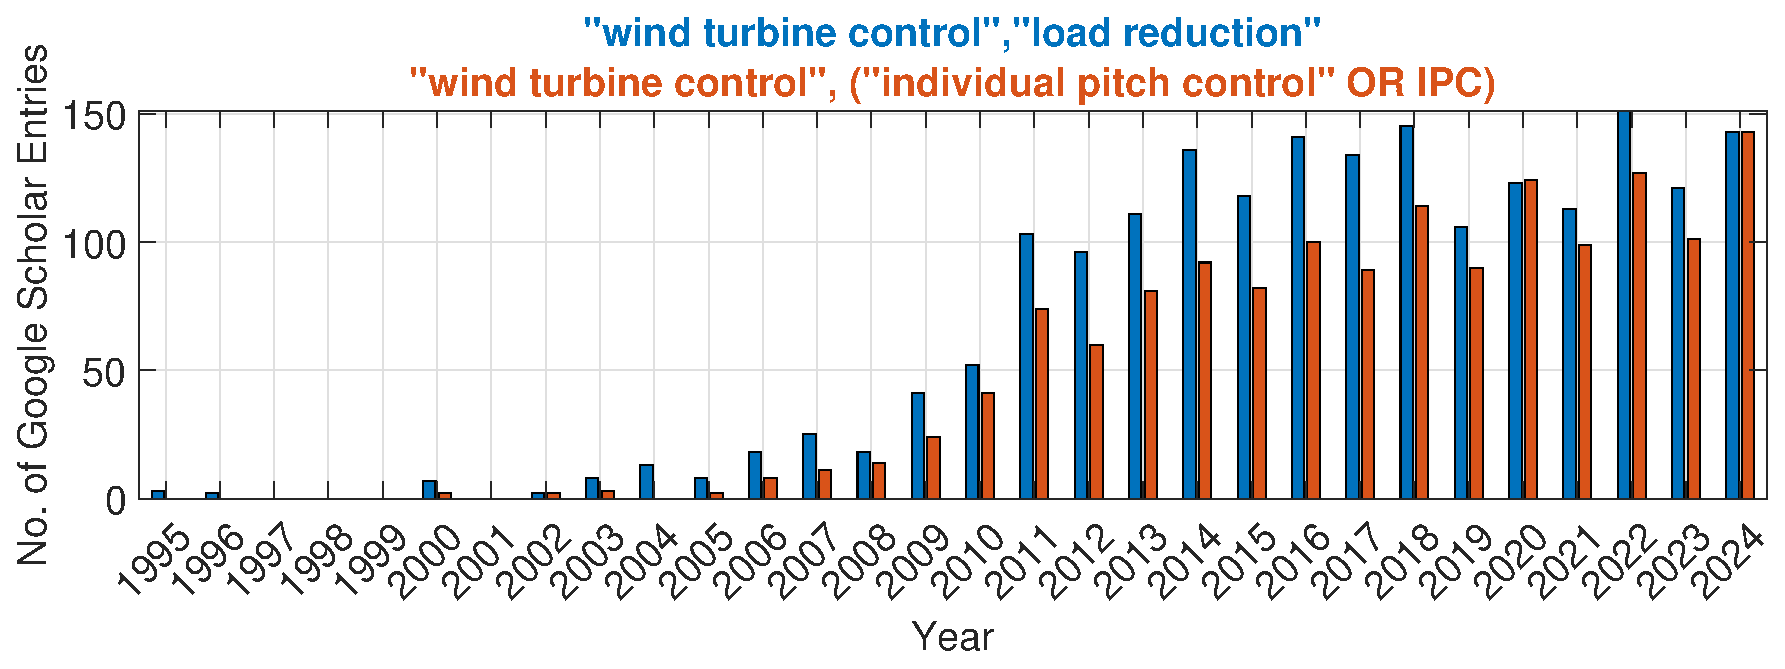
\includegraphics[width=0.85\textwidth]{figures/Figures_ADi/googleWordleWTLoadRedIPC.eps}} \\ %\hfill 
 \subfloat[Search term ``model predictive control"]{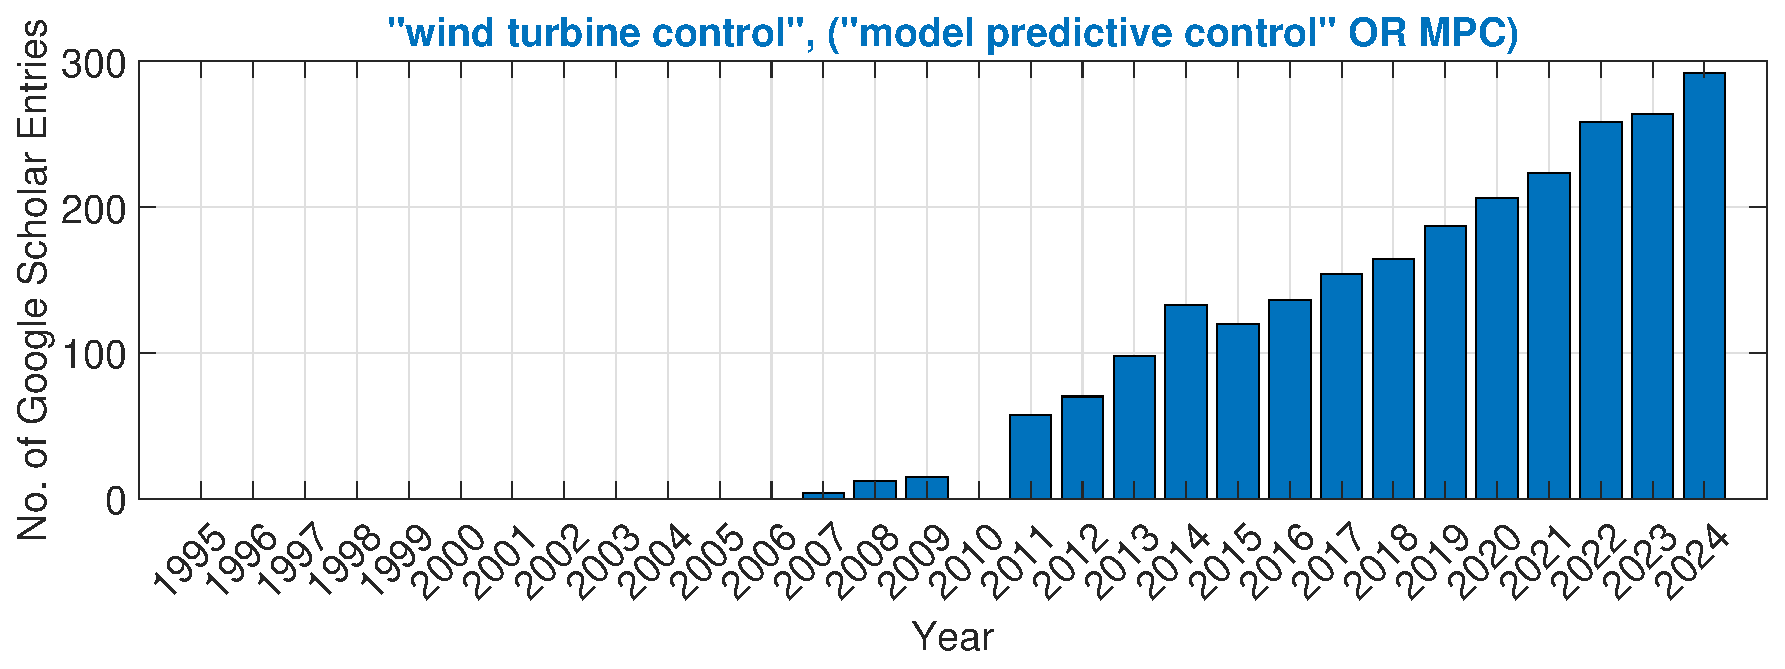
\includegraphics[width=0.85\textwidth]{figures/Figures_ADi/googleWordleWTMPC.eps}} %\hfill
\caption{Number of Google Scholar results by year for the search term ``wind turbine control" and different additional search terms}
\label{fig01:WTstatistics}
\end{figure}

\begin{figure} [h]
 \center
\subfloat[Search terms ``axial induction control" and ``wake redirection control"]{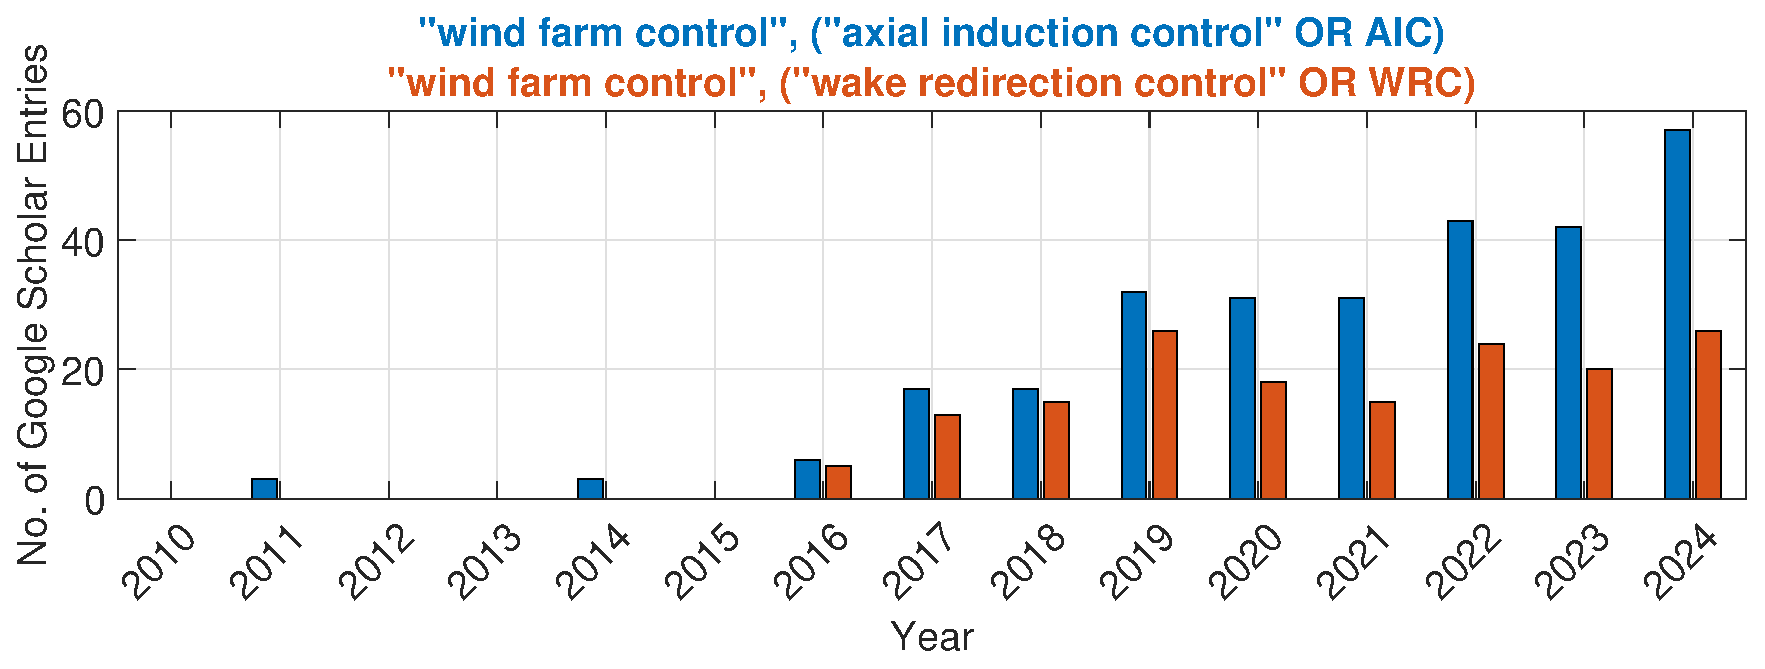
\includegraphics[width=0.85\textwidth]{figures/Figures_ADi/googleWordleWFAICWRC.eps}}\\
\subfloat[Search term ``Koopman"]{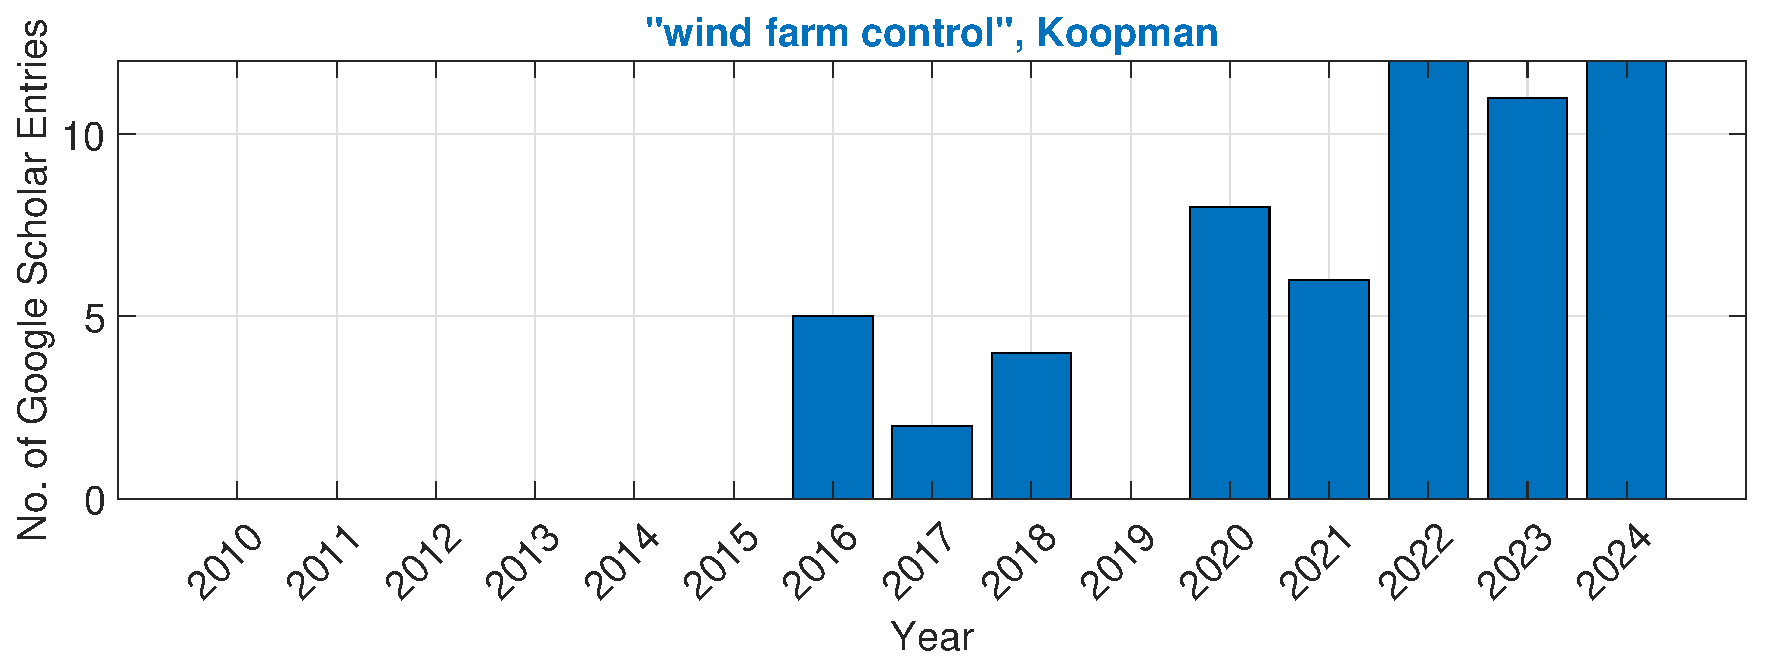
\includegraphics[width=0.85\textwidth]{figures/Figures_ADi/googleWordleWFKoopman.eps}}\hfill
\caption{Number of Google Scholar results by year for the search term ``wind farm control" and different additional search terms }
\label{fig01:WFstatistics}
\end{figure}

Figure~\ref{fig01:WTstatistics}(a) shows a significant increase of number of published studies over the past approximately fifteen years and a continuously high number, exceeding 100 publications each year, after 2021 for both search terms ``load reduction" and ``individual pitch control". Figure~\ref{fig01:WTstatistics}(b) shows a nearly exponential increase in publication number for MPC and wind turbine control, with more than 200 publications found on Google Scholar each year after 2020.  
%
But while there is extensive literature on load reduction of wind turbines, both via IPC, and MPC, relatively few works explicitly examined using quasi-Linear Parameter Varying (qLPV) MPC, so called qLMPC schemes. In \cite{Bianchi2007}, modeling wind turbines as qLPV is described, but not within an MPC, but within an $H_{\infty}$ control approach. In \cite{kumar2010FeedbackLinLQR} a non-linear turbine model is derived and a feedback linearization controller is compared to a Linear Quadratic Regulator (LQR), showing better performance around rated wind speed. The first work to suggest explicitly using the qLMPC introduced in \cite{cisneros2016efficient} for wind turbine control is \cite{mulders2020preventing}, where it is used to derive optimal torque control for tower load reduction as a Single-Input Single-Output (SISO) scheme. This work was followed by a study leveraging a Kalman filter to estimate unmeasurable periodic side-to-side loads in wind turbines, addressing fatigue challenges in tall, slender towers \cite{pamososuryo2022loadestimation}. In \cite{pamososuryo2022individual,pamososuryo2023convex} a convex economic MPC is developed for IPC to actively damp side-to-side tower motion. In \cite{feng2022economic} an economic MPC is used to reduce the load distributed over the turbine tower. Recently, the application of velocity-based qLMPC, an algorithm published in \cite{cisneros2020velocity} for reduction of side-to-side tower motion was investigated in \cite{fonseca2024windTurbineSideSide}. In parallel, IPC has been applied in various studies to enable blade root moment reduction: Promising simulation results exist with different control algorithms, e.g., Proportional-Integral-Derivative (PID) \cite{hoffmann2018load}, Linear Quadratic Gaussian (LQG) \cite{selvam2009feedback}, and MPC schemes \cite{petrovic2021mpc}. Field tests confirm the potential of IPC, see \cite{ossmann2021field} and \cite{bossanyi2012advanced}. Recently, TEFs for wind turbines have been suggested for blade root load reductions in \cite{zhang2015parameter} and \cite{bergami2017highfidelity}. As TEF add an additional degree of freedom to the wind turbines' actuation, there are also studies combining the two methods: In \cite{wilson2009combined}, the standard deviation of blade root flapwise bending moments is reduced up to 32\% for two wind test cases with turbulence class A, at 16\,m/s and 20\,m/s mean wind speed. Turbulence class A at 18\,m/s mean wind speed is used in \cite{henriksen2013model} to investigate the trade-off between load reduction and actuator activity. In \cite{he2018combined}, the blade root flapwise moments and blade tip out-of-plane deflection are both reduced by over 50\%, while also decreasing tower moments for a wind test case of turbulence class B at 20\,m/s. In Chapter~\ref{sec:WindTurbineqLPVModels} of this thesis the design of two qLPV models, one modelling the tower and rotor dynamics as proposed in the previously cited studies and one additionally including blade and generator dynamics as suggested in \cite{Bianchi2007} is presented. In Chapter~\ref{sec:Application to Wind Turbine Control4} the implementation of a velocity-based qLMPC controller is discussed, with a focus on power reference tracking and fore-aft tower motion reduction. This is followed by the design and evaluation of an IPC controller and a combined IPC–TEFC control strategy, which are directly compared to the qLMPC scheme across multiple performance criteria.

Similarly to wind turbine control, Figure~\ref{fig01:WFstatistics}\,(a) shows that for the last ten years wind farm control is a widely studied subject, but that the number of studies leveraging Koopman theory is more limited, see Figure~\ref{fig01:WFstatistics}\,(b). The survey paper \cite{houck2022review} categorizes wake management into AIC, WRC, a combination of WRC-AIC, and active wake control. Currently, WRC, which uses yaw to redirect wakes, is the most frequently investigated technique and likely to achieve broader industrial application. However, applying WRC to real wind turbines will require combining it with thrust control via power control for below-rated wind speeds and pitch control for above-rated wind speeds.

Of the 8 papers mentioned in \cite{houck2022review} to use combined WRC-AIC, \cite{jimenez2010application} investigates the wake centerline deflection and spread in simulations and \cite{castillo2020wind} in wind tunnel tests. In \cite{bossanyi2018combining} an increase in production and decreased loads, both in the lower one-digit percentage range, is demonstrated in simulations. A lower two-digit percentage increase in power is reported in \cite{cossu2020wake}, based similarly on simulations. In \cite{fleming2016computational} it is concluded that combined WRC-AIC is the control technique resulting in the lowest grid reference tracking error. In the three papers, \cite{park2013wind}, \cite{park2015cooperative}, and \cite{en10070852}, the authors use different, purely data-driven techniques to optimize a combination of induction and yaw control. The advantage of combined WRC-AIC is summarized in \cite{houck2022review} by noting that lowering the thrust of the upstream, misaligned turbine may provide the optimal balance of power increase and load reduction, if wake steering is insufficient to steer a wake completely away from a downstream turbine. But it is mentioned that combined WRC-AIC still requires prior optimizations or real-time computing to implement in the field. However, with a data-driven technique like Koopman MPC a real-time controller can be implemented for wind farms. 

The idea of using the Koopman matrix, a linear approximation of the Koopman operator, to model wind flow and wakes in a wind farm was first suggested in \cite{annoni2016wind} and extended to farm control via axial induction control in \cite{annoni2016sparsity}. The potential of Dynamic Mode Decomposition (DMD) for wake models was also pointed out in \cite{proctor2016including} which provides a comparison between DMD and the proper orthogonal decomposition for fluid dynamics modelling. In \cite{munters2017optimal} a MPC is set up with the wind farm dynamics modelled as Large Eddy Simulation (LES) and hence based on Navier-Stokes Equation (NSE) and in \cite{munters2018data} the idea of using Koopman to model LES is discussed. In \cite{debnath2017towards} the structure of a wake, simulated via LES, is analyzed. Based on their previous work, it is discussed \cite{annoni2018sparse} how lidar sensors are to be placed in wind farms to extract a maximum amount of information. In \cite{ali2020data} the varying flow velocities over the blade span are modelled with a linear model derived via an Extended DMD (EDMD), taking the forces acting on the rotor excited by the control inputs into account. \cite{chen2020data} discusses using DMD to model the wake flow dynamics. A proof-of-concept for Koopman matrices derived via  Extended Input-Output DMD (EIODMD), with the resulting linear state-space models used as basis for MPC, is given in \cite{Cassamo.2020}, which investigates AIC, and in \cite{cassamo2021model} for WRC. In Chapter~\ref{sec:ApplicationtoWindFarmControl} of this thesis the application of Koopman MPC to AIC as well as a combination of AIC and WRC is discussed. 

\section{Main Contributions}
This section outlines the primary contributions of this thesis in the field of wind turbine and wind farm control. The research focuses on the integration of novel physics-based and data-driven MPC techniques to optimize wind turbine and wind farm performance. In all contributions, care was taken to make the algorithms real-time capable, with convergence rates considerably below the 10\,ms sampling rate of wind turbine controller, and to only use input signals that can realistically be expected to be available during the operation of a real wind turbine. Although the applicability of these algorithms remains at the proof-of-concept stage, they could be applied to wind turbine control with relatively little modification, assuming the necessary sensors and actuators are available. 

The first contribution of this thesis is the development of a real-time capable, velocity-based qLMPC for wind turbine control across the entire operating range. Leveraging Lagrange's equations, a first-principles model incorporating the physics, mechanics, and aerodynamics of the wind turbine was formulated. This model was then utilized in an MPC framework, reformulated as a Quadratic Programming (QP) problem to achieve real-time convergence within millisecond timescales. This work was published in \cite{dittmer2021velocity}.
%
Furthermore, the development and rigorous verification of an active aerodynamic load control system integrating IPC with TEF control is presented. While previous studies had suggested the potential of combining IPC and TEF for wind turbine control, our study, published in \cite{dittmer2024combined}, was the first to rigorously demonstrate the effectiveness of this approach across a wide range of wind speeds. The research evaluated the FAST turbine model extended  with TEFs, using a training dataset and two independent verification datasets, to ensure a comprehensive performance assessment. The results confirmed a significant reduction in blade root out-of-plane moments and tower base loads.

The second contribution is the development of an adaptive Koopman MPC framework for wind farm control, marking the first time this efficient update mechanism has been applied in wind farm control simulation. Inspired by the Navier-Stokes equations governing turbine interaction, this approach leverages Koopman lifting functions to construct a Koopman matrix for predicting wake interactions and effective wind speed. Computational efficiency is achieved by updating the Koopman matrix only when discrepancies between past predicted and actual wind data are detected. This work builds upon prior research on qLMPC for wind farm control, enhancing its applicability by highlighting its potential to adapt to sudden changes in operation. The findings were published in \cite{dittmer2022data}, extending our earlier work on non-adaptive MPC \cite{sharan2022Koopman}.

Additionally, a data-driven Koopman MPC approach for combined thrust and yaw control in wind farms is demonstrated. Combining thrust and yaw control was motivated by the fact that, due to the slowness of yaw movements, practical implementations of WRC must be combined with pitch and torque control for dynamic load management and efficient power regulation. This combination is driven by the superior power yields achievable with WRC compared to AIC. By incorporating WRC-AIC into the previous AIC framework, this approach achieved a roughly 10\% increase in power output under steady-state conditions and enabled the system to follow grid power references with higher power demands. This data-driven approach directly estimates farm power using a linear system based on the Koopman matrix, eliminating the need for detailed wake modeling. The Koopman MPC framework, presented in \cite{dittmer2023koopman}, demonstrates promising results in achieving reference tracking at reduced actuator activity.

The effectiveness of the proposed MPC controllers is validated through comparative analyses against non-predictive schemes and baseline MPC approaches. Results indicate improvements in power tracking, load reduction, and control quality. Additionally, the wind farm Koopman MPC demonstrates performance with reduced measurement requirements, offering practical advantages over solutions presented in previous studies.

\section{Thesis Structure}
This thesis is organized as follows: Chapter \ref{sec:Background} provides a comprehensive review of the physics of wind, wind turbine and wind farm dynamics, and their control. The fundamental ideas of qLPV models and MPC are presented. The chapter also introduces the Koopman operator and DMD.

Chapter~\ref{sec:WindTurbineqLPVModels} focuses on the development of a qLPV wind turbine model. Two models are derived: one modeling the rotor speed and tower movements only, and one, using Lagrange's equations, modeling additionally blade movements and generator speed. The quality of the two qLPV models is verified across the entire turbine operating range in both frequency and time domains using the software FAST.

Chapter~\ref{sec:Application to Wind Turbine Control4} presents the work on wind turbine control, encompassing both the velocity-based qLMPC framework and the active aerodynamic load control system integrating IPC with TEF control. The qLMPC framework is discussed in terms of its reformulation as a  QP problem for real-time implementation. Its performance is evaluated for power tracking and load reduction, with comparative analyses against baseline control methods. The chapter also discusses the effectiveness for reducing blade root and tower loads over a wide range of wind speeds with the IPC-TEF approach.   

Chapter~\ref{sec:ApplicationtoWindFarmControl} describes Koopman MPC for wind farm control: an adaptive Koopman MPC using thrust control and a Koopman MPC for combined thrust and yaw control. The software WFSim and enhancements necessary to evaluate the presented algorithms are discussed. The adaptive Koopman MPC leverages efficient update mechanisms to deal with abrupt changes, while the combined thrust and yaw approach integrates WRC with AIC to increase power yield. The chapter evaluates the proposed methods for power output improvement, grid reference tracking, and actuator activity reduction.

Chapter~\ref{Conclusions} summarizes the main contributions and findings of the thesis 
and discusses the practical implications of the proposed control strategies. It provides 
a discussion of existing challenges, concretely relating to sensor 
integration, actuator degradation, and validation in higher-fidelity simulation 
environments. Finally, it outlines directions for future research, including the 
extension to more realistic wind conditions and the use of Neural Network~(NN) based 
lifting functions as an alternative to physically motivated observables.



    \chapter{Background} \label{sec:Background}

Simulations can only evaluate the effects of different control algorithms meaningfully if the underlying simulation models reasonably resemble reality. This background chapter provides an overview of the physical models used to describe the behavior of wind in Section~\ref{sec:Wind} and wind turbines in Section~\ref{sec:WindTurbines}. The interaction of wind turbines in farms via wake effects is described in Section~\ref{sec:WakeModels}. Baseline control schemes for both wind turbines and wind farms, against which the designs in this thesis are evaluated, are also presented in these sections. Section~\ref{sec:Control-Theoretic Background} presents the mathematical foundations of the two modeling frameworks used in this thesis, i.e., qLPV for wind turbines and Koopman for wind farms, followed by the MPC framework applied to both.

\section{Wind} \label{sec:Wind}

While wind, unlike conventional energy sources, cannot be controlled, its dynamics are well studied and understood. Detailed information on the aerodynamics of wind and wind turbines can be found, for example, in~\cite{hansen2015aerodynamics} and~\cite{hau20084}. The following section provides an overview of the related chapter in~\cite{Bianchi2007}, which summarizes the physics of wind.

Standardized wind models from the International Electrotechnical Commission (IEC) are used for testing and for the certification of controllers. The economic viability of a wind energy project, and hence decisions that need to be made prior to construction, such as number and exact location of turbines in a farm or turbine type, depend on the temporal and spatial wind distribution at the investigated site. These wind measurements also influence the choice of IEC wind models used for controller synthesis and closed-loop controller testing.

Wind is generated by temperature differences caused by uneven solar heating of the atmosphere. Wind can be classified into large-scale airflows, called geostrophic wind, which occurs in all layers of the atmosphere, and local wind. Local wind flows develop in the lower layer of the atmosphere, which extends up to a height of 100\,m and is therefore affected by geographical features and surface topography.

The kinetic energy frequency distribution of wind speeds follows a typical pattern, called the van der Hoven spectrum. The spectrum has two peaks, one at approximately 0.01 cycles per hour, representing a four-day cycle, and another at around 50 cycles per hour, roughly corresponding to one-minute cycles. These peaks are separated by an energy gap, indicating lesser energy content in wind speeds with frequencies between ten minutes and two hours. The low-frequency side of the spectrum is associated with geostrophic wind, while the high-frequency side represents local wind speeds, including turbulence. The aeroelastic forces that turbines are subjected to over their lifespan include mean wind speeds, i.e., constant stationary air movement, and stochastic turbulence. Hence, ten-minute time series with different mean values and different turbulence classes are traditionally used for controller testing and load analysis in wind energy applications.

The quasi-steady mean wind speed $\bar{V}$ at a site is the most important factor influencing the potential profitability of a wind energy project and the selection of appropriate wind turbines to maximize the annual energy production over the turbines' lifespan. The probability distribution of mean wind speeds is often predicted based on long-term measurements and can typically be approximated by the Weibull distribution:
\begin{equation}
    f_{\text{WB}}(\bar{V}) = \frac{k_{\text{WB}}}{C_{\text{WB}}}\left(\frac{\bar{V}}{C_{\text{WB}}}\right)^{k_{\text{WB}}-1}e^{- (\bar{V}/C_{\text{WB}})^{k_{\text{WB}}}}
\end{equation}
with shape and scale coefficients, $k_{\text{WB}}$ and $C_{\text{WB}}$, respectively, describing the probability of different wind speeds occurring at the site.

Mean wind speed also varies with height above ground level as surface roughness and obstacles affect wind speed through frictional forces. This spatial speed variation is called wind shear and can be described by different models, among them the exponential law:
\begin{equation}
    \bar{V}(z) =  \bar{V}(z_{\text{ref}})\left(\frac{z} {z_{\text{ref}} }\right)^{\alpha_{\text{shear}}} 
\end{equation}
where $z$ is the height above ground, $z_{\text{ref}}$ is a reference height, often 10\,m, and $\alpha_{\text{shear}}$ is the wind shear exponent. In \cite{Bianchi2007}, values for sand, mown and high grass, and suburban areas are given, varying from 0.10 to 0.32. In this work, the commonly used surface roughness exponent $\alpha_{\text{shear}} = 0.2$ is used.

While turbulence has a minor influence on Annual Energy Capture (AEC), it significantly impacts aerodynamic loads and power variance. Power variance is often called power quality, as maintaining a smooth power output is important, especially in smaller networks.

Turbulence is stochastically described by its power spectrum. Two widely used models are the von K\'arm\'an and Kaimal spectra:
\begin{equation}
    \Phi_{\text{K\'arm\'an}}(\omega) = \frac{K_V}{(1 +(\omega T_V)^2)^{5/6}} \quad \text{and} \quad \Phi_{\text{Kaimal}}(\omega) = \frac{K_V}{(1 +\omega T_V)^{5/3}}
\end{equation} 
where $\omega$ is the angular frequency, $T_V$ is the frequency bandwidth of the turbulence, and $K_V$ describes the turbulence power. For the von K\'arm\'an spectrum, they are approximated as:
\begin{equation}
    K_V = 0.475 I_v^2 \frac{L_v}{\bar{V}(z)} \quad \text{and} \quad T_V = \frac{L_v}{\bar{V}(z)}
\end{equation}
with the turbulence intensity $I_v$, which represents the ratio of the standard deviation of wind speed fluctuations to the mean wind speed, and the correlation length $L_v$, which indicates the scale of turbulence in space. The von K\'arm\'an model is implemented in the FASTTool, and therefore all the turbulent wind model test cases presented in this thesis leverage it.

The turbulence intensity, which depends on the height of the turbine and the terrain of a potential site, is an important factor in site selection. Higher turbulence intensity leads to increased aerodynamic loads on turbine structures, influencing the durability and performance of wind turbines.

\section{Wind Turbines} \label{sec:WindTurbines}

Wind turbines extract kinetic energy from the wind and convert it into other energy forms, most often electricity. In this section, commonly used mathematical representations based on the physics governing wind turbine behavior are provided, and a state-of-the-art control scheme for modern wind turbines is discussed.

\subsection{Wind Turbine Simulation Models}\label{windTurbineModel}
Depending on the application, different models are used to describe the physical effects of a wind turbine. In their simplest form, wind turbines can be modeled as an energy sink using the actuator disk model, which is the model used in WFSim~\cite{boersma2018control}. Alternatively, the Blade Element Momentum (BEM) model can be used directly, as in FAST~\cite{jonkman2005fast}, or via lookup tables for rotor thrust and torque to include the effect of varying rotor speed and pitch angles on the forces and moments. All models in this thesis are parameterized for the NREL 5MW reference 
turbine, with its physical parameters listed in Table~\ref{table:1}.

\subsubsection{Actuator Disk Model}
The amount of energy extracted from the wind depends on the wind speed difference between the wind in front of the turbine and the wind behind it. Figure~\ref{fig:ActDiscModel} visualizes the airflow through a rotor disk, showing the wind speeds, pressures, and corresponding areas of the airflow far ahead and far behind the turbine, as well as at the rotor.
%
\begin{figure}[ht]
    \center
    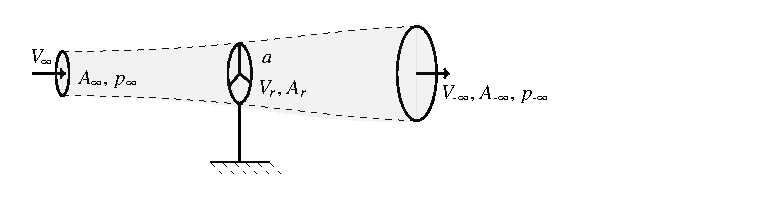
\includegraphics[width=0.76\textwidth,trim={0cm 0.3cm 3.5cm 0.4cm},clip]{figures/figuresBlockDiagram_IFAC23/testTurbineBetz.pdf}
    \caption{Airflow through a wind turbine, modelled as an actuator disk, adapted from \cite{Bianchi2007}.}
    \label{fig:ActDiscModel}
\end{figure}
%
The available amount of wind power $P_w$ and the amount of power $P_r$ extracted by the turbine rotor at the rotor area $A_r$ are given by:
\begin{eqnarray} \label{eq:PwPt}
    P_w = \frac{1}{2} \rho_a A_r V_{\infty}^3,\quad\text{and} \quad  P_r = c_P P_w,
\end{eqnarray}
where $\rho_a$ is the air density, $V_{\infty}$ is the freestream wind speed, and $c_P$ is the power coefficient. The ratio of freestream wind speed $V_{\infty}$ to the mean wind speed at the turbine rotor disk $V_r$, also called the effective wind speed, is:
\begin{eqnarray} \label{eq:ainduct}
    V_r = (1-a)V_{\infty},
\end{eqnarray}
where $a$ is the axial induction factor. The thrust $F_{T,r}$ acting on the turbine can be calculated from the pressure difference $\Delta p_r$ at the rotor disk. This pressure difference depends on the freestream wind and the recovered wind speed $V_{\text{-}\infty}$ far behind the turbines, leveraging Bernoulli's equation:
\begin{equation}\label{eq:pVBernoulli}
    \Delta p_r = \frac{1}{2} \rho_a(V_{\infty}^2  - V_{\text{-}\infty}^2 ).
\end{equation}
The thrust $F_{T,r}$ can be determined either from its rotor area and the pressure difference in Equation \eqref{eq:pVBernoulli}:
\begin{eqnarray} \label{eq:Ft1}
    F_{T,r} = A_r \Delta p_r =  \frac{1}{2} \rho_a A_r (V_{\infty}^2  - V_{\text{-}\infty}^2 ) 
\end{eqnarray}
or alternatively as the product of the air mass flow through the rotor area $\dot{m}_a$ and the wind speed difference:
\begin{eqnarray} \label{eq:Ft}
    F_{T,r} =  \dot{m}_a  (V_{\infty} - V_{-\infty}) = \rho_a A_r V_r (V_{\infty} - V_{\text{-}\infty}).  
\end{eqnarray}
From Equations \eqref{eq:ainduct}, \eqref{eq:Ft1}, and \eqref{eq:Ft}, the thrust of the rotor can be calculated as:
\begin{align} \label{eq:Ftall}
    F_{T,r} = 2a(1-a) \rho_a A_r V_{\infty}^2.
\end{align}
Combining Equations \eqref{eq:PwPt} to \eqref{eq:Ft} and using the fact that $P_r = F_{T,r} V_r$, the relationship between the axial induction factor $a$ and the power coefficient $c_P$ is:
\begin{equation}\label{eq:cpFromA}
    c_P(a) = 4a(1-a)^2,
\end{equation}
with the axial induction factor maximizing power yield given by $a^* = 1/3$ and the maximum $c_P(a^*) = 16/27$, known as the Betz limit. The wind speed difference and, consequently, the amount of power extracted from the wind, is influenced in real turbines by changing the generator speed and adjusting the blade pitch angle, both of which affect the turbine's rotor speed.

\subsubsection{Blade Element Momentum Theory}
The actuator disk model is a significantly simplified representation of the physics of a wind energy conversion system (WECS). Wind turbines consist of an aerodynamic subsystem, a flexible drivetrain, and a power generator, with the aerodynamic subsystem responsible for converting the available kinetic energy of the wind into useful mechanical energy through the rotor blades \cite{SaMuAlBe18}. 

Figure~\ref{figBEMModel} visualizes the local flow conditions and force components at a blade element, as used in Blade Element Momentum Theory (BEMT). In this model, the rotor is divided into small segments, each treated as an independent airfoil.
\begin{figure}[ht] %  %The Blade Element Momentum (BEM) model, as visualized in Figure \ref{figBEMModel}, refines the actuator disk model by incorporating the detailed aerodynamic behavior of individual rotor blades. 
    \center
    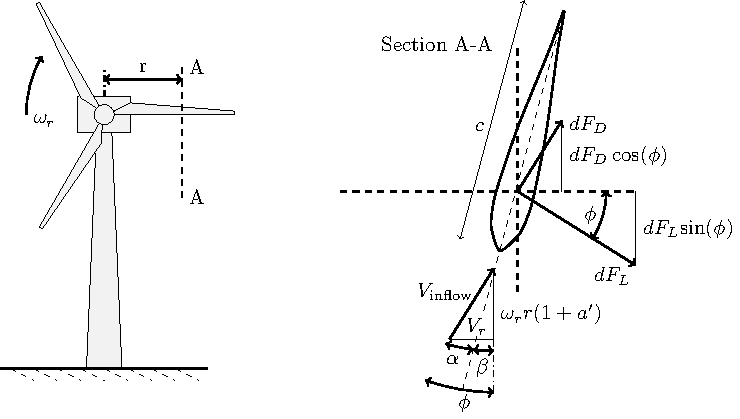
\includegraphics[width=0.96\textwidth,trim={0cm 0cm 0cm 0cm},clip]{figures/figuresBlockDiagram_IFAC23/turbineAirfoilBem.pdf}
    \caption{Local airflow and forces on a blade element of width $dr$ at radial position $r$, based on \cite{hansen2015aerodynamics} and adapted from \cite{weiss2016regelungstechnische}.} 
    \label{figBEMModel}
\end{figure}

BEMT combines the principles of blade element theory, which calculates the forces on each blade segment based on local airflow conditions, and momentum theory, which models the changes in wind velocity and pressure as air passes through the rotor disk. The lift and drag forces $dF_L$ and $dF_D$ on each blade element located at a radial position $r$ are determined by the angle of attack $\alpha$, the pitch angle $\beta$, the local airspeed $V_\text{inflow}$, the rotational speed of the rotor $\omega_r$, and the tangential flow induction factor $a^{\prime}$. The wind speed component $V_r$ is calculated from the freestream wind speed $V_{\infty}$ and the axial induction factor $a$ as described in Equation~\eqref{eq:ainduct}. The forces $dF_L$ and $dF_D$ are used to determine the thrust $F_{T,r}$ and torque $T_r$ generated by the rotor. 

The lift and drag forces, which act perpendicular and parallel to the inflow of a blade section with chord $c$ and width $dr$, are:
\begin{align} \label{eq:dFldFd}
    dF_L &= \frac{1}{2} \rho_a V^2_{\text{inflow}} c_L(\alpha)cdr,\\
    dF_D &= \frac{1}{2} \rho_a V^2_{\text{inflow}} c_D(\alpha)cdr,
\end{align}
where the lift and drag coefficients $c_L$ and $c_D$ depend on the angle of attack $\alpha$. As shown in Figure \ref{figBEMModel}, the angle $\phi$ between the local flow direction and the rotor plane is the sum of the angle of attack $\alpha$ and the pitch angle $\beta$. The thrust and torque of each segment can be calculated as:
\begin{align} \label{eq:dFTrdTr}
    dF_{T,r} &= dF_{L}\cos\phi + dF_D \sin\phi,\\
    dT_r &= (dF_{L} \sin \phi - dF_D \cos\phi) r.
\end{align}
The relative wind speed at the blade depends on its perpendicular and tangential components:
\begin{align} \label{eq:dFTrdTr1}
    V_{\text{inflow}} = V_{\infty}\sqrt{(1-a)^2 + \left(\frac{\omega_{r}r}{ V_{\infty}}(1+a^{\prime})\right)^2}\text{ and } \tan \phi = \frac{V_{\infty}}{\omega_r r} \frac{1-a}{1+a^{\prime}}.
\end{align} % where $a$ is the axial induction factor and $a^{\prime}$ is the tangential induction factor. 
The two induction factors $a$ and $a^{\prime}$ can be calculated if the blade element properties $c_L(\alpha)$, $c_D(\alpha)$, $r$, and $dr$ are known, as well as the current values of variables influencing the local force. These variables include $\rho_a$, $V_{\infty}$, $\omega_r$, and $\beta$. The BEM theory, as implemented in FAST, assumes steady, incompressible flow and calculates the rotor's performance iteratively using Equations \eqref{eq:pVBernoulli} to \eqref{eq:dFTrdTr1}. Thus, the interaction between the blade elements and the wind is considered in computing the forces, moments, and movements of the WECS. This iterative process is used to simulate performance under different wind conditions. The movement of the blades and tower is calculated in FAST using a linear modal representation, which leverages that the deflection angles are relatively small.

The wind turbine modeling approaches discussed in this section account for the influence of wind-speed variations on turbine operation. However, the instantaneous power extracted from the wind depends not only on the available wind speed but also on the turbine’s control inputs, generator speed, and blade pitch angle. The next subsection provides an overview of state-of-the-art wind turbine control strategies.


\subsection{Wind Turbine Control} \label{sec:WindTurbineControl}

All modern wind turbines use a control system to regulate rotor speed. The control settings of a wind turbine are determined by the energy available in the wind as well as economic considerations. Figure \ref{fig:WindREgion} visualizes the power output at different wind speeds.

\begin{figure}[ht]
\center
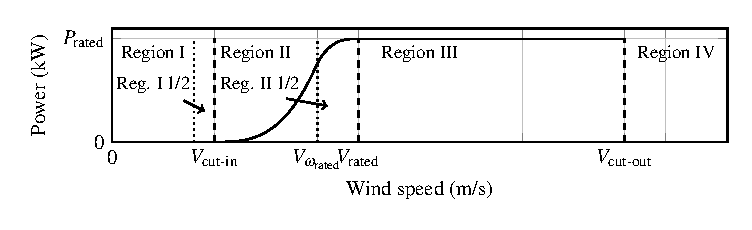
\includegraphics[width=0.8\textwidth,trim={0.5cm 0.4cm 0.0cm 0.3cm},clip]{figures/Figures_ADi/windRegionen.pdf}
\caption{Power output curve in Regions I to IV, based on the control region definitions for the NREL 5-MW reference turbine in \cite{jonkman2009definition}.}\label{fig:WindREgion}
\end{figure}

At very low wind speeds, below the so-called cut-in wind speed $V_{\text{cut-in}}$, the power that could be produced would not cover the operating costs. The wind speed region up to the cut-in wind speed is referred to as Region I. The wind speed region between the cut-in wind speed and the rated wind speed $V_{\text{rated}}$ of a turbine, i.e., the wind speed corresponding to the rated power of the turbine, is called Region~II. 

For wind speeds above the rated wind speed, the blades are pitched to keep the power output constant and to reduce excessive mechanical loads that would otherwise shorten the turbine's operational lifespan. At very high wind speeds, above the cut-out wind speed $V_{\text{cut-out}}$, the turbine stops operating. Region III is the wind speed range between rated and cut-out wind speed, while Region IV refers to wind speeds above the cut-out wind speed.

At each wind speed between the cut-in and cut-out wind speeds, a control system ensures the most profitable power output by regulating the generator torque $T_g$ and the blade pitch angle $\beta$. Generator torque is used to maximize power yield at wind speeds in Region~II. The blade pitch is used to maintain a constant power output at rated power for wind speeds above the rated wind speed and below the cut-out wind speed in Region~III. The power controller receives feedback from the generator rotational speed $\omega_g$ across all operating regions. 

In this work, the power controller available within TU Delft's FASTTool \cite{mulders2020wind} is used as a baseline, see Table~\ref{table:pitch_ctrl} for its parameters. FASTTool features a MATLAB graphical user interface for setting up simulations and tuning control parameters for an underlying Simulink model, which represents the dynamics of the NREL 5MW turbine. The underlying physical principles are detailed in \cite{jonkman2009definition}. 


\subsubsection{Generator Torque Control}

In Regions I\,1/2 and II, the generator torque is governed by the so-called $k\omega^2$ control law, which is implemented as a tabulated function of the generator speed $\omega_g$. In Region~I\,1/2, the start-up phase just below the cut-in wind speed, see Figure~\ref{fig:WindREgion}, a multiplication factor is applied to compute the reference generator torque $T_{g,\text{ref}}$. In most of Region~II, an optimal factor $K^*$ is multiplied by the square of the rotational speed.

The upper portion of Region II, just below the rated wind speed, is referred to as Region~II\,1/2. In this transition zone, a smooth linear interpolation is applied up to the rated rotational speed. This ensures a seamless transition within Region~II while also maintaining compliance with noise emission regulations and limiting excessive mechanical loads. These controller settings, originally defined in \cite{jonkman2009definition}, have been implemented without modifications in \cite{mulders2020wind}, preserving both the algorithmic structure and parameter values.

\subsubsection{Blade Pitch Control} 

In Region III, the collective pitch control strategy relies on a scheduled proportional-integral (PI) controller, where the proportional and integral gains, $K_P(\omega_g)$ and $K_I(\omega_g)$, are dynamically adjusted based on the generator speed. This adaptive gain scheduling enhances the tracking of the maximum allowable rotor speed. The gain values used in this implementation remain unchanged from those provided in the original FASTTool repository.

The derivation of these gains follows from \cite{jonkman2009definition}. The difference between the aerodynamic torque $T_r$ and the generator torque $T_g$, with the latter multiplied by the gear ratio $N_g$, is equal to the product of drivetrain inertia $J_{s}$ and the rotor acceleration $\Delta \dot{\omega}_r$:

\begin{equation} \label{eq:Tr1_background}
T_r -N_g T_g = (J_r + N_g^2 J_g) \frac{d}{dt}(\omega_{\text{rated}} + \Delta \omega_r) = J_{s} \Delta \dot{\omega}_r,
\end{equation}
where $J_r$ and $J_g$ are the rotor and generator inertias, respectively. The aerodynamic and generator torques, derived from the rated power $P_{\text{rated}}$, can be approximated as Taylor series expansions:

\begin{eqnarray}
T_g(\omega_r) &=& \frac{P_{\text{rated}}}{N_g \omega_r} \approx  \frac{P_{\text{rated}}}{N_g \omega_{\text{rated}}} - \frac{P_{\text{rated}}}{N_g\omega_{\text{rated}}^2} \Delta \omega_r,  \label{eq:Tg}\\
T_r(\beta) &=& \frac{P(\beta,\omega_r)}{\omega_r}   \approx \frac{P_{\text{rated}}}{\omega_{\text{rated}}} + \frac{1}{\omega_{\text{rated}}}\Big(\frac{\partial P}{\partial \beta}\Big) \Delta \beta.  \label{eq:Tr_background}
\end{eqnarray}
%
The desired change in pitch angle, $\Delta \beta$, is calculated based on the rotor speed deviation $\Delta \omega_r$ using a proportional-integral-derivative (PID) controller:

\begin{eqnarray} \label{eq:PID}
\Delta \beta = K_P N_g \Delta \omega_r + K_I \int_{0}^{t}N_g \Delta \omega_r dt + K_D N_g \Delta \dot{\omega}_r.
\end{eqnarray}
%
Substituting Equation~\eqref{eq:PID} into Equation~\eqref{eq:Tr_background} and incorporating the relationships from Equations \eqref{eq:Tr1_background} and \eqref{eq:Tg} leads to the final control formulation with the substitute state $\dot{x} = \Delta \omega_r$ and derivative $\mathcal{P}_\beta = \left( -\frac{\partial P}{\partial \beta} \right)$:

\begin{equation}\label{eq:PID2} 
\underbrace{\left[ J_{s} + \frac{\mathcal{P}_\beta}{\omega_{\text{rated}}} N_{g} K_D \right]}_{M_{x}} \ddot{x}(t) 
+ \underbrace{\left[ \frac{\mathcal{P}_\beta}{\omega_{\text{rated}}} N_{g} K_P - \frac{P_{\text{rated}}}{\omega_{\text{rated}}^2} \right]}_{C_{x}} \dot{x} (t)
+ \underbrace{\left[ \frac{\mathcal{P}_\beta}{\omega_{\text{rated}}} N_{g} K_I \right]}_{K_{x}} x(t) = 0.
\end{equation}
%
The PID gains are determined to achieve the desired natural frequency and damping ratio, which, in turn, dictate how the mass $M_{x}$, damping $C_{x}$, and spring term $K_{x}$ should be set through the control parameters. The value of  $\mathcal{P}_\beta$, i.e., the sensitivity of the aerodynamic power to the blade pitch, can be calculated for the different operating points and is provided in \cite{jonkman2009definition}. 

In the implementation of \cite{mulders2020wind}, a gain-scheduled PI controller is used by default, with the derivative term set to zero. The controller gains are modified from those originally suggested in \cite{jonkman2009definition}, aiming to achieve a smoother power output. A fixed-gain PI controller is also available in FASTTool, but for this study, the default gain-scheduled PI controller is employed.

\subsubsection{Yaw Control}
Yaw control in modern wind turbines is responsible for aligning the turbine with the wind direction based on measurements from anemometers mounted on the nacelle. The mean wind speed is assessed over ten-minute intervals, and yaw adjustments are performed at the same interval if the yaw misalignment exceeds a predefined threshold. Due to the large structural loads associated with yaw motion, adjustments are made infrequently to ensure the longevity of the yaw system. As a result, yaw control does not directly influence the turbine's power control.

However, in wind farm settings, deliberate yaw misalignment, i.e., intentional yaw offset, has been actively researched over the past decade as a means to mitigate wake effects on downstream turbines. By strategically redirecting the wake, this approach aims to optimize the overall power output of a wind farm rather than maximizing the efficiency of individual turbines.

\subsection{Control Objectives}\label{subsection Control Objectives}
The overall goal of both wind turbine and wind farm control is to minimize the levelized cost of energy (LCoE). This requires balancing the often contradictory objectives of maximizing power yield while minimizing mechanical damage equivalent loads (DEL) on the tower and blades, as well as reducing actuator energy consumption. Below is a brief overview of load analysis for wind turbine controllers and the objectives for controller evaluation applied in this thesis. The five criteria described below are taken from \cite{hoffmann2018load}.

\subsubsection{Load Analysis}
Before wind turbine controllers are applied in production, they must be certified based on an extensive load analysis. This analysis uses Design Load Cases (DLCs), which are 22 standard scenarios defined by the IEC61400-1~\cite{IEC61400-1} and classified into 17 ultimate and 5 fatigue load case scenarios. The selection of DLCs used for load analysis depends on the mean wind speed at the location of the WECS, which influences the decision on whether Class I, II, or III turbines are chosen. The average wind speeds for these turbine classes are 10\,m/s, 8.5\,m/s, and 7.5\,m/s, respectively. In addition to the mean wind speed, turbulence intensity is also considered, with three different classes. In this work, the turbulence intensity values for IEC Classes A, B, and C are used as implemented in the \textit{InflowWind.m} file of the FASTTool, which are 16\%, 14\%, and 12\%, respectively. These values reflect the state of the software tool at the time of writing and may differ from those defined in the latest IEC 61400-1 standard or from other literature: For example, according to \cite{gasch2011wind} Class A corresponds to a turbulence intensity of 18\% and Class B to 16\%.

The ultimate load DLCs are used to verify that a turbine can withstand the maximum load that is statistically likely to occur during its lifetime. Fatigue load analysis is applied to demonstrate that a turbine can endure structural loads over time. For this analysis, closed-loop simulations of 660\,s are conducted using different turbulent wind test cases from the relevant IEC wind classes, with different random seeds for wind initialization. The first 60\,s of simulated data are discarded to avoid introducing initialization artifacts into the analysis, and the remaining 600\,s are used to calculate the DEL. This approach is used in the context of certification to verify the suitability of a control strategy. In this thesis, it is applied for controller testing and performance comparison.

\subsubsection{DEL Criteria $C_{\text{DEL},b}$ and $C_{\text{DEL},t}$}

For the DEL calculation of signals such as blade and tower bending moments, their load cycles are first classified using rainflow counting \cite{matsuishi1968fatigue}. In this thesis, the MATLAB implementation in \textit{rainflow.m} is used to derive the cycle count vector $\bm{l}_D \in \mathbb{R}^{n_l \times 1}$ and their respective range vector $\bm{R}_{\text{DEL}}\in \mathbb{R}^{n_l \times 1}$, i.e., their peak-to-peak amplitudes, for the simulation signal of a bending moment, with $n_l$ as the number of stress levels. 

In a second step, the elements of the vectors $\bm{l}_D$ and $\bm{R}_{\text{DEL}}$ are applied to calculate damage from the moment signals. This is based on Miner’s rule, which calculates damage from stress signals as:
\begin{equation} \label{eq:Miner0}
D =  \sum_{i=1}^{n_l} D_i = \sum_{i=1}^{n_l} \frac{l_i}{L_i} = 
\sum_{i=1}^{n_l} \left( \frac{l_i}{L_D} \left(\frac{\sigma_i}{\sigma_D} \right)^m \right)
= \frac{1}{L_D\sigma_D^m} \sum_{i=1}^{n_l}  \left( l_i \sigma_i^m \right)
\end{equation}
where $D$ represents the damage fraction at a given point in time, with $D = 1$ indicating the end of the remaining useful life. The mean number of cycles to failure is denoted $L_i$, and $l_i$ is the recorded number of cycles at stress level $\sigma_i$. The equation can be reformulated to explicitly account for material properties, where $L_D$ is the terminal load at that stress level, $\sigma_D$ and $\sigma_i$ are the terminal and actual occurring stress amplitudes, respectively, and $m$ is the Woehler coefficient, which depends on the material. In this thesis, the commonly used Woehler coefficients of $m_{\text{Steel}} = 4$ for the tower and $m_{\text{GFRP}} = 10$ for the blades of the NREL 5MW, which are made of glass fiber reinforced polymer (GFRP), are used.

Leveraging Equation~\ref{eq:Miner0}, a reference range $R_{\text{DEL},\text{ref}}$ and reference cycle number $l_{\text{ref}}$ are introduced:
\begin{eqnarray}
l_{\text{ref}} R_{\text{DEL},\text{ref}} ^m = \sum_{i=1}^{n_l}  \left(l_i R_{\text{DEL},i}^m \right) \iff R_{\text{DEL},\text{ref}} = \sqrt[m]{\frac{ \sum_{i=1}^{n_l} \left(l_i R_{\text{DEL},i}^m \right)}{l_{\text{ref}}}}.
\end{eqnarray}
The reference number of cycles is set to the commonly used value $l_{\text{ref}}=2\cdot10^6$. From the reference range, the DEL over the lifetime can be derived by calculating the reference range for the different wind speed and turbulence scenarios likely to occur and weighting them using Weibull distributions.

In this thesis, reference numbers for the blade and tower DELs, $R_{\text{DEL},b,\text{Ref}}$ and $R_{\text{DEL},t,\text{Ref}}$, respectively, are calculated for a closed-loop simulation run with the baseline controller, as described in Section \ref{sec:WindTurbineControl}. A second simulation with the same wind file is then run with the controller design to be compared with this baseline, e.g., a qLMPC design. The resulting damage numbers for this run are divided by the baseline numbers to form the criteria $C_{\text{DEL},b}$ and $C_{\text{DEL},t}$. Values below 1 hence indicate a reduction in blade and tower loads, respectively, and are therefore considered an improvement of the closed-loop behavior.

\subsubsection{Power Reference Tracking and Standard Deviation Criteria $C_{\bar{P}}$ and $C_{\delta P}$}

Another performance criterion in wind turbine control is the power reference tracking error, which should not exceed that of the baseline control case. The standard deviation of power output is also used as a metric. Particularly in smaller networks, a stable power output, i.e., a power output with a small standard deviation, affects grid stability by reducing fluctuations. The objectives $C_{\bar{P}}$ and $C_{\delta P}$ are calculated by normalizing the values obtained from simulations with the controller designs developed in this work by the values obtained from simulations with the baseline controller.

\subsubsection{Pitch Actuator Energy Criterion $C_{\Delta\beta}$}

Actuator movements must be limited to prevent excessive wear of the mechanical pitch actuators and avoid unnecessary energy consumption. The calculation of actuator power considers the change in blade pitch angles and multiplies them by the pitching moment of the same blade. Like the other objectives, the criterion $C_{\Delta\beta}$, which is the product of the pitch angle derivative and pitching moment obtained with the newly designed controller, is divided by the same product from a simulation run with the baseline controller.

The equations and numerical evaluations of all objectives are presented in Chapter~4, where these metrics are used for the performance assessment of a qLMPC, a PID-IPC, and a PID-AALC design for the NREL 5MW turbine.


\section{Wind Farms}\label{sec:WakeModels}

Wind turbines are grouped into farms to maximize energy yield within the available land or offshore space while minimizing operational and maintenance costs. However, wake interactions between turbines lead to power losses and introduce additional mechanical loads on downstream turbines. While the current state-of-the-art farm control primarily sets the power demands for individual turbines, numerous studies, including field tests, have demonstrated the advantages of coordinated wind farm control in both load reduction and power maximization \cite{houck2022review}.

Understanding how turbines interact aerodynamically within a farm is essential for designing an effective control strategy. Accurately modeling wind turbine wakes has been a significant research focus over the past four decades. The choice of wake model depends on the required trade-off between computational efficiency and accuracy. Typically, low- to medium-fidelity models are used for controller synthesis, while medium- to high-fidelity models are preferred for controller evaluation.

This section provides an overview of different wake modeling approaches, including their underlying physical principles and software implementations. The Jensen Park model \cite{jensen1983note} is presented for completeness, as it demonstrates that cooperative wind farm control can yield increased power. The Bastankhah Gaussian wake model \cite{bastankhah2016experimental} is used in Chapter 5 for calculating the optimal yaw settings. The Navier-Stokes Equations (NSE) are discussed in detail, as they are used in linearized form in WFSim. Additionally, a section on wind farm control, as implemented in WFSim, is included.


\subsection{Wind Farm Simulation Models and Environments}\label{Subsection:WindFarmSimulationModels}

Table \ref{tab:WFModels} provides an overview of analytical wind farm models and software used to simulate wind farm behavior. It is adapted with minor modifications and additions from the thesis \cite{smits2023fast}. The models and software utilized in this work are marked in bold. The computational effort for the medium- to high-fidelity models is given with respect to the ten-minutes wind signals used for load analysis. Low-fidelity models are commonly used to account for the decrease in power production due to wakes in annual energy production (AEP) calculations for wind farms. These models are essential for layout optimization and for generating lookup tables for static yaw misalignment control. 

\begin{table}[ht]
\begin{center}
\resizebox{\textwidth}{!}{
\begin{tabular}{p{3cm} p{2cm} p{3cm} p{2cm} p{3cm}}
    \toprule
    Analytical Model/Software & Language & Flow Type & Fidelity & Computational Effort\\
    \midrule
    Jensen Park &  & \multirow{3}{3cm}{Static 2D parametric} & \multirow{3}{2cm}{Low} & \multirow{3}{3cm}{Seconds}\\
    Frandsen & Analytic &  &  & \\
    \textbf{Bastankhah Gaussian} &  &  &  & \\
    \midrule
    FLORIS & Python & \multirow{2}{3cm}{Static/Dynamic 2D parametric} & \multirow{2}{2cm}{Low to medium} & \multirow{2}{3cm}{Seconds to minutes}\\
    FLORIDyn & MATLAB &  &  & \\
    \midrule
    \textbf{WFSim} & MATLAB & 2D-NSE & \multirow{2}{2cm}{Medium} & \multirow{2}{3cm}{Minutes to Hours}\\
    FAST.Farm & Fortran & DWM/3D-NSE &  & \\
    \midrule
    SOWFA  &  \multirow{3}{2cm}{Fortran} & \multirow{3}{2cm}{LES/3D-NSE} & \multirow{3}{2cm}{High} & \multirow{3}{3cm}{Hours to days}\\
    PALM & & & &\\
    EULAG  & & &  &\\
    \bottomrule
\end{tabular}
}
\caption{Overview of wind farm models and simulation tools. Models and software marked in bold are used in this thesis.}
\label{tab:WFModels}
\end{center}
\end{table}

The Jensen Park model, based on mass conservation and the actuator disk model, is widely used for turbines aligned with the main wind direction, meaning turbines without yaw misalignment. Originally proposed by \cite{jensen1983note}, this model assumes a linearly expanding wake with a velocity deficit that depends solely on the distance behind the rotor. This so-called "top-hat" model simplifies calculations and remains relevant for layout optimization and power estimation. 

The Frandsen model \cite{frandsen2006analytical}, a more recent parametric model, builds upon mass and momentum conservation principles. Unlike the Jensen Park model, the Frandsen model introduces a "tube" concept for near-wake modeling and uses a different approach for merging multiple wakes. Both models have been extended to incorporate Gaussian wake distributions, as studies have shown that Gaussian profiles better match high-fidelity simulations \cite{sizhuang2014analysis} and experimental measurements \cite{chen2020data}.

A widely used closed-form analytical model for wake-induced wind speed deficits, developed and validated against wind tunnel data in \cite{bastankhah2016experimental}, is particularly useful for modeling wake redirection effects due to yaw misalignment. This model has been applied in research on combined axial induction and wake redirection control strategies \cite{boersma2019constrained} and is implemented in the software FLOw Redirection and Induction in Steady-State (FLORIS) \cite{fleming2021experimental}.

FLORIS provides a range of wake models with varying fidelity levels, including analytical models with and without Gaussian wake profiles, as well as the curl model, which accounts for wake asymmetries. FLORIDyn \cite{becker2022FLORIDyn} is a MATLAB-based adaptation of FLORIS designed for evaluating controller performance. WFSim, also MATLAB-based, uses a linearized two-dimensional NSE to model flow dynamics while employing the actuator disk model for turbine behavior. FAST.Farm \cite{jonkman2017development} calculates flow using the dynamic wake model (DWM) and turbine dynamics using BEM theory (BEMT).

Higher-fidelity models implemented in Computational Fluid Dynamics (CFD) software, such as SOWFA \cite{fleming2014evaluating}, PALM \cite{maronga2015parallelized}, and EULAG \cite{prusa2008eulag}, employ large eddy simulation (LES) techniques in order to solve the three-dimensional NSEs which model wind farm flow. LES is a computational fluid dynamics technique that resolves the large, energy-containing turbulent structures directly while modeling the effects of smaller, subgrid-scale eddies. This provides high-fidelity predictions of turbulent flow at a lower computational cost than direct numerical simulation. Despite this reduction, the computational costs of LES remain relatively high, and CFD codes are typically run on server clusters with tens of cores, often requiring hours to days to simulate realistic wind farm scenarios.

Given these high computational costs, simplified engineering wake models provide a practical alternative for rapid wind farm analysis and control design. These models approximate turbine wakes using analytical formulations, allowing for fast simulations while capturing the essential flow effects. The following subsections introduce representative models of varying complexity, starting with the Jensen Park and Bastankhah Gaussian wake models, and concluding with the NSE-based approach implemented in WFSim.

\subsubsection{Jensen Park Model for Turbines without Yaw Misalignment} \label{subsecJensen}
The Jensen Park model, based on the conservation of mass and the actuator disk model, is used for turbines aligned with the main wind direction, i.e., turbines without yaw misalignment. First proposed in \cite{jensen1983note}, it is still widely used due to its simplicity, not only for AEP calculations but also in scientific studies. For example, \cite{barreiro2019data}, from which the equations below are taken, uses it to demonstrate the applicability of game theory to wind farm control. 

According to \cite{jensen1983note}, the power $P_i$ of the $i^{\text{th}}$ turbine in a wind farm with $n_{\text{WT}}$ turbines is given by:
\begin{align}\label{eqPAIC}
P_{i} (\bm{a}_i) &= \frac{1}{2} \rho_a A_{ri} c_{P}(a_{i}) V_{i}^3(\bm{a}_{i-1}),
\end{align}
where $\rho_a$ is the air density, $A_{ri}$ is the rotor surface area, $c_P$ is the power coefficient, $V_{i}$ is the wind speed at turbine $i$, and $a_i$ is the axial induction factor. The vector $\bm{a}_{i-1} \in {\mathbb{R}}^{i-1}$ represents the axial induction factors of all upstream turbines of the $i^\text{th}$ turbine, while $\bm{a}_{i} \in {\mathbb{R}}^{i}$ is a concatenation of $\bm{a}_{i-1}$ and $a_i$.

The power coefficient $c_{P,i}$ depends on the axial induction factor $a_i$, as defined in Equation~\eqref{eq:cpFromA}:
\begin{align} \label{eqcP_from_a}
c_{P,i}(a_i) &= 4a_i(1-a_i)^2.
\end{align}
%
The wind speed $V_{i}$ at turbine $i$ depends on the freestream wind speed $V_\infty$, the axial induction of all upstream turbines, i.e., all turbines in the set $\mathcal{W} = \{1,2,...,j,...,i,... n_{\text{WT}}\}$, and the coefficient $c_{ji}$:
\begin{align} \label{eqVri}
V_{i}(\bm{a}_{i-1}) &= V_\infty \left( 1 - 2\sqrt{\sum \limits_{j\in \mathcal{W}, \bm{x}_i>\bm{x}_{j}} (a_{j} c_{ji})^2} \right),
\end{align}
which depends on the rotor diameter $D_{rj}$, turbine position $x_i$, and wake expansion coefficient $b$:
\begin{align*}
c_{ji} &= \left(\frac{D_{rj}}{D_{rj} + 2b (x_i - x_{j})}\right)^2,
\end{align*} with $b = 0.075$, a typical value for onshore turbines. 

Figure \ref{figWindfarmAIC} visualizes the wind farm setup used for axial induction control (AIC) design for NREL 5MW turbines spaced five times their rotor diameter apart.

\begin{figure}[ht]
\center
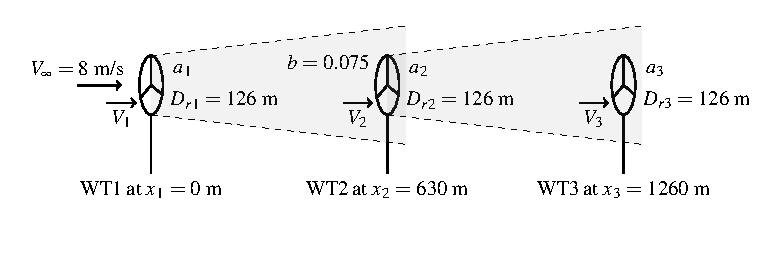
\includegraphics[width=0.8\textwidth,trim={0.5cm 1.3cm 0.2cm 0.3cm},clip]{figures/figDirETC/testAICPark.pdf}
\caption{Schematic visualization of AIC wind farm optimization, adapted from \cite{barreiro2019data}.}
\label{figWindfarmAIC}
\end{figure}
%
The farm power $P_{\text{WF}}(\bm{a_{n_{\text{WT}}}})=\sum\limits_{i=1}^{n_{\text{WT}}}P_i(a_i)$ can be optimized by adjusting the axial induction factors of all turbines. This is done by inserting Equations~\eqref{eqcP_from_a} and \eqref{eqVri} into Equation~\eqref{eqPAIC}. 

Note that the Jensen model assumes all turbines are facing the wind and is therefore not suitable for calculating wake effects of turbines with intentional yaw misalignment, as used in wake redirection control (WRC). For this, the Bastankhah Gaussian wake model is used.

\subsubsection{Bastankhah Gaussian Model for Turbines with Yaw Misalignment}\label{secBastankhah}
In static Wake Redirection Control (WRC), the wake is steered away from downstream turbines by tilting or yawing the upstream turbines \cite{fleming14wakeeval}. A widely used analytical closed-form model for the wind speed deficits of a downstream turbine was developed and validated against wind tunnel data in \cite{bastankhah2016experimental}. The equations from this study are provided below for completeness.

Figure \ref{figWindfarmWRC} provides a two-dimensional schematic plot of the three-dimensional WRC setup for an array of three turbines.
%
\begin{figure}[ht]
\center
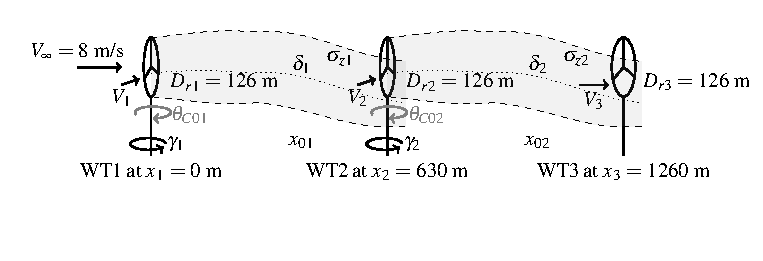
\includegraphics[width=0.8\textwidth,trim={0.5cm 1.3cm 0.2cm 0.3cm},clip]{figures/figDirETC/testWRCGaussiank.pdf}
\caption{Schematic visualization of WRC wind farm optimization, adapted from \cite{bastankhah2016experimental}.}
\label{figWindfarmWRC}
\end{figure}
%
The wake angle at the rotor, $\theta_{C0i}$, and the beginning of the far-wake region, $x_{0i}$, for which the model is shown to yield accurate results, are calculated using the approximation of the thrust coefficient $c_T$ from the axial induction factor $a_i$ and turbine yaw angle $\gamma_i$:
\[
c_T \approx 4a_i(1-a_i\cos(\gamma_i)).
\]
The wake angle $\theta_{C0i}$ at the rotor is given by:
\[
\theta_{C0i} =\frac{0.3\gamma_i}{\cos(\gamma_i)}(1-\sqrt{1-c_T\cos(\gamma_i) }).
\]
The start of the far-wake region $x_{0i}$ is computed as:
\[
\frac{x_{0i} }{D_r}=\frac{\cos(\gamma_i)(1+\sqrt{1-c_T })}{\sqrt{2}\left\lbrack k_{\alpha^*} I_i + k_{\beta^*} (1-\sqrt{1-c_T })\right\rbrack } 
\]
with coefficients $k_{\alpha^*}= 2.32 $ and $k_{\beta^*} = 0.154$ from \cite{bastankhah2016experimental}. The local turbulence intensity at hub height $z_h$ in front of the turbine, $I_i$, is defined as the ratio of wind speed fluctuations to the mean wind speed.
The wake deflection centerline $\delta_i$ for the far-wake region with $x > x_{0i}$ is given as:
\[
\frac{\delta_i}{D_r} =\theta_{C0i} \frac{x_{0i}}{D_r}  + \frac{\theta_{C0i}}{14.7} \sqrt{\frac{\cos(\gamma_i)}{b_y b_z c_T}} (2.9 +1.3\sqrt{1-c_T}-c_T)K_{\text{ln}}
\]
with:
\[
K_{\text{ln}}= \ln\left( \frac{(1+\sqrt{c_T })(1.6\sqrt{\frac{8\sigma_{yi}\sigma_{zi}}{D_r^{2} \cos(\gamma_i)}}-\sqrt{c_T })}{(1-\sqrt{c_T })(1.6\sqrt{\frac{8{\sigma_{yi} \sigma_{zi}}}{D_r^{2} \cos(\gamma_i) }}+\sqrt{c_T })} \right)
\]
and wake expansion coefficients $b_y$ and $b_z$ for lateral and vertical wake expansions. The wake expansions $\sigma_{yi}$ and $\sigma_{zi}$ are:
\[
\frac{\sigma_{yi} }{D_r}=b_y \frac{(x-x_{0i} )}{D_r}+\frac{\cos(\gamma_i)}{\sqrt{8}}, \quad
\frac{\sigma_{zi}}{D_r}=b_z\frac{(x-x_{0i} )}{D_r}+\frac{1}{\sqrt{8}}.
\]
The far-wake velocity deficit, and consequently the wind speed at a downstream turbine, is calculated using the Gaussian wake model:
\[
V_i = V_{i-1}(1 - (1- K_C)e^{-0.5((y-\delta_i)/\sigma_{yi})^2} e^{-0.5((z-z_h)/\sigma_{zi})^2})
\]
where:
\[
K_C = \sqrt{1-\frac{c_T \cos(\gamma_i)}{8(\sigma_{yi} \sigma_{zi}/D_r^2)}}
\]
and $V_0 = V_{\infty}$, meaning that for the first turbine, $V_1 = V_{\infty}$ due to the freestream wind acting on it, resulting in $K_C= 1$.
The turbine power output is then calculated as:
\[
P_i(\bm{a}_i,\bm{\gamma}_i) = \frac{1}{2} \rho_A A_r c_{P}(a_i,\gamma_i)(V_{i}(\bm{a}_{i-1},\bm{\gamma}_{i-1}) \cos(\gamma_i))^3
\]
where the power coefficient $c_P$ is given by:
\[
c_P(a_i,\gamma_i)  \approx 4a_i(1-a_i\cos(\gamma_i))^2.
\]
%
The results from the Gaussian wake model are compared to those obtained from $\text{WFSim}$, which is based on a linearized form of the $\text{Navier-Stokes equations (NSE)}$. While the Gaussian model offers computational speed, it relies on empirical parameters and cannot capture complex, dynamic flow phenomena like wake-wake interaction or pressure effects. Therefore, to achieve higher fidelity while maintaining a feasible computational cost for control design, the simulation environment $\text{WFSim}$ is employed. An overview of the control-oriented $\text{NSEs}$ on which this simulator is based is provided in the next subsection.

\subsubsection{Navier-Stokes Equations (NSE)}
The fluid dynamics of the turbine wake, affecting air pressure and wind speed, are fundamentally described by the NSE. In their two-dimensional, incompressible form, considering only the longitudinal and lateral velocity components and neglecting the vertical component, the equations governing the momentum and mass conservation are given as \cite{boersma2018control}:
\begin{align*}
\underbrace{
\begin{bmatrix}
\frac{\partial v_x}{\partial t} \\[1mm]
\frac{\partial v_y}{\partial t}
\end{bmatrix}
}_{\text{local acceleration}}
+
\underbrace{
\begin{bmatrix}
v_x \frac{\partial v_x}{\partial x} + v_y \frac{\partial v_x}{\partial y} \\[1mm]
v_x \frac{\partial v_y}{\partial x} + v_y \frac{\partial v_y}{\partial y}
\end{bmatrix}
}_{\text{convective term}}
+
\underbrace{
\begin{bmatrix}
\frac{\partial p}{\partial x} \\[1mm]
\frac{\partial p}{\partial y}
\end{bmatrix}
}_{\text{pressure gradient}}
+
\underbrace{
\begin{bmatrix}
\frac{\partial \tau_{xx}}{\partial x} + \frac{\partial \tau_{xy}}{\partial y} \\[1mm]
\frac{\partial \tau_{yx}}{\partial x} + \frac{\partial \tau_{yy}}{\partial y}
\end{bmatrix}
}_{\text{subgrid stress divergence}}
-
\underbrace{
\begin{bmatrix}
f_x \\[1mm]
f_y
\end{bmatrix}
}_{\text{turbine forcing}}
&= 
\begin{bmatrix} 0 \\ 0 \end{bmatrix}, \\[2mm]
\underbrace{\frac{\partial v_x}{\partial x} + \frac{\partial v_y}{\partial y}}_{\text{mass conservation / incompressibility}} &=   -\frac{\partial v_y}{\partial y}
\end{align*}
with $v_x$ and $v_y$ as wind components in the longitudinal $x$ and lateral $y$ directions, respectively, air pressure $p$, stress components $\tau_{xx}$, $\tau_{xy}$, $\tau_{yx}$ and $\tau_{yy}$, and turbine thrust $f_x$ and $f_y$. The four subgrid stress components $\tau_{ij}$ are the normal and shear stresses, where the first index indicates the direction of the momentum affected and the second index is the direction of the gradient causing the stress. The seemingly counter-intuitive second equation arises because the model must account for air passing over the turbine area rather than being forced to entirely circumvent it. The dimension reduction from the 3D equations, where longitudinal, lateral, and vertical velocity gradients sum to zero, is modeled in \cite{boersma2018control} via the approximation $\partial v_y/\partial y = \partial v_z/\partial z$. This approximation enables WFSim to avoid the so called blockage-effect typical of 2D models.
%
For compactness, these equations can be expressed in vector form as
\begin{align} \label{eq:NSE2d}
\frac{\partial \bm{v}}{\partial t}+ (\bm{v}\cdot \nabla_H)\bm{v} + \nabla_H p + \nabla_H\cdot\bm{\tau}_h  - \bm{f} = \bm{0}_{2\times1},\quad  
\nabla_H\cdot \bm{v} = -\frac{\partial v_y}{\partial y}
\end{align}
where:
\begin{itemize}
\item $\bm{v} =[v_x\;\;v_y]^T$ represents the wind speed vector.
\item The term $\frac{\partial \bm{v}}{\partial t}$ denotes the local acceleration of the wind flow over time.
\item The term $\nabla_H = [\frac{\partial}{\partial x}\;\;\frac{\partial}{\partial y}]^T$ is the gradient operator in the 2D simulation plane. Thus, the convective term $(\bm{v}\cdot \nabla_H)\bm{v}$ is the advection of momentum due to the wind's motion, describing how the local wind speed changes due to the motion of surrounding air.
\item The pressure gradient term, $\nabla_H p$, describes the force exerted on a fluid element due to differences in static pressure across that element.
\item The subgrid stress tensor $\boldsymbol{\tau}_h$ provides the effect of turbulence with
\[
\boldsymbol{\tau}_h =
\begin{bmatrix}
\tau_{xx} & \tau_{xy} \\
\tau_{yx} & \tau_{yy}
\end{bmatrix}.
\]
\item The term $\bm{f}$ represents the force exerted by turbines on the airflow, modeling the effect of energy extraction.
\item The divergence term $\nabla_H\cdot \bm{v} = - \frac{\partial v_y}{\partial y}$ enforces the incompressibility condition, ensuring mass conservation in the 2D flow field.
\end{itemize}
%
In WFSim, the NSEs are discretized in space using the finite volume method on a staggered 2D grid \cite{boersma2018control}. Figure~\ref{fig:9TurbMesh} shows the two overlapping grids, a primary mesh, depicted in blue, for the calculation of the wind speed components and a secondary mesh, visualized in gray, used for the calculation of the pressure components. 
\begin{figure}[h]
\centering
% \subfloat[Mesh wind field with turbines]{\includegraphics[width=0.50\textwidth]{figDirETC/Mesh9Turb.eps}}\hspace{0.02\textwidth}
% \subfloat[Zoom wind field corner]{\includegraphics[width=0.46\textwidth]{figDirETC/Mesh9TurbZoomNoLeg.eps}}
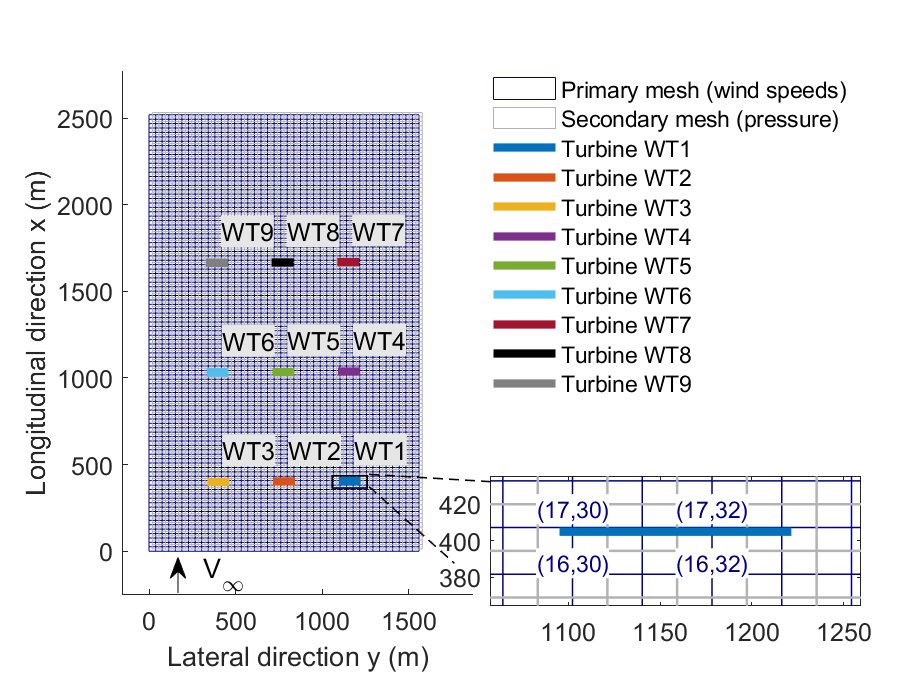
\includegraphics[width=0.85\textwidth,trim={0 0cm 0cm 0.0cm},clip]{figures/figDirETC/gridmesh9_tex.eps}
\caption[WFSim mesh setup for a nine-turbine wind farm.]{WFSim mesh setup for a nine-turbine wind farm. The primary mesh (blue) is used for wind speed calculations, and the secondary mesh (gray) for pressure. Turbines are shown as colored bars. Zoomed-in area around WT1 shows primary grid point indices.} 
\label{fig:9TurbMesh}
\end{figure}
The turbine locations for the default nine-turbine wind farm layout included with WFSim are depicted as bold, colored lines. The figure shows the entire wind field area and highlights a zoom around the first turbine, showing that the nodes of the secondary grid correspond to the centers of the primary grid cells and providing the index pair of the node as blue numbers. The effective wind speeds of the turbines is calculated based on the wind speeds at the nodes of the primary grid in front of the turbines. In the example in Figure~\ref{fig:9TurbMesh} these grid points leveraged for upstream wind turbine WT1 are the points in the 16$^{\text{th}}$ row from the 30$^{\text{th}}$ to the 33$^{\text{rd}}$ column. For better readability, only every second mesh point is annotated with the corresponding grid index in the zoom on the turbine location.

The finite volume method discretizes Partial Differential Equations (PDEs) such as the NSE by integrating them over small control areas to ensure the conservation of fluxes, such as the air mass flowing through the wind farm, across cell boundaries. In the WFSim 2D simulation, pressure is stored at the center of each grid cell, corresponding to the mesh points of the secondary mesh, while the longitudinal wind speed $v_x$, acting in vertical direction, is stored at the top and bottom edges and the lateral wind speed $v_y$ is stored at the left and right edges of the primary mesh.

In CFD software, the convective terms from Equation~\eqref{eq:NSE2d} are approximated with a combination of differencing schemes. These schemes compute how the wind carries momentum across the grid by switching between approaches to balance numerical stability and solution accuracy. Upstream differencing, which is more stable, is used when wind speeds are high, whereas central differencing, which is more accurate, is employed when wind speeds are low. Temporal discretization is performed using an implicit Euler method.

Numerical cost varies considerably with grid resolution, timestep, and available computing resources; for example, NREL's SOWFA documentation \cite{churchfield2012overview} reports a coarse LES example that ran at approximately 1.6\,s of wall-clock time per 1\,s of simulated time on 32 cores. Wall-clock time is the total real-world time elapsed from the start to the end of a simulation, including computation, inter-processor communication, disk I/O, memory access, and any idle or waiting time.

In \cite{boersma2018control}, which introduces the WFSim software, a mean computation time of approximately 0.02\,s per 1\,s timestep is reported on a single-core Intel~i7 platform instead on a server cluster. While no direct wall-clock time comparison with SOWFA is provided, the paper notes that high-fidelity LES solvers such as SOWFA require orders-of-magnitude longer runtimes and substantially more computational resources. In a two-turbine test case, WFSim was shown to reproduce the center-line mean wake velocity and power output time series from SOWFA reasonably well.

In WFSim, the wind field is approximated by a linear system for the velocity and pressure fields at each timestep, resulting in a significant reduction in simulation time and required computing resources. A more detailed overview of WFSim, including equations, is provided in Section~\ref{sec:WindFarmSimulationWFSim}, which also discusses the modifications made to WFSim to obtain the simulation results in \cite{dittmer2022data,dittmer2023koopman}.

\subsection{Wind Farm Control}\label{Subsection:Windfarmcontrol}
In this thesis, WFSim is used as a proof of concept for applying Koopman models to wind farm control, as it natively includes a farm-level controller that manages both turbine yaw $\gamma$ and thrust control $C_T^{\prime}$. The thrust controls, controlling the energy amount harvested by a turbine, are fictitious inputs used as substitutes for generator torque and blade pitch to avoid the need for a complex turbine model.

For closed-loop wind farm control, turbine control inputs are set to minimize the power reference tracking error and actuator activity, given a wind farm layout, a power grid reference $P_{\text{ref}}$, and the freestream wind speed $V_{\infty}$. Figure \ref{figBlockDiagramFarm} presents a block diagram of the control strategy for a wind farm consisting of two wind turbines.

\begin{figure}[ht]
\centering
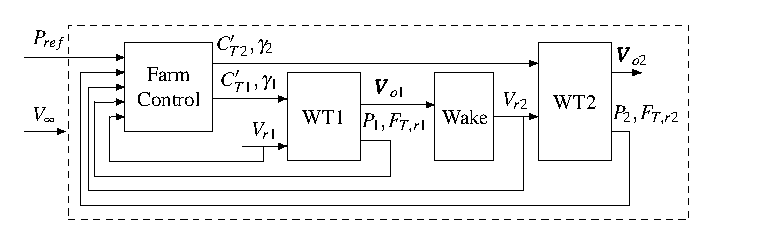
\includegraphics[width=0.8\textwidth,trim={0 0cm 0cm 0.3cm},clip]{figures/figDirETC/farmCtrl10_PandUr.pdf}
\caption{Block diagram of closed-loop wind farm control in WFSim}
\label{figBlockDiagramFarm}
\end{figure}

The wind farm layout and turbine parameters used in this study are consistent with those in \cite{sharan2022Koopman}, \cite{dittmer2022data}, and \cite{dittmer2023koopman}, upon which this thesis is based. The thrust control, which governs the amount of energy harvested by a turbine, is modeled as a fictitious input that substitutes for generator torque and blade pitch. This simplification eliminates the need for a detailed turbine model.

In the MPC implementation included with WFSim, it is assumed that the effective wind speeds at both turbines, $V_{r1}$ and $V_{r2}$, can be measured. These wind speeds, along with the power outputs $P_1$ and $P_2$, and the thrust forces $F_{T,r1}$ and $F_{T,r2}$, serve as feedback for the wind farm controller.

The effective wind speed $V_{ri}$ at the $i^{\text{th}}$ turbine is calculated as the root mean square of the wind speeds across the $n_r$ rotor segments:

\begin{align} \label{eqEffWindSpdWT}
V_{ri}(\gamma_{i}) &= \cos(\gamma_{i}) \sqrt{\frac{1}{n_r} \sum_{j = 1}^{n_r} V_{lj}^2},  
\quad  V_{lj}^2 = v_{xlj}^2 + v_{ylj}^2,
\end{align}
where $v_{xlj}$ and $v_{ylj}$ are the wind speed components in the $x$ and $y$ directions, respectively, at the $(l,j)$ grid point in the simulated WFSim domain. The vectors of wind speeds at the grid points directly behind the two turbines are denoted by $\bm{V}_{o1}$ and $\bm{V}_{o2}$.

Since the effective wind speed $V_{r2}$ is influenced by the wake of the first turbine, propagating through the wind speeds contained in $\bm{V}_{o1}$, the power and thrust output of the second turbine are also affected by the control input of the first turbine. 

The WFSim MPC discrete-time turbine model is given by:
\begin{align} \label{eqPowerWT}
\begin{split}
P_{i}(k+1) &= (1 - \tau) P_{i}(k) + \tau \frac{1}{2} \rho_a A_r \left(V_{ri}(\gamma_{i}(k))\right)^3 C_{Ti}^\prime(k), \\
F_{T,ri}(k+1) &= (1 - \tau) F_{T,ri}(k) + \tau \frac{1}{2} \rho_a A_r \left(V_{ri}(\gamma_{i}(k))\right)^2 C_{Ti}^\prime(k), \\
\hat{C}_{Ti}^\prime(k+1) &= (1 - \tau) \hat{C}_{Ti}^\prime(k) + \tau C_{Ti}^\prime(k),
\end{split}
\end{align}
with discrete sample time index $k$ and the constant $\tau$ as a discrete-time filter coefficient that determines the weighting between the current state and the new input at each time step. Larger values of  $\tau$ lead to faster updates. The state vector is defined as $\bm{x}_{\text{WT},i} = [P_i \;\; F_{T,ri} \;\; \hat{C}_{Ti}^\prime]^T$, where $P_i$ is the power and $F_{T,ri}$ is the thrust force of the $i^{\text{th}}$ turbine. The third state $\hat{C}_{Ti}^\prime$ is the filtered thrust control signal.

Equation~\eqref{eqPowerWT} is reformulated as
\begin{align} \label{eqWTWFSim}
\bm{x}_{\text{WT}i}(k+1) =\bm{A}_{\text{WT}i} \bm{x}_{\text{WT}i}(k) +\bm{B}_{\text{WT}i}(V_{ri}(\gamma_i))C_{Ti}^\prime(k), 
\end{align}
with the system and input matrices
\begin{align*}
\bm{A}_{\text{WTi}} = (1-\tau)\bm{I}_{3\times3},\text{ }\bm{B}_{\text{WTi}} = \tau[ C_P(V_{ri}(\gamma_i(k))) \quad C_F(V_{ri}(\gamma_i)) \quad 1]^T
\end{align*}
where $C_P(V_{ri}(\gamma_i)) = 1/2 \rho_a A_r (V_{ri}(\gamma_{i}))^3$ and $C_F(V_{ri}(\gamma_i)) = 1/2 \rho_a A_r (V_{ri}(\gamma_{i}))^2$ .
A concatenation into a wind farm model, with wind vector $\bm{V_r}$ and thrust $\bm{C}_{T}^\prime$ and yaw $\bm{\gamma}$ of all turbines, gives 
\begin{align} \label{eqLinWF}
\bm{x}_{\text{WF}}(k+1) = \bm{A}_{\text{WF}} \bm{x}_{\text{WF}}(k) + \bm{B}_{\text{WF}}(\bm{V_r}(\bm{\gamma}(k))) \bm{C}_{T}^\prime (k).
\end{align}
It is defined by the block diagonal system and input matrices $\bm{A}_{\text{WF}} \in {\mathbb{R}}^{3n_{\text{WT}} \times 3n_{\text{WT}}}$ and $\bm{B}_{\text{WF}} \in {\mathbb{R}}^{3n_{\text{WT}} \times n_{\text{WT}}}$ with turbine system and input matrices on their diagonals, and farm state $\bm{x}_{\text{WF}} \in {\mathbb{R}}^{3n_{\text{WT}}}$ for a farm with $n_{\text{WT}}$ turbines.

The models presented in Equations~\eqref{eqWTWFSim} and \eqref{eqLinWF} form the foundation of the wind farm baseline MPC algorithm and the qLMPC presented in this thesis. The theoretical frameworks required to design and implement MPC algorithms are introduced in Section~\ref{sec:Control-Theoretic Background}.

\section{Control-Theoretic Background}\label{sec:Control-Theoretic Background}
The following sections introduce the two modeling frameworks applied in this thesis, where first-principle based qLPV models are used to model wind turbines and Koopman theory based data-driven models for wind farms. This is followed by the MPC framework applied to both turbines and farms.

\subsection{Quasi-Linear Parameter-Varying Models}
\label{sec:qLPVmodels}

As described above, wind turbine dynamics are characterized by nonlinearities due to aerodynamic and structural effects. To be able to leverage the existing extensive linear control and estimation frameworks, Linear Parameter-Varying (LPV) and its generalized form, quasi-LPV (qLPV), can be used to represent nonlinear dynamics through a linear structure with time-varying parameters \cite{hoffmann2014survey}. These scheduling parameters capture the nonlinearity while preserving computational efficiency and physical interpretability. In the context of wind energy conversion systems, qLPV modeling enables systematic controller design across the whole operating range of a turbine without requiring full nonlinear computations at each time step.

\subsubsection{Standard and Velocity-based qLPV Models}
\label{sec:qLPVmodelTheory}

In general, nonlinear continuous-time dynamics can be expressed as
\begin{align} \label{eq:stateSpaceGeneral}
    \dot{\bm{x}}(t) = \bm{f}(\bm{x}, \bm{w}), \quad
    \bm{y}(t) = \bm{h}(\bm{x}, \bm{w}),
\end{align}
with the state $\bm{x} \in \mathbb{R}^{n_x}$, input $\bm{w} \in \mathbb{R}^{n_w}$, and output $\bm{y} \in \mathbb{R}^{n_y}$. The functions $\bm{f}$ and $\bm{h}$ are nonlinear, but locally smooth in the neighborhood of operating points.

The matrices of the LPV model are the linearization of Equation~\eqref{eq:stateSpaceGeneral} around relevant operating points, yielding the Jacobian-based matrices
\begin{equation}\label{eq:contMatricesqLPV}
    \begin{aligned}
        \bm{A}_c(\bm{x},\bm{w}) &= \nabla_{\bm{x}} \bm{f}(\bm{x},\bm{w}) \in \mathbb{R}^{n_x \times n_x}, \quad
        \bm{B}_c(\bm{x},\bm{w}) = \nabla_{\bm{w}} \bm{f}(\bm{x},\bm{w}) \in \mathbb{R}^{n_x \times n_u}, \\
        \bm{C}_c(\bm{x},\bm{w}) &= \nabla_{\bm{x}} \bm{h}(\bm{x},\bm{w}) \in \mathbb{R}^{n_y \times n_x}, \quad
        \bm{D}_c(\bm{x},\bm{w}) = \nabla_{\bm{w}} \bm{h}(\bm{x},\bm{w})\in \mathbb{R}^{n_y \times n_u}.
    \end{aligned}
\end{equation}
The scheduling parameter vector $\bm{\rho}_\Rho$ is constructed from selected states and inputs, and the qLPV model becomes:
\begin{equation} \label{eq:standardqLPV1}
    \begin{aligned}
        \dot{\bm{x}}(t) &= \bm{A}_c(\bm{\rho}_\Rho) \bm{x}(t) + \bm{B}_c(\bm{\rho}_\Rho) \bm{w}(t), \\
        \bm{y}(t) &= \bm{C}_c(\bm{\rho}_\Rho) \bm{x}(t) + \bm{D}_c(\bm{\rho}_\Rho) \bm{w}(t). 
    \end{aligned}
\end{equation}
An alternative, velocity-based qLPV formulation considers the derivatives of state and input rather than the states and inputs themselves \cite{cisneros2016efficient}. Differentiating Equation~\eqref{eq:standardqLPV1} gives:
%\begin{equation}\label{eq:velocityForm}
\begin{align*}
    \ddot{\bm{x}}(t) &= \bm{A}_c(\bm{\rho}_\Rho) \dot{\bm{x}}(t) +\bm{B}_c(\bm{\rho}_\Rho) \dot{\bm{w}}(t), \\
    \dot{\bm{y}}(t) &= \bm{C}_c(\bm{\rho}_\Rho)  \dot{\bm{x}}(t) + \bm{D}_c(\bm{\rho}_\Rho) \dot{\bm{w}}(t).
\end{align*}
%\end{equation}
This velocity-based form has the advantage of steady-state behavior at the origin ($\dot{\bm{x}}=\dot{\bm{w}}=0$), eliminating the need to store equilibrium state and input vectors at each operating point. Therefore, no trimming calculations are required once a physical model is derived based on the nonlinear dynamics. 

The MPC implementations presented in this thesis are formulated in discrete time within a velocity-based qLPV framework. The matrices $\bm{A}_d\in \mathbb{R}^{n_x \times n_x}$ and $\bm{B}_d\in \mathbb{R}^{n_x \times n_u}$ of the discrete velocity form can be obtained via zero-order hold discretization from their continuous-time counterparts from Equation~\ref{eq:contMatricesqLPV}:
\begin{equation} \label{eq:zoh1}
    \begin{aligned}
        \bm{A}_d(\bm{\rho}_\Rho) &= e^{\bm{A}_c(\bm{\rho}_\Rho)T_s}, \\
        \bm{B}_d(\bm{\rho}_\Rho) &= \left( \int_0^{T_s} e^{\bm{A}_c(\bm{\rho}_\Rho)\tau} \, d\tau \right) \bm{B}_c(\bm{\rho}_\Rho),
    \end{aligned}
\end{equation}
with the sample time $T_s$. A velocity-based discrete state-space model can then be set up as:
\begin{align} \label{eq:velocityFormDisc}
    \Delta\bm{x}(k+1) = \bm{A}_d(\bm{\rho}_\Rho) \Delta\bm{x}(k) + \bm{B}_d(\bm{\rho}_\Rho) \Delta\bm{u}(k)
\end{align}
with $
\Delta\bm{x}(k) = \bm{x}(k) - \bm{x}(k-1) \text{ and } \Delta\bm{u}(k) = \bm{u}(k) - \bm{u}(k-1).$

A subset of states $\bm{x}_{\text{sel}} \in \mathbb{R}^{n_{\text{sel}}}$ is selected for explicit inclusion in the qLPV model's state vector, enabling direct constraints on these states within the MPC scheme. The discrete difference vector $\Delta\bm{x}(k)$ at time sample $k$ is augmented with the vector 
\begin{equation}  \label{eq:differenceSelectedFormDisc}
    \begin{aligned}
        \bm{x}_{\text{sel}}(k) &= \bm{x}_{\text{sel}}(k-1) + \Delta \bm{x}_{\text{sel}}(k) \\
        &=  \bm{x}_{\text{sel}}(k-1) +  \bm{A}_{d,\text{sel}}\Delta \bm{x}_{\text{sel}}(k-1) +  \bm{B}_{d,\text{sel}}\Delta \bm{u}_{\text{sel}}(k-1),        
    \end{aligned}
\end{equation}
with the matrices $\bm{A}_{d,\text{sel}} \in  \mathbb{R}^{n_{\text{sel}} \times n_x}$ and  $\bm{B}_{d,\text{sel}} \in  \mathbb{R}^{n_{\text{sel}} \times n_x}$ representing the rows of the state and input matrices corresponding to the selected states.
%
%
The resulting augmented state-space model with the expanded state vector $\bm{x}_{\text{ext}} =[\bm{x}_{\text{sel}}^T \; \; \Delta\bm{x}^T ]^T$ is derived based on the matrices used in Equation~\eqref{eq:velocityFormDisc} and ~\eqref{eq:differenceSelectedFormDisc}:
\begin{equation}\label{eq:discreteVelocityqLPV}
    \begin{aligned}
        \begin{bmatrix} \bm{x}_{\text{sel}}(k+1) \\ \Delta\bm{x}(k+1) \end{bmatrix} 
        &= \begin{bmatrix} \bm{I}_{n_{\text{sel}}} & \bm{A}_{d,\text{sel}}(\bm{\rho}_\Rho) \\ 
            \bm{0}_{n_x \times n_\text{sel}} & \bm{A}_d(\bm{\rho}_\Rho) 
        \end{bmatrix}
        \begin{bmatrix} \bm{x}_{\text{sel}}(k) \\ \Delta\bm{x}(k) \end{bmatrix}
        + \begin{bmatrix} \bm{B}_{d,\text{sel}}(\bm{\rho}_\Rho) \\ \bm{B}_d(\bm{\rho}_\Rho) \end{bmatrix} \Delta\bm{u}(k), \\
        y(k) &= \bm{x}_{\text{sel}}(k) = \begin{bmatrix} \bm{I}_{n_{\text{sel}}} & \bm{0}_{n_\text{sel} \times n_x} \end{bmatrix} 
        \begin{bmatrix} \bm{x}_{\text{sel}}(k) \\ \Delta\bm{x}(k) \end{bmatrix},
    \end{aligned}
\end{equation}
where both the selected states and the discrete differences of all states appear explicitly in the dynamics. 

This structured state expansion, necessary for velocity-based qLPV models used in constrained MPC algorithms, increases, and may even double, the state dimension. This complicates stability analysis and controller synthesis using robustness guarantees such as Linear Matrix Inequality (LMI) schemes. However, for the low-order MPC implementation presented here, the increased state dimension is not critical, and LMI-based robustness guarantees are not pursued.

If the scheduling parameter $\bm{\rho}_\Rho$ depends solely on exogenous variables (i.e., inputs and parameters), the system is strictly LPV. However, if $\bm{\rho}_\Rho$ depends additionally or purely on endogenous variables (i.e., system states), as in the wind turbine models discussed here, the resulting structure is a qLPV model. This distinction is important as the dependence on model states introduces implicit dependencies that must be accounted for during control design. Concretely in the case of qLPV models used for MPC, the scheduling parameter has to be fixed to specific values for all samples of the prediction horizon to calculate the prediction trajectory in dependence of the states, see~\cite{cisneros2016efficient}.

The qLPV framework approximates nonlinear dynamic systems by allowing the model matrices to vary smoothly over the operating range. This can be achieved in several ways, for example through precomputed local linearizations, data-driven identification, or first-principles models combined with physics-based lookup tables. In this work, a combination of first-principles models and physics-based lookup tables is used.


\subsubsection{qLPV Models based on BEM Models and Actuator Disk Models}
\label{sec:quasi-LPVTurbineModel}

For wind energy applications, the mapping from the disturbance input wind speed and the control inputs generator torque and pitch angle to turbine states, including, e.g., rotor speed and tower displacement, is obtained from the mathematical representations of wind turbine physics described in Section~\ref{windTurbineModel}. For a wind turbine model, two-dimensional lookup tables for thrust and torque, dependent on blade pitch, wind speed, and rotor speed, are derived from BEM models implemented in the FAST software. When these nonlinear aerodynamic relationships are combined with linearized tower and drivetrain dynamics, the overall model becomes a nonlinear ODE system that can be approximated locally as linear around each operating point. For the BEM-based turbine model, the scheduling vector
\[
\bm{\rho}_{\Rho,\text{WT}} = [V_\infty \quad \omega_r \quad \beta]^T, 
\]
which is based on wind speed, rotor speed, and blade pitch angle, represents the variations in aerodynamics. The qLPV matrices thus reflect that changes in these three parameters immediately shift the effective aerodynamic of the turbine. Chapter \ref{sec:WindTurbineqLPVModels} provides a detailed derivation of two qLPV wind turbine models, both based on lookup tables for thrust and torque coefficients generated using FAST. 

For farm level control, the actuator disk model provided in Section~\ref{windTurbineModel} includes the effective inflow wind speed of all turbines as a scheduling variable for all $n_{\text{WT}}$ wind turbines of a farm
\[
\bm{\rho}_{\Rho,\text{WF}} = [V_{r,1} \quad V_{r,2} \quad \ldots \quad V_{r,n_{\text{WT}}} ]^T. 
\]
This effective wind speed depends on both exogenous variables (ambient turbulence, upstream wakes) and endogenous system states (thrust and yaw angle of the turbines). Consequently, the scheduling map becomes partially state-dependent which is the defining feature of a qLPV model. 

By combining these qLPV representations with predictive control formulations, one can design MPC controllers that explicitly accommodate nonlinear aerodynamic effects while maintaining convex optimization structure. The qLPV wind farm model used in the MPC formulation implemented in WFSim (see Section~2.3.2) is a representative example.

\subsection{Koopman Theory for System Modeling} \label{sec:Koopman}

This section presents the principle of Koopman operators, followed by a description of the design of the Koopman matrix as a prediction scheme based on Koopman operators. The Koopman framework allows the representation of any finite-dimensional nonlinear system as an infinite-dimensional linear system. Extended Dynamic Mode Decomposition (EDMD) and Extended Input-Output DMD (EIODMD) are used in this work for finite matrix approximations of the infinite-dimensional Koopman operator. This thesis leverages notations and methods from \cite{arbabi2018data}, where a data-driven Koopman MPC framework for nonlinear PDEs was presented. The approach identifies a Koopman-linear model via EDMD to design a feedback controller, demonstrated on Burgers’ equation and NSE cavity flow. The latter example is particularly relevant to wind farm control, as both are governed by NSEs.

\subsubsection{Koopman Operator and Matrix}\label{KoopmanOperator}

The Koopman operator $\mathcal{K}$ provides a framework for transforming finite-dimensional nonlinear dynamics into an infinite-dimensional linear system. By approximating this operator with a finite-dimensional representation, the tools of linear system analysis and control theory can be directly applied to nonlinear systems. This approach was originally proposed in \cite{koopman1931hamiltonian}. For its application to controls see, e.g.,\cite{proctor2018generalizing}, or \cite{kaiser2020data}.

Consider a time-invariant, discrete-time autonomous nonlinear dynamical system with state
$\bm{x} \in \mathbb{R}^{n_{x}}$ and function $F:\mathbb{R}^{n_{x}} \to \mathbb{R}^{n_{x}}$ at sample time $k$:
\begin{equation}
\bm{x}(k+1) = F(\bm{x}(k)). \label{eq:nonLinSysKoop}
\end{equation}
The Koopman framework uses the evolution of functions of the state, instead of the evolution of the state $\bm{x}$, to describe nonlinear dynamics as a linear dynamical system. The functions of the states are referred to as observables. The infinite-dimensional observable $g_\infty(\bm{x})$ belongs to a Hilbert space $\mathcal{H}$ \footnote{A Hilbert space generalizes the concept of the Euclidean space to possibly infinite dimensions \cite{korda2018linear}.}, creating an infinite-dimensional lifted state:
\begin{equation}
\bm{\varphi}_\infty(k) = g_\infty(\bm{x}(k)).
\end{equation}
The linear, infinite-dimensional Koopman operator $\mathcal{K}: \mathcal{H} \to \mathcal{H}$ is defined by its action on these observables, propagating them forward in time:
\begin{equation} \label{eq:KoopmanUnforced}
\bm{\varphi}_\infty(k+1) = (\mathcal{K}g_\infty)(\bm{x}(k)) = g_\infty(F(\bm{x}(k))) = g_\infty(\bm{x}(k+1)).
\end{equation}
Figure~\ref{fig:koopman-diagram} visualizes the concept of a Koopman operator applied to an unforced nonlinear system, as described in Equations~\eqref{eq:nonLinSysKoop} to \eqref{eq:KoopmanUnforced}
\begin{figure}[htb]
\centering
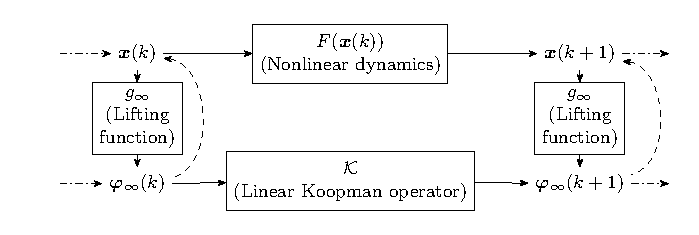
\includegraphics[width=0.82\textwidth, trim=0cm 0cm 0cm 0cm, clip]{figures/figuresBlockDiagram_IFAC23/KoopmanDiagram.pdf}
\caption{Block diagram of the nonlinear system, lifting function, and linear Koopman operator propagation for an unforced system (adapted from \cite{brunton2016koopman}).} 
\label{fig:koopman-diagram}
\end{figure}
The solid arrows show the main process flow. The dashed arcs indicate that the original states can be reconstructed from the lifted states and dash-dotted arrows represent the states' link to previous and future states.

Because the Koopman operator $\mathcal{K}$ is infinitely dimensional, it is generally impossible to use directly for real-time control calculations. This work hence employs a finite-dimensional approximation. A truncated lifting function $g: \mathbb{R}^{n_{x}} \to \mathbb{R}^{n_{g}}$ is used to create the approximated lifted state $\bm{\varphi} \in \mathbb{R}^{n_{g}}$:
\begin{equation}
\bm{\varphi}(k) = g(\bm{x}(k)). \label{eq:observ}
\end{equation}
By defining $g$ as a finite subset of $\mathcal{H}$, the operator $\mathcal{K}$ can be approximated by a finite-dimensional Koopman matrix $\hat{K}$. Note that in the following the truncated lifting functions and approximated lifted states are simply referred to as lifting function and lifted states, respectively, for better readability.

%
%Note that the finite function $g(\bm{x}(k))$ is an approximation of the observables $\g_\infty(\bm{x})$ which form a subset of an infinite-dimensional Hilbert space~$\mathcal{H}$, a complete vector space with an inner product that allows notions of length and angle to be defined. A Hilbert space generalizes the concept of the Euclidean space to possibly infinite dimensions \cite{korda2018linear}.% , providing a framework for analyzing functions and operators \cite{korda2018linear}.

%With lifting function $g$, the linear, infinite-dimensional Koopman operator $\mathcal{K}: \mathcal{H} \to \mathcal{H}$ for the nonlinear dynamical system is defined as
%\begin{equation} \label{eq:KoopmanUnforced}
%\bm{\varphi}(k+1) =(\mathcal{K}g)(\bm{x}(k)) = g(F(\bm{x}(k))) = g(\bm{x}(k+1)),
%\end{equation}
%where $\mathcal{K}$ propagates the observable $\bm{\varphi}(k) = g(\bm{x}(k))$ one time step forward. 


% Block diagram of the nonlinear system $F$, lifting function $g$, and linear Koopman operator $\mathcal{K}$ propagation for an unforced system (adapted from \cite{brunton2016koopman}).
% Block diagram of the Koopman operator framework. The top row depicts the nonlinear state evolution $F(\bm{x}(k))$, while the bottom row illustrates the linear evolution of the lifted observables $\boldsymbol{\varphi}(k)$ via the Koopman operator $\mathcal{K}$. 


This definition extends to nonlinear systems with input $\bm{w}$ as follows. The Koopman operator for controlled systems evolves on the extended state space $\mathbb{R}^{n_{x}} \times \ell(\mathcal{W})$, where $\ell(\mathcal{W})$ denotes the space of all infinite discrete input sequences $\bm{w} = (\bm{w}(k))_{k=1}^\infty$ \cite{arbabi2018data, korda2018linear}. The extended state vector 
\[
\bm{x}_w(k) = \begin{bmatrix} \bm{x}(k) \\ \bm{w}(k) \end{bmatrix} \in \mathbb{R}^{n_x + n_w}
\]
evolves according to the extended dynamics
\begin{align} \label{eq:KoopStateForced}
\bm{x}_w(k+1) = \tilde{F}_w(\bm{x}(k), \bm{w}(k)) = \begin{bmatrix} F_w(\bm{x}(k), \bm{w}(k)) \\ S(\bm{w}(k)) \end{bmatrix} = \begin{bmatrix} \bm{x}(k+1) \\ \bm{w}(k+1) \end{bmatrix},
\end{align}
where $F_w$ defines the state transition and the input sequence is moved forward by the shift operator $S$, defined by $S\left( (\bm{w}(k))_{k=1}^\infty \right) = (\bm{w}(k+1))_{k=1}^\infty$. The augmented flow map $\tilde{F}_w$ captures both the state transitions and the evolution of the exogenous signal.

The Koopman operator acts on the observables $\bm{\varphi}_w$ within the function space of the lifting function $g$. In practice, this infinite-dimensional operator is approximated by a finite-dimensional Koopman matrix 
\begin{align*}
\hat{\bm{K}} = [\bm{A}_K \;\; \bm{B}_K]
\end{align*}
This matrix maps the current extended lifted state to the next prediction:
\[
\bm{\varphi}(k+1) \approx \hat{\bm{K}} \bm{\varphi}_w(k) = [\bm{A}_K \;\; \bm{B}_K] \begin{bmatrix} \bm{\varphi}(k) \\ \bm{w}(k) \end{bmatrix},
\]
consistent with \cite{arbabi2018data, korda2018linear} and illustrated in Figure~\ref{fig:koopman-diagram-ext}. 
\begin{figure}[htbp]
\centering
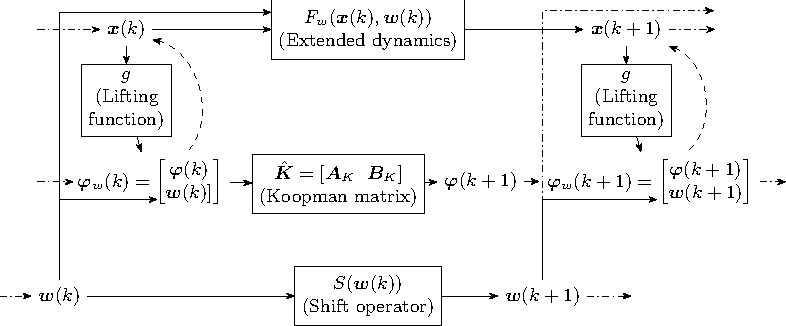
\includegraphics[width=0.95\textwidth, trim=0.cm 0.cm 0.cm 0cm, clip]{figures/figuresBlockDiagram_IFAC23/KoopmanDiagramExt.pdf}
\caption{Block diagram of the nonlinear system, approximated lifting function, shift operator, and Koopman matrix propagation for a forced system (adapted from \cite{proctor2018generalizing})}.
\label{fig:koopman-diagram-ext}
\end{figure}

This includes the extended state dynamics \(F_w\), the shift operator \(S\) acting on the input sequence, lifting functions \(g_w\) that map states and inputs to the extended, lifted observable space $\bm{\varphi}$, the Koopman matrix \(\hat{K}\) propagating lifted states and the lifted state at the next sample  $\bm{\varphi}(k+1)$ derived from the extended, lifted observable  $\bm{\varphi}_w(k)$. As before, dashed arrows indicate that the original states and inputs can be recovered from the lifted observables.

An illustrative example of lifting nonlinear dynamics into a higher-dimensional linear system is given in \cite{brunton2016koopman}. Consider the discrete-time nonlinear system
\begin{align} \label{eq:BruntonEx1}
x_1(k+1) &= \mu x_1(k), \\
x_2(k+1) &= \lambda x_2(k) - \lambda x_1^2(k) + u(k),
\end{align}
where \( x_1, x_2 \in \mathbb{R} \), \( \mu, \lambda \in \mathbb{R} \), and \( u \in \mathbb{R} \) is a scalar control input. The system is clearly nonlinear due to the \( x_1^2(k) \) term. By introducing a new observable \( \varphi(k) = x_1^2(k) \), the system can be rewritten as 
\begin{equation} \label{eq:BruntonEx2}
\varphi(k+1) = x_1^2(k+1) = \mu^2 x_1^2(k) = \mu^2 \varphi(k),
\end{equation}
which evolves linearly. Leveraging Equations~\eqref{eq:BruntonEx1} to~\eqref{eq:BruntonEx2} to stack the states and the observable into a lifted state vector, the dynamics can be expressed as a linear system:
\begin{equation}
\begin{bmatrix}
x_1(k+1) \\
x_2(k+1) \\
\varphi(k+1)
\end{bmatrix}
=
\begin{bmatrix}
\mu & 0 & 0 \\
0 & \lambda & -\lambda \\
0 & 0 & \mu^2
\end{bmatrix}
\begin{bmatrix}
x_1(k) \\
x_2(k) \\
\varphi(k)
\end{bmatrix}
+
\begin{bmatrix}
0 \\
1 \\
0
\end{bmatrix}
u(k).
\end{equation}
This construction yields a finite-dimensional linear representation of the original nonlinear system in lifted coordinates, where the Koopman operator corresponds to a matrix multiplication.

However, the Koopman operator cannot always be represented as a matrix multiplication. As shown in \cite{brunton2016koopman}, systems with multiple fixed points, periodic orbits, or attracting/repelling structures cannot be exactly represented by a finite-dimensional Koopman model, as  finite linear systems have a single equilibrium point only.
%In \cite{brunton2016koopman}, it is stated:
%\begin{quote}
%For any system with multiple fixed points, periodic orbits, or attracting/repelling structures, 
%there is no finite-dimensional Koopman invariant subspace that explicitly includes the state. 
%This follows from the fact that these systems cannot be topologically conjugate 
%to a finite-dimensional linear system with a single fixed point.
%\end{quote}
%In other words, any finite-dimensional linear system can only have one equilibrium point, 
%so it cannot exactly capture the behavior of more complex nonlinear systems.
As a discrete-time example where the Koopman operator is infinite-dimensional,  the scalar nonlinear system
\begin{equation}
x(k+1) = \mu x^2(k), \quad x \in \mathbb{R}, \ \mu \in \mathbb{R}
\end{equation}
is considered. Note that this system has two fixed points, concretely $x=0$ and $x=1/\mu$ for $\mu \neq 0$. The fixed point at the origin is attracting, since $f'(0)=0$, 
while the fixed point at $x=1/\mu$ is repelling, since $f'(1/\mu)=2$ with $|2|>1$. Defining the observable \( \varphi_1 = x^2 \) leads to
\begin{equation}
\varphi_1(k+1) = x^2(k+1) = (\mu x^2(k))^2 = \mu^2 x^4(k),
\end{equation}
which introduces the need for a new observable \( \varphi_2 = x^4 \). Continuing this process,
\begin{equation}
\varphi_2(k+1) = x^4(k+1) = (\mu x^2(k))^4 = \mu^4 x^8(k),
\end{equation}
and so on, yields an infinite sequence of new observables. Therefore, a finite-dimensional Koopman operator cannot capture the dynamics of this system. The lifted space is, in this example, infinite-dimensional.

In cases where the Koopman operator is infinite-dimensional, one approach is to approximate it with a finite matrix using a suitable set of observables. This Koopman matrix can be identified directly from data by DMD, without requiring a closed-form model of the underlying dynamics. This makes the approach applicable to wind farm control, where the flow and wake dynamics are governed by the Navier-Stokes equations, for which no general analytical solution is known and whose discretization yields a state dimension far too large for an analytical lifting.


\subsubsection{Koopman Matrix for Wind Farm Modeling}\label{KoopmanIdentification}

In this work, the system states of the MPC model used to calculate the optimal control inputs are the wind speeds acting on the turbines. For a qLMPC design, estimating the wind speeds based on a wind measurement in front of the upstream turbine, EDMD is used. For a linear Koopman MPC design, which uses an estimate of the power output of the turbines, EIODMD is applied.

The discrete-time nonlinear dynamical system can be extended by an output $\bm{y}$ as
\begin{equation}
\bm{x}(k+1) = F_w(\bm{x}(k), \bm{w}(k)), \quad 
\bm{y}(k) = G(\bm{x}(k), \bm{w}(k)) \label{eq:nonLinSys}
\end{equation}
with states $\bm{x} \in \mathbb{R}^{n_{x}}$, inputs $\bm{w} \in \mathbb{R}^{n_{w}}$, outputs $\bm{y} \in \mathbb{R}^{n_{y}}$, and nonlinear functions $F_w : \mathbb{R}^{n_{x}} \times \mathbb{R}^{n_{w}} \to \mathbb{R}^{n_{x}}$ and $G : \mathbb{R}^{n_{x}} \times \mathbb{R}^{n_{w}} \to \mathbb{R}^{n_{y}}$.


Lifting functions $g$ are defined as before as nonlinear combinations of the original states $\bm{x}$. In this work a new state $\bm{\varphi}\in\mathbb{R}^{n_{g}}$ is defined as a concatenation of the state $\bm{x}$ and the nonlinear combination of the states $g_{\varphi}$, i.e., the observables $\bm{\varphi}_g = g_{\varphi}(\bm{x})$, and hence $ \bm{\varphi} = g(\bm{x})$ with $\bm{\varphi}^T = [\bm{x}^T \; \bm{\varphi}_g^T]^T$.

A finite linear approximation of the nonlinear system given in Equation~\eqref{eq:nonLinSys} is:
\begin{align*}
\bm{\varphi}(k+1)=\bm{A}_{\hat{K}}\bm{\varphi}(k)+\bm{B}_{\hat{K}}\bm{w}(k), \quad 
\hat{\bm{y}}(k) = \bm{C}_{\hat{K}}\bm{\varphi}(k) + \bm{D}_{\hat{K}}\bm{w}(k),%\label{eq:linearPredictor}
\end{align*}
where $\hat{\bm{y}}$ is the vector of predicted output $\bm{y}$, $\bm{A}_{\hat{K}}\in \mathbb{R}^{{n_g}\times {n_g}}$, $\bm{B}_{\hat{K}}\in \mathbb{R}^{n_\varphi\times n_w}$, $\bm{C}_{\hat{K}}\in \mathbb{R}^{n_y\times n_\varphi}$, and $\bm{D}_{\hat{K}}\in \mathbb{R}^{n_y\times n_w}$.

For EIODMD, data from $n_o$ samples containing the measured state, input, and output vectors are collected and organized into two data matrices. The first matrix, $\bm{X}_{\text{EIODMD}}$, contains the state and input snapshots. The second matrix, $\bm{X}_{\text{EIODMD},+}$, contains the subsequent state snapshots and the corresponding outputs:
\begin{align} \label{eq:DataCollAIC}
\bm{X}_{\text{EIODMD}} &= \begin{bmatrix} 
\bm{x}(1) & \bm{x}(2) & \dots & \bm{x}(n_o-1) \\
\bm{w}(1) & \bm{w}(2) & \dots & \bm{w}(n_o-1)
\end{bmatrix} \in \mathbb{R}^{(n_x+n_w)\times (n_o-1)}, \\
\bm{X}_{\text{EIODMD},+} &= \begin{bmatrix} 
\bm{x}(2) & \bm{x}(3) & \dots & \bm{x}(n_o) \\
\bm{y}(1) & \bm{y}(2) & \dots & \bm{y}(n_o-1)
\end{bmatrix} \in \mathbb{R}^{(n_x+n_y)\times (n_o-1)}.
\end{align}
%
The matrices $\bm{A}_{\hat{K}}, \bm{B}_{\hat{K}}, \bm{C}_{\hat{K}}$, and $\bm{D}_{\hat{K}}$ can be obtained by solving the optimization problem:
\begin{equation}
\min_{\hat{K}} \sum_{k=1}^{n_{o}-1} \left\Vert \begin{bmatrix}
\bm{\varphi}(k+1)\\ \bm{y}(k)
\end{bmatrix} - \hat{K} \begin{bmatrix}
\bm{\varphi}(k)\\ \bm{w}(k)
\end{bmatrix} \right\Vert_{2}^{2} \label{eq:ApproxKalman}
\end{equation}
with the Koopman matrix defined as:
\begin{align*}
\hat{K} = \begin{bmatrix}
\bm{A}_{\hat{K}} & \bm{B}_{\hat{K}}\\ 
\bm{C}_{\hat{K}} & \bm{D}_{\hat{K}} 
\end{bmatrix} \in \mathbb{R}^{(n_g + n_y) \times (n_g + n_w)}.
\end{align*}
%
The lifting functions are applied to data from the matrices $\bm{X}_{\text{EIODMD}}$ and $\bm{X}_{\text{EIODMD},+}$ to construct two matrices containing these lifted states:
\begin{align}
\bm{L}_u &= \begin{bmatrix} 
\bm{\varphi}(1) & \cdots & \bm{\varphi}(n_{o}-1)\\
\bm{w}(1) & \cdots & \bm{w}(n_{o}-1) 
\end{bmatrix} \in \mathbb{R}^{(n_g + n_w) \times (n_o - 1)}, \\
\bm{L}_{+} &= \begin{bmatrix}
\bm{\varphi}(2) & \cdots & \bm{\varphi}(n_{o})\\
\bm{y}(1) & \cdots & \bm{y}(n_{o}-1)
\end{bmatrix} \in \mathbb{R}^{(n_g + n_y) \times (n_o - 1)}. \label{eq:Lplus}
\end{align}
%
The optimization problem \eqref{eq:ApproxKalman} is reformulated as:
\[
\min_{\hat{K}} \left\Vert \bm{L}_{+} - \hat{K} \bm{L}_u \right\Vert_{F}^{2},
\]
where \( \left\Vert \cdot \right\Vert_{F} \) denotes the Frobenius norm. The analytical solution to this linear least squares problem is:
\begin{align*}
\hat{K} = \bm{L}_{+} \bm{L}_u^{\dagger},
\end{align*}
where \( ^{\dagger} \) denotes the Moore–Penrose pseudoinverse. For EDMD, only the upper part of the Koopman matrix \( \hat{K} \), denoted as \( \hat{K}_u \), which contains the system and input matrices, is used:
\begin{align}
\hat{K}_u = \begin{bmatrix} \bm{A}_{\hat{K}} & \bm{B}_{\hat{K}} \end{bmatrix}.
\end{align}
This matrix can be derived from the following problem:
\begin{equation}
\min_{\hat{K}_u} \sum_{k=1}^{n_{o}-1} \left\Vert
\bm{\varphi}(k+1) - \hat{K}_u
\begin{bmatrix}
\bm{\varphi}(k)\\ \bm{w}_u(k)
\end{bmatrix}
\right\Vert_{2}^{2}
\label{eq:ApproxKalmanEDMD}
\end{equation}
with the corresponding solution:
\begin{align*}
\hat{K}_u = \bm{L}_{+,u} \bm{L}_u^{\dagger},
\end{align*}
where \( \bm{L}_{+,u} \) is the upper part of the matrix \( \bm{L}_{+} \), as defined in Equation~\eqref{eq:Lplus}, i.e., the concatenation of samples of the vector \( \bm{\varphi} \) at different time steps. The input is denoted \( \bm{w}_u \), as it differs from the input used for EIODMD.

Figure~\ref{fig:BlockEDMDEIODMD} shows the inputs and outputs of the EDMD and EIODMD models.
\begin{figure}[h]
\centering
\subfloat[EDMD]{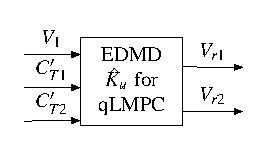
\includegraphics[width=0.35\textwidth]{figures/figuresBlockDiagram_IFAC23/farm1_OL2.pdf}}%
\hspace{0.05\textwidth}
\subfloat[EIODMD]{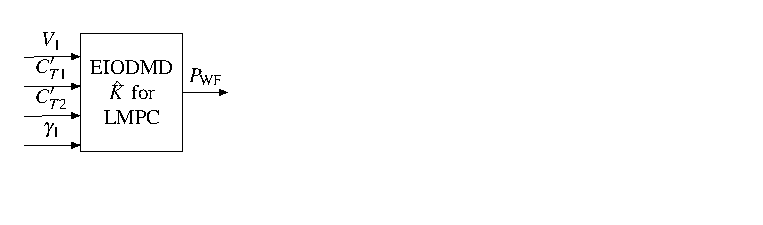
\includegraphics[width=0.35\textwidth, trim=0.0cm 1cm 8.5cm 0.5cm, clip]{figures/figuresBlockDiagram_IFAC23/EIODMD.pdf}}
\caption{Inputs and outputs of the EDMD and EIODMD models with lifted states $\bm{\varphi}$ based on effective wind speeds $V_{r1}$ and $V_{r2}$.}
\label{fig:BlockEDMDEIODMD}
\end{figure}

The states used to construct both models are the effective wind speeds acting on the turbines, specifically \( V_{r1} \) and \( V_{r2} \), along with lifted states derived from them. In this work, only polynomial functions are used, specifically the squares and cubes of the effective wind speeds, which correspond to aerodynamic force and power dependencies. The observable vector for both algorithms is:
\begin{align*}
\bm{\varphi} = [V_{r1} \quad V_{r2} \quad V^2_{r1} \quad V^2_{r2} \quad  V^3_{r1} \quad V^3_{r2}]^\top \in \mathbb{R}^6.
\end{align*}
For EDMD, the inputs include the thrust control inputs and the wind measurement taken in front of the first turbine. For EIODMD, the inputs include all those used in EDMD, as well as the yaw control input of the first turbine, since EIODMD is applied in a combined thrust and yaw control setting. Hence, the inputs are:
\begin{align*}
\bm{w}_{u} = [V_1 \quad C^{\prime}_{T1} \quad C^{\prime}_{T2}]^\top \in \mathbb{R}^3 \quad\text{and} \quad
\bm{w} = [V_1 \quad C^{\prime}_{T1} \quad C^{\prime}_{T2} \quad \gamma_1]^\top \in \mathbb{R}^4.
\end{align*}
The output of the EDMD model consists of the two states \( V_{r1} \) and \( V_{r2} \), whereas the output of the EIODMD model is the total wind farm power, i.e., the sum of the power outputs of both turbines.


While data-driven approaches such as EIODMD for Koopman MPC are particularly 
suitable for wind farm control, where complex wake interactions make first-principles 
modeling challenging, they may not be the optimal choice for individual wind turbines. 
The dynamics of a single turbine are well understood and can be accurately described 
using ODEs, making first principle-based control strategies more appropriate, with qLMPC being investigated in this work. 

%The following section explores the use of the qLPV framework, which leverages known turbine physics for efficient and reliable control design.

\subsection{Model Predictive Control}
Model Predictive Control (MPC) is an optimization-based control strategy that computes control inputs by repeatedly solving a finite-horizon optimal control problem online, see e.g. \cite{rawlings2017model} for a detailed description. At each discrete time step $k$, a sequence of future control inputs is determined by minimizing a cost function $J$ over a prediction horizon of $n_h$ steps, subject to the system dynamics and any state and input constraints. The general MPC problem takes the form:
\begin{align} \label{eqMPCGeneral}
    \begin{array}{l}
        \underset{\bm{U}(k)}{\text{min }} J(\bm{U}(k)) = \sum_{j=0}^{n_h - 1} \bm{x}(k+j)^T \bm{Q}\, \bm{x}(k+j) + \bm{u}(k+j)^T \bm{R}\, \bm{u}(k+j) \\
        \text{subject to } \bm{x}(k+j+1) = f(\bm{x}(k+j), \bm{u}(k+j)), \quad j \in \{0, 1, \dots, n_h-1\}
    \end{array}
\end{align}
where $\bm{x}$ and $\bm{u}$ denote the state and input vectors, $\bm{Q}$ and $\bm{R}$ are positive semi-definite weighting matrices penalizing state deviation and control effort, respectively. The vector $\bm{U}$ contains the values of the input vector at all samples of the prediction horizon and the vector $\bm{X}$ the corresponding state vectors:
\begin{align*}
     \bm{U}(k) &= \begin{bmatrix} \bm{u}(k)^T \quad \bm{u}(k+1)^T \quad \ldots \quad  \bm{u}(k+n_h-1)^T \end{bmatrix}^T \in \mathbb{R}^{n_h n_u \times 1},\\
      \bm{X}(k) &= \begin{bmatrix} \bm{x}(k)^T \quad \bm{x}(k+1)^T \quad \ldots \quad  \bm{x}(k+n_h-1)^T \end{bmatrix}^T \in \mathbb{R}^{n_h n_x \times 1}.
\end{align*}
%
 Only the first element of the optimal input sequence is applied, after which the horizon is shifted forward and the problem is solved again, following the receding horizon principle. Therefore, of the calculated values of the horizon only the first sample is directly used, but all values of the horizon of the current control input are stored to be used for a warm start in the next step.
 
The original formulation of MPC, as provided in Equation~\ref{eqMPCGeneral}, penalizes the amplitude of state and control values. The wind farm MPC controller, however, aims to minimize the power reference tracking error, instead of the states, as well as the actuator activity, instead of the actuator amplitude. Hence, the cost function $J$ is formulated based on the tracking error trajectory $\bm{E}(k)$ and the input trajectory $\Delta \bm{U}(k)$ for the $n_h$ sample steps of the prediction horizon:
\begin{align} \label{eqObjFun1}
    \begin{array}{l} 
        \underset{\bm{U}(k)}{\text{min }} J(\bm{U}(k)) = \bm{E}(k)^T \bm{Q}\bm{E}(k) +\Delta \bm{U}(k)^T \bm{R} \Delta \bm{U}(k) \\
        \text{subject to Equation } \eqref{eqLinWF}, \quad   k \in \{1, 2, \dots, n_h-1\}
    \end{array}
\end{align}
%
with the weighting matrices $\bm{Q}$ and $\bm{R}$. The trajectory of the farm power tracking error $\bm{E}$ is:
\begin{align*}
    \bm{E}(k) = \begin{bmatrix} e(k) & e(k+1) & \dots & e(k + n_h - 1) \end{bmatrix}^T \in \mathbb{R}^{n_h \times 1},
\end{align*}
where the power reference tracking error at time step $k$ on the farm level is calculated as 
\begin{align*}
    e(k) = P_{\text{ref}}(k) - P_{\text{WF}}(k). 
\end{align*}
%
The change in control inputs $\Delta \bm{U}$ is calculated as:
\begin{align*}
    \Delta \bm{U}(k) = \begin{bmatrix} \bm{u}(k) - \bm{u}(k-1) \\ \bm{u}(k+1) - \bm{u}(k) \\ \vdots \\ \bm{u}(k+n_h - 1) - \bm{u}(k + n_h - 2) \end{bmatrix} \in \mathbb{R}^{n_h n_u \times 1},
\end{align*}
with the vector $\bm{u}(k) \in \mathbb{R}^{n_u \times 1}$ containing all control inputs for all turbines at time~$k$.

This baseline MPC scheme is compared with Koopman-based MPC, i.e., an MPC based on a linear wind farm model derived using DMD. Koopman models are used to estimate the effective wind speeds rather than assuming that the measurements are available. To identify the Koopman models, known physical relationships of the NSEs are exploited when choosing the lifted states.

The next chapter describes in detail the set-up of two qLPV wind turbine models used for qLMPC for wind turbines. 

    \chapter{Wind Turbine qLPV Models} \label{sec:WindTurbineqLPVModels}
A wind turbine is a highly complex mechanical system. However, control-oriented models only aim to represent the dynamics that either provide information to the controller or are influenced by the actuator settings commanded by the controller. Therefore, the resulting models are of relatively low order. In Section  \ref{sec:MechanicalAerodynamicSubsystemModel}, the physical equations that serve as the basis for building a Simulink model of the turbine dynamics, and for the underlying models for the qLMPC algorithm discussed in the next chapter, are presented. The two first-principle models derived in this chapter are compared in Section \ref{sec:qLPVModelVerificationwithFAST0} in the time and frequency domains against the wind turbine simulation code FAST. The presented models have been published in \cite{dittmer2021velocity}.

\section{Nonlinear Models for qLMPC Design} \label{sec:MechanicalAerodynamicSubsystemModel}
Figure~\ref{fig:SchWTDefl} illustrates the movements and deflections of the tower and blades as a result of the forces and moments acting on them.
These structural deflections are associated with specific turbine modes, which represent distinct oscillations occurring at characteristic frequencies. Controllers are designed to dampen these modes to prevent excessive oscillations which may lead to fatigue loading and, in severe cases, dynamic instability and structural failure. If not properly controlled, these oscillations may resonate with the turbine’s natural frequencies, potentially causing harm to components or reducing its operational lifespan. Therefore, a mathematical model of the turbine must account for these modes to ensure accurate control and safe operation. 

Figure~\ref{fig:SchWTLPV} depicts the inputs, states, and geometric parameters utilized in the qLPV model of the wind turbine. Following the NREL 5MW documentation \cite{jonkman2009definition}, the tower-base coordinate system is defined with the x-axis pointing downwind, the y-axis transverse to the wind direction, and the z-axis vertical from tower base to yaw bearing. 
The blade coordinate system is defined according to the FAST documentation \cite{jonkman2005fast}: For each blade \(i = 1, 2, 3\), the axis definitions are as follows: the \(x_{bi}\)-axis is orthogonal to the \(y_{bi}\)- and \(z_{bi}\)-axes such that the three form a right-handed coordinate system, the \(y_{bi}\)-axis points toward the trailing edge of blade \(i\) and is parallel to the chord line at the zero-twist blade station, and the \(z_{bi}\)-axis points along the pitch axis toward the tip of blade \(i\). Consequently, the \(x_{bi}\)-axis denotes flapwise blade motion, the \(y_{bi}\)-axis edgewise motion, and torsion of the blade is defined as the rotation about the \(z_{bi}\)-axis. 

The geometric parameters depicted are the hub height $H_t$ and the rotor radius $R_r$. The model inputs are the rotor and generator torques, $T_r$ and $T_g$, as well as the rotor thrust $F_{T,r}$, which results from the wind acting on the wind turbine, $V_r$, which is perpendicular to its rotor. 
\begin{figure}[H]
    \centering
    \begin{minipage}[b]{11.5pc}
        \adjustbox{valign=b}{\includegraphics[width=11.5pc]{figuresBlockDiagram_IFAC23/windTurbineModesTwrBld01.pdf}}
        \caption{\label{fig:SchWTDefl}Schematic wind turbine diagram of tower and blade movements.}
    \end{minipage}
    \hspace{3pc}
    \begin{minipage}[b]{13.7pc}
        \adjustbox{valign=b}{\includegraphics[width=13.7pc]{figuresBlockDiagram_IFAC23/wind turbine 01.pdf}}
        \caption{\label{fig:SchWTLPV}Schematic LPV wind turbine model diagram with inputs, states, and parameters.}
    \end{minipage}
\end{figure}
%\noindent
Two qLPV designs are introduced in this section: the first models the rotor speed and the tower movement, while the second additionally accounts for the generator speed and the blade deflection. Both models use the three inputs rotor torque, generator torque, and thrust force.

The five states of the first model considered are the fore-aft and side-to-side tower deflections at hub height, $x_t$ and $y_t$, as well as their derivatives, $\dot{x}_t$ and $\dot{y}_t$, i.e., the fore-aft and side-to-side velocities, and the angular rotor speed $\omega_r$.
The state vector of the second model additionally contains the angular generator speed $\omega_g$ and the angular flapwise blade deflection $\delta_b$. Note that both the wind speed and the resulting force act in a distributed manner over the rotor disk. The vectors $V_r$ and $F_{T,r}$ give an equivalent one dimensional wind and force vector of the two dimensional wind field distributed over the rotor disk area and the forces acting at the segments of the blades.

 The thrust $F_{T,r}$ is the sum of the accumulated forces acting on the blades of the turbines, with the accumulated force per blade denoted $F_{T,bi}$ for the $i$th blade and with $n_b$ as the number of blades. To model the hub's movement and the resulting mechanical moments from the thrust force $F_{T,r}$, these forces are consolidated into a single force acting at a specific point on the blade, which is located at a distance $r_b$ from the rotor hub. This uses the same modeling as in \cite{Bianchi2007} where "the thrust forces distributed along each blade were
 replaced by a lumped force $F_T$ applied at a distance $r_b$ from the axis of rotation". 
In the following subsections, the underlying equations for two qLPV models are provided. Both turbine models share the drivetrain and actuator models, as well as the same aerodynamics model. The servo-elastic modeling of the first model is based on two simple physical equations governing the rotational motion and the tower bending. The more advanced servo-elastic modeling of the second model is derived from Lagrange's equation.

\subsection{Drivetrain, Torque Actuator, and Pitch Actuator Models}\label{subsec:drivetrain, Torque Actuator, and Pitch Actuator Models}
The flexible drivetrain subsystem, which contains a high-speed and a low-speed shaft, as well as a gearbox, transmits the aerodynamic torque to the generator. Linking multiple rigid bodies with flexible joints via a drivetrain results in a highly non-linear system, i.e., a system with dynamics that depend heavily on the operating point. However, for a control-oriented model, a system with one or two degrees of freedom in the rotational plane suffices, see, e.g., \cite{Bianchi2007}, \cite{peeters2006analysis} or  \cite{sharan2018actuator}.  
%
The drivetrain is modeled as a two-mass system, with the gearbox as a rigid body and the drivetrain's flexibility represented by a torsion spring on the low-speed shaft. The drivetrain dynamics are given by the following continuous first-order differential equations  \cite{sharan2018actuator}:
\begin{align} 
    J_{r}\dot{\omega_{r}}(t) &= T_{r}(t) - T_{\text{lss}}(t), \quad T_{\text{lss}}(t) = K_{s}\theta_{s}(t), \quad T_{\text{lss}}(t) = N_{g}T_{\text{hss}}(t), \nonumber\\
    J_{g}\dot{\omega_{g}}(t) &= \frac{1}{N_{g}} T_{\text{lss}}(t) - T_{g}(t), \quad \dot{\theta}_{s}(t) = \omega_{r}(t) - \frac{1}{N_{g}} \omega_{g}(t), \label{eq:DrvTr}
\end{align}
with angular rotor and generator speeds $\omega_{r}$ and $\omega_{g}$ and their respective torques $T_{r}$ and $T_{g}$. The low-speed and high-speed shaft torques are denoted by $T_{\text{lss}}$ and $T_{\text{hss}}$, while $J_{r}$ and $J_{g}$ represent the combined inertia on the rotor and generator sides, respectively. The torsion stiffness of the drivetrain is indicated by $K_{s}$, the gear ratio is given as $N_{g}$, and $\theta_{s}$ denotes the drivetrain's torsion angle. The torsional flexibility is neglected as the torsional mode lies above the frequency range of interest for power control. This allows the simplification $\dot{\omega}_g = N_g \dot{\omega}_r$ which results in
\begin{align} \label{eq:DrivetrainStiff}
     J_{g}N_g \dot{\omega}_r(t) = \frac{1}{N_{g}} T_{\text{lss}}(t) - T_{g}(t) \iff J_{g}N^2_g \dot{\omega}_r(t) = T_{\text{lss}}(t) - N_gT_{g}(t).
\end{align}
Combining Equation \eqref{eq:DrivetrainStiff} with the first equation from the Equations \eqref{eq:DrvTr} allows representing the rotor speed rate as
\begin{align*}
    \underbrace{(J_r + N^2_g J_g)}_{J_s}\dot{\omega}_r(t)= T_r(t) - N_g T_g(t)
\end{align*}
with the transmission inertia $J_s$. The extracted power $P_{g}$ is the product of the generator efficiency $\eta_{g}$ and the power $P_r$, i.e., the power extracted by the rotor from the available wind power $P_w$. It can be calculated as 
\begin{align}\label{eq:pg}
    P_{g}(t) = \eta_{g} T_{g}(t) \omega_{g}(t),
\end{align}
since equations \eqref{eq:DrvTr} show that the product of the rotor's angular speed and torque equals that of the generator in steady-state. Therefore, setting the torque of the generator directly influences the power output of the turbine.
%\noindent
%
The torque actuator can be regarded as the power conditioning unit of the turbine, and its dynamics can be modeled as a first-order differential equation \cite{odgaard2013fault}:
\begin{align}\label{eq:Tact}
    \dot{T}_{g}(t) = -\frac{1}{\kappa} T_{g}(t) + \frac{1}{\kappa} T_{g,\text{ref}}(t), 
\end{align}
where $\kappa$ denotes the torque actuator model parameter, and $T_{g,\text{ref}}$ is the reference generator torque.

Similarly, a first-order model with time constant $\tau$ is used in this work for the collective pitch $\beta_0$ of the three turbine blades:
\begin{align}\label{eq:betaact}
    \dot{\beta_0}(t) = -\frac{1}{\tau}\beta_0(t) + \frac{1}{\tau}\beta_{0,\text{ref}}(t).
\end{align}
Although the pitch system is often modeled as a second-order differential equation with natural frequency $\omega_{n,\beta}$ and damping ratio $\zeta_{\beta}$:
\begin{align*}
    \ddot{\beta_0}(t) = -2\zeta_{\beta_0} \omega_{n,\beta} \dot{\beta}_0(t) - {\omega_{n,\beta}}^2 \beta_0(t) + {\omega_{n,\beta}}^2 \beta_{0,\text{ref}}(t),
\end{align*}
the simplified representation as a first order system is made here since the relatively fast actuator dynamics have little influence on the investigated control objectives, which are consistent power output despite wind fluctuations and minimal tower movement. Note that the actuator dynamics, as provided in equations~\eqref{eq:Tact} and \eqref{eq:betaact}, result in low pass filtered signals of the commanded control output signals being applied to the turbine. However, the turbine dynamics, as modeled here in the aerodynamic and mechanical subsystem sections below, operate at much lower frequency and have greater impact on the power output as presented in equation~\eqref{eq:pg}.
\subsection{Aerodynamic Model}
The aerodynamic model represents the conversion of the available kinetic energy in the wind into mechanical energy using the rotor blades. Based on blade actuator disc theory, the mathematical equations for the rotor torque $T_{r}$, the aerodynamic power captured by the rotor $P_{r}$, and the thrust force $F_{T,r}$ can be derived from equations~\eqref{eq:PwPt} and~\eqref{eq:Ft}, used in Section~\ref{sec:WindTurbines} to provide the relationship between wind speed, thrust force and power, as
\begin{equation}\label{eq:aero}
    \begin{split}
        P_{r}(t) & = c_P(\lambda,\beta_0) P_{w}(t) = \frac{1}{2} \rho_a A_r c_P(\lambda,\beta_0) V_r(t)^3, \\
        T_{r}(t) & = \frac{P_{r}(t)}{\omega_{r}(t)} %= \frac{1}{2\omega_{r}(t)} \rho_a A_r c_P(\lambda,\beta_0) V_r(t)^3 \\
        = \frac{R_r}{2\lambda(t)} \rho_a A_r  c_P(\lambda,\beta_0) V_r(t)^{2} \\
        & =  \frac{1}{2} \rho_a R_r A_r  c_Q(\lambda,\beta_0) V_r(t)^{2} ,\\
        F_{T,r}(t) & = \frac{1}{2} \rho_a A_r  c_{T}(\lambda,\beta_0) V_r(t)^{2},
    \end{split}
\end{equation}
where the power, torque, and thrust coefficients $c_P$, $c_Q = c_P/\lambda$, and $c_{T}$ are functions of the blade pitch angle $\beta_0$ and the blade tip speed ratio $\lambda$, which is defined as
\begin{align*}
    \lambda(t) = \frac{\omega_{r}(t) R_r}{V_r(t)}
\end{align*}
and hence depends on the rotor radius $R_r$, the rotor angular speed $\omega_{r}$, and the effective wind speed $V_r$. The 2D matrices for the lookup tables of the power, torque and thrust coefficients, shown in Figure \ref{fig:CPCT}, are generated with the FASTTool.  Alternatively, they could be derived using steady-state FAST simulations with linear, equidistant sweeps of different wind speeds, rotor speeds, and pitch angles, where all input signals are kept constant. This has the advantage that the lookup tables can be designed for the exact version of FAST that is to be used in later calculations. However, as the simulations for the derivation and verification of the qLPV model in this thesis are exclusively done with FAST v8, the lookup tables are derived using functions available in the FASTTool.
%
\begin{figure} [h]
\centering
\subfloat[Power coefficient $c_P$]{%
    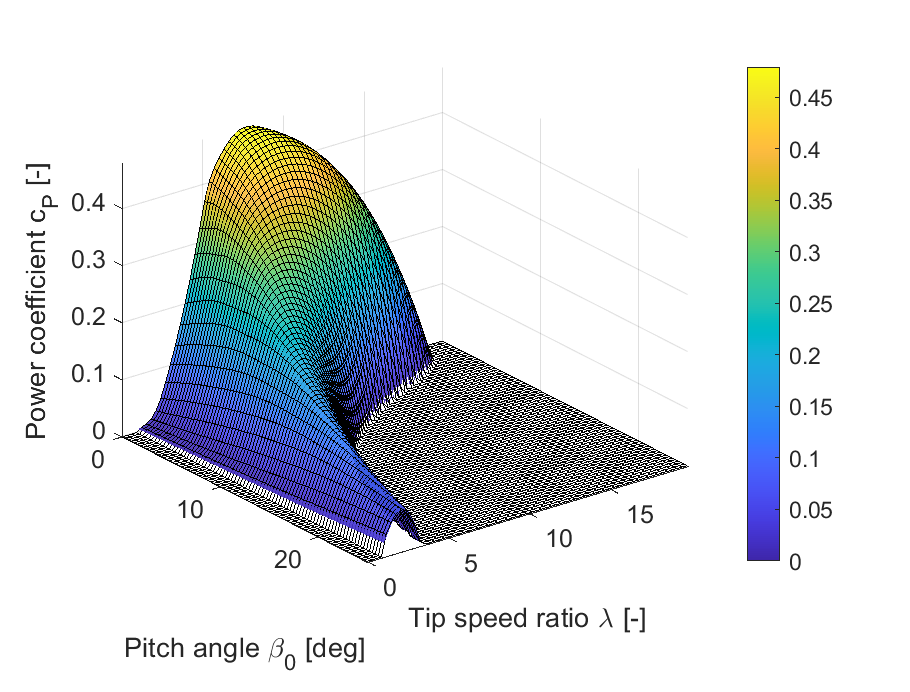
\includegraphics[width=0.49\textwidth]{figures/figDirECC21/Cp_NRRLFAST5MW.eps}
}\hfill
\subfloat[Torque coefficient $c_Q$]{%
    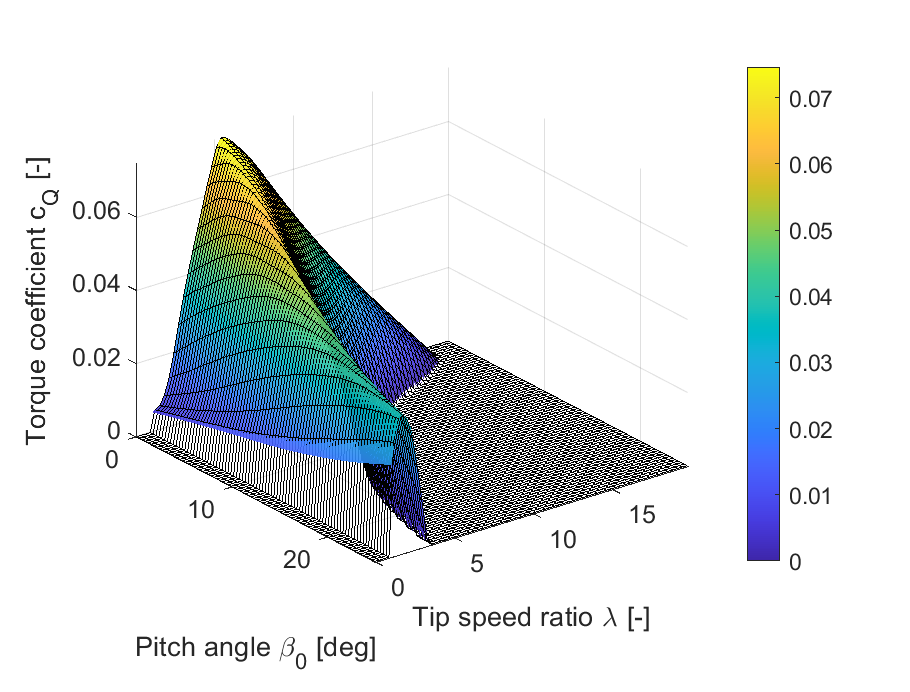
\includegraphics[width=0.49\textwidth]{figures/figDirECC21/Cq_NRRLFAST5MW.eps}
}\\[1ex]
\subfloat[Thrust coefficient $c_T$]{%
    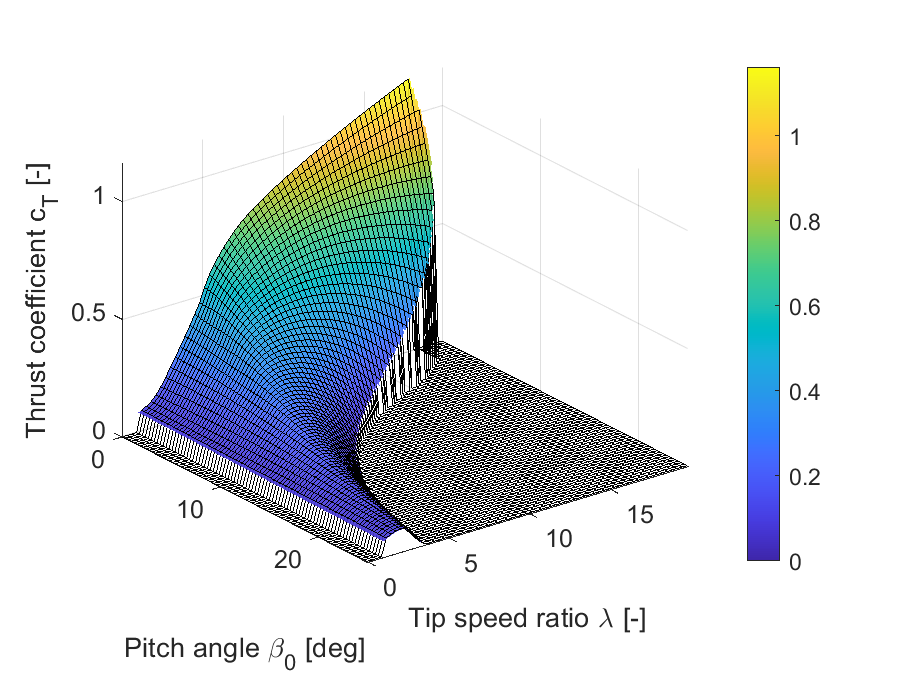
\includegraphics[width=0.49\textwidth]{figures/figDirECC21/Ct_NRRLFAST5MW.eps}
}
\caption{Lookup tables of power, torque and thrust coefficients with respect to blade pitch angle and tip speed ratio for the NREL 5MW model.}
\label{fig:CPCT}
\end{figure}
%
\subsection{Structural Models} \label{subsec:Structural Models}
In this section, two modeling approaches are presented. They are based on previous studies, \cite{schlipf2013nonlinear, mulders2020preventing, Bianchi2007} aiming to derive a structural model and are modified and extended to be amenable for comparison and systematic verification with FAST. Both models leverage the aerodynamic model from Equation~\eqref{eq:aero}. The resulting non-linear differential equations were implemented in Simulink, parameterized using the NREL 5MW turbine parameters given in Table \ref{table:1}, and compared in closed-loop simulations with FAST simulations.
%
\subsubsection{Model 1: Structural Model with Tower Fore–Aft and Side–to–Side Motion}

Models for controller design only need to capture the main dynamics of a system. Hence, the first model uses only the rotor speed, tower displacements and velocities as states. Based on the equations given above, the relationship between the forces and moments acting on the turbine, the inputs, and the rotor speed and tower movements, the states, can be expressed as
\begin{equation}\label{eq:Mdl1NonLin}
    \begin{split} 
        \dot{\omega_r}(t) &= \frac{1}{J_r + N_g^2 J_g}(T_r(t) - N_{g}T_{g}(t)) = \frac{1}{J_s}(T_r(t) - N_{g}T_{g}(t)),   \\
        \ddot{x}_{t}(t) & = \frac{1}{m_{t}}(-B_{t}\dot{x}_{t}(t) - K_{t}{x}_{t}(t) + F_{T,r}(t)), \\
        \ddot{y}_{t}(t) &= \frac{1}{m_{t}}(-B_{t,\text{sw}} \dot{y}_{t}(t) - K_{t,\text{sw}}{y}_{t}(t)  + \frac{3}{2H_t}(T_r(t) - N_gT_g(t))),       
    \end{split}
\end{equation}
where $\omega_r$ is the rotor speed and $x_t$ and $y_t$ represent the fore-aft and side-to-side tower displacements, respectively. The transmission inertia $J_s$ is the combined inertia of the rotor and the generator, see equation \ref{eq:Tr1_background}. The values for the modal tower mass $m_{t}$, fore-aft and side-to-side damping and stiffness terms  $B_t$, $B_{t,\text{sw}}$, $K_t$ and $K_{t,\text{sw}}$, and hub height $H_t$ are provided in Table \ref{table:1}. The values in this table are taken from the documentation of the NREL 5MW research turbine \cite{jonkman2009definition}. 
The calculation of the side-to-side force as
\begin{equation}
    F_{T,y} = \frac{3}{2H_t}(T_r(t) - N_gT_g(t))
\end{equation}
follows from a lumped-force excitation analogous to the fore-aft force in \cite{Bianchi2007}, extended here to the in-plane direction. The reasoning is as follows: the net in-plane torque $\Delta T = T_r - N_g T_g$ acts as a moment at hub height $H_t$. The tower can be regarded as a cantilever beam fixed at the base, with its free end located at hub height. Since the qLPV model captures the tower as a single-degree-of-freedom system represented by the hub-height displacement $y_t$, the equivalent lumped force $F_{T,y}$ is obtained by requiring it to produce the same tip deflection as the applied moment. For a cantilever of length $H_t$, a tip moment $\Delta T$ produces a tip deflection of $\Delta T H_t^2/(2EI)$, while a tip point force $F_{T,y}$ produces a tip deflection of $F_{T,y} H_t^3/(3EI)$,  where $E$ is the modulus of elasticity of the tower material and $I$ is the second moment of area of the tower cross-section. Equating the two gives $F_{T,y}\cdot\tfrac{2}{3}H_t = \Delta T$, which yields the expression above. 
%
While the fore-aft lumped-force model is established in the literature \cite{Bianchi2007} and adopted with minor variations in \cite{mulders2020preventing}, the side-to-side counterpart presented here is, to the author's knowledge, original. The validity of this simplified assumption is confirmed against linearized FAST models in Section~\ref{subsec:ResultsqLPVModel}, where the side-to-side tower response is shown to capture the FAST reference reasonably well around the frequency of the first tower mode, see Figures~\ref{fig:Bode4} and~\ref{fig:Bode12}. 
%
The tower modal mass \( m_t \) is calculated from the total tower weight \( m_{\text{tower}} \), the total nacelle weight \( m_{\text{nacelle}} \), the total hub weight \( m_{\text{hub}} \), and the total blade weight \( m_{\text{blade}} \) as  
\begin{align} \label{eq:modalMass}
    m_t = \frac{1}{4}m_{\text{tower}} + m_{\text{nacelle}} + m_{\text{hub}} + n_b m_{\text{blade}}.
\end{align} 
This is the same calculation of the modal mass as suggested in \cite{schlipf2013nonlinear}.
The damping and stiffness fore-aft $K_t$ and $B_t$ and side-to-side terms $K_{t,\text{sw}}$ and $B_{t,\text{sw}}$ are calculated from the corresponding eigenfrequencies $f_{t,\text{fa}}$ and  $f_{t,\text{sw}}$ and damping $\zeta_t$  with the fore-aft terms as
\begin{align} \label{eq:DampingStiffness}
   K_t = (2\pi f_{t,\text{fa}})^2 m_t\quad\text{and}\quad B_t = 2 \zeta_t (2\pi f_{t,\text{fa}}) m_t,
\end{align}
and the side-to-side terms $B_{t,\text{sw}}$ and $K_{t,\text{sw}}$ derived identically based on $f_{t,\text{sw}}$.
 The table also includes the gearbox ratio $N_g$ and the rotor inertia $J_r$, which consists of the hub inertia and the combined blade inertia of all blades. It is assumed that both $F_{T,r}$ and $T_r$ represent the force and torque acting at the nacelle, implicitly accounting for the forces from all three blades. %The force acting on the rotor in the side-to-side direction is 
% \begin{align*} F_{y_t} = \frac{3}{2H_t}(T_r - N_gT_g).\end{align*}
%    
The vectors for the inputs and states of the linear first and second-order differential equations from the equation set \eqref{eq:Mdl1NonLin} are defined as:
\begin{equation}\label{eq:NonLinInputDef}
    \begin{split}
        \bm{w} &= [F_{T,r} \quad T_r \quad T_g ]^T  \in \mathbb{R}^{3 \times 1},\\
        \bm{x}_{\text{Mdl1}} &= [ x_{t} \quad y_{t} \quad \dot{x}_{t} \quad \dot{y}_{t} \quad \omega_r]^T \in \mathbb{R}^{5 \times 1}.
    \end{split}
\end{equation}
The control inputs of the model are the reference torque and pitch, with the wind acting as a disturbance. This model does not include the dynamics between the reference generator torque and blade pitch, $T_{g,\text{ref}}$ and $\beta_{0,\text{ref}}$, and the actual inputs $T_{g}$ and $\beta_{0}$. Therefore, the first-order actuator dynamics from equations \eqref{eq:Tact} and \eqref{eq:betaact} need to be concatenated with the turbine dynamics in the simulation. Thus, the turbine inputs are the actuator outputs and the wind 
\begin{align} \label{eq:CtrlInputDef}
    \bm{w}_{\text{Mdl}} &= [ V_{\infty} \quad T_{g} \quad \beta_{0}]^T \in \mathbb{R}^{3 \times 1},
\end{align}
where the freestream wind $V_{\infty}$ and the effective wind speed $V_r$ differ by the tower movement, i.e., $V_r = V_{\infty} - \dot{x}_t$.
The gradients of the aerodynamic thrust and torque at an operating point need to be calculated to derive a model using the real inputs provided in the vector $\bm{w}_{\text{Mdl}}$ instead of the fictitious ones in vector $\bm{w}$. The variations of thrust and torque around an operating point depend on changes in the effective wind speed $V_r$, and hence in the disturbance input $V_{\infty}$ and the state $\dot{x}_t$, as well as on changes in the state $\omega_r$ and the control input $\beta_{0}$:
\begin{equation} \label{eq:FTTRGrad}
    \begin{split}
        \hat{F}_{T,r}(t) &= k_{F_T,V} \left( \hat{V}_{\infty}(t) - \hat{\dot{x}}_{t}(t)\right) + \; B_{F_T} \hat{\omega_r}(t) +  k_{F_T,\beta} \hat{\beta_0}(t), \\
        \hat{T}_r(t) &= k_{T_r,V} \left( \hat{V}_{\infty}(t) - \hat{\dot{x}}_{t}(t)\right) + B_{T_r} \hat{\omega_r}(t) + k_{T_r,\beta} \hat{\beta_0}(t),
    \end{split}
\end{equation} \enlargethispage{\baselineskip}
with a hat denoting a variation with respect to a steady-state. Substituting the terms from equations \eqref{eq:FTTRGrad} into equations \eqref{eq:Mdl1NonLin} yields a linear model describing the influence of changes in the inputs $\bm{w}_{\text{Mdl}}$ on the states $x_{\text{Mdl1}}$ from equations \eqref{eq:NonLinInputDef} and~\eqref{eq:CtrlInputDef}. The partial derivatives of the rotor thrust force and torque are calculated from the equation set~\eqref{eq:aero} with $[F_{T_r} \quad T_r] = [k_{c_T} c_T(\lambda,\beta_0) V_r^2 \quad k_{c_Q}  c_Q(\lambda,\beta_0) V_r^2]$ where the constants are $k_{c_T} = 0.5 \rho_a A_r$ and $k_{c_Q} = 0.5 \rho_a R_r A_r$, respectively. This results in the derivatives: 
\begin{align*}
     k_{F_T,V} = \frac{\partial F_{T,r}(t)}{\partial{V_{\infty}(t)}} \bigg|_{\bar{V}_{\infty},\bar{\omega}_r,\bar{\beta}_0} &= k_{c_T}  \bar{V}_{\infty} \left(2\bar{c}_T + \frac{\partial  c_T(\lambda,\beta_0)}{\partial{\lambda(t)}}\bigg|_{\bar{V}_{\infty},\bar{\omega}_r,\bar{\beta}_0}  \frac{ \partial \lambda(t)}{ \partial V_{\infty}(t)}\bigg|_{\bar{V}_{\infty},\bar{\omega}_r,\bar{\beta}_0} \bar{V}_{\infty} \right),\\
    %
    B_{F_T} = \frac{\partial F_{T,r}(t)}{\partial{\omega_r(t) }}  \bigg|_{\bar{V}_{\infty},\bar{\omega}_r,\bar{\beta}_0} &= 
    k_{c_T} \frac{\partial c_{T}(\lambda,\beta_0)}{\partial \lambda(t)} \bigg|_{\bar{V}_{\infty},\bar{\omega}_r,\bar{\beta}_0} \frac{ \partial \lambda(t)}{ \partial \omega_r(t)}\bigg|_{\bar{V}_{\infty},\bar{\omega}_r,\bar{\beta}_0} \bar{V}_{\infty}^2, \\
    %
   k_{F_T,\beta} = \frac{\partial F_{T,r}(t)}{\partial{\beta_0(t) }}  \bigg|_{\bar{V}_{\infty},\bar{\omega}_r,\bar{\beta}_0} &= 
k_{c_T} \frac{\partial c_{T}(\lambda,\beta_0)}{\partial \beta_0(t)} \bigg|_{\bar{V}_{\infty},\bar{\omega}_r,\bar{\beta}_0} \bar{V}_{\infty}^2, \\
    %
     k_{T_r,V} = \frac{\partial T_{r}(t)}{\partial{V_{\infty}(t)}} \bigg|_{\bar{V}_{\infty},\bar{\omega}_r,\bar{\beta}_0} &= k_{c_Q}  \bar{V}_{\infty} \left(2\bar{c}_Q + \frac{\partial  c_Q(\lambda,\beta_0)}{\partial{\lambda(t)}}\bigg|_{\bar{V}_{\infty},\bar{\omega}_r,\bar{\beta}_0}  \frac{ \partial \lambda(t)}{ \partial V_{\infty}(t)}\bigg|_{\bar{V}_{\infty},\bar{\omega}_r,\bar{\beta}_0} \bar{V}_{\infty} \right),\\
    %
    B_{T_r} = \frac{\partial T_{r}(t)}{\partial{\omega_r(t) }}  \bigg|_{\bar{V}_{\infty},\bar{\omega}_r,\bar{\beta}_0} &= 
    k_{c_Q} \frac{\partial c_{Q}(\lambda,\beta_0)}{\partial \lambda(t)} \bigg|_{\bar{V}_{\infty},\bar{\omega}_r,\bar{\beta}_0} \frac{ \partial \lambda(t)}{ \partial \omega_r(t)}\bigg|_{\bar{V}_{\infty},\bar{\omega}_r,\bar{\beta}_0} \bar{V}_{\infty}^2, \\
    %
    k_{T_r,\beta} = \frac{\partial T_{r}(t)}{\partial{\beta_0(t) }}  \bigg|_{\bar{V}_{\infty},\bar{\omega}_r,\bar{\beta}_0} &= 
    k_{c_Q} \frac{\partial c_{Q}(\lambda,\beta_0)}{\partial \beta_0(t)} \bigg|_{\bar{V}_{\infty},\bar{\omega}_r,\bar{\beta}_0} \bar{V}_{\infty}^2, 
\end{align*}
with a bar over a variable denoting a steady-state value in an operating point.
These derivatives are used to implement the qLPV models in this section and the partial derivatives of the torque are used in the qLMPC controller design in Chapter \ref{sec:Application to Wind Turbine Control4}. The derivatives of the tip-speed ratio are calculated as
\begin{align*}
\frac{ \partial \lambda(t)}{\partial V_{\infty}(t)}\bigg|_{\bar{V}_{\infty},\bar{\omega}_r,\bar{\beta}_0} &= - \frac{\omega_r(t) R_r}{(V_{\infty}(t)-\dot{x}(t))^2}\bigg|_{\bar{V}_{\infty},\bar{\omega}_r,\bar{\beta}_0} = - \frac{\bar{\omega_r}R_r}{\bar{V}_{\infty}^2},\\
\frac{ \partial \lambda(t)}{\partial \omega_{r}(t)}\bigg|_{\bar{V}_{\infty},\bar{\omega}_r,\bar{\beta}_0} &=  \frac{ R_r}{(V_{\infty}(t)-\dot{x}(t))}\bigg|_{\bar{V}_{\infty},\bar{\omega}_r,\bar{\beta}_0} = \frac{R_r}{\bar{V}_{\infty}},
\end{align*}
and the values and derivatives of the thrust and torque coefficients are deduced from the calculated lookup tables depicted in Figure \ref{fig:CPCT}.
The system and input matrices are
\begin{align*}
\bm{A}_{\text{Mdl1}} &= \begin{bmatrix}
    0 & 0 & 1 & 0 & 0 \\
    0 & 0 & 0 & 1 & 0 \\
   - \frac{K_t}{m_t} & 0 & -\frac{B_t+ k_{F_T,V}(\bm{\rho}_{\Rho})}{m_t} & 0 & \frac{B_{F_T}(\bm{\rho}_{\Rho})}{m_t} \\
    0 &  - \frac{K_{t,\text{sw}}}{m_t}  & -\frac{3k_{T_r,V}(\bm{\rho}_{\Rho})}{2 m_t H_t} & - \frac{B_{t,\text{sw}}}{m_t} & \frac{3B_{T_r}(\bm{\rho}_{\Rho})}{2 m_t H_t} \\
    0 & 0 & - \frac{k_{T_r,V}(\bm{\rho}_{\Rho})}{J_s} & 0 & \frac{B_{T_r}(\bm{\rho}_{\Rho})}{J_s}
\end{bmatrix}  \in \mathbb{R}^{5 \times 5},\\% \text{ and}\\
\bm{B}_{\text{Mdl1}} &= \begin{bmatrix}
    0 & 0 & 0 \\
    0 & 0 & 0 \\
    \frac{k_{F_T,V}(\bm{\rho}_{\Rho})}{m_t} & 0 & \frac{k_{F_T,\beta}(\bm{\rho}_{\Rho})}{m_t} \\
    \frac{3k_{T_r,V}(\bm{\rho}_{\Rho})}{2 m_t H_t} & -\frac{3 N_g}{2 m_t H_t} &  \frac{3k_{T_r,\beta}(\bm{\rho}_{\Rho})}{2 m_t H_t}\\
      \frac{k_{T_r,V}(\bm{\rho}_{\Rho})}{J_s} & -\frac{N_g}{J_s} &  \frac{k_{T_r,\beta}(\bm{\rho}_{\Rho})}{J_s}
\end{bmatrix}  \in \mathbb{R}^{5 \times 3}\\
\end{align*} \enlargethispage{\baselineskip}
with the scheduling parameter vector $\bm{\rho}_{\Rho} = \left[V_{\infty}\quad \omega_r \quad \beta_0\right]$.The turbine parameters used for this model are those of the NREL 5MW reference turbine, as implemented in FAST v8.16 \cite{jonkman2016fast}. 
%
This 5th-order model is compared to linearized FAST models linearized at different free-stream wind speeds in the frequency domain for a frequency range relevant for wind turbines. The above-described non-linear dynamics are implemented in Simulink; both the FAST S-Function and the Simulink implementation are run in closed loop with a baseline PI controller. The results are compared with a closed-loop FAST model to verify the Simulink model. Actuator dynamics for torque and pitch are included in the simulation as a separate Simulink model.
%
This relatively simple model $x_{\text{Mdl1}}$ provides a reasonable approximation of the FAST NREL 5MW model. Nevertheless, it is investigated whether a slightly more involved approach, also taking the generator and blade dynamics into account, would improve the fit to FAST in an open-loop verification.

\subsubsection{Model 2: Structural Model with Tower and Blade Out-of-Plane Motion} 
A similar but more detailed modeling approach, inspired by \cite{Bianchi2007}, is presented here. The method proposed in that book is extended by including the side-to-side tower displacement $y_t$, and modified so that the qLPV model inputs correspond to the actual turbine control inputs, enabling direct comparison with FAST.Lagrange's equation is used to build a model with rotor and generator speed, tower, and blade displacement as the states. This approach is therefore an extension of the simpler model considered above. The notation below follows \cite{Bianchi2007} where possible.
%
A mechanical system of arbitrary complexity can be described by the fundamental equation of motion:
\begin{align} \label{eqLagrange}
    \mathbf{M}\ddot{\bm{q}}(t) + \mathbf{C}\dot{\bm{q}}(t) + \mathbf{K}{\bm{q}}(t) = \mathbf{Q}(\dot{\bm{q}}(t), \bm{q}(t), t, \bm{w}(t)),
\end{align}
where $\mathbf{M}$, $\mathbf{C}$, and $\mathbf{K}$ are the mass, damping, and stiffness matrices, $\bm{q}$ represents the system states, $\bm{w}$ denotes the system inputs, and $\mathbf{Q}$ is a vector of generalized forces. For mechanical structures with any number of degrees of freedom, Lagrange's equation for the $i$th component of \(\bm{q}\) and \(\mathbf{Q}\) is expressed as
\begin{align*}
    \frac{d}{dt} \left(\frac{\partial E_k(t)}{\partial \dot{q}_i(t)} \right) - \frac{\partial E_k(t)}{\partial q_i(t)} + \frac{\partial E_d(t)}{\partial \dot{q}_i(t)} + \frac{\partial E_p(t)}{\partial q_i(t)} = Q_i(t),
\end{align*}
where \(E_k\) and \(E_p\) are the kinetic and potential energies, respectively, and $\partial E_d(t)/\partial \dot{q}_i(t)$ incorporates the damping forces through Rayleigh's dissipation function $E_d$. For simplicity, the term $E_d$ is referred to as dissipative energy in the later part of this thesis. %\footnote{ While \(E_d\) is labeled similarly to an energy term, it does not represent stored energy in the traditional Lagrangian sense.  The derivative \(\partial E_d / \partial \dot{q}_i\) yields the damping force associated with coordinate \(q_i\).}. %Rather, it serves the role of a dissipation function, equivalent in form and function to Rayleigh's dissipation function \(D(\dot{\bm{q}})\), but denoted here as \(E_d\) to avoid conflicts with other uses of the symbol \(D\) in this work.
%
These terms can be described as
\begin{align*}
    E_k(t) & = \frac{1}{2}\left(m_t\dot{x}_t(t)^2 + n_b m_b(r_b\dot{\delta}_b(t) + \dot{x}_t(t))^2 + m_t\dot{y}_t(t)^2 + J_r\omega_r(t)^2 + J_{gr}\omega_{gr}(t)^2\right),\\
    E_d(t)  & = \frac{1}{2}\left(B_t\dot{x}_t(t)^2 + n_b B_b(r_b\dot{\delta}_b(t))^2 + B_{t,\text{sw}}\dot{y}_t(t)^2 + B_{sr}(\omega_r(t) - \omega_{gr}(t))^2\right),\\
    E_p(t)  & = \frac{1}{2}\left(K_t{x}_t(t)^2 + n_b K_b(r_b{\delta}_b(t))^2 + K_{t,\text{sw}}{y}_t(t)^2 + K_{sr}(\theta_r(t) - \theta_{gr}(t))^2\right),
\end{align*}
with tower displacements \(x_t\) and \(y_t\) defined as above\footnote{Note that the terms \(E_k\) and \(E_p\) represent energies in the unit Joules, but \(E_d\) corresponds to a dissipation function representing power in the unit Watts. The coefficients \(B_t\), \(B_b\), and \(B_{t,\text{sw}}\) are linear damping coefficients with units of~\(\text{kg}/\text{s}\), representing force per linear velocity. The rotational damping coefficient \(B_{sr}\) has units of \(\text{kg}\cdot \text{m}^2/\text{s}\), representing torque per angular velocity. The linear stiffness coefficients \(K_t\), \(K_b\), and \(K_{t,\text{sw}}\) have units of \(\text{N}/\text{m}\) (equivalently \(\text{kg}/\text{s}^2\)), and the torsional stiffness coefficient \(K_{sr}\) has units of \(\text{N}\cdot\text{m}/\text{rad}\). Since radians are dimensionless in SI, the product \(K_{sr}(\theta_r - \theta_{gr})^2\) has units of energy, \( \text{N}\cdot\text{m} =\text{kg} \cdot \text{m}^2 / \text{s}^2\).}. The number of blades is $n_b=3$ , \(\delta_b\) the out-of-plane angular blade angle displacement, $r_b$ the radial distance between rotor hub and the application point of the lumped aerodynamic force, and \(\theta_r\), \(\omega_r\), \(\theta_{gr}\), and \(\omega_{gr}\) as the rotor and generator angles and angular speeds, all measured on the low-speed shaft rotor side. 
 
The relationship between generator angle and speed measured on the low-speed shaft rotor side to the ones in the high-speed shaft generator side is $\theta_{gr} = N_g \theta_{g}$ and  $\omega_{gr} = N_g \omega_{g}$. The modal blade mass $m_b = 1/4\; m_{\text{blade}}$ is calculated from the blade weight $m_{\text{blade}}$. The factor of 1/4 is used in this thesis, as it is commonly utilized as an approximation for the modal mass of a uniform cantilever beam when considering its first bending mode. Note that this is also the motivation for applying this factor for calculating the modal tower mass $m_t$, see equation~\eqref{eq:modalMass}. Moreover, this approximated modal mass provides a good fit to the linearized FAST models around the first flapwise frequency of approximately 0.7\,Hz. 

The damping and stiffness of the blade, $B_b$ and $K_b$ are derived from the blade eigenfrequency as described in equation~\eqref{eq:DampingStiffness}. %
The inertia of the rotor \(J_r\) and the generator \(J_{gr}\) are linked by the gearbox ratio \(N_g\), as are the respective damping \(B_s\), stiffness \(K_s\), and torque \(T_g\):
\begin{align*}
    \theta_{gr}(t) = \frac{\theta_{g}(t)}{N_g}, \quad J_{gr} = J_{g}{N_g}^2, \quad
    B_{sr} = B_{s}{N_g}^2, \quad K_{sr} = K_{s}{N_g}^2, \quad T_{gr}(t) = T_{g}(t)N_g.
\end{align*}
%
Assuming that the force \(F_{T,r}\) is the total force acting on the nacelle, summing up all the forces acting on the blades, $T_r$ the resulting aerodynamic rotor moment, and $T_{gr}$ the generator moment on the rotor side, i.e., the low-speed shaft side, the model state \(\bm{q}\) and the force vector \(\mathbf{Q}\) from equation~\eqref{eqLagrange} are:
\begin{align*}
    \bm{q}& = [x_t \quad \delta_b \quad y_t \quad \theta_r \quad \theta_{gr}]^T  \in \mathbb{R}^{5 \times 1},\\
    \mathbf{Q} & = [n_b F_{T,b} \quad n_b F_{T,b}r_b \quad F_{x_t} \quad T_r \quad -T_{gr}]^T \in \mathbb{R}^{5 \times 1}\\
    & = [F_{T,r} \quad r_bF_{T,r} \quad \frac{3}{2H_t}(T_r - N_g T_g)\quad T_r \quad -N_g T_g]^T.
\end{align*}
The second derivatives of the kinetic energy result in the mass matrix \(\mathbf{M}_5\) and are calculated as:
% For \( F_T \) see page 34 Bianchi Fig 3.4
\begin{align*}
    \frac{d}{dt} \left(\frac{\partial E_k(t)}{\partial \dot{x}_t(t)} \right) &= m_t\ddot{x}_t(t) + n_b m_b(r_b\ddot{\delta}_b(t) + \ddot{x}_t(t)), \\
    \frac{d}{dt} \left(\frac{\partial E_k(t)}{\partial \dot{\delta}_b(t)} \right) &= n_b m_b(r_b^2\ddot{\delta}_b(t) + r_b\ddot{x}_t(t)), \\
    \frac{d}{dt} \left(\frac{\partial E_k(t)}{\partial \dot{y}_t(t)} \right) &= m_t\ddot{y}_t(t), \\
    \frac{d}{dt} \left(\frac{\partial E_k(t)}{\partial \dot{\theta}_r(t)} \right) &= J_r\ddot{\theta}_r(t), \\
    \frac{d}{dt} \left(\frac{\partial E_k(t)}{\partial \dot{\theta}_{gr}(t)} \right) &= J_{gr}\ddot{\theta}_{gr}(t).
\end{align*}
This results in matrix $\mathbf{M}_5$:
\[
\mathbf{M}_5 = \begin{bmatrix}
    m_t + n_b m_b & n_b m_b r_b & 0 & 0 & 0 \\
    n_b m_b r_b & n_b m_b r_b^2 & 0 & 0 & 0 \\
    0 & 0 & m_t & 0 & 0 \\
    0 & 0 & 0 & J_r & 0 \\
    0 & 0 & 0 & 0 & J_{gr}
\end{bmatrix}  \in \mathbb{R}^{5 \times 5}.
\]
%
The kinetic energy $E_k$ does not depend explicitly on the generalized coordinates $q_i$, so there is
\begin{align*}
    \frac{\partial E_k}{\partial q_i }= 0\quad \forall i = 1, 2, 3, 4, 5.
\end{align*}
The influence of the first derivative of the dissipative energy is:
\begin{align*}
    \frac{\partial E_d(t)}{\partial \dot{x}_t(t) } &= B_t \dot{x}_t(t), \\
    \frac{\partial E_d(t)}{\partial \dot{\delta}_b(t) } &= n_b B_b(r_b \dot{\delta}_b(t)) r_b, \\
    \frac{\partial E_d(t)}{\partial \dot{y}_t(t) } &= B_{t,\text{sw}} \dot{y}_t(t), \\
    \frac{\partial E_d(t)}{\partial \dot{\theta}_r(t) } &= B_{sr}(\omega_r(t) - \omega_{gr}(t)), \\
    \frac{\partial E_d(t)}{\partial \dot{\theta}_{gr}(t) } &= -B_{sr}(\omega_r(t) - \omega_{gr}(t)),
\end{align*}
with the resulting matrix \( \mathbf{C}_5 \):
\[
\mathbf{C}_5 = \begin{bmatrix}
    B_t & 0 & 0 & 0 & 0 \\
    0 & n_b B_b r_b^2 & 0 & 0 & 0 \\
    0 & 0 & B_{t,\text{sw}} & 0 & 0 \\
    0 & 0 & 0 & B_{sr} & -B_{sr} \\
    0 & 0 & 0 & -B_{sr} & B_{sr}
\end{bmatrix}  \in \mathbb{R}^{5 \times 5}.
\]
%   
Finally, the influence from the potential energy is
\begin{align*}
    \frac{\partial E_p(t)}{\partial x_t(t) } &= K_t x_t(t), \\
    \frac{\partial E_p(t)}{\partial \delta_b(t) } &= n_b K_b(r_b \delta_b(t)) r_b, \\
    \frac{\partial E_p(t)}{\partial y_t(t) } &= K_{t,\text{sw}} y_t(t), \\
    \frac{\partial E_p(t)}{\partial \theta_r(t) } &= K_{sr}(\theta_r(t) - \theta_{gr}(t)), \\
    \frac{\partial E_p(t)}{\partial \theta_{gr}(t) } &= -K_{sr}(\theta_r(t) - \theta_{gr}(t)),
\end{align*}
resulting in matrix \(\mathbf{K}_5\):
\[
\mathbf{K}_5 = \begin{bmatrix}
    K_t & 0 & 0 & 0 & 0 \\
    0 & n_b K_b r_b^2 & 0 & 0 & 0 \\
    0 & 0 & K_{t,\text{sw}} & 0 & 0 \\
    0 & 0 & 0 & K_{sr} & -K_{sr} \\
    0 & 0 & 0 & -K_{sr} & K_{sr}
\end{bmatrix}  \in \mathbb{R}^{5 \times 5}.
\]
With the force input vector \(\bm{w}=  [F_{T,r} \quad T_r \quad T_{g} ]^T\) the scaling matrix \(\mathbf{Q}_{5\times3}\) is
\[
\mathbf{Q}_{5\times3} = \begin{bmatrix}
    1 & 0 & 0  \\
    r_b & 0 & 0  \\
    0 & \frac{3}{2H_t} & -\frac{3N_g}{2H_t}\\
    0 & 1 & 0 \\
    0 & 0 & -N_g
\end{bmatrix} \in \mathbb{R}^{5 \times 3}.
\]
%
A state vector is typically constructed from the concatenation of the vector \(\bm{q}\) and its derivative \(\dot{\bm{q}}\). However, in the case of the considered wind turbine model, the slip angle \(\theta_s\) is introduced for numerical stability. It is defined as the difference between the rotor and generator angles, \(\theta_r\) and \(\theta_{gr}\), respectively, resulting in the following nine states:
\begin{align}\label{eq:X7}
    \bm{x}_{\text{Mdl2}} = [\underbrace{x_t \quad \delta_b \quad y_t \quad \theta_s}_{\tilde{\bm{q}}}   \quad \underbrace{\dot{x}_t \quad \dot{\delta}_b \quad \dot{y}_t  \quad {\omega}_r \quad {\omega}_{gr}}_{\dot{\bm{q}}}  ]^T \in \mathbb{R}^{9 \times 1},
\end{align} 
which necessitates the introduction of the altered stiffness matrix \(\tilde{\mathbf{K}}_{5 \times 4} \in \mathbb{R}^{5 \times 4}\), comprising the first four columns of the matrix \(\mathbf{K}_{5}\). The resulting \(9^{\text{th}}\)-order state-space model with input \(\bm{w}_{\text{Mdl}}\) and states \(\bm{x}_{\text{Mdl2}}\) from equation \eqref{eq:X7} is:
\begin{align}\label{eq:7state}
    \dot{\bm{x}}_{\text{Mdl2}}(t) = \underbrace{\begin{bmatrix}
            \bm{0}_{4 \times 4} & \mathbf{L}_{4 \times 5}  \\
            -\mathbf{M}_5^{-1}\tilde{\mathbf{K}}_{5 \times 4} & -\mathbf{M}_5^{-1}\mathbf{C}_5
    \end{bmatrix}}_{\bm{A}_{\text{Mdl2}}  \in \mathbb{R}^{9 \times 9}} \bm{x}_{\text{Mdl2}}(t) + \underbrace{\begin{bmatrix}
            \bm{0}_{4 \times 3} \\
            \mathbf{M}_5^{-1}\mathbf{Q}_{5 \times 3}
    \end{bmatrix}}_{\bm{B}_{\text{linMdl2}}  \in \mathbb{R}^{9 \times 3}} \bm{w}(t),  
\end{align}
with 
\[
\mathbf{L}_{4 \times5} = \begin{bmatrix}
    1 & 0 & 0 & 0 & 0 \\
    0 & 1 & 0 & 0 & 0 \\
    0 & 0 & 1 & 0 & 0 \\
    0 & 0 & 0 & 1 & -1
\end{bmatrix} \in \mathbb{R}^{4 \times 5}.
\]
%
The input $\bm{w}$ can be given dependent on pitch $\beta = \beta_0$ and tip-speed-ratio $\lambda$ as
\begin{align*}
    %w & = [ F_T &\quad T_r &\quad T_g]\\
    \bm{w} & =\begin{bmatrix}
        \frac{1}{2}\rho_a A_rc_{T}(\lambda
        ,\beta){V_r}^{2} \quad
        \frac{1}{2}\rho_a A_rR_rc_Q(\lambda,\beta){V_r}^{2} 
        \quad T_g
    \end{bmatrix}^T,  
\end{align*}
with the effective wind speed $V_r = V_{\infty} -\dot{x}_t- r_b\dot{\delta}_b$ based on the freestream wind $V_{\infty}$ as well as the tower and blade movements. The tip speed ratio $\lambda= \frac {\omega_{r}R_r}{V_r}$ also depends on these values.

The inverse of the mass matrix $\mathbf{M}_5$ is
\[
\mathbf{M}_5^{-1} = \begin{bmatrix}
    \frac{1}{m_t} & -\frac{1} {r_b m_t} & 0 & 0 & 0\\
    -\frac{1}{r_b m_t} & \frac{m_t +n_b m_b}{n_b m_b r^2_b m_t} & 0 & 0 & 0\\
    0 & 0 & \frac{1}{m_t} & 0 &0\\
    0 & 0 & 0 & \frac{1}{J_r} & 0\\
    0 & 0 & 0 & 0 & \frac{1}{J_{gr}}
\end{bmatrix} \in \mathbb{R}^{5 \times 5},
\]
and therefore the terms in equation \eqref{eq:7state} are 
\[
\mathbf{M}_5^{-1}\tilde{\mathbf{K}}_{5 \times 4} =
 \begin{bmatrix}
    \frac{K_t}{m_t} &- \frac{n_b K_b r_b} {m_t} & 0 & 0 \\
    -\frac{K_t}{r_b m_t} & \frac{K_b(m_t + n_b m_b)}{m_b m_t} & 0 & 0 \\
    0 & 0 & \frac{K_{t,\text{sw}}}{m_t} & 0 \\
    0 & 0 & 0 & \frac{K_{sr}}{J_r} \\
    0 & 0 & 0 & -\frac{K_{sr}}{J_{gr}}
\end{bmatrix} \in \mathbb{R}^{5 \times 4},
\]
\[
\mathbf{M}_5^{-1}\tilde{\mathbf{C}}_{5} = \begin{bmatrix}
    \frac{B_t}{m_t} & - \frac{n_b B_b r_b} {m_t} & 0 & 0 & 0\\
    -\frac{B_t}{r_b m_t} & \frac{B_b(m_t + n_b m_b)}{m_b m_t} & 0 & 0 & 0\\
    0 & 0 & \frac{B_{t,\text{sw}}}{m_t} & 0 &0\\
    0 & 0 & 0 & \frac{B_{sr}}{J_r} & -\frac{B_{sr}}{J_r}\\
    0 & 0 & 0 & -\frac{B_{sr}}{J_{gr}} & \frac{B_{sr}}{J_{gr}}
\end{bmatrix} \in \mathbb{R}^{5 \times 5},
\]

\[
\mathbf{M}_5^{-1}\mathbf{Q}_{5 \times 3} = \begin{bmatrix}
     0 & 0 & 0\\
    \frac{1}{n_b m_b r_b} & 0 & 0 \\
     0 & \frac{3}{2 H_t m_t} & -\frac{3 N_g}{2 H_t m_t}\\
     0 & \frac{1}{J_r} & 0\\
     0 & 0 & -\frac{N_{g}}{J_{gr}}
\end{bmatrix} \in \mathbb{R}^{5 \times 3}.
\]
%
The equations described by the system matrices \(\bm{A}_{\text{Mdl2}}\) and \(\bm{B}_{\text{linMdl2}}\) in equation~\eqref{eq:7state} are nonlinear with respect to the blade pitch \(\beta\), tip-speed ratio \(\lambda\), and wind speed \(V_r\), due to the nonlinear dependencies of the aerodynamic force \(F_{T,r}\) and aerodynamic torque~\(T_r\). However, note that the states are linear with respect to the inputs $F_{T,r}$, $T_r$, and $T_g$. The state equations are shown below in compact matrix form, as in \cite{dittmer2021velocity}, as well as expanded with physical parameters for clarity:
\begin{align*}
    \ddot{x}_t(t) &= \bm{A}_{\text{Mdl2}, 5, 1:9} \bm{x}_{\text{Mdl2}}(t)^T + \bm{B}_{\text{linMdl2}, 5, 1} F_{T,r}(\omega_r, \beta, V_r) \\
    &= -\frac{K_t}{m_t} x_t(t) + \frac{n_b K_b r_b}{m_t} \delta_b(t)
    - \frac{B_t}{m_t} \dot{x}_t(t) + \frac{n_b B_b r_b}{m_t} \dot{\delta}_b(t), \\[1ex]
    %
    \ddot{\delta}_b(t) &= \bm{A}_{\text{Mdl2}, 6, 1:9} \bm{x}_{\text{Mdl2}}(t)^T + \bm{B}_{\text{linMdl2}, 6, 1} F_{T,r}(\omega_r, \beta, V_r) \\
    &= \frac{K_t}{r_b m_t} x_t(t) - \frac{K_b(m_t + n_b m_b)}{m_t m_b} \delta_b(t)
    + \frac{B_t}{r_b m_t} \dot{x}_t(t) - \frac{B_b(m_t + n_b m_b)}{m_t m_b} \dot{\delta}_b(t) \\
    &\quad + \frac{1}{n_b m_b r_b} F_{T,r}(\omega_r, \beta, V_r), \\[1ex]
    %
    \ddot{y}_t(t) &= \bm{A}_{\text{Mdl2}, 7, 1:9} \bm{x}_{\text{Mdl2}}(t)^T
    + \bm{B}_{\text{linMdl2}, 7, 2} T_r(\omega_r, \beta, V_r)
    + \bm{B}_{\text{linMdl2}, 7, 3} T_g \\
    &= -\frac{K_{t,\text{sw}}}{m_t} y_t(t) - \frac{B_{t,\text{sw}}}{m_t} \dot{y}_t(t)
    + \frac{3}{2 H_t m_t} T_r(\omega_r, \beta, V_r)
    - \frac{3 N_g}{2 H_t m_t} T_g, \\[1ex]
    %
    \dot{\omega}_r(t) &= \bm{A}_{\text{Mdl2}, 8, 1:9} \bm{x}_{\text{Mdl2}}(t)^T + \bm{B}_{\text{linMdl2}, 8, 2} T_r(\omega_r, \beta, V_r) \\
    &= -\frac{K_{sr}}{J_r} \theta_s - \frac{B_{sr}}{J_r} \omega_r + \frac{B_{sr}}{J_r} \omega_{gr}
    + \frac{1}{J_r} T_r(\omega_r, \beta, V_r), \\[1ex]
    %
    \dot{\omega}_{gr}(t) &= \bm{A}_{\text{Mdl2}, 9, 1:9} \bm{x}_{\text{Mdl2}}(t)^T + \bm{B}_{\text{linMdl2}, 9, 3} T_g \\
    &= \frac{K_{sr}}{J_{gr}} \theta_s + \frac{B_{sr}}{J_{gr}} \omega_r - \frac{B_{sr}}{J_{gr}} \omega_{gr}
    - \frac{N_g}{J_{gr}} T_g.
\end{align*}
Here, \(\bm{X}_{n,k}\) denotes the scalar element in the \(n^\text{th}\) row and \(k^\text{th}\) column of matrix \(\bm{X}\), and \(\bm{X}_{n:m, k:l}\) denotes the submatrix from rows \(n\) to \(m\) and columns \(k\) to \(l\). Note that the value $\bm{B}_{\text{linMdl2}, 5, 1}$, which indicates the influence of $F_{T,r}$ on the tower acceleration $\ddot{x}_t$, is zero. This means that there is no direct coupling between the rotor thrust and the fore-aft acceleration of the tower. However, $F_{T,r}$ still affects $\ddot{x}_t$ indirectly through its influence on the blade displacement $\delta_b$, which is coupled into the equation of motion for $\ddot{x}_t$.

The equations above are reformulated in qLPV form to explicitly capture the dependence on the two control inputs, \(\beta_0\) and \(T_g\), as well as the disturbance input, the wind speed \(V_r\). To this end, the partial derivatives of the aerodynamic terms \(F_{T,r}\) and \(T_r\) with respect to wind speed \(V_r\), tower motion \(\dot{x}_t\), and blade deflection \(\delta\) are considered. These derivatives are motivated by the expression given in Equation~\eqref{eq:FTTRGrad}, which corresponds to a simplified model without blade dynamics. The complete set of derivatives affecting the states is collected in the matrix \(\mathbf{C}_{5,\text{aero}}\), which represents the aerodynamic intrinsic damping associated with the tower fore-aft motion, blade deformation, and rotor speed:
\begin{align*}
\mathbf{C}_{5,\text{aero}} =& 
\begin{bmatrix}
    - \bm{B}_{\text{linMdl2}, 5, 1} \frac{\partial F_{T,r}}{\partial V_r} & - \bm{B}_{\text{linMdl2}, 5, 1} \frac{\partial F_{T,r}}{\partial V_r} r_b & 0 & \bm{B}_{\text{linMdl2}, 5, 1} \frac{\partial F_{T,r}}{\partial \omega_r} & 0\\
    - \bm{B}_{\text{linMdl2}, 6, 1} \frac{\partial F_{T,r}}{\partial V_r} & -\bm{B}_{\text{linMdl2}, 6, 1} \frac{\partial F_{T,r}}{\partial V_r} r_b & 0 & \bm{B}_{\text{linMdl2}, 6, 1} \frac{\partial F_{T,r}}{\partial \omega_r} & 0\\
    - \bm{B}_{\text{linMdl2}, 7, 2} \frac{\partial T_r}{\partial V_r} & -\bm{B}_{\text{linMdl2}, 7, 2} \frac{\partial T_r}{\partial V_r} r_b & 0 & \bm{B}_{\text{linMdl2}, 7, 2} \frac{\partial T_r}{\partial \omega_r} & 0\\
    -\bm{B}_{\text{linMdl2}, 8, 2} \frac{\partial T_r}{\partial V_r} & -\bm{B}_{\text{linMdl2}, 8, 2} \frac{\partial T_r}{\partial V_r} r_b & 0 & \bm{B}_{\text{linMdl2}, 8, 2} \frac{\partial T_r}{\partial \omega_r} & 0\\
    0 & 0 & 0 & 0 & 0
\end{bmatrix} \in \mathbb{R}^{5 \times 5}  \\
 =&
\begin{bmatrix}
    0 & 0 & 0 & 0 & 0 \\
    -\frac{1}{n_b m_b r_b} \frac{\partial F_{T,r}}{\partial V_r} & -\frac{1}{n_b m_b} \frac{\partial F_{T,r}}{\partial V_r} & 0 & \frac{1}{n_b m_b r_b} \frac{\partial F_{T,r}}{\partial \omega_r} & 0 \\
    -\frac{3}{2 H_t m_t} \frac{\partial T_r}{\partial V_r} & -\frac{3 r_b}{2 H_t m_t} \frac{\partial T_r}{\partial V_r} & 0 & \frac{3}{2 H_t m_t} \frac{\partial T_r}{\partial \omega_r} & 0 \\
    -\frac{1}{J_r} \frac{\partial T_r}{\partial V_r} & -\frac{r_b}{J_r} \frac{\partial T_r}{\partial V_r} & 0 & \frac{1}{J_r} \frac{\partial T_r}{\partial \omega_r} & 0 \\
    0 & 0 & 0 & 0 & 0
\end{bmatrix}.
\end{align*}
%
The influence of the two control inputs and the wind on the qLPV system is given by:
\begin{align*}
\tilde{\mathbf{Q}}_{T_g} &= \begin{bmatrix}
    0 \quad
    0 \quad
    \bm{B}_{\text{linMdl2}, 7, 3}  \quad
    0 \quad \bm{B}_{\text{linMdl2}, 9, 3} 
\end{bmatrix}^T \in \mathbb{R}^{5 \times 1},\\
\tilde{\mathbf{Q}}_{\beta} &= \begin{bmatrix}
    \bm{B}_{\text{linMdl2}, 5, 1} \frac{\partial F_{T,r}}{\partial{\beta }} \quad
    \bm{B}_{\text{linMdl2}, 6, 1} \frac{\partial F_{T,r}}{\partial{\beta }} \quad
    \bm{B}_{\text{linMdl2}, 7, 2} \frac{\partial T_r}{\partial{\beta }} \quad 
    \bm{B}_{\text{linMdl2}, 8, 2} \frac{\partial T_r}{\partial{\beta }} \quad  0
\end{bmatrix}^T  \in \mathbb{R}^{5 \times 1}, \\ %[10pt]
\tilde{\mathbf{Q}}_V &=\begin{bmatrix}
    \bm{B}_{\text{linMdl2}, 5, 1} \frac{\partial F_{T,r}}{\partial{V_r }} \quad
    \bm{B}_{\text{linMdl2}, 6, 1} \frac{\partial F_{T,r}}{\partial{V_r }} \quad
    \bm{B}_{\text{linMdl2}, 7, 2} \frac{\partial T_r}{\partial{V_r }} \quad 
    \bm{B}_{\text{linMdl2}, 8, 2} \frac{\partial T_r}{\partial{V_r }} \quad 0
\end{bmatrix}^T  \in \mathbb{R}^{5 \times 1}.
\end{align*}
Explicitly, using physical parameters and the lower non-zero block of \(\bm{B}_{\text{linMdl2}}\), given by \(\mathbf{M}_5^{-1} \mathbf{Q}_{5 \times 3}\), these vectors are:
\begin{align*}
\tilde{\mathbf{Q}}_{T_g} &= 
    \begin{bmatrix}
        0 \quad 0 \quad -\frac{3N_g}{2H_t m_t} \quad 0 \quad -\frac{N_g}{J_{gr}}
    \end{bmatrix}^T, \\
\tilde{\mathbf{Q}}_{\beta} &= 
    \begin{bmatrix}
        0 \quad
        \frac{1}{n_b m_b r_b} \frac{\partial F_{T,r}}{\partial \beta} \quad
        \frac{3}{2 H_t m_t} \frac{\partial T_r}{\partial \beta} \quad
        \frac{1}{J_r} \frac{\partial T_r}{\partial \beta} \quad
        0
    \end{bmatrix}^T, \\
\tilde{\mathbf{Q}}_V &= 
    \begin{bmatrix}
        0 \quad
        \frac{1}{n_b m_b r_b} \frac{\partial F_{T,r}}{\partial V_r} \quad
        \frac{3}{2 H_t m_t} \frac{\partial T_r}{\partial V_r} \quad
        \frac{1}{J_r} \frac{\partial T_r}{\partial V_r} \quad
        0
    \end{bmatrix}^T.
\end{align*}
%
Adding two additional states, the actuator states \(T_g\) and \(\beta_0\), to the state vector in equation \eqref{eq:X7} yields the augmented state vector \(\bm{x}_{\text{Mdl2}^\prime}\):
\[\bm{x}_{\text{Mdl2}^\prime} = \begin{bmatrix} x_t \quad \delta_b \quad y_t \quad \theta_S \quad \dot{x}_t \quad \dot{\delta_b} \quad \dot{y}_t \quad {\omega}_r \quad {\omega}_{gr} \quad T_g \quad \beta_0 \end{bmatrix}^T   \in \mathbb{R}^{11 \times 1},\]  
and results in the 11th-order system: 
\begin{align*}
\dot{\bm{x}}_{\text{Mdl2}^{\prime}}(t) = \bm{A}_{\text{Mdl2}^{\prime}} \bm{x}_{\text{Mdl2}^{\prime}}(t) + \bm{B}_{\text{Mdl2}^{\prime}} \bm{w}_{\text{Mdl}}(t),
\end{align*}
where \(\bm{w}_{\text{Mdl}} = [V_{\infty} \quad T_g  \quad \beta_0]^T\) and \(\bm{A}_{\text{Mdl2}^{\prime}}\) and \(\bm{B}_{\text{Mdl2}^{\prime}}\) are given by:
%
\begin{equation} \label{eq:11thorder}
    \begin{aligned}
        \bm{A}_{\text{Mdl2}^{\prime}} &= \begin{bmatrix}
            \bm{0}_{4 \times 4} & \mathbf{L}_{4 \times 5} & \bm{0}_{4 \times 1} &  \bm{0}_{4 \times 1}\\
            -\mathbf{M}_5^{-1}\tilde{\mathbf{K}}_{5 \times 4} & -\mathbf{M}_5^{-1}\mathbf{C}_5 + \mathbf{C}_{5,\text{aero}}(\bm{\rho}_{\Rho}) & \Tilde{\mathbf{Q}}_{T_g} (\bm{\rho}_{\Rho}) & \Tilde{\mathbf{Q}}_{\beta}(\bm{\rho}_{\Rho})\\
            \bm{0}_{1 \times 4} & \bm{0}_{1 \times 5} & -\frac{1}{\kappa} & 0\\
            \bm{0}_{1 \times 4} & \bm{0}_{1 \times 5} & 0 & -\frac{1}{\tau}
        \end{bmatrix} \in \mathbb{R}^{11 \times 11},\\
        \bm{B}_{\text{Mdl2}^{\prime}} &= \begin{bmatrix}
            \bm{0}_{4 \times 1} & \bm{0}_{4 \times 1} & \bm{0}_{4 \times 1}\\
            \Tilde{\mathbf{Q}}_V (\bm{\rho}_{\Rho}) & \bm{0}_{5 \times 1} & \bm{0}_{5 \times 1}\\
            0 & \frac{1}{ \kappa} & 0\\
            0 & 0 & \frac{1}{\tau}
        \end{bmatrix} \in \mathbb{R}^{11 \times 3}
    \end{aligned}
\end{equation}
%
with the scheduling vector $\bm{\rho}_{\Rho}$ containing the free-stream wind speed, the rotor speed and the pitch angle, the same scheduling parameters as for the first model.
This state-space model of the turbine dynamics is a qLPV system that captures nonlinear behavior by representing it as a linear system with parameters that change based on certain variables, including control inputs. Unlike a standard LPV system, where parameters vary independently of the  inputs and no input is included as a scheduling parameter, the qLPV system allows for this interaction. In this wind turbine model, the blade pitch and wind speed serve both as control and disturbance inputs and as variables influencing the system's behavior, making the model qLPV due to the dynamic relationship introduced by these inputs.

Two qLPV models were designed: one that uses only the rotor speed and tower movement as states, and another that additionally includes the generator speed and angular blade movement, resulting in 5th-order and 9th-order models. When incorporating the two actuator states, this results in a 7th-order and 11th order model, see the matrices in Equation~\ref{eq:11thorder} for the latter. Both qLPV models are parameterized with the NREL 5MW turbine parameters and will be compared with the turbine dynamics modeled in FAST in the following section.
%
\section{qLPV Model Verification with FAST} \label{sec:qLPVModelVerificationwithFAST0} 
In this section, the design of the calculations and simulations is described that are used to verify the qLPV models against the turbine simulation software FAST. The verification process includes both open-loop frequency domain analysis as well as closed-loop time domain comparisons to evaluate the accuracy of the qLPV models. 
\subsection{Open-loop Frequency Domain Verification}
The FASTTool, which is described in \cite{mulders2020wind}, is used to generate 22 linear state-space models from the FAST code, with constant freestream wind speeds varying from 4\,m/s to 25\,m/s in 1\,m/s increments. The FAST state-space models use as inputs the wind speed, generator torque and blade pitch, and have 30 states. %The inputs are from the wind model and the elastodynamic model of FAST:
The state vector consists of the following 15 states and their derivatives, all calculated within the elasto-dynamic model of FAST:
\begin{itemize}
    \item 4 tower bending modes: First and second fore-aft and side-to-side tower bending modes,
    \item 1 mode for the generator speed,
    \item 1 drivetrain rotational-flexibility mode,
    \item 9 blade bending modes: First and second flapwise and first edgewise mode for three blades.
\end{itemize}
The transfer function between the inputs wind speed, generator torque and collective blade pitch and the outputs rotor speed and fore-aft tower acceleration are investigated. The qLPV models described in subsection \ref{sec:MechanicalAerodynamicSubsystemModel} incorporate only a subset of these modes, specifically up to the first tower modes and the first flapwise blade mode. As a result, these models are expected to capture the primary low-order dynamics but may not accurately reflect the higher-order dynamics of the full FAST model, which includes additional tower and blade modes. To assess the impact of these simplifications, closed-loop simulations in Simulink are performed for time-domain verification using the baseline controller from FASTTool. This approach allows for a comparison of the simplified qLPV models with the non-linear full-order FAST model.
%
\subsection{Closed-loop Time Domain Verification} 
For the closed-loop verification of the qLPV designs, the controller from FASTTool is employed. This is a variable-speed, variable-pitch design with parameters tuned differently from the version originally provided with FAST \cite{jonkman2009definition}, but with the same underlying layout. It consists of a proportional SISO torque controller and a gain-scheduled SISO pitch PI controller. This controller serves as a baseline to assess the improvements introduced by the MIMO qLMPC designs and is therefore referred to as the PI baseline controller throughout this thesis. Figure~\ref{fig:baseline_simulink} displays the Simulink model used for closed-loop verification, containing the FASTTool baseline controller, the actuator model described in Section~\ref{subsec:drivetrain, Torque Actuator, and Pitch Actuator Models}, and one of the two qLPV turbine models from Section~\ref{subsec:Structural Models}.
\begin{figure}[ht] 
    \centering
    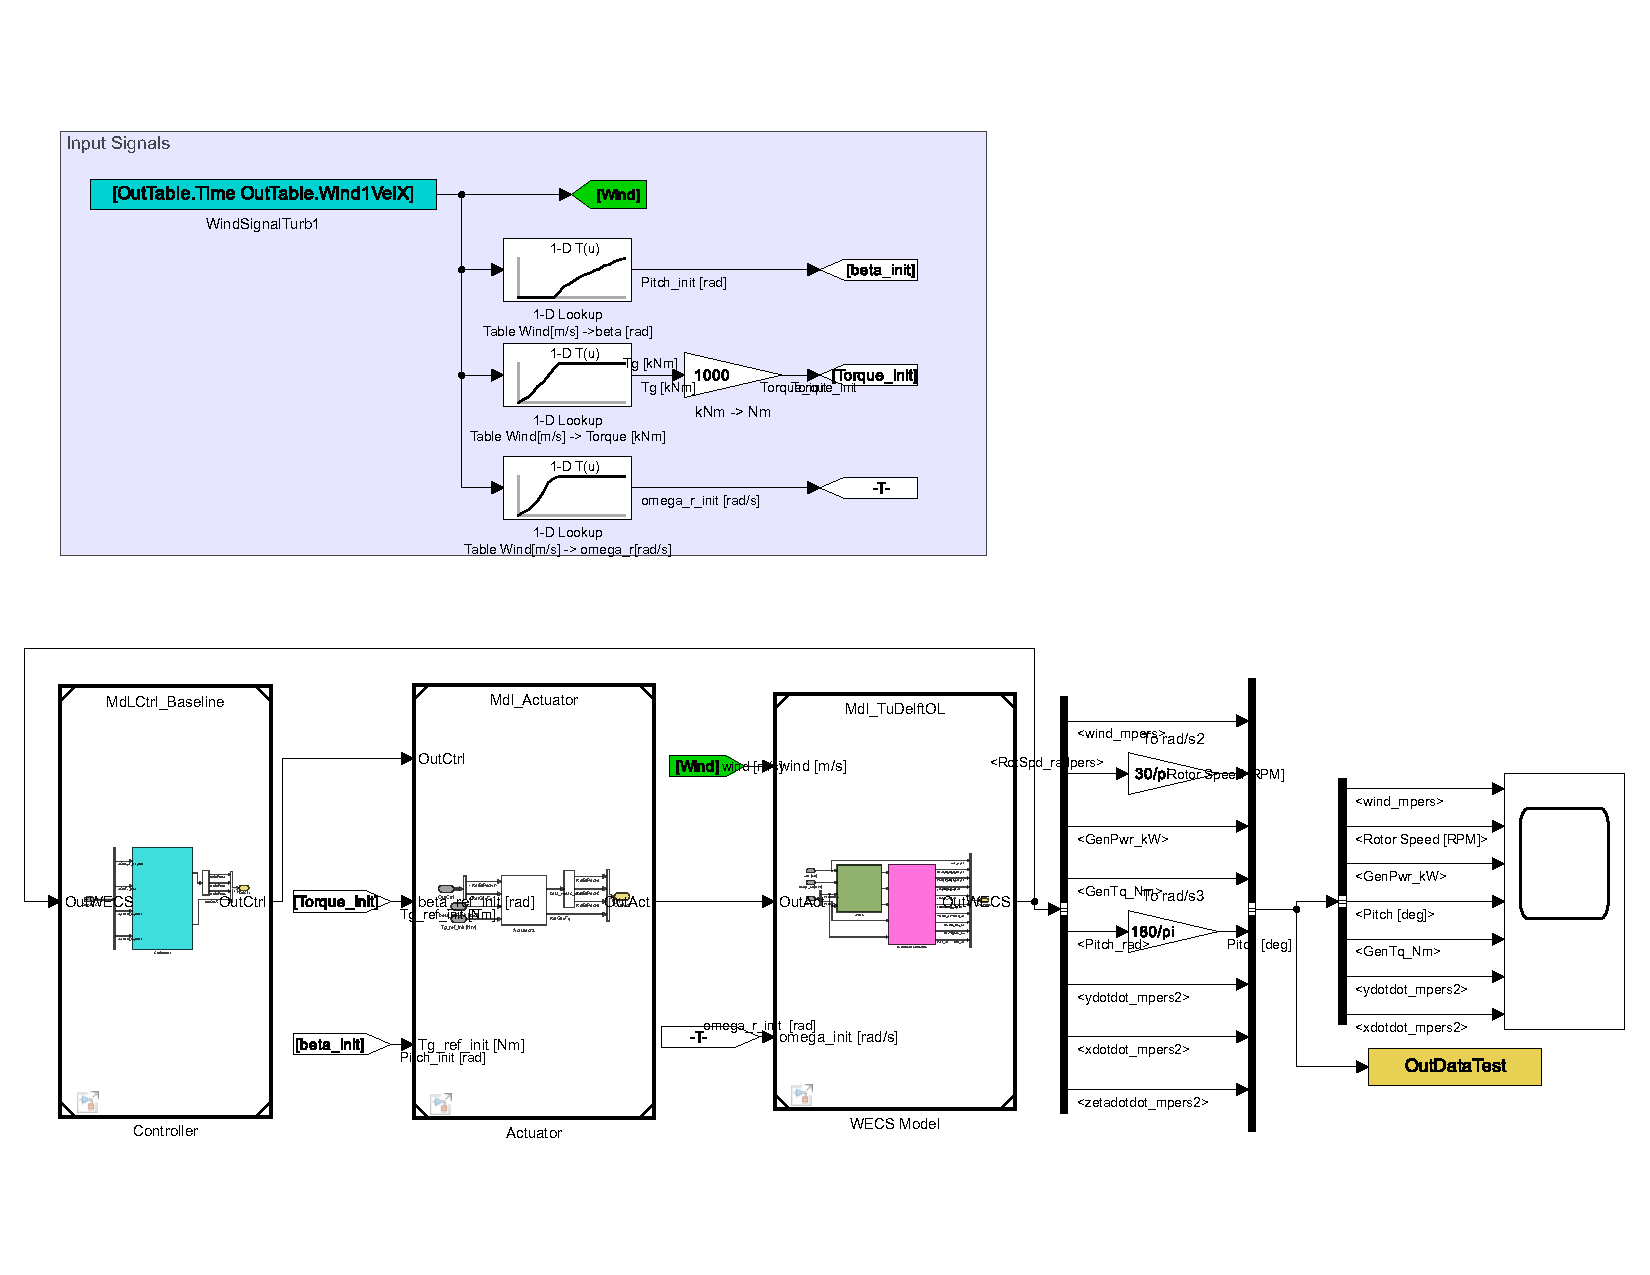
\includegraphics[width=0.9\textwidth, trim={0.2cm 2cm 0.2cm 2.cm}, clip]{figures/figures_Simulink/test_SimulinkMdl1_Baseline.pdf}
    \caption[Simulink model for closed loop verification including controller, actuator, and WECS model.]{Simulink model for closed loop verification including controller, actuator, and WECS model. The wind is created with the FASTTool and used for the initialization of the generator torque, the blade pitch and the rotor speed.}
   \label{fig:baseline_simulink}
\end{figure}
The baseline controller relies solely on generator speed feedback \(\omega_g\) and operates based on different control strategies across the turbine's operational regions. In Regions I 1/2 and II, the generator torque is determined using a \(k\omega^2\) control law, derived from a tabulated function of \(\omega_g\), maximizing power yield below rated wind speed. In Region III, a gain-scheduled PI controller modulates the collective blade pitch angle \(\beta_0\) to regulate power output. The proportional and integral gains, \(K_P(\omega_g)\) and \(K_I(\omega_g)\), are dynamically scheduled to track and maintain the rated rotor speed.
%
To prevent excitation of structural resonances, the FASTTool controller includes filters on the generator speed signal, such as a low-pass filter and two notch filters. The pitch control signal \(\beta_{\text{ref}}\) is determined based on the filtered generator speed \(\omega_{g,\text{filt}}\), ensuring stable power regulation above rated wind speed while mitigating structural loads. The controller allows for user selection between constant and gain-scheduled PI coefficients, with the latter used as the default setting, as detailed in \cite{mulders2020wind}.

The wind turbine model included in the Simulink implementation for closed loop testing is either the 5th or the 9th-order model described in Section~\ref{subsec:Structural Models}. Figure \ref{fig:ol_wecs_models} shows both models.
    
\begin{figure}[htbp]
    \centering
    \subfloat[5th-order model with rotor speed and tower displacement states, adapted from \cite{mulders2020preventing}.\label{fig:tudelft_ol_wecs}]{%
        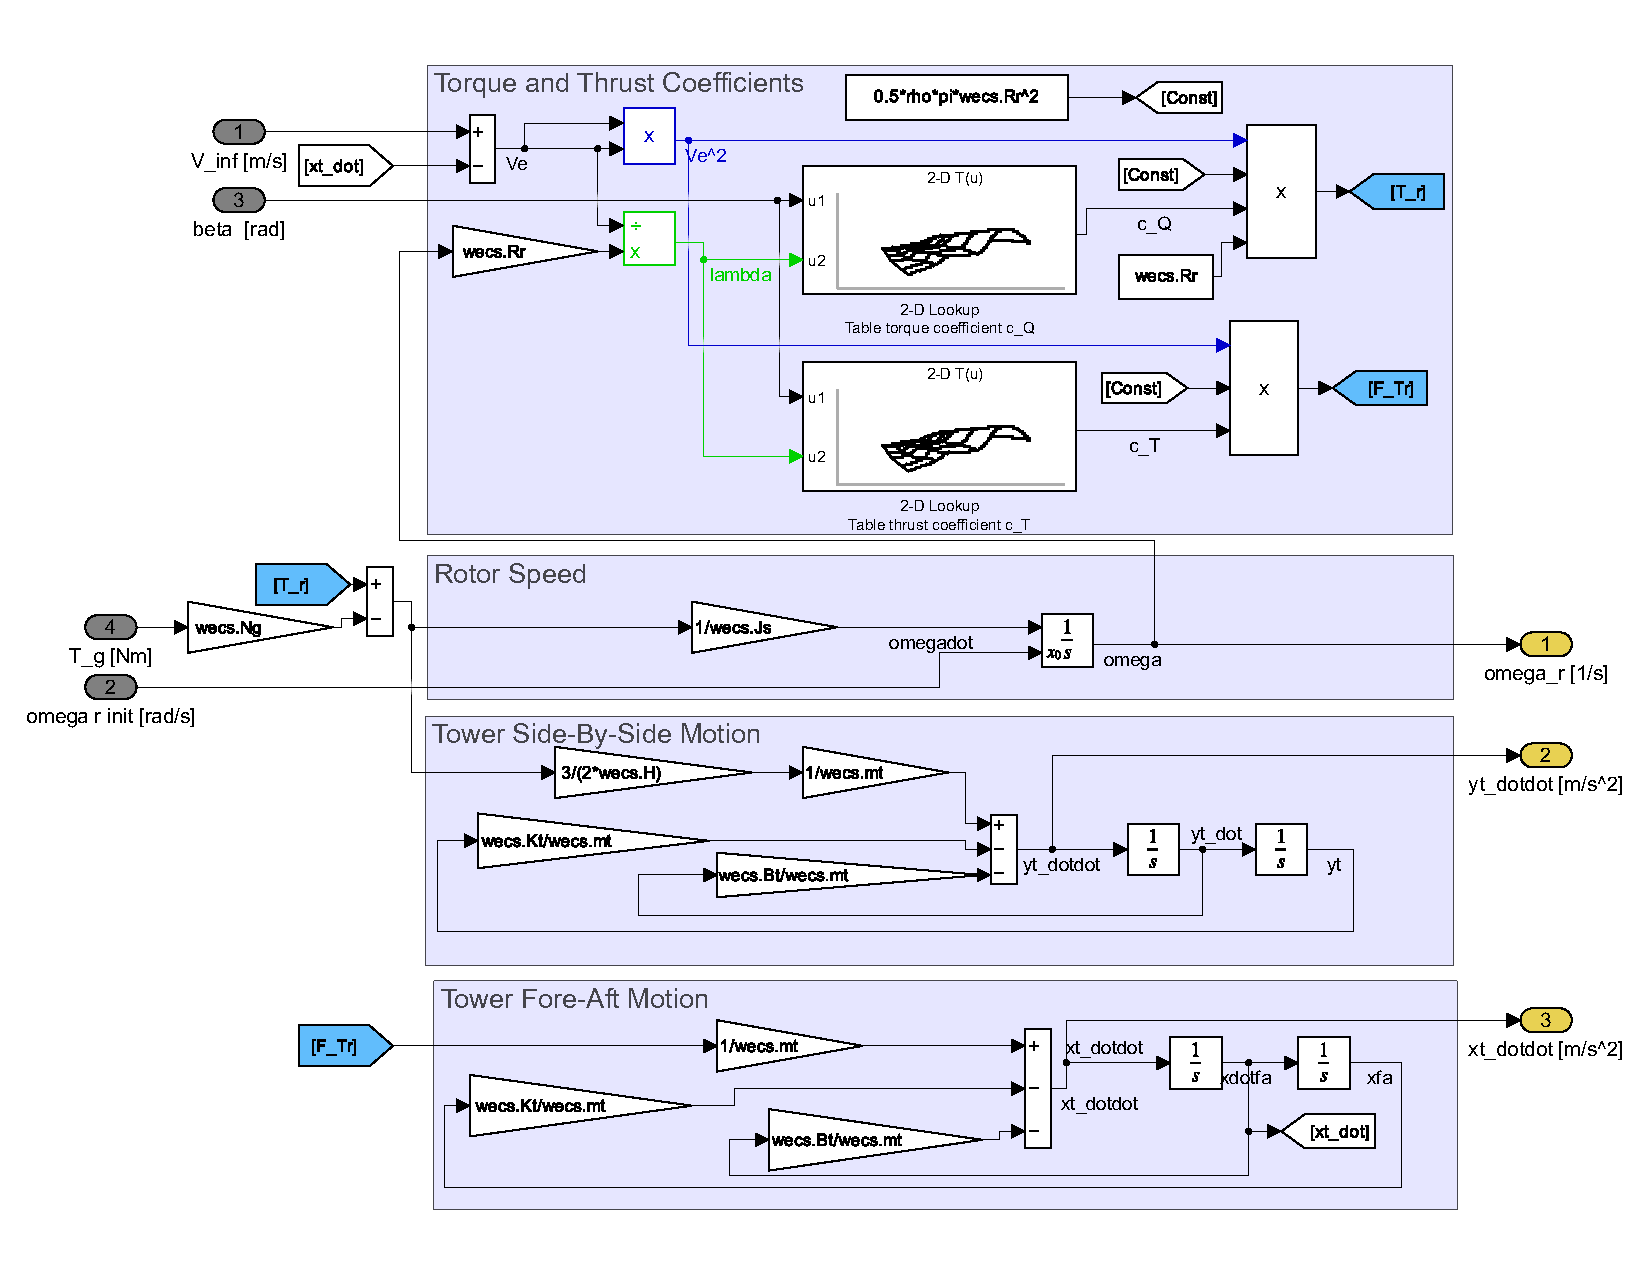
\includegraphics[width=0.9\textwidth, trim={0.2cm 0.5cm 0.2cm 1.cm}, clip]{figures/figures_Simulink/Mdl_TuDelftOL_WECS.pdf}
    }\\[1em]
    \subfloat[9th-order model with rotor and generator speed as well as tower and blade displacement states, adapted from \cite{Bianchi2007}.\label{fig:bianchi_ol_wecs}]{%
        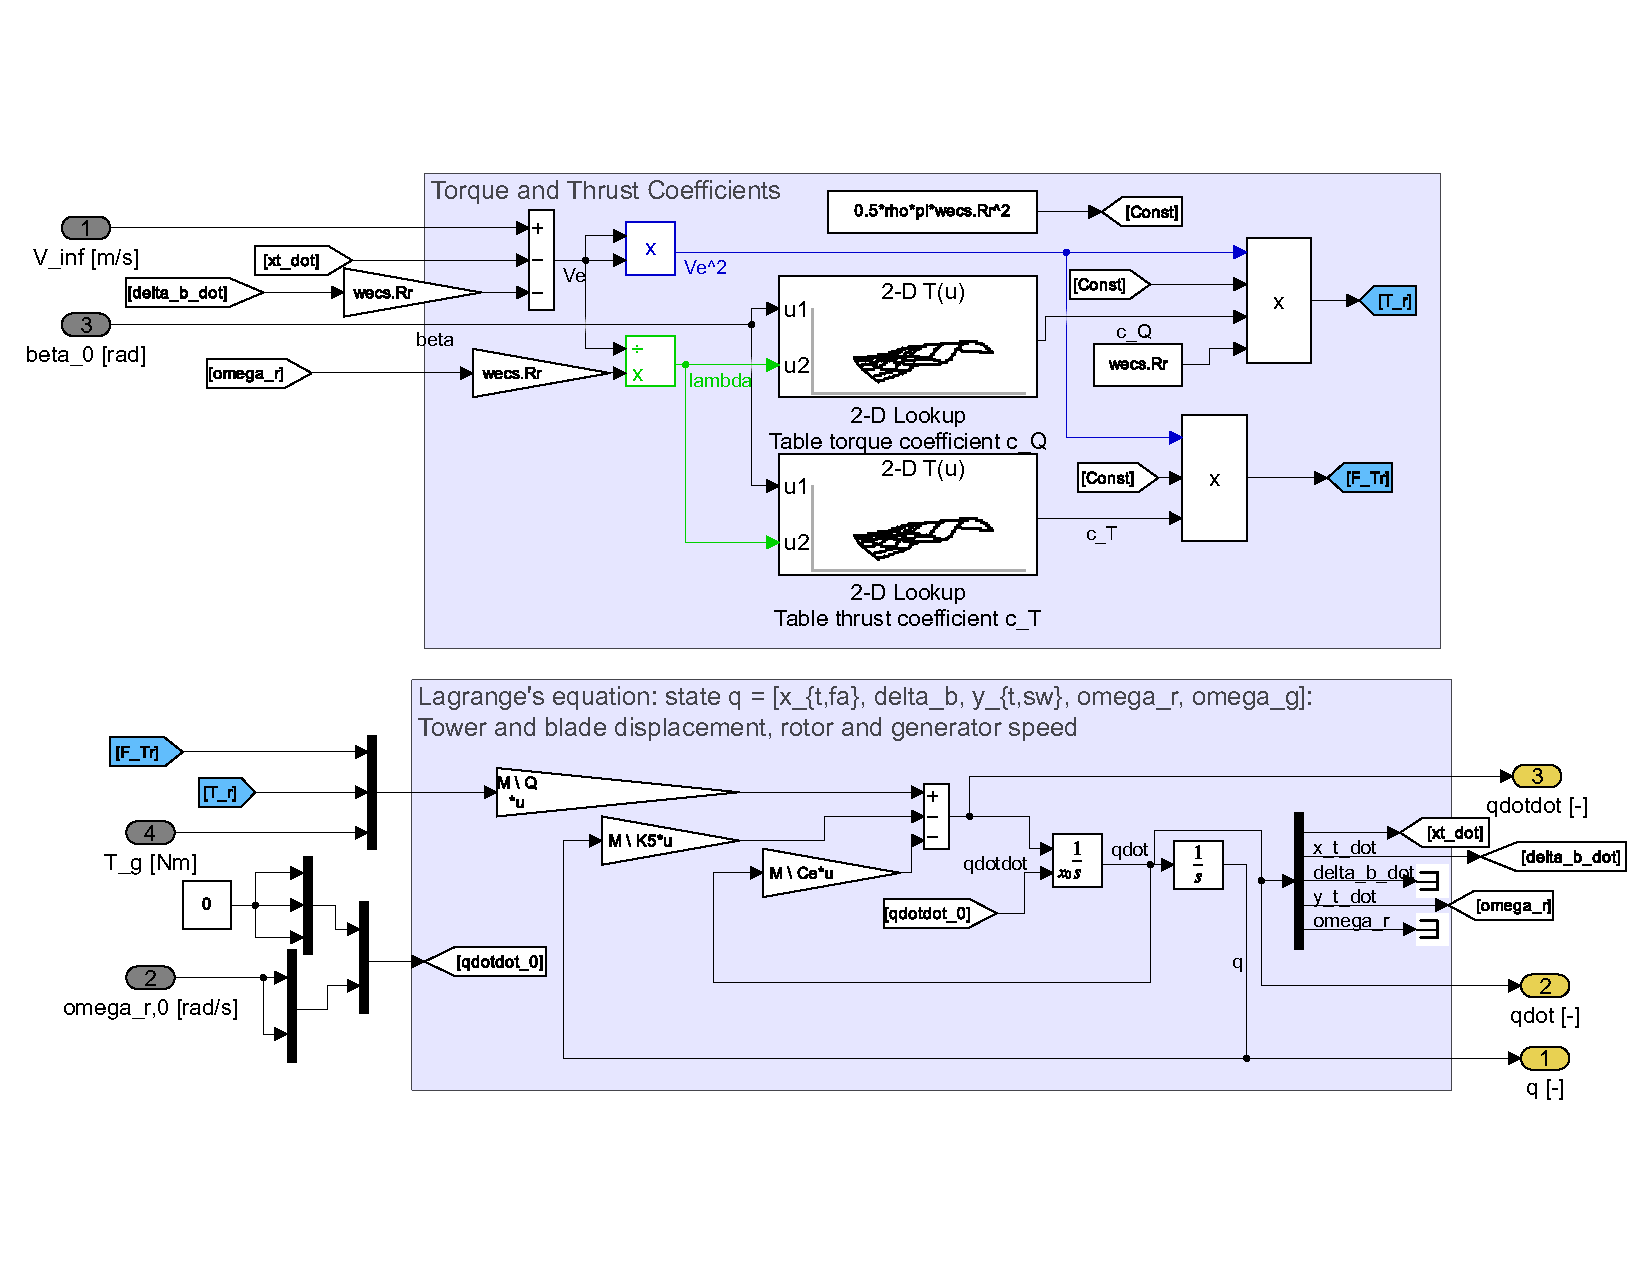
\includegraphics[width=0.9\textwidth, trim={0.1cm 2cm 0.2cm 2.8cm}, clip]{figures/figures_Simulink/Mdl_BianchiOL_WECS.pdf}
    }
    \caption[Simulink implementations of the two qLPV WECS models.]{Simulink implementations of the two qLPV WECS models. Both models use 2D lookup tables for the torque and thrust coefficient $c_T$ and $c_Q$, and have as inputs wind speed $V_\infty$, blade pitch angle $\beta$, and generator torque $T_g$.}
    \label{fig:ol_wecs_models}
\end{figure}

FASTTool is a MATLAB-based GUI used for configuring simulations and tuning controller parameters. It uses the FORTRAN-based FAST NREL 5MW wind turbine model implementation and integrates it into Simulink as an S-function. The baseline power controller is implemented using Simulink blocks and MATLAB functions. This controller is used to control both wind turbine models introduced above, as well as the Simulink S-function implementation of the FAST model. In the MIMO controller architecture presented in the next chapter, both the pitch and generator torque controllers of the baseline controller are replaced by the qLMPC scheme. For model verification purposes, however, the original Simulink implementation of the baseline controller is retained. The nonlinear differential equations of the two qLMPC models are implemented in Simulink. To verify the models, two simulations are performed using the original setup, including the baseline controller and the FAST NREL 5MW model implemented as an S-function. The first simulation consists of a wind-speed sweep from 4\,m/s to 25\,m/s in increments of 1\,m/s. Each wind-speed level is maintained for 100\,s to ensure that steady-state conditions are reached. This test is used to verify that the models converge to the same steady-state operating points and to compare their transient responses to wind-speed changes. The second simulation uses a turbulent wind field with a mean wind speed of 18\,m/s and IEC turbulence class B, corresponding to a turbulence intensity of 14\,\%. This simulation is used to investigate the qLPV models' responses to turbulent wind conditions. The first simulation is run for 2200\,s and the second for 660\,s. Both simulations are executed with a sampling time of 8\,ms, and the generated wind data are stored. Using these recorded wind speed time series, the simulations are repeated with the FAST NREL 5MW S-function replaced by the Simulink implementations of the qLPV models.

\newpage
\subsection{Results}\label{subsec:ResultsqLPVModel}
This section presents the open-loop frequency domain and closed-loop time domain verification of the two qLPV models.
\subsubsection*{Results Open-loop Frequency Domain Verification}
Figures~\ref{fig:Bode4} and~\ref{fig:Bode12} depict the magnitude response of four linear models: two models at the vertex wind speeds of 4\,m/s and 25\,m/s, and two models near the rated wind speed of 11.4\,m/s (specifically at 11\,m/s and 12\,m/s). Corresponding linearized FAST models serve as the reference.
\begin{figure} [htp]\center
 
    \subfloat[Wind speed $V_{\infty} = 4$\,m/s]{\includegraphics[width=0.75\textwidth]{Figures_ADi/BodeV4.eps}}\\
    \subfloat[Wind speed $V_{\infty} = 11$\,m/s]{\includegraphics[width=0.75\textwidth]{Figures_ADi/BodeV11.eps}}
   % \subfloat[Wind speed $V_{\infty} = 12$\,m/s]{\includegraphics[width=0.75\textwidth]{Figures_ADi/BodeV12.eps}}\\ 
  %  \subfloat[Wind speed $V_{\infty} = 25$\,m/s]{\includegraphics[width=0.75\textwidth]{Figures_ADi/BodeV25.eps}}
    \caption[Open-loop verification: Frequency response magnitude of linearized FAST and qLPV models for below rated wind speeds.]{Open-loop verification: Frequency response magnitude of linearized FAST and qLPV models for below rated wind speeds. Mdl1 (black dashed line), Mdl2 (blue line), and FAST reference implementation (red line) at frequencies from 0.01\,Hz to 2\,Hz.} %
    \label{fig:Bode4}
\end{figure}
\begin{figure} [htp]\center
    \subfloat[Wind speed $V_{\infty} = 12$\,m/s]{\includegraphics[width=0.75\textwidth]{Figures_ADi/BodeV12.eps}}\\ 
\subfloat[Wind speed $V_{\infty} = 25$\,m/s]{\includegraphics[width=0.75\textwidth]{Figures_ADi/BodeV25.eps}}
\caption[Open-loop verification: Frequency response magnitude of linearized FAST and qLPV models for above rated wind speeds.]{Open-loop verification: Frequency response magnitude of linearized FAST and qLPV models for above rated wind speeds. Mdl1 (black dashed line), Mdl2 (blue line), and FAST reference implementation (red line) at frequencies from 0.01\,Hz to 2\,Hz.} 
\label{fig:Bode12}
\end{figure}

 For all models, the frequency range from 0.01\,Hz to 2\,Hz is evaluated. Note that typically only the range up to 1\,Hz is considered in the literature, e.g., \cite{schlipf2013nonlinear} or \cite{pamososuryo2022individual}, as this interval contains the dominant first tower and blade modes. The magnitude response of the first (5th-order) model is shown in black, the second (9th-order) model in blue, and the linearized FAST reference in red. The latter's 30 states include all states of the derived qLPV models alongside additional structural degrees of freedom. The plots visualize the transfer functions from the control inputs (generator torque and blade pitch) and the disturbance (wind speed) to the rotor speed and tower fore-aft and side-to-side acceleration.
 
The comparison shows a good fit to the linearized FAST reference for both models from 0.01\,Hz up to the natural tower frequency at 0.3\,Hz. The second model also demonstrates a reasonable fit at the first blade natural frequency around 0.7\,Hz. However, the frequency behavior at higher frequencies exceeding 1\,Hz deviates from the FAST model. This deviation is due to higher-order dynamics present in the 30th-order linearized FAST model that are not captured in these simpler models. Thus, while the overall fit is reasonable, some discrepancy with the higher-order linearized FAST model is inevitable across different channels.

In the first column, the frequency response from the generator torque input is shown. From 0.01\,Hz up to approximately 0.7\,Hz, both reduced-order models follow the FAST reference closely. At lower wind speeds, depicted in Figure~\ref{fig:Bode4} as well as in Figure~\ref{fig:Bode12}(a), this is true for all three depicted output axes, i.e., the rotor speed, the tower fore-aft and side-to-side acceleration. At the highest wind speed, see Figure~\ref{fig:Bode12}(b), both models show a small deviation in the side-to-side acceleration at low frequencies that gradually closes as the tower frequency peak is approached. The side-to-side peak's frequency is captured accurately, though its magnitude is slightly underestimated. Above 1\,Hz, an additional resonance in the FAST reference, likely a blade mode, is not captured by either reduced-order model.

The second column shows the response to the blade pitch input. Blade pitch is not used for active control below rated wind speed, as in Figure~\ref{fig:Bode4}, and remains near a fixed angle. The pitch-to-output response therefore reflects the underlying open-loop aeroelastic dynamics, in which blade structural modes play a dominant role. As a result, differences between the reduced-order models become more apparent in this channel. Looking at the response of the rotor speed to the blade pitch, the agreement between the FAST reference and the 9th-order model is considerably better than with the 5th-order model. The advantage of the model with blade dynamics is also clear in the tower fore-aft acceleration response, where it reproduces the blade frequency peak around 0.7\,Hz, especially at 4\,m/s in Figure~\ref{fig:Bode4}a. At higher wind speeds, see Figure~\ref{fig:Bode12}, this peak is less pronounced, and differences among models diminish. Still, the 9th-order model, which includes blade dynamics, consistently provides a better overall fit across the full frequency range for the responses of the rotor speed and tower fore-aft acceleration. Interestingly, in the tower side-to-side acceleration response, the model without blade dynamics outperforms the one including them, particularly at low frequencies. This is likely because the blade mode in the 9th-order model is tuned to match fore-aft motion, which dominates the tower bending, whereas side-to-side effects require more detailed blade modeling than currently included.

The third column depicts the response to variations in wind speed. In the rotor speed response, a sharp notch appears in the FAST reference at approximately 0.34\,Hz, the frequency of the first tower mode, across all wind speeds. Both qLPV models reproduce this notch closely. At higher frequencies, however, Mdl1 continues along a smooth, monotonic decline, while Mdl2 dips more sharply at 0.7\,Hz before recovering to follow the slope of Mdl1. FAST does not dip at 0.7\,Hz, but at 0.8\,Hz for the two lower and around 1\,Hz for the higher wind speeds, still the amplitude of Mdl2 is closer to this reference than the one of Mdl1.

In the tower fore-aft acceleration response, both models again match FAST well through the tower peak at 0.34\,Hz. Past the peak, Mdl2 continues to track the FAST reference's mild increase at 0.7\,Hz, whereas Mdl1 diverges gradually as its response flattens. In both of these channels, Mdl2 therefore clearly outperforms Mdl1 at higher frequencies. In the tower side-to-side response, by contrast, Mdl1 and Mdl2 remain close to one another throughout the frequency range, but both substantially overestimate the FAST reference at low frequencies, with the gap closing as all three converge near the shared tower peak at 0.34\,Hz. Above this peak, the FAST reference drops, with this amplitude decrease not reproduced by either qLPV model. Instead, Mdl2 exhibit a secondary dip near 0.7\,Hz that is largely absent from the FAST reference, while Mdl1 shows a relative flat response. However, despite the comparatively weaker open-loop fit in the side-to-side channel, it will be discussed in the next section that this discrepancy has little practical impact. To verify that the reduced-order models accurately capture the dynamics within the frequency range relevant for control, a time-domain comparison with the FAST reference is also carried out in closed-loop operation. 


\subsubsection*{Results Closed-loop Time Domain Verification}    
For the verification in closed loop, two representative wind scenarios are considered: a stepped wind speed sweep from 4\,m/s to 25\,m/s, and a turbulent wind input with a mean speed of 18\,m/s.

Figure~\ref{fig:TimeCmpMdlSweep}(a) shows the results for the stepped wind sweep across all three closed-loop models. The wind increases in steps of 1\,m/s every 100\,s. The first 60\,s of the simulation, which contain initialization artifacts, are omitted. As a result, 40\,s of excitation is shown for 4\,m/s, and 100\,s for all other wind speeds. Figure~\ref{fig:TimeCmpMdlSweep}(b) presents the signals between 600\,s and 1000\,s of simulation time, corresponding to wind speeds between 10\,m/s and 13\,m/s. As before, the signals of the 5th-order model are plotted in black (dashed), the 9th-order model in blue, and the FAST model in red.
\begin{figure}[h]
    \centering
    \subfloat[Stepped wind sweep from 4\,m/s to 25\,m/s]{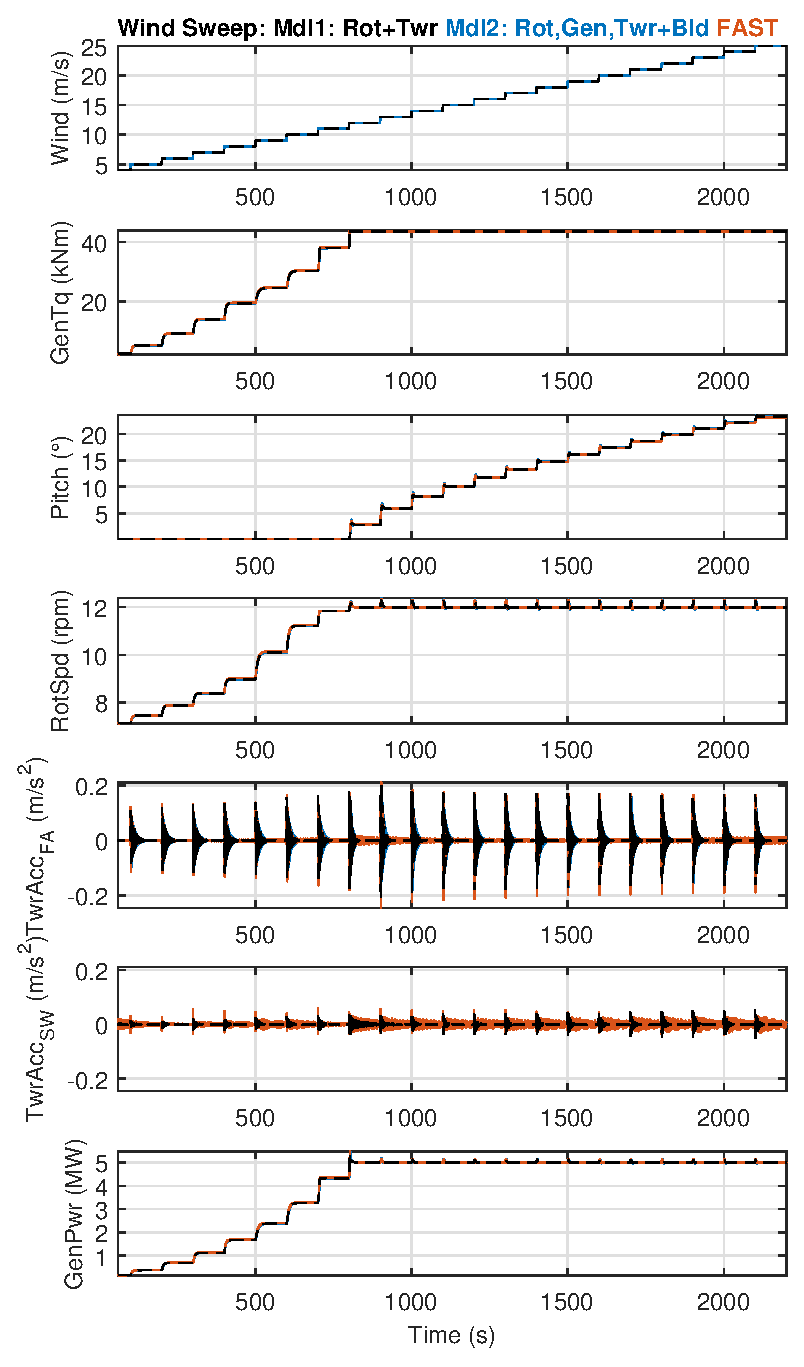
\includegraphics[width=0.435\textwidth]{figures/Figures_ADi/cmpTimeDomain_All.eps}}\hspace{0.01\textwidth}
    \subfloat[Zoom on wind speed range 10\,m/s to 13\,m/s]{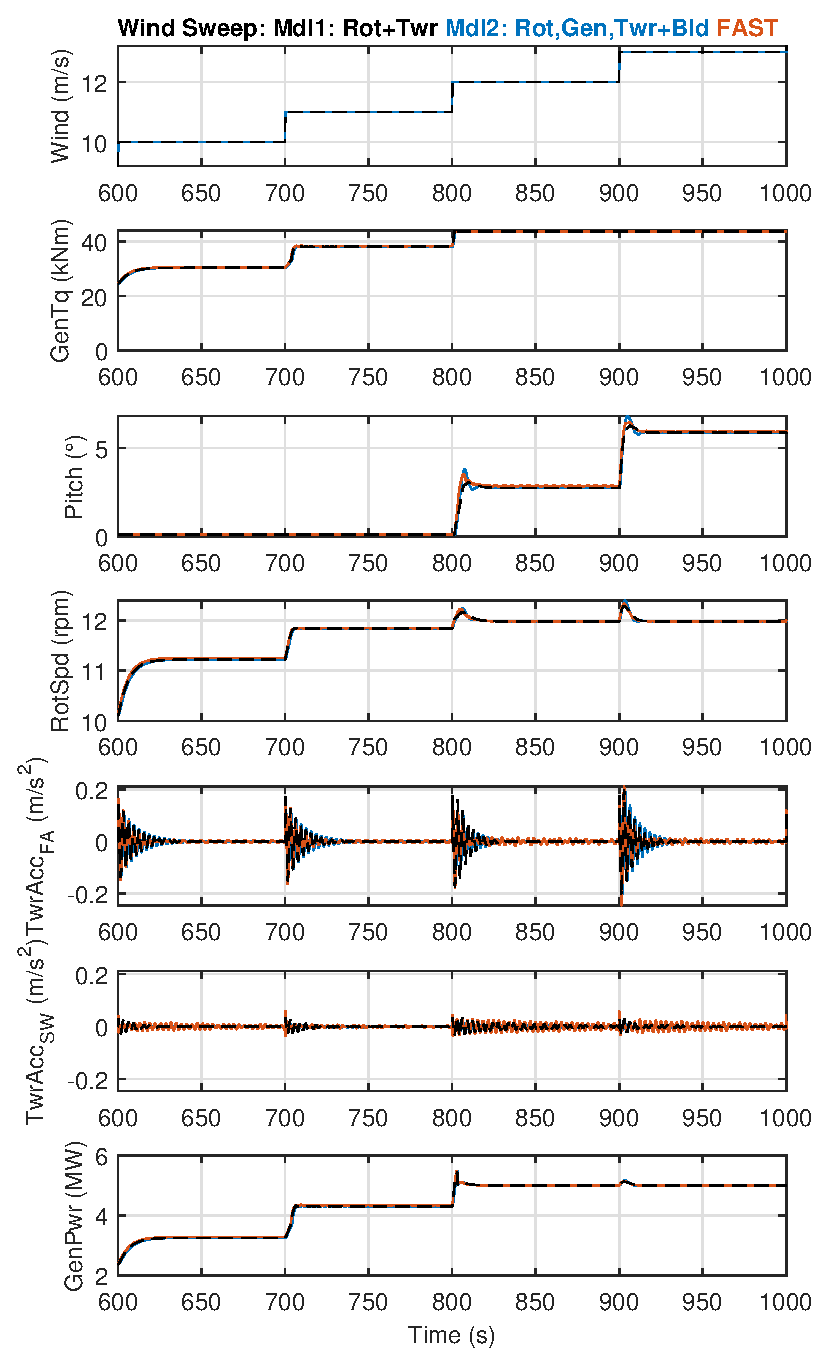
\includegraphics[width=0.45\textwidth]{figures/Figures_ADi/cmpTimeDomain_AllZoom.eps}}
    \caption[Closed-loop verification: FAST and qLPV models with PI baseline 
   controller, stepped wind sweep 4\,m/s to 25\,m/s.]%
   {Closed-loop verification: FAST and qLPV models simulated in closed loop with the PI baseline controller with a stepped wind sweep from 4\,m/s to 25\,m/s. 
       Mdl1 (black dashed line), Mdl2 (blue line), and FAST reference implementation (red line). Displayed signals: wind, control inputs, 
       rotor speed, tower accelerations, and power.}
    \label{fig:TimeCmpMdlSweep}
\end{figure}
%
The first subplot shows the wind input applied to the turbine, which is identical for all simulations. The second and third subplots display the two control inputs: generator torque and collective blade pitch. The fourth subplot shows the rotor speed, followed by the fifth and sixth subplots showing the tower fore-aft and side-to-side accelerations, respectively. The final subplot depicts the resulting electrical power output. There is an excellent fit between FAST and both models for the stepped wind sweep test case, in the transient dynamic as well as in the steady state gain. The good fit in steady state corresponds to the resemblance between FAST and both models for the rotor speed and the tower fore-aft acceleration for lower frequencies. As there is little difference both in the generator torque as well as in the rotor speed, there is also a good fit in the power output. There is also a good fit in the amplitude of the fore-aft tower acceleration for all wind speeds. The only signal that is not matched well is the tower side-to-side acceleration. However, the amplitudes of this signal is comparably small and its influence on the overall dynamics is nearly negligible.

Figure~\ref{fig:TimeCmpMdlNTM} shows the second test case: a turbulent wind profile with a mean speed of 18\,m/s and IEC turbulence class B. This test case reveals a limitation of the qLPV models, which represent wind as a scalar value acting uniformly on the rotor, rather than as a spatially distributed field.
\begin{figure}[h]
    \centering
    \subfloat[No filter]{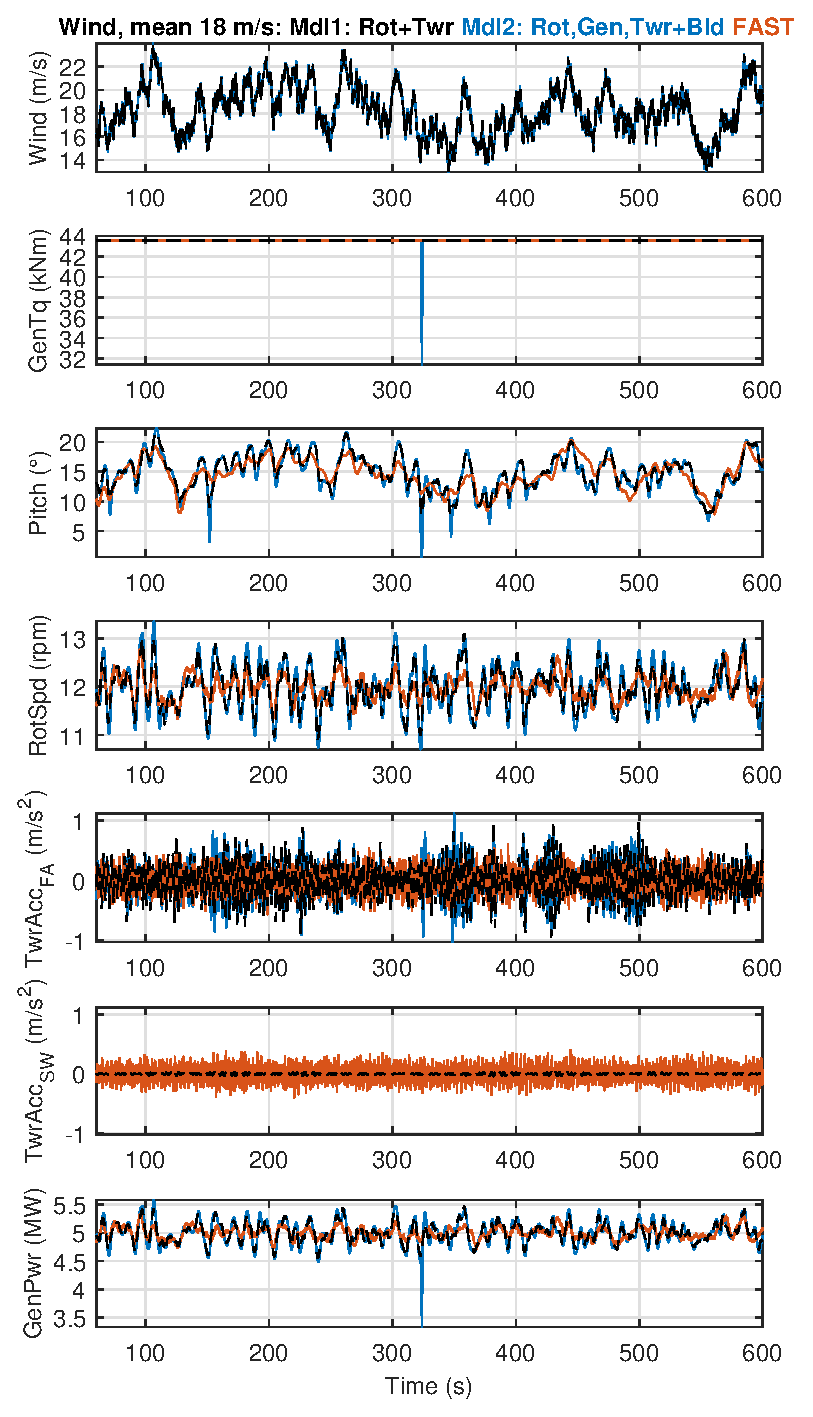
\includegraphics[width=0.45\textwidth]{figures/Figures_ADi/cmpTimeDomain_AllNTW18.eps}}\hspace{0.01\textwidth}
    \subfloat[Filter with $k_\tau = 0.75$ and  $k_T = 0.25$ ]{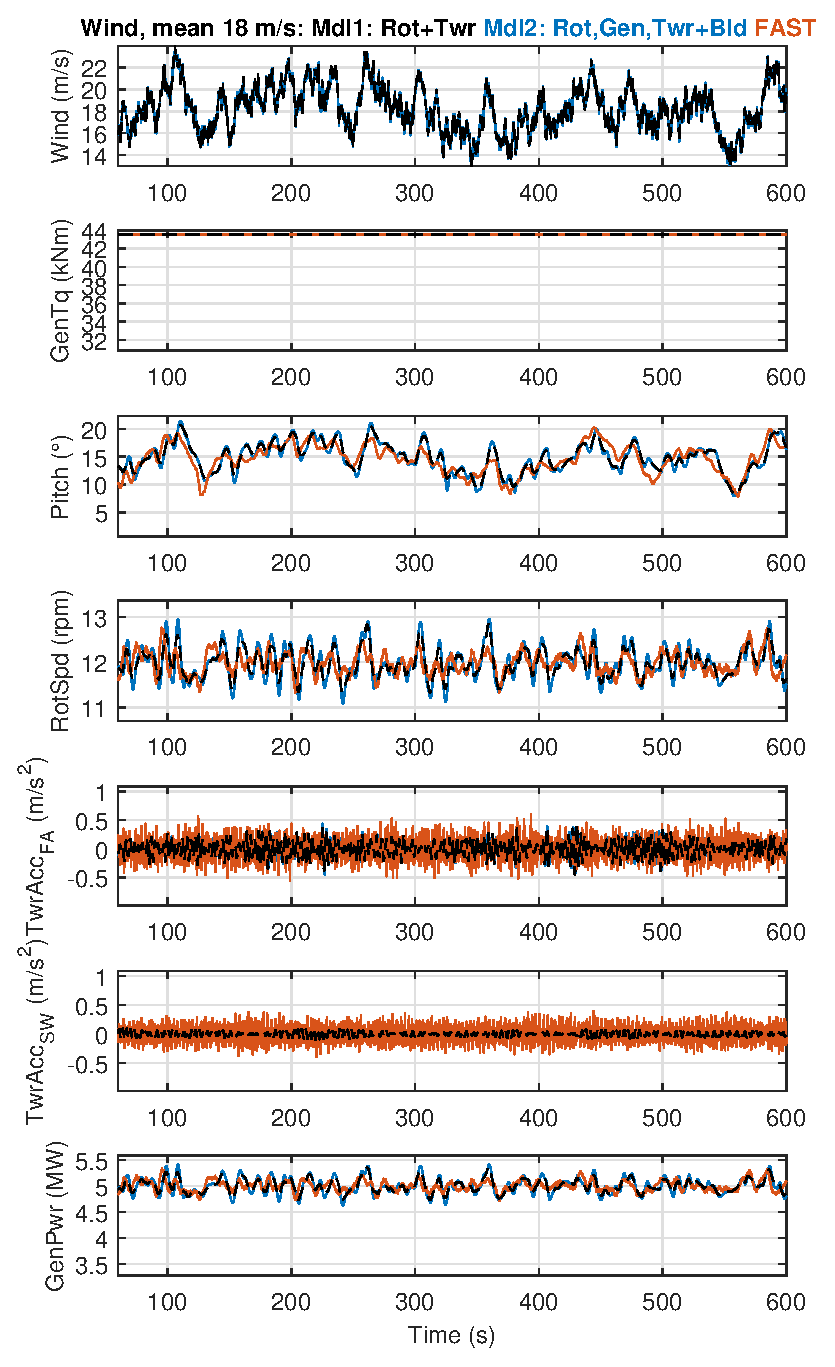
\includegraphics[width=0.45\textwidth]{figures/Figures_ADi/cmpTimeDomain_AllNTW18_kVe0dot25_kVeTau0dot75.eps}}
    \caption[Closed-loop model comparison: FAST and qLPV models with baseline 
    PI controller, under turbulent wind with and without filter on freestream wind.]{Closed-loop model comparison: FAST and qLPV models with PI baseline controller, under turbulent wind, 18\,m/s mean, IEC turbulence 
        class B (14\,\%), with and without filter on freestream wind. Mdl1 (black 
        dashed line), Mdl2 (blue line), and FAST reference implementation (red 
        line). Displayed signals: wind, control inputs, rotor speed, tower 
        accelerations, and power.}
    \label{fig:TimeCmpMdlNTM}
\end{figure}
In a real turbine, the large rotor disk acts as a natural low-pass spatial 
filter, averaging out high-frequency point gusts across its swept area. 
Because single-point freestream wind files lack this spatial coherence, 
feeding an unfiltered point velocity into the low-order lookup tables causes 
the model to respond excessively to high-frequency variations. At the same 
time, structural tower dynamics are driven by localized aerodynamic thrust 
forces and blade-passage effects, which require a faster excitation spectrum. 
To address this discrepancy, a velocity-dependent low-pass filter is applied 
to the freestream wind input, with separate scaling factors for the torque 
($k_\tau = 0.75$) and thrust ($k_T = 0.25$) channels to preserve the 
relevant excitation frequencies for each. As shown in Figure~\ref{fig:TimeCmpMdlNTM}(a), without filtering the models 
exhibit pronounced high-frequency oscillations and overshoot in blade pitch, 
rotor speed, and generator power. With the filter active in Figure~\ref{fig:TimeCmpMdlNTM}(b), the amplitudes more 
closely follow the FAST reference while the tower fore-aft acceleration 
retains sufficient high-frequency excitation. Note that these filters are used 
only for the turbulent wind comparison with FAST and are not included in the 
qLMPC controller design, where the freestream wind speed $V_\infty$ is used 
directly as an input.

It should also be noted that some minor discrepancies remain in Figure~\ref{fig:TimeCmpMdlSweep}, such as small oscillations in the tower movement due to FAST's full degrees of freedom. However, the reduced-order models capture the dominant system dynamics with sufficient accuracy for control design. Both Mdl1, without blade dynamics, and Mdl2, with an additional blade flapwise degree of freedom, show good agreement with the FAST reference during the stepped wind sweep. Mdl2 captures a broader range of dynamics, most notably in the blade pitch to rotor speed channel, where it shows better alignment with FAST due to the inclusion of blade dynamics. Furthermore, Mdl2 enables the representation of blade out-of-plane moments, which is relevant for evaluating damage equivalent loads used as one of the performance criteria for controller evaluation. Therefore, Mdl2 is selected as the basis for the qLMPC design.


    \chapter{Wind Turbine Control}  \label{sec:Application to Wind Turbine Control4}

%Modern megawatt wind turbines are both speed-controlled and pitch-controlled \cite{pao2011control, mulders2018delft, elkodama2023control}. Controllers and their parameters are often fine-tuned to fit not only a specific wind turbine type but also individual turbines, taking into account factors such as manufacturing and installation variations, including rotor blade weight imbalances and aging processes \cite{en14238083}. These conventional feedback control designs, typically relying solely on generator speed as input and controlling the blade pitch angles collectively, are well-engineered and technologically mature. However, further reduction of the cost of energy production can be achieved by introducing additional control inputs or sensors. Moreover, using a predictive scheme like qLMPC allows leveraging wind measurements or estimates and incorporating this information over a prediction horizon. It also accounts for how the system states, e.g., the rotor and generator speed, are expected to react to the wind trajectory and future control inputs within that horizon. This chapter investigates control strategies that leverage such improvements: a qLMPC design, which incorporates preview wind information, and PI Individual Pitch Control (IPC), the latter both as a standalone method and in combination with Trailing Edge Flap Control (TEFC), aimed at reducing mechanical loads. These control approaches are evaluated in terms of power reference tracking, actuator activity, and mechanical loads.
%In Section~\ref{sec:quasiLPVMPCDesign}, the design of a velocity-based qLMPC controller based on a first-principles model is presented. Section~\ref{section:Individal Pitch PI Control} introduces IPC, explaining the multi-blade coordinate transformation and comparing IPC simulation results to those from baseline Collective Pitch Control (CPC). Section~\ref{sec:CombinedIPC-TrailingEdgeFlapControl} describes the combination of IPC and TEFC, including the necessary model extensions and the achieved load reductions on the blades and tower. A brief comparison and conclusion section summarizes the results obtained with the three wind turbine controller designs. The results for the qLMPC controller have been published in \cite{dittmer2021velocity}, and the TEFC control strategy in \cite{dittmer2024combined}.
%  
Modern megawatt wind turbines are both speed-controlled and pitch-controlled \cite{pao2011control,
    mulders2018delft, elkodama2023control}. Controllers and their parameters are often fine-tuned to
fit not only a specific wind turbine type but also individual turbines, taking into account factors
such as manufacturing and installation variations, including rotor blade weight imbalances and
aging processes \cite{en14238083}. These conventional feedback control designs, typically relying
solely on generator speed as input and controlling the blade pitch angles collectively, are
well-engineered and technologically mature. However, further reduction of the cost of energy
production can be achieved by introducing additional control inputs or sensors. Moreover, using a
predictive scheme like qLMPC allows leveraging wind measurements or estimates and incorporating
this information over a prediction horizon. It also accounts for how the system states, e.g., the
rotor and generator speed, are expected to react to the wind trajectory and future control inputs
within that horizon. This chapter investigates control strategies that leverage such improvements:
a qLMPC design, which incorporates preview wind information, and PI Individual Pitch Control
(IPC), the latter both as a standalone method and in combination with Trailing Edge Flap Control
(TEFC), aimed at reducing mechanical loads. These control approaches are evaluated in terms of
power reference tracking, actuator activity, and mechanical loads.

In Section~\ref{sec:quasiLPVMPCDesign}, the design of a velocity-based qLMPC controller based on
the first-principles model of Chapter~\ref{sec:WindTurbineqLPVModels} is presented. Where qLMPC
has so far been applied to wind turbines as a SISO scheme \cite{mulders2020preventing, pamososuryo2022individual,
    fonseca2024windTurbineSideSide}, the design presented here actuates generator torque and
collective pitch simultaneously as a MIMO scheme, covering the entire operating range. It is
reformulated as a QP and solved via a linear complementarity formulation with Lemke's algorithm
\cite{cisneros2020velocity}, yielding mean solver times below 2\,ms at a controller sampling time
of 8\,ms and thus real-time capability.
%
Section~\ref{section:Individal Pitch PI Control} introduces IPC, explaining the multi-blade
coordinate transformation and comparing IPC simulation results to those from baseline Collective
Pitch Control (CPC). The simulation environment is also used to tune the IPC gains, by a grid
search followed by a Nelder-Mead simplex optimization of the blade root DEL.
%
Section~\ref{sec:CombinedIPC-TrailingEdgeFlapControl} describes the combination of IPC and TEFC,
including the necessary model extensions and the achieved load reductions on the blades and tower.
Whereas earlier studies combining the two actuation principles report results for single mean wind
speeds \cite{wilson2009combined, henriksen2013model, he2018combined}, the controller presented
here is demonstrated across Regions II and III, using one training data set and two independent
verification data sets. A final comparison section evaluates qLMPC, IPC, and AALC against each
other, showing the trade-off between DEL reduction and actuator activity relative to the PI CPC
baseline. The results for the qLMPC controller have been published in \cite{dittmer2021velocity},
and the TEFC control strategy in \cite{dittmer2024combined}.
\section{qLMPC Design and Application}\label{sec:quasiLPVMPCDesign}
Wind turbine controller design in above rated region focuses on smooth power control and in the below rated region on power optimization, as described in \cite{Bianchi2007}. Generator speed reference tracking is achieved using two control inputs: the collective blade pitch angle $\beta_{0,\text{ref}}$ and the generator torque reference $T_{g,\text{ref}}$. The baseline controller consists of two SISO controllers, one for generator torque and one for blade pitch control, see Section~\ref{sec:WindTurbineControl}. These can be replaced by a MIMO qLMPC power controller, see Figure \ref{fig:BlockMPC}. The qLMPC is designed to track rotor and generator speed references while minimizing changes in the control inputs, resulting in smoother power output and reduced tower movement compared to the baseline. DEL reduction is not an explicit objective of the qLMPC design. However, the five evaluation criteria used to compare all control strategies introduced in Section~\ref{subsection Control Objectives}, i.e., blade and tower DEL, power mean and variance, and actuator activity, are also calculated for this controller to enable a direct comparison with the IPC and AALC designs.

\begin{figure}[ht]
    \centering
    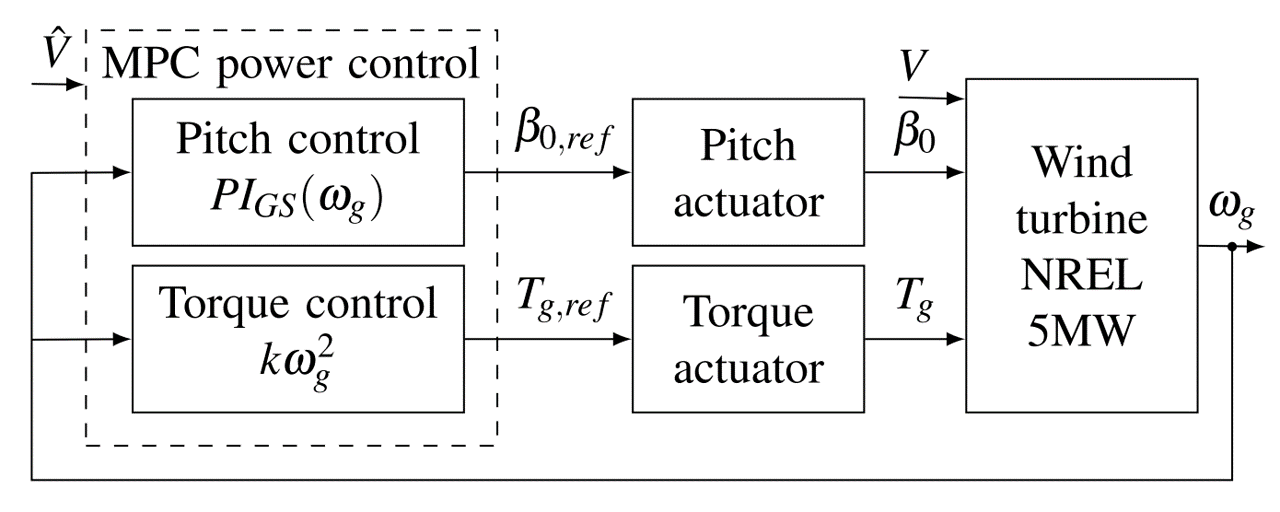
\includegraphics[width=0.8\textwidth,trim={0 0cm 0cm 0.3cm},clip]{figures/Figures_ADi/turbineMPC.png}
    \caption[Block diagram of the closed-loop wind turbine control structure with qLMPC replacing the baseline PI controller]{Block diagram of the closed-loop wind turbine control structure with qLMPC (dashed box) replacing the baseline PI controller (solid line)}
    \label{fig:BlockMPC}
\end{figure}

In this work, the velocity based approach from \cite{cisneros2020velocity}, presented in section \ref{windTurbineModel} of this thesis, is applied: A $3^{rd}$ order wind turbine model, used as the basis for quasiLPV based MIMO controller design in \cite{Bianchi2007}, is implemented with some minor changes. To model the main dynamics, it is sufficient to consider the slip angle $\theta_s$, the rotor and generator speed $\omega_r$ and $\omega_g$. The same states are considered here, but three modifications were made:
\begin{enumerate}
    \item A filtered generator torque $T_g^{\prime} = T_{g,\text{ref}}$ is introduced as an additional state to eliminate direct throughput, i.e., to avoid a non-zero feedthrough matrix \( \bm{D} \). This fourth state enables the use of the optimization framework for reference tracking and disturbance rejection proposed in \cite{cisneros2020velocity}. Incorporating a filtered control input as an additional state is a common practice, and is, for example, also employed in the MPC algorithm implemented in WFSim \cite{boersma2018control}.    
    \item Reference generator torque $T_{g,\text{ref}}$ is used as a control output signal and plant input signal. In \cite{Bianchi2007}, the second control input is the zero torque speed $\omega_Z$ which is linearly dependent on the generator torque $T_{g}$. The reference torque is selected as it is the format of expected input signal to the wind turbine in the FAST implementation. The optimal trajectory of the reference generator torque  $T_{g,\text{ref}}$ over a prediction horizon is calculated based on an optimal reference signal $r_{\beta}$ which is itself calculated from the wind speed.
    \item A desired pitch signal $r_{\beta}$ is used as a reference for the prediction horizon in the MPC optimization to calculate the optimal controller output pitch signal $\beta_{0,\text{ref}}$. In \cite{Bianchi2007}, a reference value for the generator speed is tracked. This choice was made to directly optimize the two actuators to avoid handling the large difference in dynamic bandwidth of the actuators and the plant dynamics in the optimization calculation. Identical to the filtered generator torque, a filtered pitch $\beta_0^{\prime} = \beta_{0,\text{ref}}$ is introduced as a fifth state.
\end{enumerate}
%
The resulting states, input and output vectors are given below. As before, different indices are used for the generator speed in the high-speed shaft, denoted $\omega_g$, and the low-speed shaft, $\omega_{gr}$. In the state vector, the generator speed in the low-speed shaft is used as it operates in the same reference system as the rotor speed $\omega_r$:
\begin{align}\label{eq:xMPCyMPC}
    \bm{x}_{\text{MPC}} =[\theta_{s}  \quad {\omega}_r \quad {\omega}_{gr} \quad T_g^{\prime} \quad \beta_0^{\prime} ]^T  \in \mathbb{R}^{5 \times 1},   \quad \bm{y}_{\text{MPC}} = [T_{g,\text{ref}} \quad  {\beta}_{0,\text{ref}}]^T  \in \mathbb{R}^{2 \times 1}.
\end{align}
%
The nonlinear dynamics describing changes in the three turbine states are:
\begin{align}
    \dot{\theta_s}(t)&={\omega}_r(t)-{\omega}_{gr}(t) \label{eq:NLDyn1}\\
    \dot{\omega}_r(t)&=-\frac{K_{sr}}{J_r}\theta_s(t)-\frac{B_{sr}}{J_r}{\omega}_r(t)+\frac{B_{sr}}{J_r}{\omega}_{gr}(t)+\frac{T_r({\omega}_r, \beta, v)}{J_r}\\
    \dot{\omega}_{gr}(t)&=\frac{K_{sr}}{J_{gr}}\theta_s(t)+\frac{B_{sr}}{J_{gr}}{\omega}_r(t)-\frac{B_{sr}}{J_{gr}}{\omega}_{gr}(t)-\frac{N_gT_g(t)}{J_{gr}} \label{eq:NLDyn3} \\
 %   \dot{ T}^{\prime}_{g} &= -\frac{1}{ \kappa}T_{g} +\frac{1}{ \kappa}T_{g, ref}\\
%    \dot{\beta}^{\prime}_& = -\frac{1}{ \tau}\beta^{\prime} +\frac{1}{ \tau}\beta_{g, ref}
\end{align}
%
To avoid having to derive a grid of initial states for the different combinations of the state vector, a velocity based linearization is designed.
\subsection{Velocity-Based qLPV Model Linearization}
The velocity-based linearization method from \cite{cisneros2020velocity} is implemented for the model serving as the basis of the qLMPC design. The nonlinear system dynamics
\[
\dot{\bm{x}}_{\text{MPC}}(t) = \bm{f}_{\text{MPC}}(\bm{x}_{\text{MPC}}, \bm{w}_{\text{Mdl}}), \quad \bm{y}_{\text{MPC}}(t) = \bm{h}_{\text{MPC}}(\bm{x}_{\text{MPC}})
\]
are described by the relationship between the state and input derivatives: 
\begin{align*}
    \ddot{\bm{x}}_{\text{MPC}}(t) &= \nabla_{\bm{x}_{\text{MPC}}} \bm{f}_{\text{MPC}}(\bm{x}_{\text{MPC}}, \bm{w}_{\text{Mdl}}) \dot{\bm{x}}_{\text{MPC}}(t) + \nabla_{\bm{w}_{\text{Mdl}}}\bm{f}_{\text{MPC}}(\bm{x}_{\text{MPC}}, \bm{w}_{\text{Mdl}}) \dot{\bm{w}}_{\text{Mdl}}(t),\\
    \dot{\bm{y}}_{\text{MPC}}(t) &= \nabla_{\bm{x}_{\text{MPC}}}\bm{h}_{\text{MPC}}(\bm{x}_{\text{MPC}}) \dot{\bm{x}}_{\text{MPC}}(t).   
\end{align*}
By considering the derivatives instead of the original states, the need for storing steady-state vectors for input, output, and states at each operating point is omitted.
%

The continuous-time system, input, and output matrices,
\begin{align*}
      \bm{A}_c(\bm{\rho}_{\Rho}) &= \nabla_{\bm{x}_{\text{MPC}}} \bm{f}(\bm{x}_{\text{MPC}}, \bm{w}_{\text{Mdl}}),\\ 
      \bm{B}_c(\bm{\rho}_{\Rho}) &= \nabla_{\bm{w}_{\text{Mdl}}} \bm{f}(\bm{x}_{\text{MPC}}, \bm{w}_{\text{Mdl}}),\\ 
      \bm{C}_c(\bm{\rho}_{\Rho}) &= \nabla_{\bm{x}_{\text{MPC}}} \bm{h}(\bm{x}_{\text{MPC}}),
\end{align*}
where the scheduling parameter $\bm{\rho}_{\Rho}$ consists of the measurement values of  wind speed $V_{\infty}$, pitch angle $\beta_0$ and rotor speed $\omega_r$,
\[\rho_{P} = [V_{\infty} \quad {\beta_0} \quad {\omega}_{r} ]\in \mathbb{R}^{1 \times 3}, \]  
with the corresponding state vector $\bm{x}_{\text{MPC}}$ and output vector $\bm{y}_{\text{MPC}}$ as defined in Equation~\ref{eq:xMPCyMPC} and $w_{\text{Mdl}} = [V_{\infty} \; \; T_g  \; \; \beta_0]$. Although the control scheme is velocity-based, i.e., based on state derivatives or, in discrete time, state differences, the scheduling parameters are taken in their original non-derivative form. This is because the partial derivatives such as \( \partial T_r / \partial \omega_r \), \( \partial T_r / \partial \beta \), and \( \partial T_r / \partial V_{\infty} \), are functions of the current physical states, not their time derivatives.

The matrices depend on the physical parameters described in Section \ref{sec:MechanicalAerodynamicSubsystemModel} and can be set up from Equations~\eqref{eq:NLDyn1} to~\eqref{eq:NLDyn3}:  
\begin{equation}
    \begin{aligned}
        \bm{A}_c(\bm{\rho}_{\Rho}) &=
        \begin{bmatrix}
            0  & 1 & -1 & 0 & 0 \\ 
            -\frac{K_{sr}}{J_r}  & -\frac{B_{sr}}{J_r} + \frac{1}{J_r}\frac{\partial T_r}{\partial{\omega_r}} & \frac{B_{sr}}{J_r} & 0 & \frac{1}{J_r}\frac{\partial T_r}{\partial{\beta}} \\ 
            \frac{K_{sr}}{J_{gr}} & \frac{B_{sr}}{J_{gr}} & -\frac{B_{sr}}{J_{gr}} & -\frac{N_g}{J_{gr}} & 0 \\ 
            0 & 0 & 0 & -\frac{1}{\kappa} & 0 \\ 
            0 & 0 & 0 & 0 & -\frac{1}{\tau} 
        \end{bmatrix} \in \mathbb{R}^{5 \times 5},\\
\bm{B}_c(\bm{\rho}_{\Rho}) &=
\left[
\begin{array}{c|cc}
    0 & 0 & 0 \\
    \frac{1}{J_r}\frac{\partial T_r}{\partial V_{\infty}} & 0 & 0 \\
    0 & 0 & 0 \\
    0 & \frac{1}{\kappa} & 0 \\
    0 & 0 & \frac{1}{\tau}
\end{array}
\right]
=
\begin{bmatrix}
    \bm{B}_{c,V} & \bm{B}_{c,u}
\end{bmatrix}
\in \mathbb{R}^{5 \times 3}\\
        \bm{C}_c &=
        \begin{bmatrix}
            0 & 0 & 0 & 1 & 0 \\
            0 & 0 & 0 & 0 & 1
        \end{bmatrix} \in \mathbb{R}^{2 \times 5}.
    \end{aligned}
\end{equation}
%
The wind affects the system through the first column of the input matrix, denoted here as $\bm{B}_{c,V}$. The wind speed $V_{\infty}$ cannot be controlled and only its current value is assumed to be known and constant over the prediction horizon. Nevertheless, the column $\bm{B}_{c,V}$ must be retained, as the change in wind speed $\Delta V_{\infty}$ is treated as a disturbance input between time steps. To reflect this structure, the input matrix $\bm{B}_c$ is partitioned into the wind disturbance input $\bm{B}_{c,V}$ in the first column and the control input influence $\bm{B}_{c,u}$ in the second and third columns. For implementation in the predictive controller, the wind-dependent column is moved into the system matrix as an additional state, since it represents a known but uncontrollable input.

This continuous LPV model needs to be discretized for its application in a real-time qLMPC design. The model in discretized form is:
\begin{align}\label{eq4:DiscreteForm}
    \Delta \bm{x}_{\text{MPC},k}(k+1) = \bm{A}_{k}(\bm{\rho}_\Rho)\Delta \bm{x}_{\text{MPC},k}(k) + \bm{B}_{k}(\bm{\rho}_\Rho) \Delta \bm{w}_{\text{Mdl},k}(k)
\end{align}
with the discretized system and input matrices $\bm{A}_k \in \mathbb{R}^{5 \times 5}$ and $\bm{B}_k  \in \mathbb{R}^{5 \times 3}$ dependent on scheduling parameter vector $\bm{\rho}_{P}$ at the $k^{\text{th}}$ sample.
%
%
As in \cite{cisneros2019wide} the 4$^{th}$ order discretized state space representation to derive the matrices  $\bm{A}_k$ and $\bm{B}_k$ is implemented as:
\begin{align*}
    \bm{A}_{k}(\bm{\rho}_\Rho) &= \frac{T_s^4}{24}\bm{A}_c^4(\bm{\rho}_\Rho) + \frac{T_s^3}{6}\bm{A}_c^3(\bm{\rho}_\Rho) + \frac{T_s^2}{2}\bm{A}_c^2(\bm{\rho}_\Rho) + T_s \bm{A}_c(\bm{\rho}_\Rho)+ I,\\
    \bm{B}_{k}(\bm{\rho}_\Rho) &= \frac{T_s^3}{24}\bm{A}_c^3(\bm{\rho}_\Rho)\bm{B}_c(\bm{\rho}_\Rho) + \frac{T_s^2}{6}\bm{A}_c^2(\bm{\rho}_\Rho) \bm{B}_c(\bm{\rho}_\Rho) + \frac{T_s}{2} \bm{A}_c(\bm{\rho}_\Rho) \bm{B}_c(\bm{\rho}_\Rho)
    + \bm{B}_c(\bm{\rho}_\Rho).
\end{align*}
%
The discrete-time outputs can be calculated as the sum of the former sampled outputs and their current change:
\begin{align*}
    T_g^{\prime} (k+1)= T^{\prime}_g(k)  + \Delta T^{\prime} _g(k+1), \quad \beta^{\prime}_0(k+1) = \beta^{\prime}_0(k) + \text{Act}^{\prime}_0 (k+1).
\end{align*}
With this, the discrete state at step $k+1$ is calculated as:
\[
\begin{bmatrix}
    \bm{y}_{\text{MPC},k+1}  \\
    \Delta \bm{x}_{\text{MPC},k+1}
\end{bmatrix} = \begin{bmatrix}
    \bm{I}_{2\times2} &  \bm{A}_{k,y}(\bm{\rho}_P)  \\
    \bm{0}_{5\times2} & \bm{A}_{k}(\bm{\rho}_P)
\end{bmatrix} \begin{bmatrix}
    \bm{y}_{\text{MPC},k} \\
    \Delta \bm{x}_{\text{MPC},k}
\end{bmatrix} + \begin{bmatrix}
    \bm{B}_{k,y}(\bm{\rho}_P)    \\
    \bm{B}_{k}(\bm{\rho}_P)
\end{bmatrix} \Delta \bm{w}_{\text{Mdl},k}
\]
with $\bm{A}_{k,y} \in \mathbb{R}^{5 \times 2}$ and $\bm{B}_{k,y} \in \mathbb{R}^{2 \times 2}$ denoting the rows of the matrices corresponding to the outputs. The new state vector $\bm{x}_{\text{MPC}^\prime} = [y_{\text{MPC}}^T \quad \Delta  \bm{x}_{\text{MPC}}^T]^T$ is then
\begin{align} \label{eq:stateMPC}
    \bm{x}_{\text{MPC}^\prime} = \begin{bmatrix}T_g^{\prime} & \beta_0^{\prime} & \Delta \theta_s  & \Delta \omega_r & \Delta \omega_{g,r} & \Delta T_g & \text{Act}_0 \end{bmatrix}^T \in \mathbb{R}^{7 \times 1}.
\end{align}
%
\subsection{qLMPC Model for Reference Tracking}
Generally, the steady-state vector $\bm{x}_{s} \in \mathbb{R}^{n_x \times 1}$ and the corresponding steady-state control input $\bm{u}_{s} \in \mathbb{R}^{n_u \times 1}$ are determined based on the equilibrium of the system, which is defined as:
\begin{align*}
    \bm{x}_{s}(t + T_s) = \bm{x}_{s}(t),  \quad \bm{u}_{s}(t + T_s) = \bm{u}_{s}(t), \quad
    \bm{e}_s(t) = \bm{r} - \bm{C} \bm{x}_{s}(t) = \bm{0}_{n_y \times 1}, 
\end{align*}
%
where $\bm{e}_s(t) \in \mathbb{R}^{n_y \times 1}$ is the steady-state error, $\bm{r} \in \mathbb{R}^{n_y \times 1}$ is the reference signal, $\bm{C} \in \mathbb{R}^{n_y \times n_x}$ is the output matrix, and $T_s$ is the sampling time. This leads to the steady-state solution:
\begin{align} \label{eq:steadystatevec}
    \bm{x}_{\text{MPC}^\prime,s} =  \begin{bmatrix} r_{T_g} & r_{\beta} & 0 & 0 & 0 & 0 & 0 \end{bmatrix}^T, \quad
    \Delta{\bm{u}}_{\text{Mdl},s} = \begin{bmatrix} 0 & 0 \end{bmatrix}^T.
\end{align}
where \(r_{T_g}\) and \(r_{\beta}\) denote the reference generator torque and pitch, respectively, and $\Delta{\bm{u}}_{\text{Mdl},s} \in \mathbb{R}^{2 \times 1}$ is the deviation of the corresponding steady-state control input $\bm{u}_{\text{Mdl},s}$. This deviation should be zero in steady state. All elements of the vector in Equation~\eqref{eq:steadystatevec} that represent state deviations are therefore set to zero, i.e., the third to seventh elements, corresponding to the state vector in Equation~\eqref{eq:stateMPC}.  
The notable exceptions are the first two elements, which do not represent derivatives but rather the outputs \( T_g \) and \( \beta_0 \). These should converge to their respective steady-state values \( r_{T_g} \) and \( r_{\beta} \), which are determined based on the current wind speed and the look-up tables for thrust and torque coefficients.

The control input vector is defined as the two control inputs contained in $w_{\text{Mdl}} = [V_{\infty} \quad T_g \quad \beta_0]$ as
\begin{align*}
    \bm{u}_{\text{Mdl}} = \begin{bmatrix} T_g & \beta_0 \end{bmatrix},
\end{align*} 
and the control input for the discrete velocity based form is %as provided in Equation \ref{eq4:DiscreteForm}
\begin{align} \label{eq:DeltaUinput}
    \Delta \bm{u}_{\text{Mdl}} = \begin{bmatrix} \Delta T_g & \text{Act}_0  \end{bmatrix}. 
\end{align} 
% \[x=[\theta_{s}  \quad {\omega}_r \quad {\omega}_{gr} \quad T_g  ]^T \]
%\[u=\begin{bmatrix} V  & \beta_{ref} & T_{g,ref}  \end{bmatrix}\]
%
For MPC the augmented discrete time state space model can be written as:
\begin{align*}
    \begin{bmatrix}
        \bm{y}_{\text{MPC}}(k+1)  \\
        \Delta \bm{x}_{\text{MPC}}(k+1)
    \end{bmatrix} = \begin{bmatrix}
        \bm{I}_{2} & \bm{A}_{k,y}(\bm{\rho}_P)  \\
        \bm{0}_{5\times2} & \bm{A}_k(\bm{\rho}_P)
    \end{bmatrix}
    \begin{bmatrix}
        \bm{y}_{\text{MPC}}(k) \\
        \Delta \bm{x}_{\text{MPC}}(k)
    \end{bmatrix} 
    + 
    \begin{bmatrix}
        \bm{B}_{k,y,v}(\bm{\rho}_P)  \\  
        \bm{B}_{k,v}(\bm{\rho}_P) 
    \end{bmatrix}\Delta V_{\infty}(k) 
    \\+
    \begin{bmatrix}
        \bm{B}_{k,y,u}(\bm{\rho}_P)     \\
        \bm{B}_{k,u}(\bm{\rho}_P) 
    \end{bmatrix}\Delta \bm{u}_{\text{Mdl}}(k)
\end{align*}
where $\bm{B}_{k,v} \in \mathbb{R}^{5 \times 1}$ and $\bm{B}_{k,u} \in \mathbb{R}^{5 \times 2}$ are the columns of the input matrix related to the changes in the disturbance input, i.e., wind speed $\Delta V_{\infty}$, and the two control inputs, respectively, acting on the changes in states. The matrices $\bm{B}_{k,y,v} \in \mathbb{R}^{2 \times 1}$ and $\bm{B}_{k,y,u} \in \mathbb{R}^{2 \times 2}$ influence directly the two control signals in the vector $ \bm{y}_{\text{MPC}}$. The wind is considered to only change at the first sample of the prediction horizon. This reflects that the wind measurement or estimate at each controller sample might be different from the last controller sample, but that the wind is then in the absence of better information assumed to be constant over the prediction horizon. The wind change $\Delta V_{\infty}$ is implemented as an eighth state:
\begin{equation} \label{eq:AugmentedStateSpace}
    \begin{aligned}
        \begin{bmatrix}
            \bm{y}_{\text{MPC}}(k+1)  \\ 
            \Delta \bm{x}_{\text{MPC}}(k+1) \\ 
            \Delta V_{\infty}(k+1) 
        \end{bmatrix} 
        &= 
        \underbrace{\begin{bmatrix}
                \bm{I}_{2} & \bm{A}_{k,y}(\bm{\rho}_P)  &  \bm{B}_{k,y,v}(\bm{\rho}_P)\\
                \bm{0}_{5\times2} & \bm{A}_k(\bm{\rho}_P) & \bm{B}_{k,v}(\bm{\rho}_P) \\
                0 & 0 & 0
        \end{bmatrix}}_{\bm{A}_d}
        \underbrace{\begin{bmatrix}
                \bm{y}_{\text{MPC}}(k) \\ 
                \Delta \bm{x}_{\text{MPC}}(k) \\ 
                \Delta V_{\infty}(k) 
        \end{bmatrix}}_{\bm{x}_d} \\
        &+
        \underbrace{
            \begin{bmatrix}
                \bm{B}_{k,y,u}(\bm{\rho}_P) \\ 
                \bm{B}_{k,u}(\bm{\rho}_P) \\ 
                0
        \end{bmatrix}}_{\bm{B}_d}\Delta \bm{u}_{\text{Mdl}}(k)
    \end{aligned}
    %\tag{1}
\end{equation}
with the system matrix $\bm{A}_d \in \mathbb{R}^{8 \times 8}$, the input matrix $\bm{B}_d \in \mathbb{R}^{8 \times 2}$ and the state vector
\begin{align}\label{eq:AugmentedStateVector} %\label{eq:AugmentedStateSpace}
    \bm{x}_d = \begin{bmatrix}T_g & \beta_0 & \Delta \theta_s  & \Delta \omega_r & \Delta \omega_{gr} & \Delta T_g & \text{Act}_0 &  \Delta V_{\infty} \end{bmatrix}^T  \in \mathbb{R}^{8 \times 1}  
\end{align}
\\

Two simplifying but reasonable assumptions have been made regarding the wind speed:
%
\begin{enumerate}
    \item 
    The wind \(V_{\infty}\) can be measured accurately. In practical wind turbine operations, this is typically done using nacelle-mounted anemometers, which provide local measurements at hub height \cite{smith2002applicability}. A more advanced alternative is the spinner anemometer, mounted at the front of the rotor hub, which measures the undisturbed incoming wind and offers improved accuracy for control applications \cite{demurtas2017spinaranemometer}. Additionally, although more costly, Light Detection and Ranging (lidar) systems have become increasingly common in recent years. Lidars can measure wind speed at multiple upstream locations, offering a spatially resolved picture of the wind field and enabling more anticipatory control strategies \cite{schlipf2013nonlinear}. Such capabilities are particularly valuable for MPC, which benefits from wind previews over its prediction horizon. However, as this work focuses on the implementation of the qLMPC algorithm, only the current wind speed is assumed to be known. This reflects a conservative baseline scenario, consistent with using standard nacelle-mounted sensors, and allows for evaluating the core performance of the control approach without the added complexity of wind preview. It was made primarily because no readily available lidar simulation was accessible, and the focus of the study is on implementing the qLMPC algorithm rather than evaluating the benefits of wind preview.
  \item 
    The wind \(V_{\infty}\) remains constant during the prediction horizon. The wind is assumed to remain constant during the prediction horizon. Specifically, the control model assumes that the wind speed does not vary significantly over a horizon of 0.32 seconds, which is discretized into 40 time steps of 0.008 seconds each. This is a reasonable assumption under typical operating conditions, as wind fluctuations tend to be minimal over such short timescales. 
\end{enumerate}
%    %

\subsection{qLMPC Optimization Algorithm}\label{sec:qLMPCOptimizationAlgo}
The predictive control law is formulated as an optimization problem, minimizing the finite horizon objective function \( J_k \) at iteration \( k \) over a predefined number of \( n_h \) time steps:
\begin{align*}
    J_k(\bm{e}_d, \Delta \bm{u}_{\text{Mdl}}) = & \underbrace{ \sum_{i=k}^{k+n_h-2}  \bm{e}_{d}^T(i) \bm{Q}_{\text{WT}} \bm{e}_{d}(i)}_{J_Q(\Delta \bm{u}_{\text{Mdl}})} + \underbrace{\sum_{i=k}^{k+n_h-1} \Delta \bm{u}^T_{\text{Mdl}}(i) \bm{R}_{\text{WT}} \Delta \bm{u}_{\text{Mdl}}(i)}_{J_R(\Delta \bm{u}_{\text{Mdl}})} \\
    &+ \underbrace{\bm{e}_{d}(k+n_h-1)^T \bm{P}_{\text{WT}} \bm{e}_{d}(k+n_h-1)}_{J_P(\Delta \bm{u}_{\text{Mdl}})},
\end{align*}
where \( \bm{e}_{d} \in \mathbb{R}^{n_x \times 1} \) represents the error between the augmented, discrete state \( \bm{x}_{d}\) and its steady state vector $\bm{x}_{s}$ at step \( i \),
\begin{align*}
    \bm{e}_{d}(i) = \bm{x}_{d}(i) - \bm{x}_{s}(i),
\end{align*}
 while $\bm{\Delta u}_{\text{Mdl}}(i)$ denotes the change in input  $\bm{u}_{\text{Mdl}}$ compared to the previous time step:
\begin{align*}
    \bm{\Delta u}_{\text{Mdl}}(i) = \bm{u}_{\text{Mdl}}(i) - \bm{u}_{\text{Mdl}}(i-1).
\end{align*}
The matrices \( \bm{Q}_{\text{WT}} \in \mathbb{R}^{n_x \times n_x} \) and \( \bm{R}_{\text{WT}} \in \mathbb{R}^{n_u \times n_u} \) are weighting matrices for the state errors and the input changes over the prediction horizon. The matrix \( \bm{P}_{\text{WT}} \in \mathbb{R}^{n_x \times n_x} \) penalizes the state error at the end of the trajectory. In this section, the dimensions are explicitly specified for the qLMPC design with \( n_x = 8 \) and \( n_u = 2 \).

The cost \( J_k \) consists of two parts: the stage cost $J_Q + J_R$, which represents the weighted sum of squares of the errors and inputs over the trajectory length, and the terminal cost $J_P$, which is the weighted sum of squares of the terminal states at sample $k+n_h-1$.
The constrained optimization problem to be solved in each sample can be formulated based on this objective function as
\begin{align} \label{eq:ObjFunWT}
    \begin{array}{ll}
        \underset{\Delta \bm{u}_{\text{Mdl}}}{\text{minimize }} & J_k(\bm{x}_d, \bm{x}_{s}, \Delta \bm{u}_{\text{Mdl}}) \\[10pt]
        \text{subject to} & \bm{x}_d(k+1) = \bm{A}_{d,k}(\bm{\rho}_{P,k}) \bm{x}_d(k) + \bm{B}_{d,k}(\bm{\rho}_{P,k}) \Delta \bm{u}_{\text{Mdl}}(k) \\[10pt]
        & \bm{e}_d(k) = \bm{C}_d \bm{x}_d(k) -\bm{x}_s(k).
    \end{array}
\end{align}
with $\bm{C}_d = \bm{I}_{8}$ and the steady-state solution from Equation~\eqref{eq:steadystatevec} with the first two elements of the vector $\bm{x}_s$ corresponding to the desired generator torque and blade pitch and the other six elements set to zero.
The weighting matrices \( \bm{Q}_{\text{WT}} \), \( \bm{R}_{\text{WT}} \), and \( \bm{P}_{\text{WT}} \) are diagonal matrices with the following values on their diagonals to penalize the state vector in Equation~\eqref{eq:AugmentedStateVector}:
\begin{align}
    \bm{q}_{\text{WT,diag}} &= [1 \quad 10000 \quad 0 \quad 1000 \quad 1000 \quad 0 \quad 0 \quad 0]^T \in \mathbb{R}^{8 \times 1}, \\
    \bm{r}_{\text{WT,diag}} &= [1 \quad 10000]^T \in \mathbb{R}^{2 \times 1}, \\
    \bm{p}_{\text{WT,diag}} &= 1000 \; \bm{q}_{\text{WT,diag}} \in \mathbb{R}^{8 \times 1}.
\end{align}
These matrices are designed to accommodate the different orders of magnitude of the physical states as well as their relationship among each other. The first two elements of the vector $\bm{q}_{\text{WT,diag}}$ are selected according to the order of magnitude between the generator torque reference input and the pitch angle reference input. The zeros in the weighting vectors $\bm{q}_{\text{WT,diag}}$ and $\bm{p}_{\text{WT,diag}}$ correspond to the slip angle and the three changes in input: generator torque, blade pitch, and wind speed. Penalizing the slip angle change, the third element in the state vector, is unnecessary since changes in rotor and generator speeds are penalized with the fourth and fifth element in the vector $\bm{q}_{\text{WT,diag}}$. These effectively capture the dynamics of the slip angle itself. Additionally, the weights on the control inputs are set to zero as changes in the control inputs are already penalized with the weighting vector $\bm{r}_{\text{WT,diag}}$. The weight on changes in the wind speed is set to zero because the wind is assumed to be constant during the control horizon. Moreover, it cannot be influenced by the control system and therefore there is no need to penalize changes in this variable. 

At each time step, the scheduling trajectory 
\begin{align}
    \bm{\Rho}_{k}= [\bm{\rho}_{\Rho}(k) \quad \bm{\rho}_{\Rho}(k+1)\quad \cdots \quad \bm{\rho}_{\Rho} (k+n_h-1)] \in \mathbb{R}^{3n_h \times 1}
\end{align}
is calculated based on the current scheduling parameter vector
\begin{align*}
    \bm{\rho}_{\Rho,k} = [\omega_r(k)\quad \beta_0(k) \quad V_\infty(k)] \in \mathbb{R}^{3 \times 1}
\end{align*}
 and the estimated future values of the rotor speed, the pitch angle and the wind speed. For the controller initialization, the current values of the scheduling parameters are kept constant for all parameters in the trajectory, resulting in $\bm{\Rho}_0 = \bm{1}_{n^h} \otimes \bm{\rho}_{\Rho,k}$. Based on this 'frozen' scheduling parameter trajectory, an optimal control input trajectory can be calculated for Equation~\eqref{eq:ObjFunWT}. With this optimized control input trajectory, a new scheduling parameter trajectory $\bm{\Rho}_0^1$ is calculated and stored. This could be repeated until convergence is achieved, i.e., $\bm{\Rho}_0^{l-1} = \bm{\Rho}_0^l$ at the $l^\text{th}$ iteration step of the repetition of the optimization calculation. In practice, the number of iteration is predefined to guarantee the availability of a control signal within the controller sample time. For all following iterations, the estimated trajectory from the last controller iteration is used to calculate the control input trajectory of the current trajectory, that is the initial 'frozen' trajectory at time step $k$ is $\bm{\Rho}_{k-1}^{l} = \bm{\Rho}_k^0$. In \cite{hespe2021convergence} the convergence to an optimal trajectory is discussed: It is shown that guaranteeing convergence comes at the price of a high number of iterations and hence longer computation times. However, the suboptimal solutions that are reached after a few iterations are shown to be satisfactory for practical implementations, as is the case in this study.
 
The matrices \( \bm{\Lambda} \in \mathbb{R}^{8n_h \times 8}\) and \( \bm{S}  \in \mathbb{R}^{8n_h \times 2n_h} \) needed to calculate the optimal future control inputs are constructed by multiplication and concatenation of the system and input matrices from Equation~\eqref{eq:AugmentedStateSpace} as follows: % %\label{eq:AugmentedStateSpace}
%based on the augmented state vector, as provided in Equation~\eqref{eq:AugmentedStateVector}, and inputs, see Equation~\eqref{eq:DeltaUinput},
\begin{equation} \label{eq:nearlyToeplitzMat}
\begin{aligned}
    \bm{\Lambda}(\bm{\Rho}_k) &= \begin{bmatrix}
        \bm{A}_d(\bm{\rho}_{P,k})  \\
        \bm{A}_d(\bm{\rho}_{P,k+1}) \bm{A}_d(\bm{\rho}_{P,k})  \\
        \vdots\\
        \bm{A}_d(\bm{\rho}_{P,k+n_h-1}) \bm{A}_d(\bm{\rho}_{P,k+n_h-2}) \cdots \bm{A}_d(\bm{\rho}_{P,k}) 
    \end{bmatrix}, \\[10pt]
    \bm{S}(\bm{\Rho}_k) &= 
    \begin{bmatrix}
        \bm{B}_d(\bm{\rho}_{P,k})  & \cdots & 0 \\
        \bm{A}_d(\bm{\rho}_{P,k+1}) \bm{B}_d(\bm{\rho}_{P,k}) & \cdots & 0 \\
        \vdots &  \ddots & \vdots \\
        \bm{A}_d(\bm{\rho}_{P,k+n_h-1}) \cdots \bm{A}_d(\bm{\rho}_{P,k+1}) \bm{B}_d(\bm{\rho}_{P,k}) & \cdots & \bm{B}_d(\bm{\rho}_{P,k+n_h-1})
    \end{bmatrix}.
     \end{aligned}
\end{equation}
The components of the cost function that take into account all $n_h$ samples of possible trajectories for the time steps $k$ to $k + n_h-1$ can be reformulated in vector formulation and calculated with the matrices from Equation~\eqref{eq:nearlyToeplitzMat} 

\begin{align*}
    J_{QP}(\Delta U) &= \left(\bm{\Lambda}(\bm{\Rho}_k)x_d(k) + \bm{S}(\bm{\Rho}_k) \Delta U(k)  
    - X_{s}\right)^T \bm{\mathcal{Q}}_{\text{WT}}  \left(\bm{\Lambda}(\bm{\Rho}_k)x_d(k) + \bm{S}(\bm{\Rho}_k) \Delta U(k) - X_{s}\right)\\
    J_R(\Delta U) &= \Delta U(k)^T \bm{\mathcal{R}}_{\text{WT}} \Delta U(k)
\end{align*}
where the penalty weight on the states is $J_{QP} = J_Q + J_P  \in \mathbb{R}^{8 \times 8}$ and with the matrices
\begin{align*}
     \bm{\mathcal{Q}}_{\text{WT}} =\begin{bmatrix} \bm{I}_{n_h -1} \otimes \bm{Q}_{\text{WT}} & \bm{0}_{8\times8(n_h-1)} \\ \bm{0}_{8(n_h-1)\times8}  & \bm{P}_{\text{WT}}\end{bmatrix} \in \mathbb{R}^{8n_h \times 8n_h}\quad\text{and}\quad   \bm{\mathcal{R}}_{\text{WT}} = \bm{I}_{n_h} \otimes \bm{R}_{\text{WT}}.
\end{align*}
The reference state is constant over the whole trajectory with $X_s = \bm{1}_{n_h-1 \times 1 }\otimes \bm{x}_s$, and the future control trajectory is defined as
\begin{align*}
    \Delta U(k) = \left[\Delta u(k)^T \quad \Delta u(k+1)^T \quad   \cdots  \quad   \Delta u(k+ n_h -1)^T \right]^T \in \mathbb{R}^{2n_h \times 1}.
\end{align*}

The initial state of the cost function, the state $\bm{x}_d$ from Equation~\eqref{eq:AugmentedStateVector} at sample $k$, can be calculated from the known state and control input at the previous sample $k-1$. The following property is used to derive the optimal control trajectory $\Delta U^*$ via solving a QP problem: For the constrained optimization problem with an objective function $V: \mathbb{R}^{n_{u} \times 1} \to \mathbb{R}$ for a parameter vector $u \in \mathbb{R}^{n_u \times 1}$,
\begin{align*} 
    \underset{u}{\text{minimize}} & \quad V(u) \\
    \text{subject to} & \quad h(u) = \bm{0}_{n_u \times 1}, \\
    & \quad g(u) \leq \bm{0}_{n_u \times 1},
\end{align*}
a quadratic sub-problem can be formulated as:
\begin{align} 
    \underset{\tilde{u}}{\text{minimize}} & \quad \frac{1}{2} \tilde{u}^T \nabla^2 V(u^l) \tilde{u} + \nabla V(u^l)^T \tilde{u}  \\
    \text{subject to} & \quad \nabla h(u^l)\tilde{u} + h(u^l) = \bm{0}_{n_u \times 1}, \\
    & \quad \nabla g(u^l)\tilde{u} + g(u^l) \leq \bm{0}_{n_u \times 1} \label{eq:linsubproblemIneqConst}, %\bm{0}_{n_u \times 1},
\end{align}
where \( \nabla V(u^l) \) and  $\nabla^2 V(u^l)$ denote the gradient and Hessian of  function \( V \) at \( u^l \), respectively, with  \( u^l \) as the solution estimate at the current time step \( l \) and \( \tilde{u} = u - u^l \). The functions $g: \mathbb{R}^{n_{u} \times 1} \to \mathbb{R}^{n_{u} \times 1}$ and $h: \mathbb{R}^{n_{u} \times 1} \to \mathbb{R}^{n_{u} \times 1}$ denote the inequality and equality constraints, respectively. As in \cite{gonzalez2020nonlinear}, the gradients of the summands of the cost function can be calculated with the matrices $\bm{\Lambda}$ and $\bm{S}$ from Equation~\eqref{eq:nearlyToeplitzMat}
\begin{align*}
    \nabla J_{QP}(\Delta U) &= 2\bm{S}(\bm{\Rho}_k)^T \bm{\mathcal{Q}}_{\text{WT}} \left(\bm{\Lambda}(\bm{\Rho}_k)x_d(k) + \bm{S}(\bm{\Rho}_k) \Delta U(k) - X_{s}\right),\\
    \nabla J_R(\Delta U) &= 2 \bm{\mathcal{R}}_{\text{WT}} \Delta U(k),
   % \nabla J_P(\Delta U_{+}) &= 2\bm{s}(\bm{\Rho}_{k+1}) \bm{P}_{\text{WT}} \left(\bm{\lambda}(\bm{\Rho}_{k+1}) x_d(k) + \bm{s}(\bm{\Rho}_{k+1})  [\Delta U(k)^T \Delta u(k+1)]^T - x_{s}\right),
\end{align*}
and the Hessian as
\begin{align*}
    \nabla^2 J_{QP}(\Delta U) &= 2\bm{S}(\bm{\Rho}_k)^T \bm{\mathcal{Q}}_{\text{WT}} \bm{S}(\bm{\Rho}_k),\\
    \nabla^2 J_R(\Delta U) &= 2 \bm{\mathcal{R}}_{\text{WT}}.
    %\nabla^2 J_P(\Delta U_{+}) &= 2\bm{s}(\bm{\Rho}_{k+1}) \bm{P}_{\text{WT}} \bm{s}(\bm{\Rho}_{k+1}).
\end{align*}
The inequality constraint from Equation~\eqref{eq:linsubproblemIneqConst} is used to express the boundaries of the control inputs. For this velocity based controller the control input limits 
\begin{align*}
   \bm{\Delta u}_{\text{max}} = \begin{bmatrix} \Delta u_{T_g, \text{max}} \quad \Delta u_{\beta_0, \text{max}} \end{bmatrix}^T \in \mathbb{R}^{2 \times 1} \; \text{and}\; 
    \bm{\Delta u}_{\text{min}} = \begin{bmatrix} \Delta u_{T_g, \text{min}} \quad \Delta u_{\beta_0, \text{min}} \end{bmatrix}^T \in \mathbb{R}^{2 \times 1}
\end{align*}
are vectors that contain the respective pitch rate and torque rate limit. All elements of the trajectory $\Delta U$ are limited with
\begin{align*}
    \Delta U \leq \Delta U_{\text{max}} \quad \text{and} \quad \Delta U \geq \Delta U_{\text{min}},
\end{align*}
where $ \Delta U_{\text{max}} = \bm{I}_{n_h-1 \times 1}\otimes \bm{\Delta u}_{\text{max}}$  and $ \Delta U_{\text{min}} = \bm{I}_{n_h-1 \times 1}\otimes \bm{\Delta u}_{\text{min}}$.
%
This can be written using a matrix form as follows:
\begin{align*}
    \begin{bmatrix}
        I_{2 \times n_h} \\
        -I_{2 \times n_h}
    \end{bmatrix} \Delta U \leq
    \begin{bmatrix}
        \Delta U_{\text{max}} \\
        -\Delta U_{\text{min}}\end{bmatrix}
\end{align*}
with the same rate limits applicable to $\Delta \tilde{U}$. This allows reformulating the optimization problem from Equation~\eqref{eq:ObjFunWT} as %
\begin{equation} \label{eq:ObjFunWTQP}
   \begin{aligned} 
       \underset{\Delta \tilde{U}}{\text{minimize }} & \quad 
       \frac{1}{2} \Delta \tilde{U}^T 
       \left(\nabla^2 J_{QP} (\Delta U^l) + \nabla^2 J_R(\Delta U^l) \right) \tilde{U} \\
       & + \left(\nabla J_{QP} (\Delta U^l) + \nabla J_R(\Delta U^l))\right)^T \Delta \tilde{U} \\
       \text{subject to }   &  \begin{bmatrix} I_{2 \times n_h} \\ -I_{2 \times n_h} \end{bmatrix} \Delta U + 
       \begin{bmatrix} - \Delta U_{\text{max}} \\ \Delta U_{\text{min}} \end{bmatrix} \leq 0. 
   \end{aligned}
\end{equation}

The updates of the estimated scheduling, state, and input trajectories are computed using Algorithm~\ref{algo:qLPVMPC}, where \(T_{k,\text{end}}\) denotes the simulation end time. The matrices \(\bm{\Lambda}\) and \(\bm{S}\) are defined as described above, and \(\bm{\Tilde{H}}\) selects the states and inputs to be used for updating the prediction trajectories in the next iteration.
\begin{algorithm}
    \caption{qLMPC}\label{algo:qLPVMPC}
    \begin{algorithmic}[1]
        \Procedure{qLMPC}{$\bm{x}_{s,k}, \bm{x}_{d,k}, \bm{X}_{d,k-1}, \bm{\Rho}_{k}$} 
        \State Initialize plant model, \(\bm{Q}_{\text{WT}}, \bm{R}_{\text{WT}}, \bm{\Rho}_{\text{WT}}\), \(n_h\)
        \State \(k \gets 0\)
        \State \(\bm{\Rho}^0_{0} \gets \mathbf{1}_{n_h} \otimes \bm{\tilde{H}}(\bm{x}_{d,k}, \bm{\Delta u}_{k-1})\)
        \While{$k < T_{k,\text{end}}$} 
        \State \(\bm{X}_{s,k} \gets \mathbf{1}_{n_h} \otimes \bm{x}_{s,k}\)
        \State \(l \gets 0\)
        \While{stop criterion not met}
        \State Compute \(\bm{\Lambda}(\bm{\Rho}_k^l)\) and \(\bm{S}(\bm{\Rho}_k^l)\)
        \State Solve \eqref{eq:ObjFunWTQP} with \(\bm{P}_k^l\) to obtain \(\bm{\Delta U}_k^l\)
        \State Predict \(\bm{X}_k^l = \bm{\Lambda}(\bm{\Rho}_k^l)\bm{x}_{d,k} + \bm{S}(\bm{\Rho}_k^l) \bm{\Delta U}_k^l\)
        \State \(\bm{\Rho}^{l+1}_{k} \gets \bm{\tilde{H}}(\bm{X}_k^l, \bm{\Delta U}_k^l)\)
        \State \(l \gets l + 1\)
        \EndWhile
        \State Apply \(\bm{u}_k\) to the system
        \State \(\bm{\Rho}^0_{k+1} \gets \bm{\tilde{H}}(\bm{X}_k^l, \bm{\Delta U}_k^l)\)
        \State \(k \gets k + 1\)
        \EndWhile
        \State \textbf{return}
        \EndProcedure
    \end{algorithmic}
\end{algorithm}

The controller algorithm requires the following inputs:
\begin{enumerate}
    \item Reference values \(\bm{x}_{s,k}\): the steady-state generator torque and blade pitch, calculated from the measured or estimated wind speed.
    \item Current state \(\bm{x}_{d,k}\).
    \item Previously estimated state trajectory \(\bm{X}_{d,k-1}\).
    \item Scheduling parameter trajectory \(\bm{\Rho}_k\).
\end{enumerate}

Note that the plant model requires turbine parameters used to construct the system matrices \(\bm{A}_d\) and \(\bm{B}_d\), as well as look-up tables for the torque and thrust coefficients \(c_Q\) and \(c_T\). These parameters must be supplied to the controller, which is implemented as a MATLAB function integrated into the Simulink controller model. All required data is stored in a MATLAB data dictionary. In this thesis, the same data is used in both the Simulink controller and plant models. The results for two wind test cases, a stepped wind speed profile and a turbulent wind signal at above-rated conditions, are presented and discussed in the next section.

\subsection{Results} \label{quasiLPVMPCResults}
The velocity-based qLMPC is evaluated in two scenarios, similar to those used for model verification in Section~\ref{subsec:ResultsqLPVModel}. However, the test cases in this chapter only have a simulation time of 400\,s. While a simulation time of 660\,s would be required for controller certification, this duration is sufficient to demonstrate the impact of the proposed qLMPC design.  In the first scenario, the wind speed is increased stepwise from 4\,m/s to 23\,m/s in steps with a duration of 20\,s, with the first 15\,s discarded as a transient. In the second scenario, 400\,s of turbulent wind with a mean speed of 18\,m/s and IEC turbulence class B is used to assess controller performance under realistic wind conditions.  For quantitative comparison, the variance of the power tracking error and the variance of the tower fore-aft acceleration are used, see \cite{dittmer2021velocity}.

Figure~\ref{fig:CtrlCmpMdlSweep}(a) shows the controller comparison for the stepped wind sweep covering nearly the entire operating range. In below-rated wind conditions, the two controllers achieve comparable performance. In above-rated wind conditions, however, predictive pitch control considerably reduces tower fore-aft acceleration and power variance. Overall, the variance of the fore-aft acceleration is reduced by a factor of 3.13 and the power variance by 1.34, corresponding to standard deviation ratios of 1.77 and 1.16, as shown in Table~\ref{tab:ControllerComparisonMerged}.
Figure~\ref{fig:CtrlCmpMdlSweep}(b) shows results for the turbulent wind. The improvements over the baseline PI are even more pronounced than in the stepped sweep case, particularly in above-rated conditions. Regarding the variance of the tower fore-aft acceleration and the power, the qLMPC reduces them by factors of 5.35 and 14.90, equivalent to standard deviation ratios of 2.31 and 3.86.


\begin{figure} [ht]
    \subfloat[Stepped wind sweep]{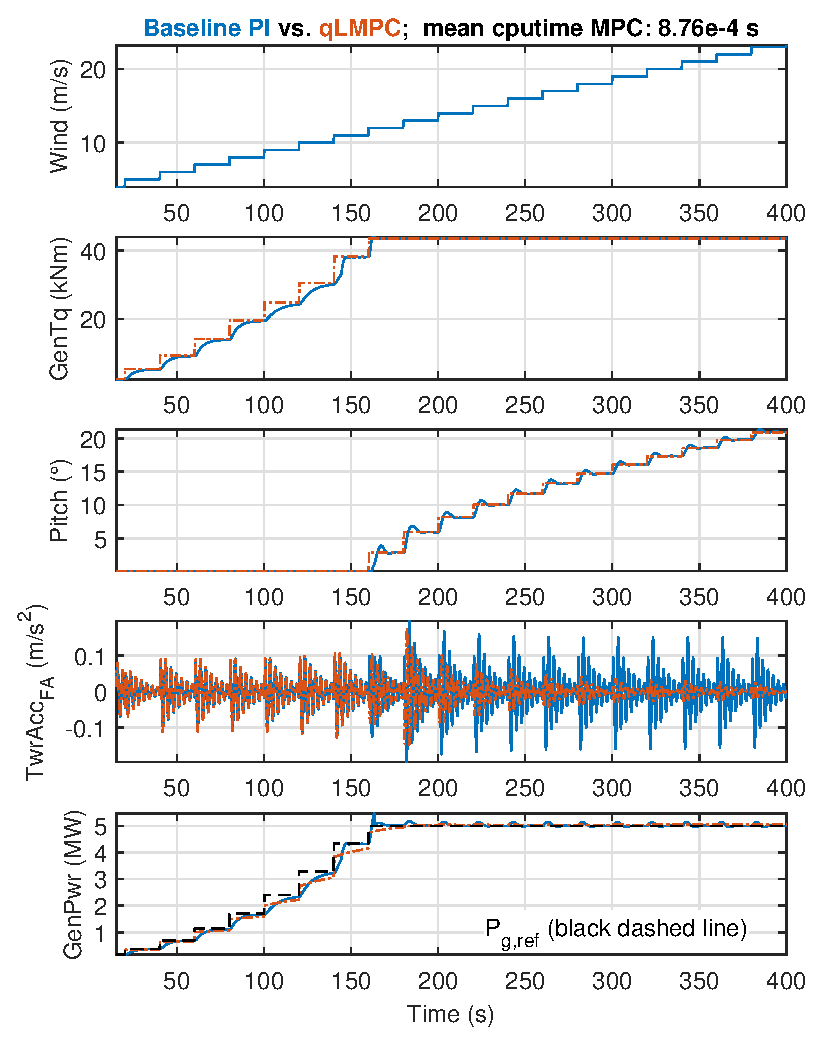
\includegraphics[width=0.485\textwidth]{figures/Figures_ADi/cmpCtrlTimeDomain_All_RefSimulinkClosedLoop_beta.eps}}\hfill 
    \subfloat[Turbulent wind, IEC class B, 18~m/s mean speed]{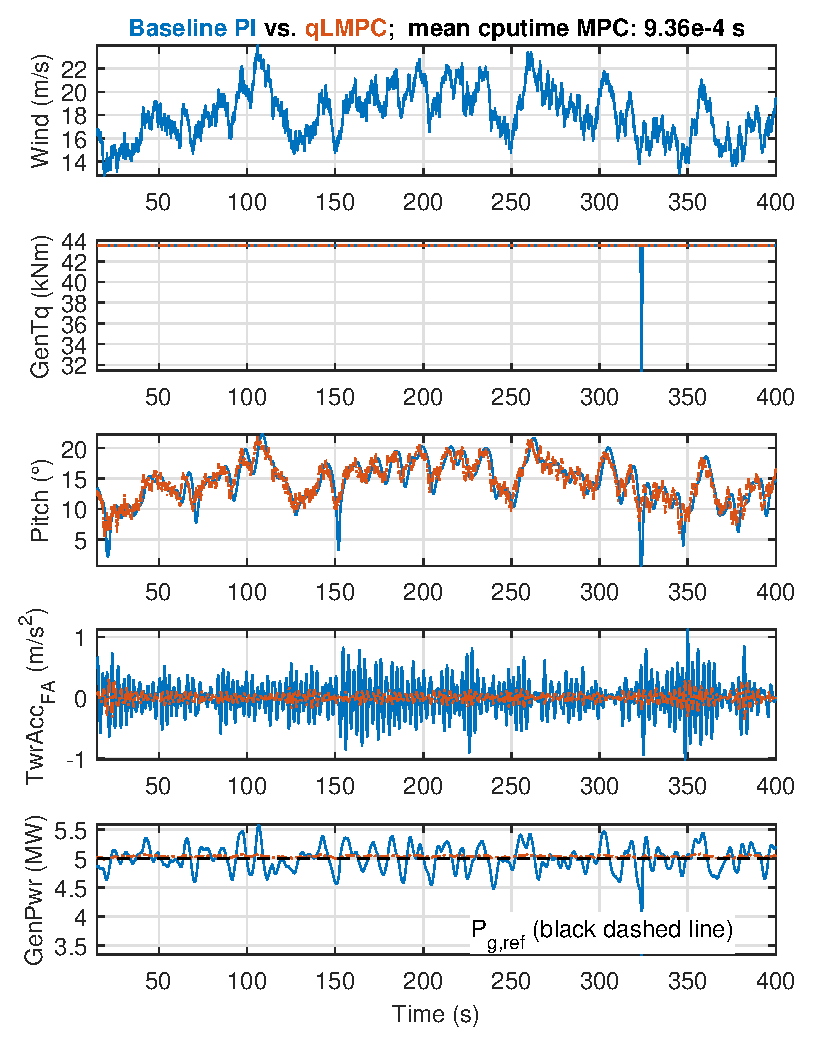
\includegraphics[width=0.485\textwidth]{figures/Figures_ADi/cmpCtrlTimeDomain_All_RefSimulinkClosedLoopNTW18_beta.eps}}\hfill
    %\subfloat[blc blc]{\includegraphics[width=0.31\textwidth]{figures/twoTurbinesGreedyOpt_2d.eps}}
    \caption[Controller comparison: qLPV model with baseline 
    PI controller vs. qLMPC for stepped wind sweep and turbulent wind.]{Controller comparison: qLPV model with baseline 
        PI controller vs. qLMPC for stepped wind sweep and turbulent wind (18\,m/s mean, IEC turbulence 
        class B (14\,\%)).  PI control (blue line), qLMPC (red line) and power reference (black dashed line). Displayed signals: wind speed, control inputs, tower fore-aft
        accelerations, and power output.}
    \label{fig:CtrlCmpMdlSweep}
\end{figure}

 The QP is solved using a linear complementary problem formulation with Lemke's algorithm \cite{cisneros2020velocity}, which enables fast convergence, as real-time capability is a critical requirement for online optimization-based control. Of the 50001 controller cycles at a sampling time of 8\,ms needed for the 400\,s simulation time, only one cycle exceeded the sampling time and only 13 exceeded 2\,ms. The mean CPU time remained considerably below 2\,ms, as shown in the subplot titles of Figure~\ref{fig:CtrlCmpMdlSweep}. These measurements were obtained in MATLAB R2021b on an Intel Core i7-11850H (2.5\,GHz, 8 cores) running Windows 10. Note that for deployment on a physical turbine, a fallback strategy would be required to handle the rare cases where the solver exceeds the sampling time. This was not implemented in this proof-of-concept, but several options exist, such as blending the last available qLMPC solution with the output of the PI feedback controller.

However, the improvements regarding the reduction of tower acceleration and power variance come at the price of higher actuation rate.
Table \ref{tab:ControllerComparisonMerged} summarizes this by displaying the afore mentioned changes in tower fore-aft acceleration and power tracking error as standard deviation for physical interpretability for both the baseline PI controller and the qLMPC algorithm.  
\begin{table}[t]
    \centering
    \caption[Standard deviation comparison: Baseline PI vs.\ qLMPC for stepped wind sweep and
    turbulent wind.]%
    {Standard deviation comparison: Baseline PI vs.\ qLMPC for stepped wind sweep and
        turbulent wind (18\,m/s mean, IEC class B).
        The standard deviations obtained with the PI controller are divided by those obtained with the qLMPC; quotients above~1 indicate improvement.} %In the turbulent wind case, both controllers operate at rated   generator torque throughout, resulting in zero torque rate standard  deviation for both
    \label{tab:ControllerComparisonMerged}
    \begin{tabular}{l rr}
        \toprule
        {Standard Deviation of} & {Stepped wind sweep} & {Turbulent wind} \\
        {Signal (unit)} & \multicolumn{2}{c}{std PI / std qLMPC =  ratio} \\
        \midrule
        Tower fore-aft acceleration ( m/s$^2$) & $0.06 / 0.03 = 1.77$ & $0.17 / 0.07 = 2.31$ \\
        Power tracking error (kW) & $169.01 / 146.26 = 1.16$ & $56.68 / 14.68 = 3.86$ \\
        Generator torque rate (kNm/s) & $0.63 / 2.36 = 0.27$ & $0 / 0 = {-}$ \\
        Blade pitch rate (\textdegree/s) & $0.22 / 0.81 = 0.27$ & $0.51 / 3.60 = 0.14$ \\
        \bottomrule
    \end{tabular}
\end{table}
%
%\\begin{tablenotes}
 %   \small
%    \item In the turbulent wind case, both controllers operate at rated 
%    generator torque throughout, resulting in zero torque rate standard 
%    deviation for both.
%\end{tablenotes}
%
Ratios above~1 indicate improvement, confirming the qLMPC reduces both tower loading and power tracking error.  But the standard deviation in rates in blade pitch increase, for the turbulent wind test case even considerably so. There is also a decrease in generator torque observed for the stepped wind test case. In the turbulent wind case, both controllers operate at rated generator torque throughout, resulting in zero torque rate standard  deviation for both. As more improvement in power variance was observed for the above rated turbulent wind, the following discussion focuses on this case.

For the results of this proof-of-concept, visualized in Figure~\ref{fig:CtrlCmpMdlSweep}, no penalty is placed on pitch actuator movement, and the pitch rate limit is set to 13\textdegree/s, which is a relatively high value. Figure~\ref{fig:CtrlCmpRates} shows the results of six test runs with different pitch rate limits: three with the baseline PI controller and three with the qLMPC algorithm. The effect of different pitch rates on the PI controller is depicted in Figure~\ref{fig:CtrlCmpRates}(a), and on the qLMPC design in Figure~\ref{fig:CtrlCmpRates}(b). The selected pitch rate limits of 4\textdegree/s, 8\textdegree/s, and 13\textdegree/s represent a range from conservative to highly responsive actuator capabilities. They were chosen to explore both realistic hardware limitations and the potential performance gains of faster actuation.

The signals shown for both investigated control algorithms are the wind speed, collective blade pitch angle, rotor speed, fore-aft tower acceleration, and generator power. It should be noted that generator torque does not change at all in this above-rated test case and is hence not shown. Under baseline PI control, increasing the pitch rate shows very little effect, as the rotor acts as a filter in this pure feedback design. In contrast, the qLMPC controller shows a considerable difference when only 4\textdegree/s pitch rate is allowed compared to the two higher rates. Allowing a pitch rate of approximately 8\textdegree/s or faster improves rotor speed regulation and reduces both tower movement and power variability by more than a factor of 3. However, it also leads to higher pitch activity.  The qLMPC reduces the variance of rotor speed, tower fore-aft movement, and power output for all rate limits, even at a  4\textdegree/s rate limit. However, the qLMPC benefits from higher pitch rates, as faster pitch response enables better disturbance rejection. The trade-off between actuator activity on the one hand and load reduction and smoother power output on the other is ultimately a design decision, which may also vary over the turbine's lifetime as the pitch bearings age.

\begin{figure}[h]
    \subfloat[Baseline PI controller]{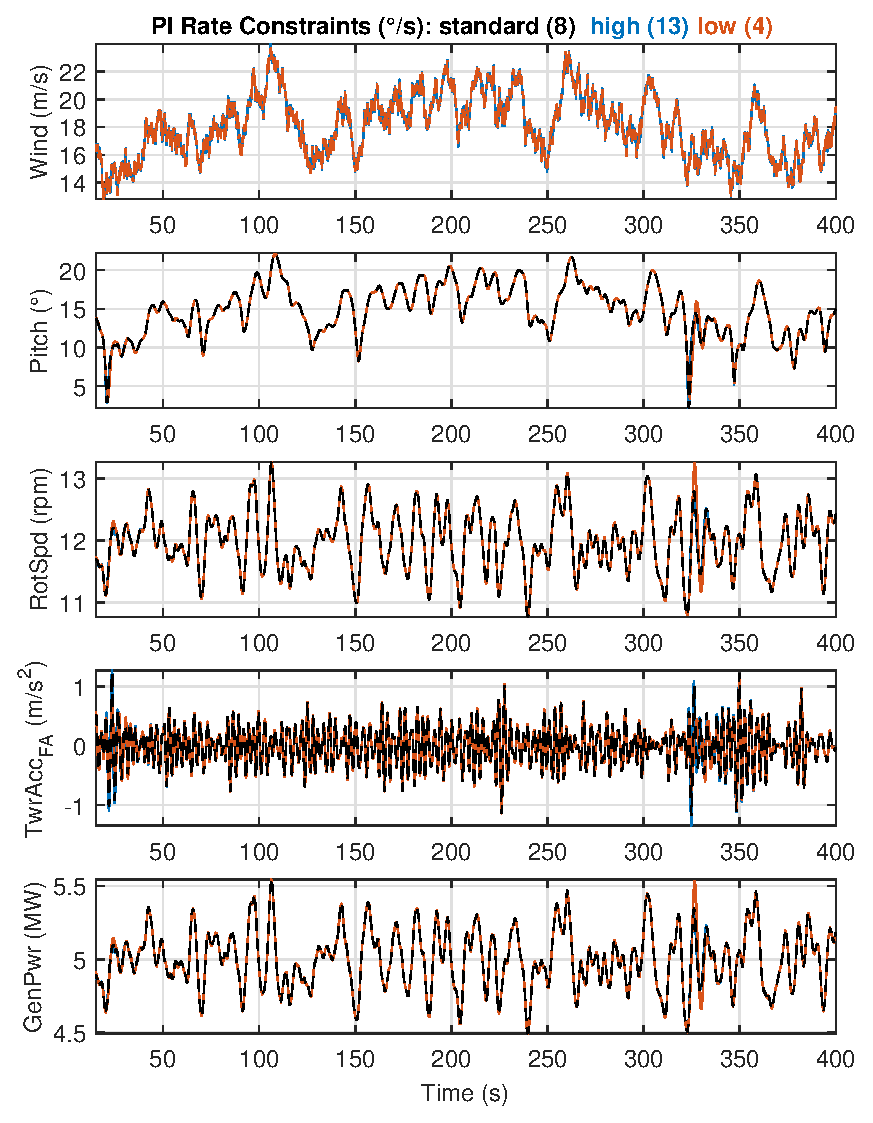
\includegraphics[width=0.485\textwidth]{figures/figDirConstr1/cmpTimeDomain_All5PINewLim.eps}}\hfill 
    \subfloat[qLMPC algorithm]{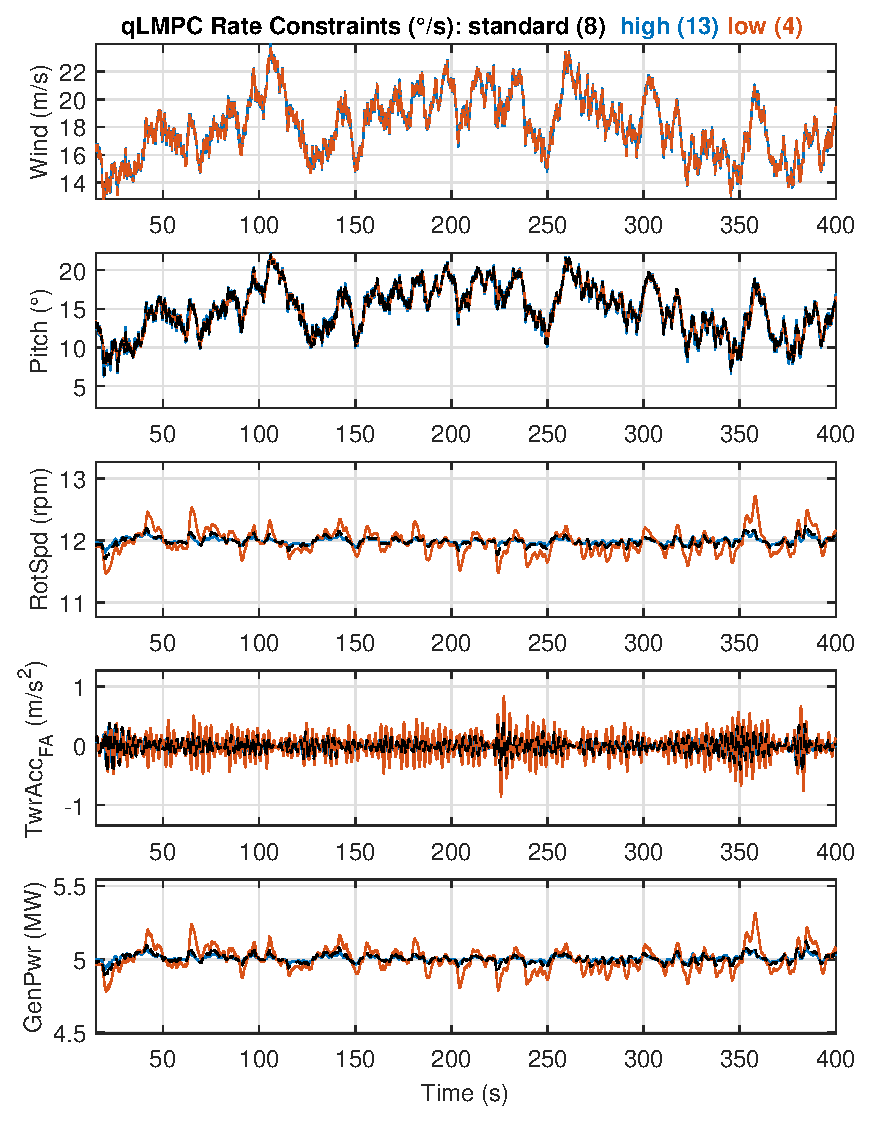
\includegraphics[width=0.485\textwidth]{figures/figDirConstr1/cmpTimeDomain_All5MPCNewLim.eps}}\hfill
     \caption[Controller comparison: Baseline PI and qLMPC with different pitch rate limits.]{Controller comparison: Baseline PI and qLMPC with different pitch rate limits for turbulent wind (18\,m/s mean, IEC turbulence  class B (14\,\%)). Rate limits: Standard 8\textdegree/s~(black line), high 13\textdegree/s~(blue line), and low 4\textdegree/s~(red line)). Displayed signals: wind speed, pitch, states, and power.}
    \label{fig:CtrlCmpRates}
\end{figure}

The standard deviations of the pitch derivative, the rotor speed, the tower fore-aft acceleration and the generated power for Figure~\ref{fig:CtrlCmpRates} are summarized in Table~\ref{tab:stddev_unified}.

\begin{table}[htbp]
    \centering
    \caption[Standard deviation comparison: Baseline PI vs.\ qLMPC for turbulent wind with different pitch rate limits.]%
    {Standard deviation comparison: Baseline PI vs.\ qLMPC
        for turbulent wind with pitch rate limits. The PI controller is largely insensitive to the rate limit
        whereas the qLMPC uses higher rates for less rotor speed, tower movement and
        power variation. Values in brackets show the ratio to the standard
        (8\,\textdegree/s) baseline PI value.}
    \label{tab:stddev_unified}
    \begin{tabular}{ll rrr}
        \toprule
        & & \multicolumn{3}{c}{Rate limit (\textdegree/s) (ratio to PI at 8\,\textdegree/s)} \\
        \cmidrule(lr){3-5}
        Controller & Signal & low: 4\textdegree/s & standard: 8\textdegree/s & high: 13\textdegree/s \\
        \midrule
        \multirow{4}{*}{PI}
        & Tower fore-aft acc.\ (m/s$^2$) & 0.32 (1.03) & 0.33 (1.00) & 0.34 (0.97) \\
        & Generated power (kW) & 200.26 (0.99) & 197.62 (1.00) & 197.32 (1.00) \\
        & Rotor speed (rpm) & 4.57 (0.99) & 4.51 (1.00) & 4.50 (1.00) \\
        & Blade pitch rate (\textdegree/s) & 1.21 (1.06) & 1.28 (1.00) & 1.34 (0.96) \\
        \midrule
        \multirow{4}{*}{qLMPC}
        & Tower fore-aft acc.\ (m/s$^2$) & 0.21 (1.57) & 0.11 (3.00) & 0.08 (4.12) \\
        & Generated power (kW) & 78.37 (2.52) & 30.72 (6.43) & 19.63 (10.07) \\
        & Rotor speed (rpm) & 1.79 (2.52) & 0.70 (6.44) & 0.45 (10.02) \\
        & Blade pitch rate (\textdegree/s) & 1.84 (0.70) & 3.11 (0.41) & 3.88 (0.33) \\
        \bottomrule
    \end{tabular}
\end{table}

The application of the proposed velocity-based qLMPC concept significantly reduces tower movements and minimizes power output fluctuations. As noted at the start of this section, DEL reduction is not directly a qLMPC objective. However, it will be shown in Section~\ref{subsection: IPCResults} and~\ref{subsec:ComparisonWindTurbineControlDesigns} that the reduced tower movement also results in considerably reduced Damage Equivalent Loads (DELs) and the corresponding values are included in comparisons with other control schemes in the Figures~\ref{fig:EvalCrit1} and~\ref{fig:CtrlCompAll}.

The performance improvement comes at the cost of requiring accurate wind information, either obtained through expensive sensors such as lidars or through wind estimations. A purely feedback-based improvement over standard collective pitch control is individual pitch control, which uses blade root moments and rotor azimuth position as additional feedback signals and is already widely deployed in commercial turbines. This approach is widely investigated in both theoretical studies and field tests and has proven to be an effective strategy, either as an alternative or in addition to MPC, to further reduce mechanical loads. While its primary focus is on reducing blade loads, a reduction in tower loads is also possible, as will be discussed in the next section.

\section{Individual Pitch Control Design and Application}\label{section:Individal Pitch PI Control}
Individual Pitch Control (IPC) is a control technique designed to mitigate cyclic loads on wind turbine blades by independently adjusting the pitch angle of each blade. These cyclic loads primarily result from wind shear, i.e., the increase in wind speed with altitude due to reduced surface friction farther from the ground. Additional causes of load imbalances include wind turbulence, gusts and tower shadow effects. These effects lead to asymmetric aerodynamic loading, causing blade movements out of the rotor plane and inducing what are referred to as out-of-plane bending moments at the blade roots. The flapwise and edgewise blade root bending moments are measured directly, for example via strain gauges. The out-of-plane bending moments are then calculated from these measured signals. They occur at specific multiples of the rotor's rotational frequency, commonly referred to as $n\text{P}$ frequencies, e.g., $1\text{P}$ and $2\text{P}$ correspond to once and twice per revolution, respectively. It is important to avoid or damp these frequencies because they can excite the turbine's natural structural modes, leading to resonant oscillations that significantly accelerate mechanical fatigue and reduce component lifespan.

The turbine blade movement can be decomposed into three primary directions relative to the blade itself, which can be measured by sensors: flapwise, which is perpendicular to the rotor plane if the blade is not pitched, edgewise within the rotor plane, and torsional twisting along the blade’s axis. Flapwise and edgewise movements can be transformed into the blade movement within the rotor plane and perpendicular to the rotor plane. The latter movements generate the aforementioned out-of-plane moments. These moments serve as feedback for IPC. IPC effectively targets and suppresses these loads by transforming the blade root moments from the rotating to the stationary rotor coordinate system, augmenting them using a controller, and then re-transforming them back into the rotating frame before applying the adjustments to the blade pitch signals.

The block diagram in Figure~\ref{fig:BlockIPC} illustrates the IPC architecture. It shows the main components of the system, including the controller, which is divided into the power controller and the IPC controller, highlighted in red. The figure also displays the NREL 5MW wind turbine, the pitch actuator, and the torque actuator.
\begin{figure}[ht]
    \centering
    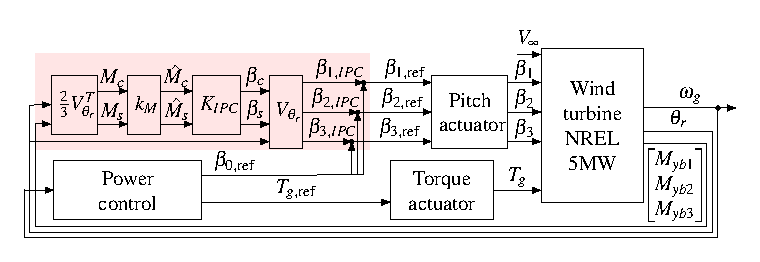
\includegraphics[width=0.9\textwidth,trim={0 0cm 0cm 0.3cm},clip]{figures/Figures_ADi/turbineCtrlBetaIPCcl.pdf}
    
     \caption[Block diagram closed-loop wind turbine control structure with IPC PI added to the baseline PI controller.]{Block diagram of the closed-loop wind turbine control structure with IPC PI (highlighted in red) added to the baseline PI controller.}
    \label{fig:BlockIPC}
\end{figure}
In this work, PI controllers are utilized rather than full PID architectures. This choice is consistent with the NREL 5MW baseline controller provided in FAST. Furthermore, numerical optimization using fminsearch for controller tuning yielded derivative gains near zero. This suggests that for the investigated load cases, the derivative action provided negligible performance improvements while potentially increasing high-frequency actuator wear due to wind turbulence noise

The three blade pitch angles $\beta_1$, $\beta_2$, and $\beta_3$ are the outputs of the pitch actuators corresponding to the references $\beta_{1,\text{ref}}$, $\beta_{2,\text{ref}}$, and $\beta_{3,\text{ref}}$. These references are the sum of the collective reference signal $\beta_{0,\text{ref}}$ from the power controller and the respective IPC adjustments $\beta_{1,\text{IPC}}$, $\beta_{2,\text{IPC}}$, and $\beta_{3,\text{IPC}}$.
%
As before, the power control loop sets the collective pitch reference $\beta_{0,\text{ref}}$ as well as the generator torque reference $T_{g,\text{ref}}$, based on feedback from the generator speed $\omega_g$.
%
These IPC adjustments are derived from the measured out-of-plane blade root bending moments $M_{yb1}$, $M_{yb2}$, and $M_{yb3}$ and the position of the first blade $\theta_{r}$, also called the rotor position or rotor azimuth. The blade root moments are transformed from the rotating into the stationary rotor coordinate system by a multiplication with the matrix $2/3 V^T_{\theta_{r}}$. The back-transformation before applying the control signals onto the rotating blades is done with a multiplication with the matrix $V_{\theta_{r}}$. The underlying method for these coordinate transformations, known as multiblade coordinate transformation, and the design of $V_{\theta_{r}}$ is explained in detail in the following section.

\subsection{Multiblade Coordinate Transformation} \label{sec:MBC}
Multiblade coordinate transformation (MBC) enables the conversion of dynamic loads from the rotating coordinate system, defined by the azimuth angle $\theta_{r}$, to a fixed tower coordinate system. Specifically, load components at the rotation frequency are transformed via the MBC to quasi-static loads. Hence, MBC allows for a more accurate assessment of the loads acting on the turbine tower and other non-rotating components. Applying MBC to convert the rotating blade root flap moments into a fixed coordinate system for a three-bladed wind turbine results in the matrix notation %Therefore, MBC facilitates an optimal calculation of the reference control signal.
\begin{equation} \label{eq:MBC}
    \left[ \begin{array}{c}
        M_0\\
        M_c\\
        M_s
    \end{array} \right] = \frac{2}{3}
    \left[ \begin{array}{ccc}
        1/2 & 1/2 & 1/2\\
        \cos(\theta_{r}) & \cos(\theta_{r} + \frac{2\pi}{3}) & \cos(\theta_{r} + \frac{4\pi}{3})\\
        \sin(\theta_{r}) & \sin(\theta_{r} + \frac{2\pi}{3}) & \sin(\theta_{r} + \frac{4\pi}{3})
    \end{array} \right]
    \left[ \begin{array}{c}
        M_{yb1}\\
        M_{yb2}\\
        M_{yb3}
    \end{array} \right], 
\end{equation}
with  $M_{ybi}$ as the out-of-plane root moment of the $i^{\text{th}}$ blade as inputs and the moments in the non-rotating system as outputs, with these moments being the symmetric load moment $M_0$, pitch moment $M_c$ and yaw moment $M_s$, as visualized in Figure~\ref{fig:BlockIPC}. The pitch and yaw moments are used to calculate two cyclic control signals $q_c$ and $q_s$, i.e., $\beta_c$ and $\beta_s$ for IPC. 
The control signal $q_i$ of the $i^{\text{th}}$ blade is calculated via the second and third columns of the inverse MBC transformation i.e. the inverse of the matrix from Equation~(\ref{eq:MBC}) %, is then used to calculate 
\begin{equation} \label{eq:inverseMBC}
    \left[ \begin{array}{c}
        q_1\\
        q_2\\
        q_3
    \end{array} \right] = 
    \underbrace{\left[ \begin{array}{ccc}
            \cos(\theta_{r}) &  \sin(\theta_{r})\\
            \cos(\theta_{r} + \frac{2\pi}{3}) &  \sin(\theta_{r} + \frac{2\pi}{3})\\
            \cos(\theta_{r} + \frac{4\pi}{3}) &  \sin(\theta_{r} + \frac{4\pi}{3})
        \end{array} \right]}_{V_{\theta_{r}}}
    \left[ \begin{array}{c}
        q_c\\
        q_s
    \end{array} \right],
\end{equation}
where the signal $q_i$ denotes $\beta_{i,\text{IPC}}$ in IPC for the $i^{\text{th}}$ blade. %In Section~\ref{sec:CombinedIPC-TrailingEdgeFlapControl} the same matrix multiplication is once again applied to the $i^{\text{th}}$ flap.
 Note that the transpose of the matrix $V_{\theta_{r}}$ from equation~(\ref{eq:inverseMBC}), multiplied by $2/3$, is equal to the last two rows of the MBC matrix, see also \cite{ossmann2017load}. In the context of this work, and as is common in related literature, see e.g.~\cite{he2018combined}, the pitch and yaw moments $M_c$ and $M_s$ are controlled via $q_c$ and $q_s$ independently, i.e., any remaining coupling following the MBC transformation between $q_c$ and $M_s$ as well as $q_s$ and $M_c$ is neglected. As the wind turbine dynamics can be modeled as a LTI system after transforming rotor blade dynamics into a fixed coordinate system, using MBC from equation~(\ref{eq:MBC}), a simple, intuitive control approach is adopted. Two separate SISO controllers, one for the blade pitch and one for the yaw moment, respectively, are designed to reduce the transformed moments $M_c$ and $M_s$. In this work, the same controller parameters are used, resulting in three parameters to be tuned for this PI controller. Similar to the IPC implementation, only PI controllers were investigated as the inclusion of a derivative component did not yield gains significantly different from zero during the tuning process. Note that the moment $M_0$, corresponding to the rotor-induced drive shaft torque and influencing generator speed and power, is controlled separately by the baseline power controller and is not used in the IPC controls. 
moments are addressed with the IPC control loop. The 2P loads are addressed with the trailing-edge flap controller making use of the fast flap dynamics.

\subsection{IPC Parameter Optimization} \label{subsection: IPCOptCriteria}
The primary objective of wind turbine control is to minimize the levelized cost of energy (LCoE) by balancing the conflicting goals of maximizing power output while minimizing mechanical loads, particularly damage equivalent loads (DELs) on the tower and blades. This work leverages controller optimization criteria originally used by \cite{hoffmann2018load}, where a standard baseline wind turbine controller, comprising generator torque control and a gain-scheduled PI pitch controller, is augmented with an IPC PI controller and tower damping. The optimization criteria in a multi-objective optimization were the minimization of blade and tower DELs, actuator dynamics, power tracking error, and standard deviation.

The PI design presented in this thesis is a two step approach: In a first step, initial values for the integral and proportional gain of the IPC are found via a grid search. Following this, the three PI parameters are optimized with the Nelder-Mead simplex algorithm implemented in MATLAB’s \textit{fminsearch.m} to reduce the blade DEL. The initial values of the proportional and integral gain are the ones previously found with the grid search. The derivative initial value is set to zero. % and found to diverge very little from it. 
For both steps of the controller tuning, the grid search as well as for the optimization, the quality of an IPC controller are quantified via the decrease in blade root DEL. The cost function $J$ to be minimized by the IPC is the maximum of the DEL of the three blades: 
\begin{equation} \label{eq:costFunIPC}
    J = \text{min}(\text{max}\left(\text{DEL}_{bi,\text{IPC}}/\text{DEL}_{\text{bi,\text{baseline}}}\right)), \quad \text{i} \in {1,2,3} 
\end{equation} %\underset{\Delta u}{\text{minimize }}
with $\text{DEL}_{bi,\text{IPC}}$ derived from the blade flapwise root DEL accumulated over a simulation run with IPC normalized by $\text{DEL}_{\text{bi,\text{baseline}}}$ with only the baseline controller active.
%\subsection{Optimization and evaluation criteria}
To evaluate and quantify the impact of an IPC controller's performance, four additional criteria are calculated, previously used in \cite{hoffmann2018load} as optimization criteria in a multi-objective optimization approach: The tower DELs derived from the bending moments at the base of the tower, the mean and standard deviation of the generated power and the additional power requirements of the actuator due to individual pitch control. The evaluation criteria can be summarized as below.

\subsubsection*{Load Criteria: Blade $C_{\text{DEL},b} = J$ and tower DEL $C_{\text{DEL},t}$}
Reducing the blade DEL is the main incentive for using IPC to decrease the Power Spectral Density (PSD) at 1P. A reduction at the 1P frequency does not influence the tower DEL, however, finding a controller that decreases the peak at 1P tends to also result in a lower PSD for a wider frequency range including the peak at 2P. Thus, a small decrease in the tower DEL is also achieved although this criterion is not included in the objective function. In Section~\ref{sec:CombinedIPC-TrailingEdgeFlapControl} it will be discussed that decreasing the PSD at the 2P frequency via the flaps does decrease the tower DELs futher. 

The blade DEL is calculated as
\begin{align*}
     \Tilde{D}_{b} &=   \frac{1}{3}  \sum_{n_b=1}^3\sum_{i=1}^{k}\left(l_{bn_b,i}  M_{yb,i}^{m_{\text{GFRP}}}\right)
\end{align*}
with $l_{b}$ as the recorded stress level and $M_{yb,i}$ as the out-of-plane root bending moment measured at the $k$ samples of a simulation run for all blades.  The Wöhler coefficient of carbon is $m_{\text{GFRP}} =10$. Note that because of this even exponent, both negative and positive moments with large amplitudes increase the damage value.
The equation for the damage criterion of the three blades is:
\begin{align*}
    C_{\text{DEL},b} &=  \Tilde{D}_{b,\text{IPC}}/\Tilde{D}_{b,\text{baseline}}  %\frac{1}{\Tilde{D}_{b,\text{baseline}}} 
\end{align*}
%
with  $\Tilde{D}_{b,\text{IPC}}$ and $\Tilde{D}_{b,\text{baseline}}$ as the recorded blade damage for the two controllers for the same test case. 

The equation for the tower damage criterion is
\begin{align*}
    C_{\text{DEL},t} &= \frac{1}{\Tilde{D}_{t,\text{baseline}}} \cdot
    \left[ \sum_{i=1}^{k_{t}} \left( l_{t,i} \cdot M_{xt,i}^{m_{\text{Steel}}} \right) + 
    \sum_{i=1}^{k_{t}} \left( l_{t,i} \cdot M_{yt,i}^{m_{\text{Steel}}} \right) \right]
\end{align*}
with $\Tilde{D}_{t,\text{baseline}}$ as the recorded tower damage for the CPC-PI controller for the same test case, $m_{\text{Steel}} =4$ the Wöhler coefficient of steel, $M_{xt,i}$ and $M_{yt,i}$ the tower moments at the top around the longitudinal and lateral axis, respectively,  $l_{t,i}$ the recorded stress level, and $k_t$ the number of data samples.

\subsubsection*{Power Criteria: Mean $C_{\bar{P}}$ and Standard Deviation $C_{\delta_P}$}
As the annual energy production should not suffer from IPC, the generated power is compared as well. It was found that the power production loss and variance increase is at 0.1\% and hence negligible. The power variance is important for the network stability, especially in small networks. The effect of the IPC controller is found to be nearly negligible. Similarly to the DEL criteria, the power criteria are normalized by the results obtained with the CPC-PI controller
\begin{align*} %\label{eq:CP}
    C_{\bar{P}} =  \bar{P}_{\text{g,\text{IPC}}}/ \bar{P}_{\text{g,\text{baseline}}}  \quad\text{and}\quad C_{\delta P} =  \delta P_{g,\text{IPC}}/ \delta P_{g,\text{baseline}}.
\end{align*} 

\subsubsection*{Actuator Power Criterion $C_{\text{Act}}$}
This is the only criterion for which an increase is unavoidable, due to the additional movement of the blades required by the IPC controller. The actuator power criterion is normalized as:
\begin{equation} \label{eq:CAct}
    C_{\text{Act}} = \frac{P_{\text{Act}, \text{IPC}}}{P_{\text{Act}, \text{baseline}}}.
\end{equation}
where \( P_{\text{Act}, \text{baseline}} \) is the reference actuator power of the baseline controller. The actuator power is defined as the mean product of the blade pitch rate $\dot{\beta}$ and the actuator pitch moments $M_{bz}$:
\begin{equation} \label{eq:CAct_calc}
    P_{\text{Act}, \text{IPC}} = \frac{1}{3} \sum_{b=1}^3 \overline{|\dot{\beta} \cdot M_{bz}|}.
\end{equation}
The controller parameters are optimized for different pitch rate limits, as the optimization objectives described above converge to different optima depending on the actuator constraints. As in the analysis of the qLMPC controller behavior, the rates are set to 4\textdegree/s, 8\textdegree/s, and 13\textdegree/s to investigate settings ranging from very conservative to highly agile. In the following results section, a comparative analysis in both the time and frequency domains is presented to illustrate how these trade-offs affect structural loads, power output, and actuator behavior, i.e., the quantitative controller objectives described in this section.

\subsection{Results} \label{subsection: IPCResults}
Figure~\ref{fig:timeseriesIPC} visualizes the results of the baseline CPC and two IPC controllers, with parameters optimized for 4\,m/s and 13\,m/s pitch rate limits. In all test cases, the turbine is excited with the same wind signal, which has a mean wind speed of 16\,m/s and corresponds to turbulence class B. The first subplot shows this wind speed signal, which is also used for controller tuning during the optimization. The subsequent plots display generator torque, pitch angles, rotor speed, tower fore-aft acceleration, generator power, and blade root out-of-plane moments.
\begin{figure} [H]
    \subfloat[Pitch rate limit 4\textdegree/s]{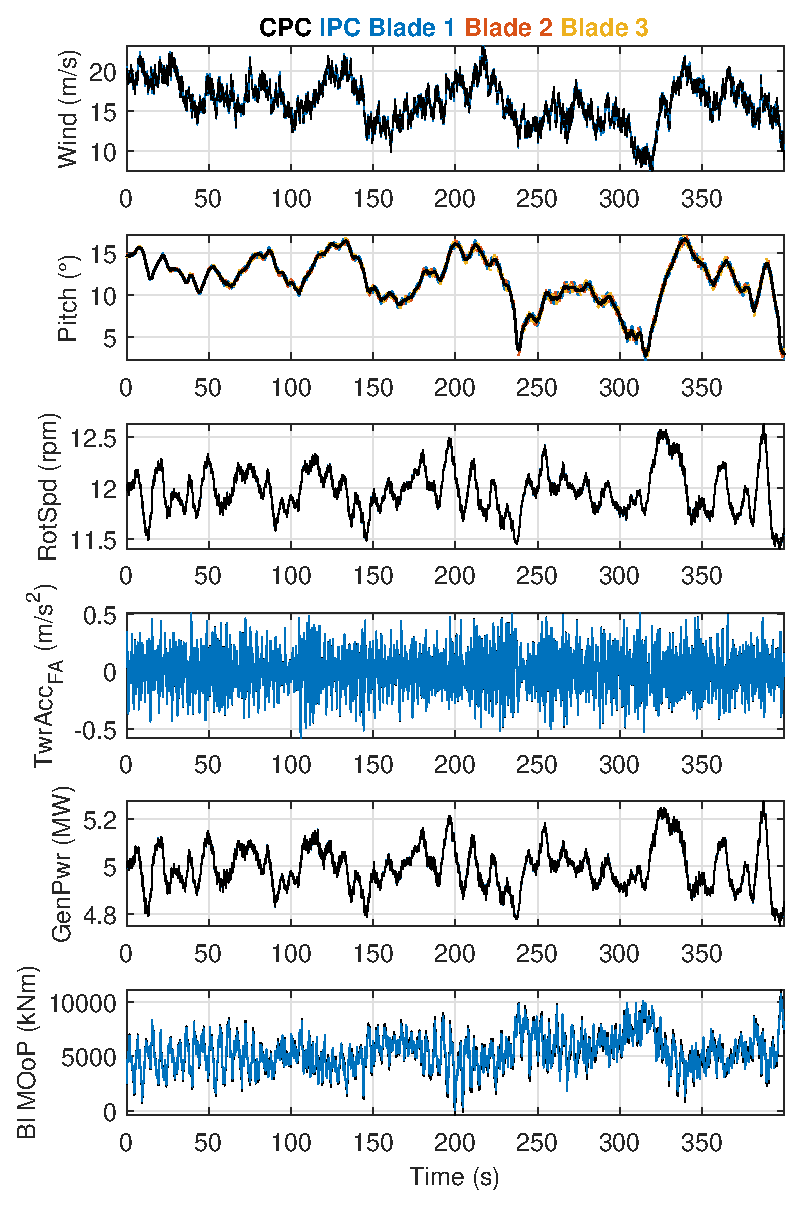
\includegraphics[width=0.49\textwidth]{figures/figures_WESC25/fig00a_Timeseries1.eps}}\hfill 
    \subfloat[Pitch rate limit 13\textdegree/s]{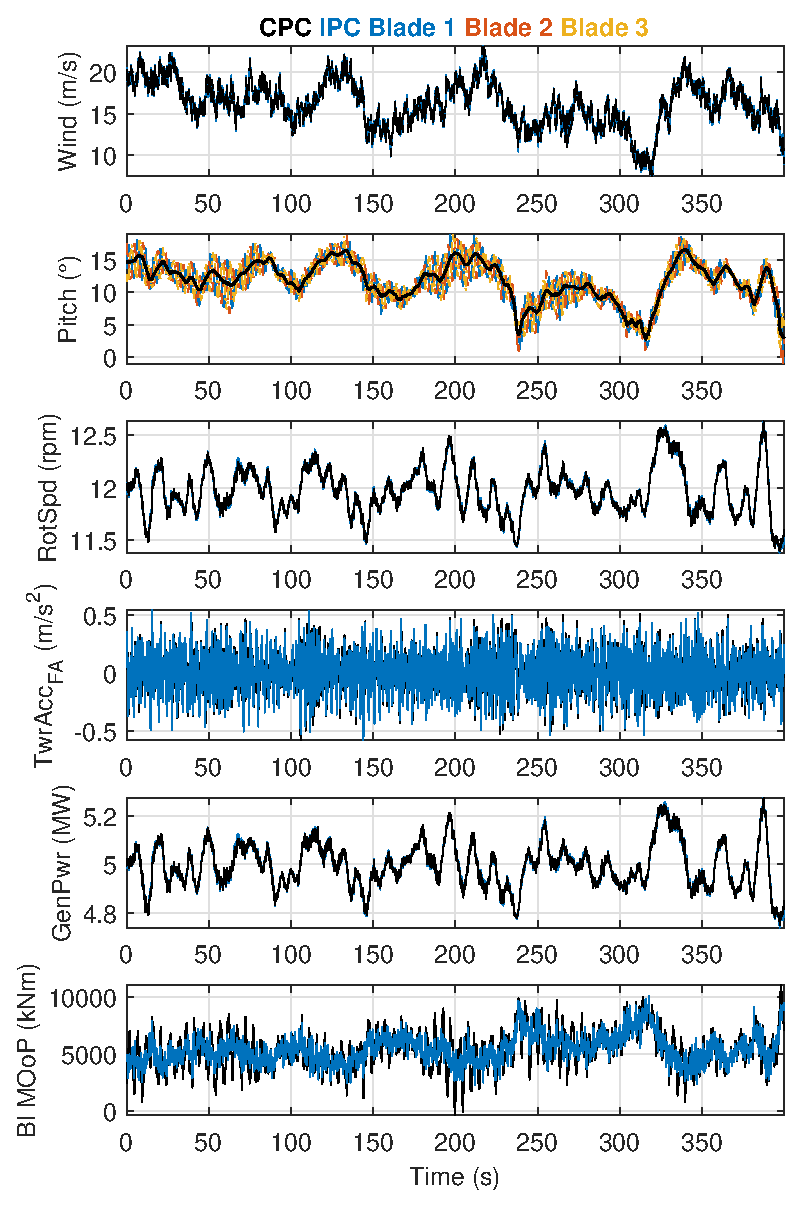
\includegraphics[width=0.49\textwidth]{figures/figures_WESC25/fig00a_Timeseries3.eps}}\hfill
    \caption[Controller comparison: Baseline and IPC PI with different pitch rate limits.]{Controller comparison: Baseline (black) and IPC PI (blue, red and yellow lines pitch signals, blue all other signals) with different pitch rate limits for turbulent wind (16\,m/s mean, IEC turbulence class B (14\,\%)). Rate limits: Low (4\textdegree/s) and high (13\textdegree/s~) for IPC, standard  (8\textdegree/s) for baseline PI. Displayed signals: wind speed, pitch, states, power, and out-of-plane blade root moments.}
    \label{fig:timeseriesIPC}
\end{figure}

Generator torque, rotor speed, and generator power remain nearly unchanged between the two IPC configurations and the baseline PI CPC. This is expected, as the power control logic, which sets the generator torque and collective pitch demand, is identical across all controllers. Differences in tower fore-aft motion are also nearly imperceptible in this time series. The most notable differences appear in the pitch signals, which oscillate at the 1P frequency in both IPC cases, and in the resulting blade root out-of-plane moments. At the lower pitch rate limit of 4\textdegree/s, shown in the left column, the IPC controller has also only a limited effect on the blade root out-of-plane moments. In contrast, the right column, corresponding to the very high pitch rate limit of 13\textdegree/s, shows that the individual pitch actuators significantly reduce the variance of the out-of-plane moments, thereby improving load reduction on the blades. A very slight decrease in tower fore-aft acceleration is also detectable at this rate limit. 
As expected, increasing the allowable pitch rate enhances the effectiveness of the IPC controller in alleviating structural loads.   

Figure~\ref{fig:PSDIPC} shows the Power Spectral Density (PSD) of the blade root out-of-plane moment to visualize and explain the gradual improvement with increasing pitch rate for all three test cases. The black line represents the baseline CPC. The blue line, representing IPC with a 4°/s rate limit, reduces the 1P peak by 87\%, while the red line, representing IPC with an 8°/s rate limit, further lowers it, achieving a significant 98\% reduction. At the 2P frequency, the blue line shows a slight increase compared to the baseline, while the red line effectively lowers the 2P peak. As expected, the 8°/s rate limit offers better load reduction across both 1P and 2P frequencies. The controller tuned with the rate limit set to 13°/s, depicted as a yellow line, decreases the 1P and 2P peaks even more. 
\begin{figure}[h]
    \begin{center}
        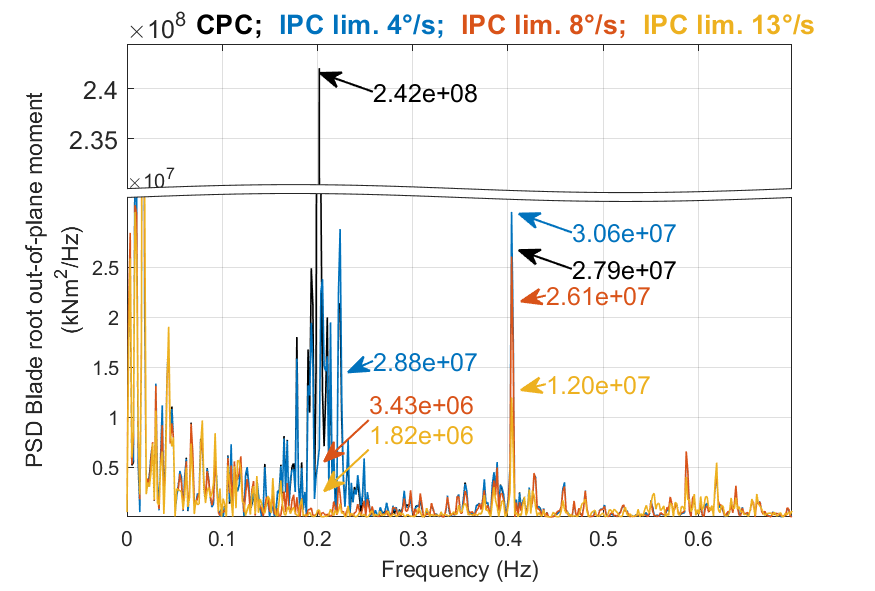
\includegraphics[width=0.6\textwidth]{figures/figures_WESC25/fig02_PSDroot_breaky_ratecomp.png}
        \caption[Controller comparison: Power Spectral Density of blade root out-of-plane moment of baseline PI with 8\textdegree/s rate limit, IPC with 4°/s,  8°/s, and 13°/s rate limit]{Controller comparison: Power Spectral Density of blade root out-of-plane moment of baseline PI (black) with 8\textdegree/s rate limit, IPC with 4°/s rate limit (blue),  8°/s rate limit (red), and 13°/s rate limit (yellow)}
        \label{fig:PSDIPC}
    \end{center}
\end{figure}

Table~\ref{tab:stddev_unified_IPC} summarizes the standard deviation of the signals shown in Figure~\ref{fig:timeseriesIPC} for IPC rate limits of 4°/s, 8°/s, and 13°/s. The baseline PI values are completely insensitive to the rate limit as the pitch rates stay below the limit of 4°/s, they are constant across all three cases. For the states and power output, the introduction of IPC also does not produce any observable effect. Even the tower fore-aft acceleration, which appeared marginally improved under visual inspection at 13°/s, shows a ratio of 1.00 throughout. The pitch rate standard deviation increases unavoidably for the IPC test cases: by 27\% at the most restrictive limit of 4°/s, and by factors of 3.61 and 5.74 at 8°/s and 13°/s respectively. In contrast, the blade root out-of-plane moment is reduced by 5\%, 21\%, and 23\% across the three limits, consistent with the spectral load reductions at 1P and 2P visible in Figure~\ref{fig:PSDIPC}.
\begin{table}[htbp]
    \centering
   \caption[Standard deviation comparison: Baseline PI vs. IPC for turbulent wind with 
   different pitch rate limits.]{Standard deviation of IPC blade pitch rate and blade root 
       OoP moment for turbulent wind with different pitch rate limits. Values in brackets show 
       the ratio to the PI baseline. Tower fore-aft acceleration, generated power, and rotor 
       speed standard deviations are identical to the PI baseline across all rate limits and are 
       therefore omitted. PI baseline standard deviations differ only for the blade pitch rate (0.54\,\textdegree/s)
       and blade root OoP moment (1628.85\,kNm).}
    \label{tab:stddev_unified_IPC}
    \begin{tabular}{l rrr}
        \toprule
        & \multicolumn{3}{c}{ IPC rate limit (\textdegree/s) (ratio to CPC rate limit (\textdegree/s))} \\
        \cmidrule(lr){2-4}
        Signal & low: 4\textdegree/s & standard: 8\textdegree/s & high: 13\textdegree/s \\
        \midrule
        Tower fore-aft acc.\ (m/s$^2$)  & 0.17 (1.00) & 0.17 (1.00) & 0.17 (1.00) \\
        Generated power (kW)             & 91.59 (1.00) & 91.78 (1.00) & 91.97 (1.00) \\
        Rotor speed (rpm)                & 2.09 (1.00) & 2.09 (1.00) & 2.10 (1.00) \\
        Blade pitch rate (\textdegree/s) & 0.69 (1.27) & 1.95 (3.61) & 3.09 (5.74) \\
        Blade root OoP moment (kNm)      & 1546.19 (0.95) & 1282.12 (0.79) & 1248.97 (0.77) \\
        \bottomrule
    \end{tabular}
\end{table}


Figure~\ref{fig:EvalCrit1} shows the evaluation criteria, described in Section~\ref{sec:quasi-LPVTurbineModel}, for the PI IPC and the qLMPC CPC under varying pitch rate limits for the test case pictured in Figure~\ref{fig:timeseriesIPC}.  The criteria are obtained by normalizing all objectives by the values achieved with the PI
baseline for the same test case. The bar plot illustrates five performance metrics: blade
and tower damage equivalent loads $C_{\mathrm{DEL},b}$ and $C_{\mathrm{DEL},t}$, mean
power tracking error $C_{\bar{P}}$, power output standard deviation $C_{\delta_{P}}$, and
pitch actuation energy $C_{\text{Act}}$. 
Note that the standard deviation metrics used previously are insensitive to the amplitude and frequency distribution of load cycles.
DELs, which are computed via rainflow counting, capture these effects directly and are
therefore used as the performance metric for mechanical loads throughout the remainder of
this section. With IPC, blade root DELs are reduced by 3\%, 14\%, and 15\% depending on the pitch
rate limit, while tower DELs decrease by 3\% and 5\% at the two higher rate limits.
%\begin{figure}[htbp]
%    \begin{center}
%        \subfloat[IPC]{\includegraphics[width=0.48\textwidth]{figures_WESC25/afig01_IPCbar.eps}}\hfill
%        \subfloat[MPC]{\includegraphics[width=0.48\textwidth]{figures_WESC25/afig03_MPCbar.eps}}\hfill
%        \caption{Power criteria, actuator energy, blade and tower DEL of PI IPC and MPC CPC
%            controllers.}
%        \label{fig:EvalCrit1}
%    \end{center}
%\end{figure}

\begin{figure}[h]
    \begin{center}
        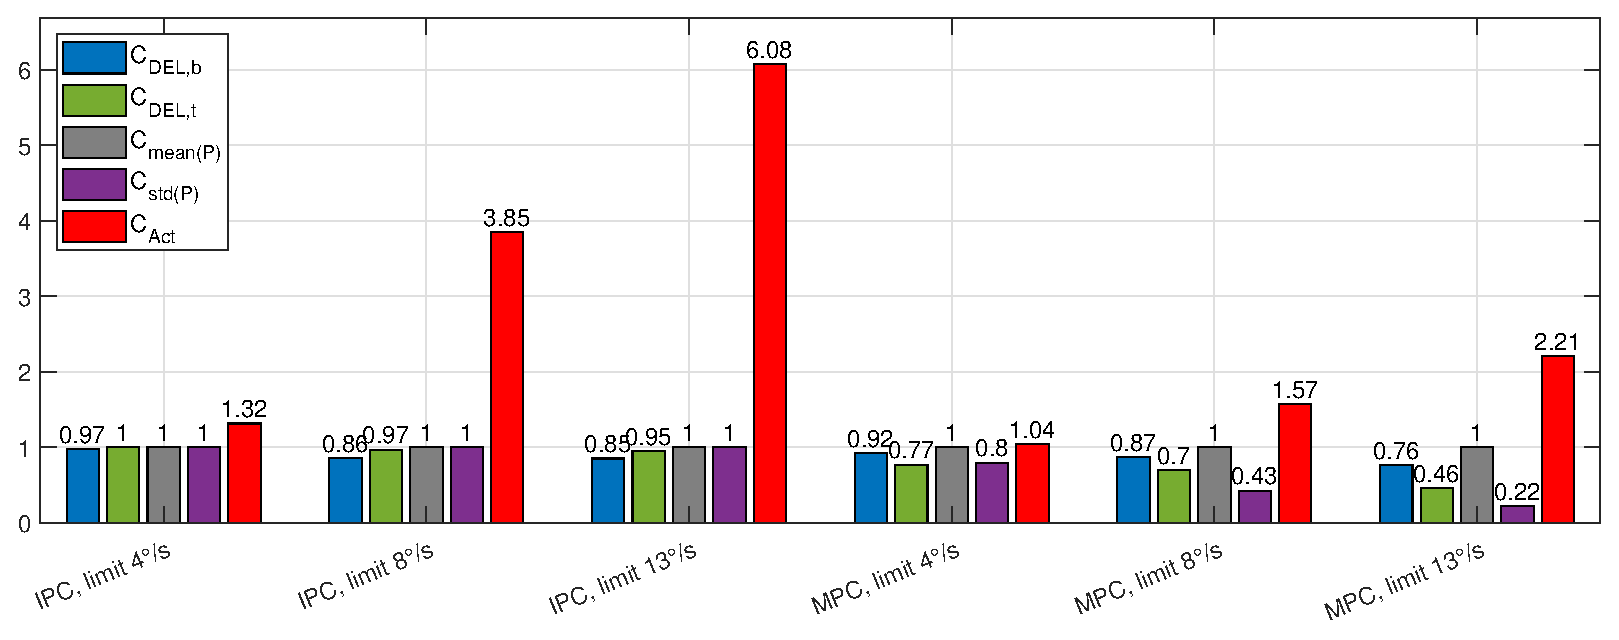
\includegraphics[width=0.95\textwidth]{figures/figures_WESC25/afig01_IPCMPCbar.eps}
        \label{tabCtrlcomp}
            
         \caption[Wind turbine controller evaluation criteria for qLMPC and IPC with different pitch rate limits for turbulent wind] {Wind turbine controller evaluation criteria  qLMPC and IPC  for turbulent wind (16\,m/s mean, IEC turbulence class B (14\%)). Criteria are tower base and blade DELS, power mean and standard deviation, and pitch actuator power.}
        \label{fig:EvalCrit1}
    \end{center}
\end{figure}



The power tracking and variance performance $C_{\bar{P}}$ and $C_{\delta_{P}}$ remain
identical to the baseline. The progressive improvement of the load reduction metrics
$C_{\mathrm{DEL},b}$ and $C_{\mathrm{DEL},t}$ with higher pitch rate limits comes at the
cost of increased pitch activity, as reflected in the strongly increasing $C_{\text{Act}}$
values of 1.32, 3.85, and 6.08. The qLMPC controller shows the same trade-off between actuator activity and load
reduction. Since the individual blade loads driven by wind shear across the rotor are not
directly addressed by collective pitch control, the stronger load reduction is observed in
the tower DEL, which is substantially reduced by 23\%, 30\%, and 54\% across the three
rate limits, reflecting the qLMPC's effectiveness in attenuating tower fore-aft motion.
While the blade DEL reductions are smaller, they are at 8\%, 13\%, and 24\% still either
larger or nearly equal to those obtained at the same pitch rate limits with IPC. As with
IPC, the power tracking performance $C_{\bar{P}}$ is not changed. However, due to the
reduction in rotor speed deviations achieved with the qLMPC, the power standard deviation
$C_{\delta_{P}}$ decreases markedly at higher rate limits, consistent with the previously
reported smoother power output. At higher pitch rate limits, the qLMPC shows an increase
in pitch activity, but significantly less so than for the IPC controller at the same
limits.

IPC was shown in this section to reduce blade loads, with the amount of reduction progressively increasing with higher pitch rate limits, at the cost of increased actuator energy. It was also shown to decrease tower loads to a certain degree. 
However, the qLMPC, discussed in the previous section, reduces tower loads more effectively, as it directly controls the collective pitch to lower thrust fluctuations. Notably, the qLMPC also achieves comparable or 
better blade load reductions than IPC, even though it does not explicitly target 
individual blade loads and based on this single time series analysis, the qLMPC appears to 
be the more effective single controller overall. However, it should be taken into account that the performance of the MPC strongly depends on the model quality as well as the agreement between estimated wind and true wind. Obviously, the performance of IPC also depends on the quality of the blade root out-of-plane measurements. Nevertheless, IPC Pi controllers are at the moment more widely accepted as a relatively simple method for larger turbines to decrease blade loads. An MPC IPC approach could reduce blade and tower loads even further, but the combined actuator demand may become 
unacceptably high.

While this section focused on load mitigation through individual pitch control, further 
improvements can be achieved by including additional actuators. As blade sizes continue to 
increase, additional actuation devices integrated into the blade structure might become 
necessary. The following section introduces a turbine model enhanced 
with trailing edge flaps on the rotor blades, enabling combined IPC and flap control for 
more effective high-frequency load reduction.

\section{Combined IPC Trailing Edge Flap Control Design and Application}
\label{sec:CombinedIPC-TrailingEdgeFlapControl}

Building on the previous investigations into IPC and qLMPC strategies, this section focuses on a combined control approach that incorporates both IPC and Trailing Edge Flaps (TEF). By including TEFs in the rotor blades as supplementary actuation surfaces, additional degrees of freedom become available for targeted load mitigation, particularly at higher frequencies. This combination of individual pitch and trailing edge flap control is referred to as IPC-TEFC or Active Aerodynamic Load Control (AALC). AALC is defined as the integrated use of multiple aerodynamic control surfaces to actively reduce structural loads and improve turbine performance. By coordinating both individual blade pitch adjustments and trailing edge flap deflections, AALC provides enhanced load mitigation compared to each method alone. This section presents the model formulation for incorporating TEFs into the wind turbine dynamics and evaluates a combined IPC–TEFC strategy across Region~III operation. The controller design is based on an optimization framework that considers multiple wind conditions and turbulence intensities to ensure good performance over the whole operating range. Following the methodology outlined in the report \cite{osterwinter2019load1}, the approach is validated using a comprehensive set of verification wind fields to assess load reduction, power preservation, and actuator demand. This work has been published in \cite{dittmer2024combined}.


\subsection{TEF Simulation Model} %bonnie_jonkman_openfastopenfast_2022 OpenFAST2023
As before, the OpenFAST simulation software is used to investigate the benefits of combining individual pitch and trailing-edge flap control. The NREL 5MW wind turbine model is modified to implement controllable trailing-edge flaps on the rotor blades. The original NREL 5MW model without TEF serves as a reference for analyzing the aerodynamic effects of these modifications on the simulated operation of the turbine. 
\subsubsection*{Rotor Blade Geometry and Aerodynamics}
The rotor blades of the NREL 5MW turbine are defined by eight distinct cross-sectional profiles distributed along the blade length, as illustrated in Figure~\ref{subfig:TEF1}, and comprise 19 nodes, each with specific geometric profile shapes. At the root, cylindrical profiles connect to the rotor hub, accommodating high bending moments and pitch adjustments. The profiles transition from the DU series, developed at Delft University of Technology, near the root to the NACA64 profile in the outer 29\% of the blade, characterized by decreasing thickness towards the tip. The blade's aerodynamic efficiency is further refined by varying the profile depth and orientation at each node.

The blade section with trailing-edge flaps, which covers the whole NACA64 blade section, is marked in red. The flap-to-blade chord ratio amounts to 20\%. The aerodynamic model of the blade enhanced with TEF requires input data on lift, drag, and pitching moment coefficients for all profiles across various blade angles of attack and a variety of flap deflection angles. The three main factors influencing these aerodynamic properties are surface roughness, Mach number, and Reynolds numbers. The OpenFAST simulation neglects surface roughness variations due to contaminants. The airflow is assumed to be incompressible with a Mach number of 0.25 at the blade tip. Interpolating between different polars is implemented in OpenFAST based on a user-defined parameter, by default the Reynolds number. In this work the interpolation between polars is performed based on the flap positions. As only one interpolation parameter can be defined, the Reynolds number distribution depicted in Figure~\ref{subfig:TEF1} is used for all wind speeds. Care was taken to model the distribution of Reynolds numbers along the rotor blade at this wind speed as realistically as possible. Realistic Reynolds numbers for rotor blades range from one to eight million are obtained from an OpenFAST simulation with turbulence class A at a mean wind speed of 12\,m/s. The OpenFAST aerodynamic models of the rotor blades are extended with additional airfoil polars based on this distribution.  % with the numbers obtained via an OpenFAST simulation run with a wind file from the optimization data set, with turbulence class A and the meand wind speed at 12\,m/s.
\begin{figure}[h]
    \centering
    \includegraphics[width=0.6\textwidth]{Images_Torque24/fig01_RE.eps}\hspace{0pc}%
    \begin{minipage}[b]{0.95\textwidth}\caption[ Span-wise distribution of Reynolds numbers Re at wind speed $V_{\infty} = 12$\,m/s]{\label{subfig:TEF1} Span-wise distribution of Reynolds numbers Re at wind speed $V_{\infty} = 12$\,m/s (from OpenFAST simulation) and blade geometry with cylinder, DU40, DU35, DU30, DU25, DU21 and NACA64 profiles with TEF location covering the NACA64 section marked in red.}
    \end{minipage}
\end{figure}

\subsubsection{Polar Calculation with xflr5 and XFOIL}
The aerodynamic coefficients of rotor blade profiles for the TEF enhanced blades are calculated using the programs xflr5 and XFOIL, see \cite{drela1989xfoil}. XFOIL uses a higher-order panel method to analyze and design airfoil profiles, incorporating variables like Reynolds number, Mach number, and a transition criterion for calculating the shift from laminar to turbulent flow. The turbulence degree of the incoming flow determines the appropriate transition criterion value, with the default value set at 9, approximating a median turbulence level as per XFOIL's documentation. For fluid properties, standard sea-level values from the International Standard Atmosphere (ISA) are used. The aerodynamic coefficients for the respective profiles are calculated based on the Reynolds numbers selected from Figure \ref{subfig:TEF1}. The coefficients generated by xflr5 and XFOIL are not directly suitable for wind turbine simulation as AeroDyn15 requires coefficients over an angle of attack range from -180\textdegree{} to +180\textdegree. Since XFOIL's panel methods yield accurate results only up to the point of flow separation, the polars are extrapolated to cover the entire required angle range. This extrapolation is performed using the AirfoilPrep preprocessor developed by NREL, applying the Viterna method for extrapolating polars, see for details e.g.~\cite{gasch2011wind}. %on Viterna's calculation process 
Additionally, corrections are made to account for three-dimensional flow effects caused by the rotor blade's rotation. Factors like Coriolis and centrifugal forces increase the maximum lift coefficients in the inner rotor areas. These 3D effects are corrected using functions integrated into AirfoilPrep. Figure \ref{subfig:TEF2} illustrates the extrapolated and corrected lift and drag coefficients over the angle of attack for rotor blade profiles with different flap angles. 

Figure \ref{subfig:TEF2}\,(a) shows that a positive flap deflection leads to an increase in lift coefficients $c_l$ and hence in lift. A positive flap deflection is defined as the flap moving backwards with respect to the chord line of the local blade profile with an undeflected flap. The point of maximum lift coefficient shifts to a smaller angle of attack than with a neutral flap position. A negative flap deflection has the opposite effect. The lift coefficients are reduced and the point of maximum lift coefficient shifts to higher angles of attack. This corresponds to the expected effects of different trailing-edge flap deflections on the lift. 

Figure~\ref{subfig:TEF2}\,(b) visualizes the drag coefficient. The curves of the drag coefficient $c_d$ appear smooth and physically meaningful for angles of attacks above -27\textdegree. Note that there is a sudden reversal of the vertical staggering of the polars below this value. There is neither a physical explanation for this effect, nor is any discontinuity observed for the rotor profile without trailing-edge flap. It can be assumed that the extrapolation method does not work optimally for profiles with flaps at these high TEF angles that would lead to flow separation and stall.  However, this can be disregarded as the range of TEF angles of attack in the simulations in the outer area of the rotor blades do not exceed -27\textdegree\ during normal operation. As this study uses OpenFAST v3.2.1, no additional code needs to be added for the TEF inclusion, unlike earlier studies that leveraged previous versions of FAST. The obtained coefficients are summarized in a text file, which is included as a parameter in the Airfoil Information section of the AeroDyn15.dat file of the NREL 5MW model available in the Git repo \cite{GitRepoCodeAALC}. %NACA64_A17_Flap.dat
%
\begin{figure} [h]
    \subfloat[Lift coefficient $c_{l}$]{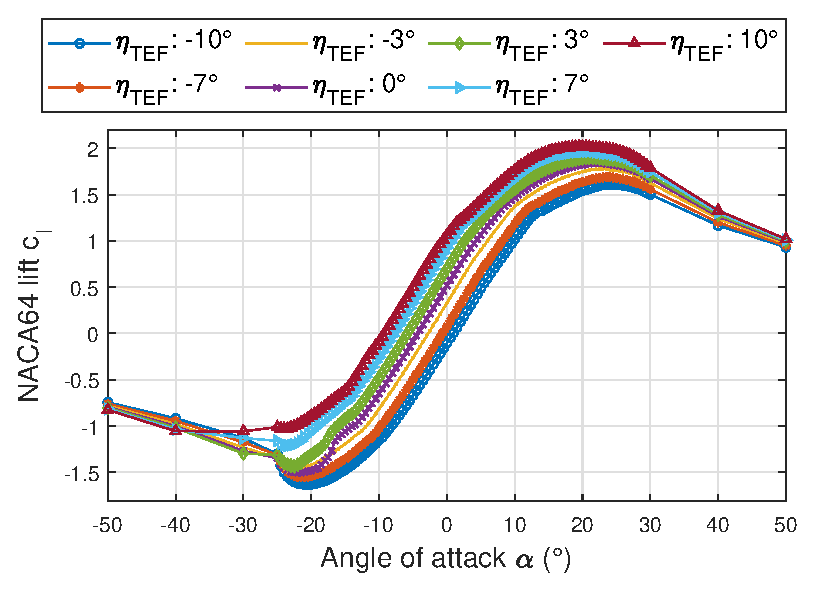
\includegraphics[width=0.485\textwidth]{figures/Images_Torque24/fig01_Cl1out.eps}}\hfill 
    \subfloat[Drag coefficient $c_{d}$]{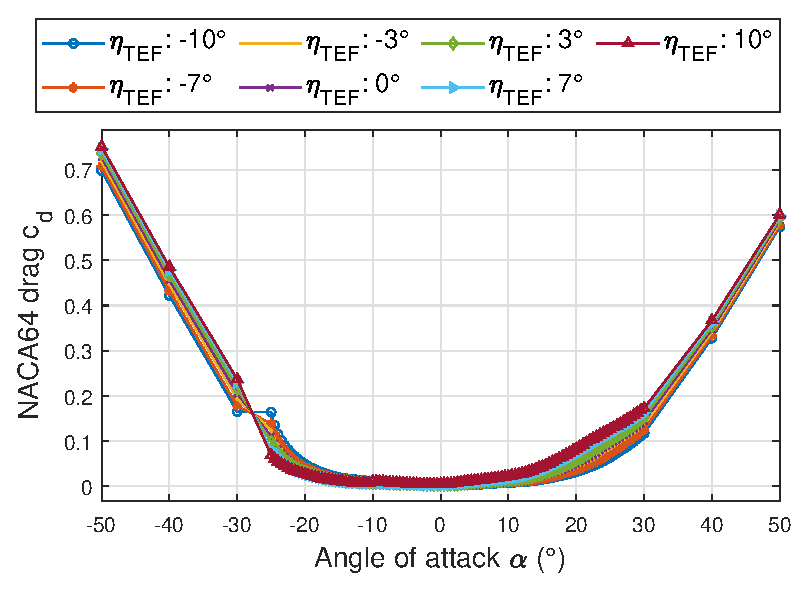
\includegraphics[width=0.485\textwidth]{figures/Images_Torque24/fig01_Cd1out.eps}}\hfill
    %\subfloat[blc blc]{\includegraphics[width=0.31\textwidth]{figures/twoTurbinesGreedyOpt_2d.eps}}
    \caption{Lift and drag coefficients at different TEF angles $\eta_{\text{TEF}}$ and different blade angles of attack $\alpha$.}
    \label{subfig:TEF2}
\end{figure}
%

\subsection*{Baseline Power Controller} %speed-controlled-pitch-controlled
In order to realistically simulate a modern turbine, a control system controlling rotor speed and generator torque is required, and the same baseline controller described and applied in the previous sections is utilized for that purpose. The aim of the IPC-TEFC is to further decrease the mechanical loads. Note that this load reduction controller using IPC together with TEF-control is an add-on controller to the baseline control system. This is possible as cyclic pitch motions are induced, which are effectively decoupled from the collective pitch motion ensuring the maximum power output above rated wind speed. As before, the implementation of the baseline controller is the power controller available within TU Delft's FASTTool, see \cite{mulders2020wind}. 
%
\subsubsection*{Open-Loop TEF Model Verification with FAST} % with TEF open loop control
The modified NREL 5MW turbine model presented in the previous section is tested in open-loop simulations with regard to the plausibility of the influence of the TEF position on the simulation results. The aerodynamic model of the trailing-edge flap is included. Open-loop control inputs of the TEF deflection angle $\eta$ are analyzed in order to investigate its suitability with regard to the desired DEL reduction. The effects of flap deflections on different parameters relevant to the operational quality of the wind turbine, such as forces and moments as well as power yield, are investigated. Figure \ref{fig:OLdiag} shows a block diagram to illustrate the control structure used for these verification tests, with the eight inputs, i.e., the seven control inputs and the wind of the selected test case $V_{\text{TC}}$ as a disturbance. The actuators for the pitch angle adjustment of the rotor blades are modeled as first order transfer function with position and rate limitations. The influences of different TEF positions for steady-state operating conditions are discussed in Section~\ref{subsec:ResultsTEF}. 
% For a sensitivity study of the flaps with regard to their influence on the blade root flapping moments, we refer to \cite{osterwinter2019load1}.
\begin{figure}[h]
    \centering
    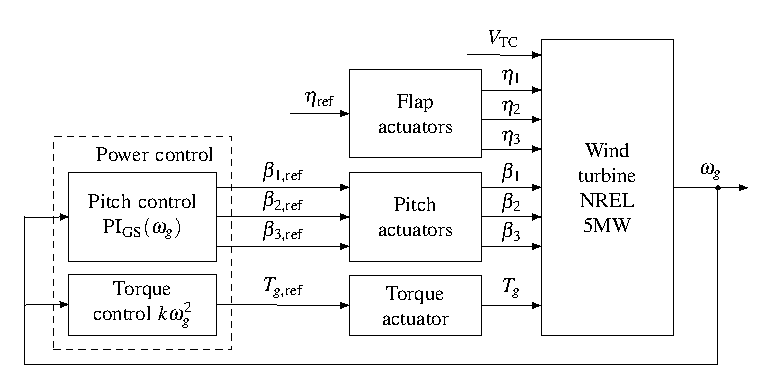
\includegraphics[width=0.95\textwidth, trim=0 0 0 13, clip]{figures/Images_Torque24/blockdiagram_OL_latex_tau2.pdf}\hspace{2pc}%
    \begin{minipage}[b]{0.95\textwidth}\caption{\label{fig:OLdiag} Block diagram for open-loop TEF verification tests with baseline power control in closed loop and open-loop collective TEF control inputs.}
    \end{minipage} %BlockschaltbildopenLoop1.jpg
\end{figure}

\subsection{IPC-TEFC Implementation}
The main design objective of the presented AALC is the reduction of structural moments, focusing on flapwise blade root bending moments. The overall controller layout is shown in Figure~\ref{fig:CLdiag}. The baseline controller, depicted in Figure~\ref{fig:OLdiag}, is enhanced with IPC, with the individual pitch demand added to the collective pitch reference, as well as TEFC which changes the TEF position. All six AALC control output signals are calculated via MBC, see Section \ref{sec:MBC}, based on the three out-of-plane blade root moments, $M_{yb1}$, $M_{yb2}$, and  $M_{yb3}$, as well as the rotor azimuth $\theta_r$. This section reviews the allocation of IPC and TEFC signals and then discusses the design of these controllers. 
\begin{figure}[h]
    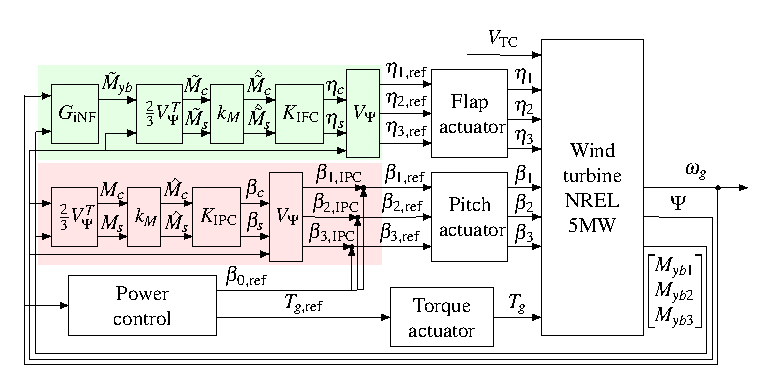
\includegraphics[width=0.95\textwidth]{figures/Images_Torque24/blockdiagram_CL_latex2.pdf}\hspace{2pc}%
    \begin{minipage}[b]{0.95\textwidth}\caption[Block diagram for closed-loop TEF verification tests with baseline power control, individual pitch and TEF closed loop control.]{\label{fig:CLdiag} Block diagram for closed-loop verification tests with baseline power control, individual pitch (highlighted in red) and TEF (highlighted in green) closed loop control.}
    \end{minipage}
\end{figure}
\subsubsection*{IPC and TEFC Control Allocation}
MBC enables the conversion of dynamic loads from the rotating blade coordinate system, defined by the azimuth angle $\theta$, to a fixed tower coordinate system. Specifically, load components in the 1P frequency range are transformed via the MBC to quasi-static loads. Hence, MBC allows for a more accurate assessment of the loads acting on the turbine tower and other non-rotating components. Applying MBC to convert the rotating blade root flap moments into a fixed coordinate system for a three-bladed wind turbine results in the matrix calculation in Equation~\eqref{eq:MBC} Therefore, MBC facilitates an optimal calculation of the reference control signal.

Figure~\ref{fig:CLdiag} denotes $M_{ybi}$ as the flapwise blade root moment of the $i^{\text{th}}$ blade as inputs, and the blade tilt moment $M_c$ and yaw moment $M_s$ in the non-rotating system as outputs. The moments $M_c$ and $M_s$ are used to calculate two cyclic control signals $q_c$ and $q_s$, i.e., $\beta_c$ and $\beta_s$ for IPC, and $\eta_c$ and $\eta_s$ for TEFC. The control signal $q_i$ of the $i^{\text{th}}$ blade is calculated via the inverse MBC transformation in Equation~\eqref{eq:inverseMBC} 
where the signal $q_i$ denotes $\beta_{i,\text{IPC}}$ and $\eta_{i,\text{ref}}$ in IPC and TEFC, for the $i^{\text{th}}$ blade or flap, respectively.  As for the IPC scheme, the tilt and yaw moments $M_c$ and $M_s$ are controlled via $q_c$ and $q_s$ independently, i.e., any remaining coupling following the MBC transformation between $q_c$ and $M_s$ as well as $q_s$ and $M_c$ is neglected. As the wind turbine dynamics can be modeled as a LTI system after transforming rotor blade dynamics into a fixed coordinate system, using MBC from Equation~(\ref{eq:MBC}), a simple, intuitive control approach is adopted. Four separate SISO controllers, two for IPC and TEFC, respectively, are designed to reduce the transformed moments $M_c$ and $M_s$. The system is now over-actuated, i.e., two moments, $M_c$ and $M_s$, need to be mitigated, but four control inputs, $\eta_c$, $\eta_s$, $\beta_c$, and $\beta_s$, are available. This offers the possibility of a frequency separation as a form of control allocation. To achieve this frequency separation of IPC and individual flap control inverse notch filters are implemented in the AALC controller. The 1P loads in the frequency spectrum of the blade root bending moments are addressed with the IPC control loop. The 2P loads are addressed with the trailing-edge flap controller making use of the fast flap dynamics. While modern MIMO controllers, e.g.,  AALC extension of the $H_\infty$ control \cite{ossmann2021field,ossmann2017load} or MPC \cite{dittmer2021velocity}, have the potential to optimize the available control inputs regarding the criteria listed in section \ref{sec:ControllerParameterOptimization} more efficiently, this simple, intuitive CA is selected as the resulting controller does not employ an observer based structure and hence does not require the design of an explicit mathematical plant model.%via strategies such as MPC, LQG or $H_\infty$ control. %Details are elaborated below.

\subsubsection*{Individual Pitch Control for 1P Load Reduction}
The IPC controller $K_{\text{IPC}}$, illustrated in the red part of Figure \ref{fig:CLdiag}, receives the blade root flap moments $M_{yb1}$, $M_{yb2}$, and  $M_{yb3}$ from the rotating coordinate systems, transforming them into fixed coordinate system moments $M_c$ and $M_s$ via MBC without additional filtering. This approach obviates the need for low-pass filtering within the IPC loops, as the actuator models already provide inherent low-pass filtering characteristics. The transformed moments are scaled with $k_M = 10^{-5}$, a value chosen due to the order-of-magnitude difference between the moments and the control angles in units of radians. The scaled moments $\hat{M}_s$ and $\hat{M}_c$ are passed to two identical SISO controllers. These controllers are based on the assumption that the transformed moments become largely independent after the transformation. The LTI nature of the transformed system allows for the potential use of PI controllers. Moreover, for IPC, which focuses on mitigating low-frequency load changes, particularly the 1P loads caused by tower wake effects and wind speed variations, a controller with an integral gain is first tuned manually. The integral component adequately addresses the control requirements by minimizing the steady-state error of the transformed moments and thus effectively targets the minimization of the 1P loads in the rotating coordinate system. This aids in decoupling of the IPC from the TEFC controller, with the TEFC used for controlling higher frequencies. The calculated control signals $\beta_c$ and $\beta_s$ are converted back to the rotating blade coordinate systems via the inverse MBC given in equation~(\ref{eq:inverseMBC}), resulting in the three signals $\beta_{i,\text{IPC}}$. The IPC exclusively calculates individual pitch angle components, avoiding interference with collective pitch angles calculated by the baseline power controller. The pitch angle commands, passed to the pitch actuators, $\beta_{i,\text{ref}}$ are calculated by adding the collective pitch angle command $\beta_{0,\text{ref}}$ to these individual pitch reference signals. The actuator model is implemented as a first order transfer function with time constant $\tau_{\beta}=0.1$ with the angle limited from -2\textdegree{} to 90\textdegree{} and the rate limited from -8\textdegree{}/s to 8\textdegree{}/s. The pitch actuator angles $\beta_i$ are then applied to the OpenFAST NREL 5MW wind turbine model.

\subsubsection*{Trailing-edge Flap Control and Inverse Notch Filter for 2P Load Reduction}
The PI controller for the individual trailing-edge flap control $K_{\text{IFC}}$ is constructed similarly to the IPC, with the MBC and inverse MBC forming central elements, encompassing the two identical SISO controllers for controlling the transformed moments. A key difference is that the blade root flap moment signals are filtered through an inverse notch filter before MBC processing, amplifying selected frequencies
\begin{equation*} \label{eq:Ginf}
    G_{\text{iNF}}(s) = (s^2 +2kDfs +f^2)/ (s^2 +2Dfs +f^2),\quad k=10,\quad D = 0.1
\end{equation*}
with frequency $f$ set as twice the value of the current rotor frequency $f_r$ and s being the Laplace variable. This enhances 2P load amplitudes in the signals, enabling the TEFC to predominantly respond to these loads, thus minimizing mutual influence with the IPC. Post-filtering, the three blade root flap moments $\tilde{M}_{ybi}$ are transformed into the fixed coordinate system via a multiplication with $2/3 V^T_{\theta}$, with the resulting moments $\tilde{M}_{c}$ and $\tilde{M}_{s}$. These are both scaled with $k_m$ to $\hat{\tilde{M}}_c$ and $\hat{\tilde{M}}_s$ . Initially, two proportional controllers are used, with the manually tuned proportional parameter used as a starting point for the optimization of PI controller parameters. The transformed control outputs are then converted back for flap angle adjustments, with flap actuators modeled for a more rapid response than the pitch actuators, aiding in 2P load reduction. The TEF actuator is modeled as a first order transfer function with time constant $\tau_{\eta}=0.05$, with the angle limited from -10\textdegree{} to 10\textdegree{}, and the rate limited from -20\textdegree{}/s to 20\textdegree{}/s.

\subsection*{TEF-IPC Controller Parameter Optimization} \label{sec:ControllerParameterOptimization}
Like the IPC design, the presented AALC design is a two step approach: In a first step, initial values for the integral gain of the IPC and the proportional gain of the TEFC are found via a grid search. Following this, the six AALC PI parameters are optimized with the Nelder-Mead simplex algorithm implemented in MATLAB’s \textit{fminsearch.m} to reduce the blade DEL. Both for the manual controller tuning as well as for the optimization the quality of an AALC controller is quantified via the decrease in blade root DEL. The cost function $J$ to be minimized by the AALC is the maximum of the DEL of the three blades, i.e., the same cost function as provided in Equation~\eqref{eq:costFunIPC}.
To evaluate and quantify the impact of an AALC controller's performance, the same criteria as before are used, which can be summarized as follows:

\begin{itemize}
    \item \textbf{Blade $C_{\text{DEL},b} = J$ and tower DEL $C_{\text{DEL,t}}$:} Reducing the blade DEL is the main incentive for using
    IPC to decrease the PSD at 1P. Load reductions at the 1P frequency does
    not influence the tower DEL, while decreasing the PSD at the 2P frequency via the
    flaps does also decrease the tower DEL. Therefore, a decrease in tower DEL is observed although this criterion is not included in the objective function.  
    \item \textbf{Power mean $C_{\bar{P}}$ and standard deviation $C_{\delta P}$:} The power criteria were also not included in the
    optimization. As the annual energy production is typically not allowed to decrease from AALC,
    the generated power was compared for all test cases above 16\,m/s and it was found
    that the power production loss and variance increase are negligible. % The power
    %variance is important for the stability in small networks. The effect of the AALC controller was found to be nearly negligible.
    \item \textbf{Actuator power $C_{\text{Act}}$:} This is the only criterion for which an increase is
    unavoidable, due to the additional, unavoidable movement of the blade that
    the IPC controller requires. %With the activation of individual pitch control, the pitch actuator power tripled to approximately 4.5 kW for all pitch actuators.
\end{itemize}
Unlike the previously discussed proof-of-concept on IPC and its comparison with qLMPC, not just one wind test signal but an optimization data set with wind of turbulence class~A is created to optimize the PI parameters for each wind speed separately. Another difference from the previous study is that the actuator rate is fixed at 8\textdegree/s. The AALC's effect is analyzed by incorporating five wind speeds in Region~II, from 4\,m/s to 11\,m/s, and nine wind speeds in Region~III, ranging from 12\,m/s to 25\,m/s. Two verification sets are created for the 14 different wind speeds: one with turbulence class~A using a different seed, and one with turbulence class~B. The vertical wind speed distribution is modeled with a power law wind profile to represent wind shear, using an exponent of 0.2. All wind fields are available in the Git repository \cite{GitRepoCodeAALC}, which also includes the code to reproduce all results presented here. 

\subsection{Results} \label{subsec:ResultsTEF}
This section discusses both open loop results, obtained with the simulation set-up depicted in Figure~\ref{fig:OLdiag}, as well as closed loop results, simulated with the control loop from Figure~\ref{fig:CLdiag}. Figure~\ref{fig:OLval} shows the steady state values, at three different TEF angles, of power $P_g$, rotor speed $\omega_r$, rotor thrust $T_r$, and blade pitch angle $\beta_{0}$ for all 14 wind speeds. Simulations at constant wind speeds are run for 660\,s to confirm the validity of the TEF model. Data from the initial 60\,s are excluded to avoid non-physical initialization artifacts and the mean values are calculated for each wind speed.
\begin{figure} [h]
\subfloat[Power and rotor speed]{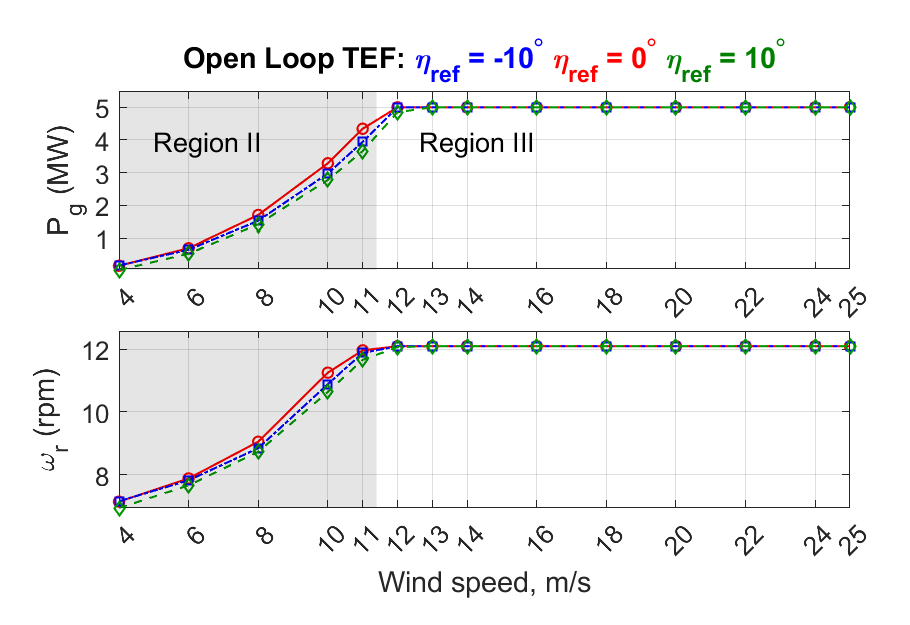
\includegraphics[width=0.485\textwidth]{figures/Images_Torque24/fig06_TEFOL_1.eps}}\hfill 
\subfloat[Rotor thrust and blade pitch]{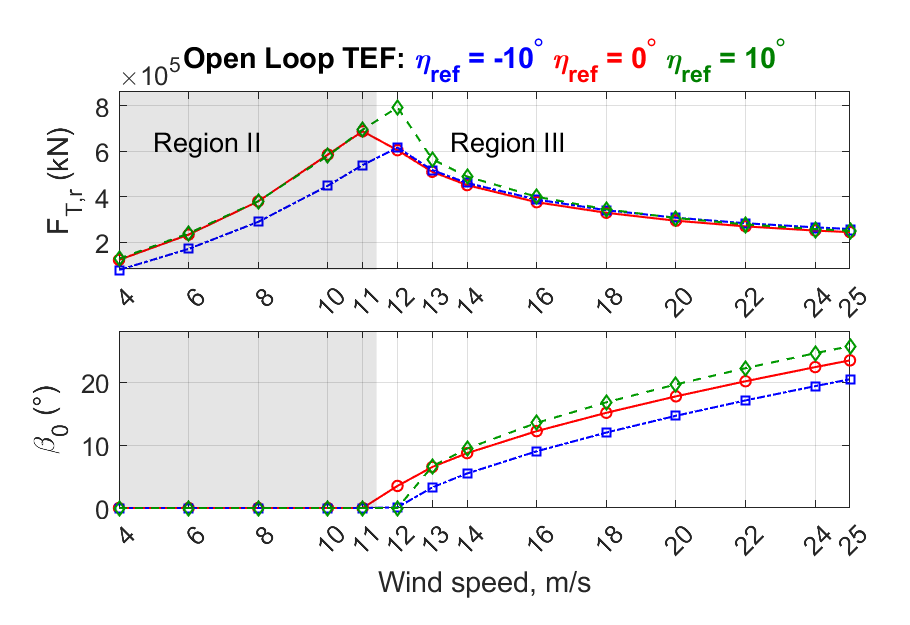
\includegraphics[width=0.485\textwidth]{figures/Images_Torque24/fig06_TEFOL_2.eps}}\hfill
%\subfloat[blc blc]{\includegraphics[width=0.31\textwidth]{figures/twoTurbinesGreedyOpt_2d.eps}}
\caption{TEF open-loop verification, TEF deflection at -10\textdegree{}\,(blue), 0\textdegree{}\,(red), and 10\textdegree{}\,(green).}
\label{fig:OLval}
\end{figure}

%
The simulated power with and without TEF deflections shows the expected power characteristic curve of a wind turbine: In Region~II, both positive and negative flap deflections reduce power \(P_g\) due to decreased aerodynamic efficiency, unlike in Region~III, where the same power output is observed, as the power controller controls the pitch angle once rated wind speed is reached. Adjusting the pitch changes the aerodynamic forces. The control system can therefore maintain nominal power. This also reflects on the rotor speed \(\omega_r\), depicted in the second plot, which is slightly lower in Region~II but unchanged in Region~III. The thrust \(T_r\) in Region~II is decreased by a negative flap angle, while the influence of a positive flap angle on the thrust is negligible: The thrust cannot be increased beyond the neutral flap position due to the limited wind power, which necessarily limits the amount of energy converted into rotational energy. This leads to a dynamic equilibrium where, despite positive flap deflection, the thrust forces remain at levels equivalent to those at the neutral flap position. The second plot in Figure~\ref{fig:OLval}\,(b) shows the blade pitch \(\beta_{0}\), which is lower for a negative and higher for a positive TEF angle, corresponding to the lower and higher thrust force.

Figure~\ref{fig:PSDTEF} shows the power spectral density (PSD) of the blade root bending moment in closed-loop for the first verification data set with a mean wind speed of 16 m/s. 
\begin{figure} [h]
    \subfloat[Baseline (black), IPC (blue), and IFC (green)]{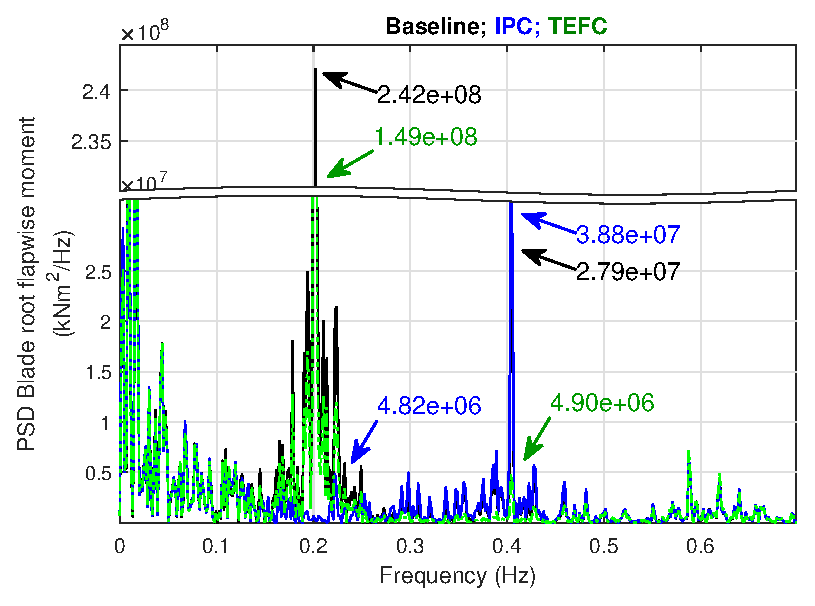
\includegraphics[width=0.485\textwidth]{figures/Images_Torque24/fig02_PSDroot_breaky.eps}}\hfill 
    \subfloat[AALC (red), and AALC optimized (pink)]{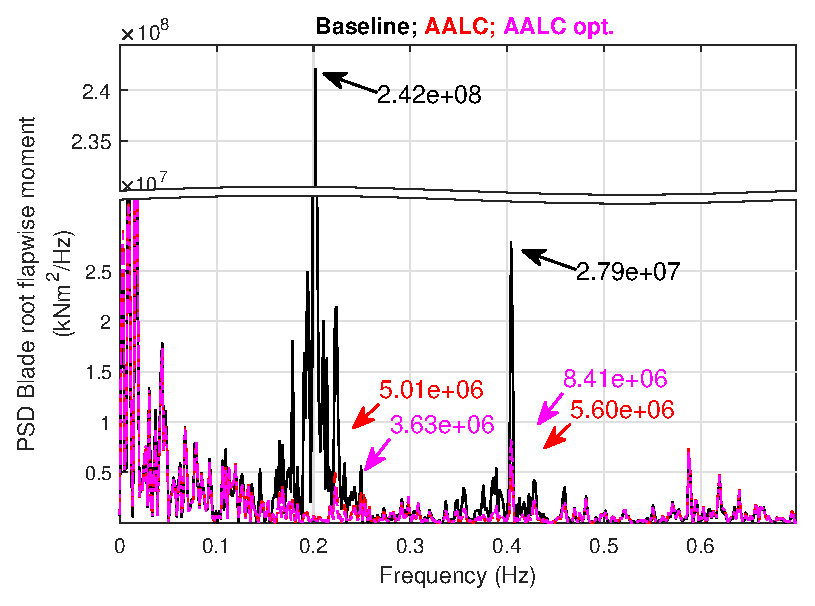
\includegraphics[width=0.485\textwidth]{figures/Images_Torque24/fig02_PSDroot_breaky1c.eps}}\hfill
    %\subfloat[blc blc]{\includegraphics[width=0.31\textwidth]{figures/twoTurbinesGreedyOpt_2d.eps}}
    \caption{Power Spectral Density of optimization set signals, turbulence class A, with mean wind speed 16~m/s.}
    \label{fig:PSDTEF}
\end{figure}
%    
IPC (blue line) and IFC (green line) reduce the PSD of the 1P and 2P loads, respectively, compared to the baseline (black line). These PSDs are obtained with the initially used AALC parameters with the original setting of a purely integral IPC and a purely proportional IFC feedback, both set to values of one. In a first optimization step, only the two controller parameters \(K_{I,\text{IPC}}\) and \(K_{P,\text{IFC}}\) are optimized. In a second step, the four additional parameters of the two PI controllers are optimized as well, resulting in an IPC PI controller, with $K_{P,\text{IPC}} = 0.354$ and $K_{I,\text{IPC}}= 1.194$ and an IFC P controller with $K_{P,\text{IPC}}= 0.631$. 

Figure~\ref{fig:PSDTEF}\,(b) demonstrates that considerable improvement with respect to the baseline controller is possible using the suggested AALC design: The combined IPC-TEFC with the original setting of a purely integral IPC and proportional TEFC feedback reduces the PSD at 1P by 97.9\%, and at 2P by 79.9\%. Adding and optimizing additional parameters improves the AALC's effect only slightly further, with a reduction at 1P of 98.5\% and 2P of 69.8\% with respect to the baseline. With regard to the selected starting values of the AALC, this is a further reduction at 1P of 27.5\%, but an increase at 2P of 50.1\%. The cost function of the two controllers is at $J = 0.880$ for the initial controller and at $J = 0.877$ for the optimized one. This illustrates that while the optimization objective, the reduction in blade DEL, was achieved as desired, the slightly reduced effectiveness at the 2P frequency peak may lead to a slightly lower reduction in tower DEL.
From this study, it seems unlikely that a parameter optimization of the suggested, carefully designed controller can decrease the blade damage equivalent loads considerably. Further investigations might be made with respect to how much improvement is achievable with a more sophisticated MIMO controller. 

Apart from the blade root flapwise moment, the influence of the obtained controller parameters is compared with respect to the evaluation criteria provided in section \ref{sec:ControllerParameterOptimization}.
Table~\ref{tabone} contains the five evaluation criteria to quantify the effect of the AALC: Blade and tower DEL, mean of generated power $\bar{P}_{g}$, its standard deviation $\sigma P$, and actuator power $P_{\text{Act}}$. The mean of the five criteria for all five simulations covering the part of Region~III above 16\,m/s is normalized through simulations without AALC with the same wind test cases. Blade DEL decrease by 20\% and 22\%.  Tower bottom DEL and top DEL are decreased by between 1\% and 3\% for the verification sets.
\begin{table}[h]
    \centering
    \caption[Wind turbine evaluation criteria for IPC-TEFC: Mean values optimization and verification data sets]{\label{tabone} Wind turbine evaluation criteria for AALC: Mean values optimization and verification data sets averaged over the values of wind test cases from 16\,m/s to 25\,m/s. Criteria are tower base, tower top and blade DELS, and power mean and standard deviation.}
    \begin{tabular}{@{}*{8}{c}@{}}
       Data set & Turb. class & $C_{\text{DEL},b}$ & $C_{\text{DEL},t,\text{Base}}$ & $C_{\text{DEL},t,\text{Top}}$ & $C_{\bar{P}}$ & $C_{\delta P}$ & $C_{\text{Act}}$ \\
        \hline
        Optim.   & A & 0.77 & 0.98 & 0.96 & 1.00 & 1.00 & 3.94 \\
        Verif. 1 & A & 0.80 & 0.99 & 0.98 & 1.00 & 1.01 & 3.84 \\
        Verif. 2 & B & 0.78 & 0.99 & 0.97 & 1.00 & 1.01 & 4.09 \\
    \end{tabular}
\end{table}

 The evaluation of the power criteria confirms that the AALC leads only to negligible changes in both power mean and variance. The additional rotational movement of the blade demanded by IPC is the only criterion leading to an unavoidable increase, similar to the two controller schemes discussed in previous sections. To assess the overall performance of AALC relative to the other discussed control strategies, the following section presents a comparison of all three investigated algorithms on load reduction and  power standard deviation at different pitch rate limits. 

\subsection{Comparison of Wind Turbine Control Designs}
\label{subsec:ComparisonWindTurbineControlDesigns}

Figure~\ref{fig:CtrlCompAll} shows the evaluation criteria for blade DEL $C_\text{DEL,b}$,
tower DEL $C_\text{DEL,t}$, and power standard deviation $C_{\delta P}$ as a function
of actuator activity criterion $C_\text{Act}$ for qLMPC, IPC, and AALC, evaluated for normal
turbulent wind of turbulence class~B and a mean wind speed of 16\,m/s from the second verification test set. All criteria are normalized by the corresponding values of the PI CPC baseline, so that values below unity
indicate improvement. 
  \begin{figure}[h]
     \begin{center}
         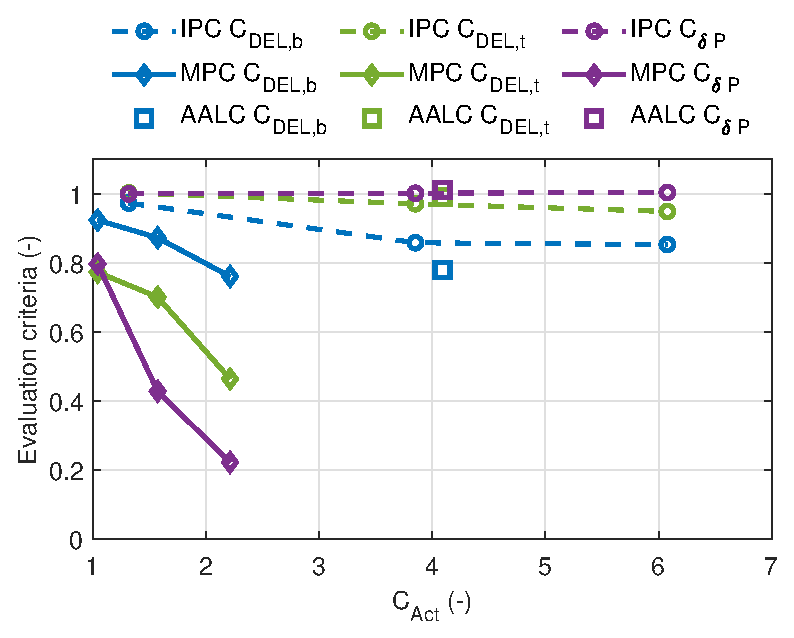
\includegraphics[width=0.65\textwidth]{figures/figures_WESC25/afig01_IPCMPCpareto.eps}
         
 
\caption[Evaluation criteria for qLMPC, IPC, and AALC for turbulent wind.] { Evaluation criteria for qLMPC, IPC, and AALC for turbulent wind (16\,m/s mean, IEC turbulence class B (14\%)). Criteria are tower base and blade DELs, power mean and standard deviation, and actuator power.}
         \label{fig:CtrlCompAll}
     \end{center}
 \end{figure}
 For qLMPC and IPC, three pitch rate limits were tested, resulting
 in different points along the actuator activity axis. Dashed lines with circles as markers show the result of IPC and solid lines with diamond markers the one obtained with qLMPC. The AALC optimization was run with a fixed pitch rate limit of 8\textdegree/s. Hence, only a single point, marked with a square, exists for AALC for each of the three criteria. As before, the blade and tower DEL lines are depicted in blue and green, respectively, and the power standard deviation in purple. The points with the smallest actuator criterion correspond to the numbers obtained with the rate limit of 4\textdegree/s and the ones with the largest to the values calculated for the rate limit of 13\textdegree/s.
 An important distinction between the three approaches is their effect on power variability.
 IPC and AALC only change $C_{\delta P}$ negligibly, with results at or marginally above unity, indicating that they
 preserve or very slightly increase power variance relative to the PI baseline. In contrast,
 qLMPC is the only controller that actively reduces power variance, with $C_{\delta P}$
 dropping to approximately 0.22 at the highest pitch rate limit. This is a direct consequence
 of the MIMO formulation of qLMPC, which simultaneously optimizes pitch and torque to
 minimize both structural loads and power fluctuations, whereas IPC and AALC operate as
 SISO pitch controllers without an explicit power smoothing objective.  The steep shape of the Pareto front $C_{\delta P}$ for qLMPC reflects that changes in the rotor and generator speed are penalized in the cost function. In Region III, where the turbine is operated around the rated generator torque and rated power, changes in power depend linearly on generator speed changes. As these are reduced considerably with the proposed qLMPC scheme, a smoother power yield is achieved.
 
 
 Tower DEL reductions, by contrast, are a byproduct of the more aggressive pitch actuation smoothing the aerodynamic thrust. The resulting fluctuations are the main source of tower fore-aft excitation and, to a lesser degree, of blade loads. As they are not directly included in the MPC cost function, their lines are flatter and do not show the curvature of a typical Pareto front.
 
All three controllers reduce blade and tower DELs relative to
 the PI baseline while maintaining the same mean power output. qLMPC consistently
 outperforms IPC across all three pitch rate settings, achieving lower DELs at comparable
 actuator activity. The AALC result at $C_\text{Act} \approx 4.2$ suggests that combining
 IPC with trailing edge flaps achieves blade DEL reductions comparable to qLMPC at lower
 pitch actuator demand, indicating that TEFs may offer a promising path to further blade
 load reduction without increasing pitch activity by an unacceptable factor.
 
 These results must be interpreted with caution, as the turbine and prediction models used
 in qLMPC are currently identical, which is unlikely to reflect real deployment conditions.
 Nevertheless, considerable improvements over baseline PI control are still expected, as
 reported in other MPC applications. The reliance of qLMPC on accurate wind preview
 information also presents a practical challenge.
 
 IPC, while delivering the least improvement of the three approaches, achieves reductions
 in the two-digit percentage range without requiring wind measurements or additional
 actuation hardware. AALC outperforms IPC by offloading part of the pitch actuation effort
 onto the trailing edge flaps, resulting in greater DEL reductions at lower pitch activity.
 These results highlight the trade-offs between controller complexity, sensor requirements,
 additional hardware such as TEFs, and load mitigation performance. The presented qLMPC offers
 the greatest potential for multi-objective control and is the only approach
 among the three that reduces power variability, but IPC remains a practical
 solution when lidar wind preview data is unavailable. 
 
 The presented qLMPC exploits that individual wind turbine dynamics are well understood and can be described in closed
 form as low-dimensional nonlinear ODEs. The following chapter discusses data-driven MPC for wind farms,
 where wake dynamics are time- and location-dependent and cannot be described by
 closed-form ODEs, yet must be accounted for in any MPC formulation.
 

 
 
 
    \chapter{Wind Farm Control} \label{sec:ApplicationtoWindFarmControl}

Wind turbines are grouped into farms to efficiently use locations suitable for wind energy harvesting. Within a wind farm, as many turbines as economically viable are installed, with their number limited by wake interactions. A higher turbine density per area reduces the cost of grid connection per turbine and lowers operation and maintenance costs. However, closely spaced turbines experience wake interactions, causing power losses due to reduced energy availability and increased mechanical loads on downstream turbines.
In \cite{houck2022review} wind farm control methods are surveyed, including Axial Induction Control (AIC), Wake Redirection Control (WRC), their combination, and active wake control. These methods have shown advantages in simulations of varying fidelity, and WRC has also demonstrated benefits in field tests. MPC schemes have been proposed in various studies, such as \cite{spudic2014distMPC_https://doi.org/10.1002/oca.2136, zhao2016coordinated, bay2018active, vali2019adjoint}. Unlike individual turbine dynamics, wake interactions in a wind farm cannot be accurately captured by low-order ODEs. Therefore, the approach applied to wind turbine control in Chapter~\ref{sec:Application to Wind Turbine Control4}, i.e., deriving nonlinear differential equations, creating a qLPV model, and using it for qLMPC control, is not applicable to wind farms. Nonetheless, MPC can be utilized by leveraging data-driven models. Recently, Koopman operator-based methods have proven successful \cite{castillo2020wind, cassamo2021model}. By applying Koopman lifting functions to open-loop simulation data and performing Dynamic Mode Decomposition (DMD), state-space models suitable for MPC algorithms can be obtained. AIC strategies have been developed to handle stationary \cite{sharan2022Koopman} and non-stationary inflow conditions \cite{dittmer2022data}, and a combined WRC-AIC scheme has shown potential for tracking high power demands \cite{dittmer2023koopman}.

Section \ref{sec:WindFarmSimulationWFSim} revisits the design of WFSim, the wind farm simulation tool used in this thesis, describing the modifications and enhancements necessary to model wind speed variations and to represent thrust and power output for turbines with intentional yaw misalignment. Section \ref{sec:AdaptiveWindFarmqLMPCforAIC} presents an adaptive AIC algorithm capable of handling changes in freestream wind speed. Section \ref{sec:WindFarmLinearMPCforWRC-AIC} first demonstrates wind farm power increases achieved with WRC, followed by a combined WRC-AIC algorithm for grid reference tracking under high power demands. The results of the adaptive AIC scheme have been published in \cite{dittmer2022data}, and those of the combined WRC-AIC algorithm in \cite{dittmer2023koopman}.

%Wind turbines are grouped into farms to efficiently use locations suitable for wind energy
% harvesting. Within a wind farm, as many turbines as economically viable are installed, with their
% number limited by wake interactions. A higher turbine density per area reduces the cost of grid
% connection per turbine and lowers operation and maintenance costs. However, closely spaced
% turbines experience wake interactions, causing power losses due to reduced energy availability and
% increased mechanical loads on downstream turbines. In \cite{houck2022review} wind farm control methods are surveyed, including Axial Induction Control (AIC), Wake Redirection Control (WRC), and Dynamic Induction Control (DIC). These
% methods have shown advantages in simulations of varying fidelity, and WRC has also
% demonstrated benefits in field tests. MPC schemes have been proposed in various studies,
% such as \cite{spudic2014distMPC_https://doi.org/10.1002/oca.2136, zhao2016coordinated, bay2018active, vali2019adjoint}. Unlike individual turbine dynamics, wake interactions in a wind farm cannot be accurately captured by low-order ODEs. Therefore, the approach applied to wind turbine control in
% Chapter~\ref{sec:Application to Wind Turbine Control4}, i.e., deriving nonlinear differential
% equations, creating a qLPV model, and using it for qLMPC control, is not applicable to wind farms.
% Nonetheless, MPC can be utilized by leveraging data-driven models. Recently, Koopman
% operator-based methods have proven successful \cite{castillo2020wind, cassamo2021model}. By
% applying Koopman lifting functions to open-loop simulation data and performing Dynamic Mode
% Decomposition (DMD), state-space models suitable for MPC algorithms can be obtained. AIC
% strategies have been developed to handle stationary \cite{sharan2022Koopman} and non-stationary
% inflow conditions \cite{dittmer2022data}, and a combined WRC-AIC scheme has shown potential for
% tracking high power demands \cite{dittmer2023koopman}.
% 
% Section \ref{sec:WindFarmSimulationWFSim} revisits the design of WFSim, the wind farm simulation
% tool used in this thesis, describing the modifications and enhancements necessary to model wind
% speed variations and to represent thrust and power output for turbines with intentional yaw
% misalignment. In its public release \cite{boersma2018control}, WFSim fixes the boundary conditions
% of the 2D wind field and uses constant thrust and power coefficients. Both restrictions are removed
% here: time-varying boundary conditions are introduced, without which an adaptive AIC algorithm
% cannot be demonstrated, and the actuator logic is extended by a lookup table reproducing the
% decrease of the power coefficient under yaw misalignment \cite{hulsman2022}, without which the
% power-loss trade-off inherent in wake redirection would not be represented. Section \ref{sec:AdaptiveWindFarmqLMPCforAIC} presents an adaptive AIC algorithm capable of
% handling changes in freestream wind speed. The underlying Koopman model predicts the effective
% wind speeds at both turbines from a single point wind measurement upstream of the first turbine
% together with the thrust control signals, i.e., from signals available on a real wind farm, without
% requiring knowledge of the flow field. Building on this model, the adaptive scheme updates the
% Koopman matrix only when past predictions and measurements diverge, and thereby maintains power
% reference tracking under changing inflow conditions and power demands. 
% Section \ref{sec:WindFarmLinearMPCforWRC-AIC} first demonstrates wind farm power increases
% achieved with WRC, followed by a combined WRC-AIC algorithm for grid reference tracking under high
% power demands. Treating the yaw angle as an active control input rather than an offline optimized
% parameter is shown to improve tracking of highly variable, high power references, both over AIC
% with a yaw angle pre-optimized using the Gaussian wake model of \cite{bastankhah2016experimental}
% and, more markedly, over baseline AIC at zero at zero yaw. The results of the adaptive AIC scheme have
%been published in \cite{dittmer2022data}, and those of the combined WRC-AIC algorithm in
%\cite{dittmer2023koopman}.

\section{Wind Farm Simulation with WFSim} \label{sec:WindFarmSimulationWFSim}
The wind farm simulation environment WFSim \cite{boersma2017tutorial} is employed both for generating open-loop data and for closed-loop controller testing. A short introduction to WFSim is provided in Section~\ref{sec:WakeModels}, which outlines the background on wind farm models and control. The 2D Navier–Stokes equations (NSE) are described in Section~\ref{Subsection:WindFarmSimulationModels}, and the actuator-disk turbine model is introduced in Section~\ref{Subsection:Windfarmcontrol}. WFSim allows the user to either choose from pre-existing layout definitions and sets of control signals, which may be used in open loop, or introduce new sets. A pre-existing layout of a two-turbine farm was selected, but several excitation signal sets were specifically designed for the studies on which this thesis is based as foundations for Koopman system identification. Similar to the easily interchangeable layout and control signal settings, the environment facilitates the integration of custom controller designs. While the flow and pressure calculations are utilized as intended, the applications in this thesis require significant modifications to the internal signal flow of the original MATLAB code.
In its publicly available release, WFSim does not allow variation in wind speed or direction, as the boundary conditions of the 2D wind field are fixed. To overcome this limitation, the code in \cite{dittmer2022data} is adapted to permit time-varying boundary conditions, a prerequisite for demonstrating an adaptive AIC algorithm. Similarly, modifications were introduced in \cite{dittmer2023koopman} to capture more realistic effects of intentional yaw misalignment within the WRC-AIC scheme. By default, the thrust and power coefficients in WFSim are constant. However, since the power coefficient in reality decreases with increasing yaw misalignment \cite{hulsman2022turbine}, the actuator logic was extended with a lookup table. This modification ensures that the controller accurately accounts for the power-loss trade-offs inherent in wake redirection. An overview of the modified program structure, followed by a discussion of the physical concepts represented in the implementation, is provided in the following section. Note that the latter is based on the spatio-temporal discretization and detailed derivation of the 2D NSE found in \cite{boersma2018control}.

\subsection{WFSim Program Structure and Code Modifications} \label{sec:WFSim Program Structure and Code Modifications}
Figure~\ref{fig:WFSimMesh2} illustrates the wind farm layout used for all studies described in this thesis, showing the positions of the two turbines within the simulated wind farm area.
\begin{figure}[htp]
    \centering
    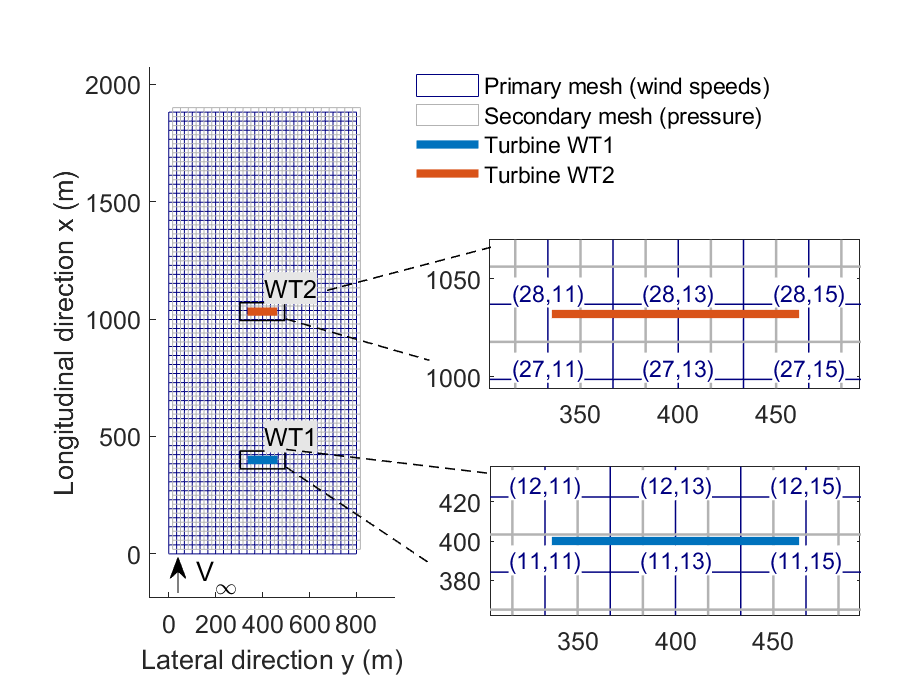
\includegraphics[width=0.65\textwidth]{figures/figures_IFAC23/gridmesh2_tex.eps}
    \caption[WFSim mesh setup for the two-turbine wind farm.]{WFSim mesh setup for the two-turbine wind farm. The primary mesh (blue) is used for wind speed calculations, and the secondary mesh (gray) for pressure. WT1 (upstream) and WT2 (downstream) are shown as blue and red bars, respectively. Zoomed-in areas show primary grid point indices.}
    \label{fig:WFSimMesh2}
\end{figure}
The simulation domain spans~1882\,m in the longitudinal direction and~800\,m in the lateral direction. The primary grid, in blue, is used to compute the longitudinal and lateral wind speeds, and the secondary grid, in gray, is utilized for pressure calculations. Both grids have identical dimensions with a total of 1250 nodes, consisting of 50 nodes in the longitudinal and 25 nodes in the lateral direction. This results in a spatial resolution of $\Delta x = 37.64\,\mathrm{m}$ and $\Delta y = 32\,\mathrm{m}$, with a 1:1 ratio between the primary and secondary grids. The grids are shifted so that the corner nodes of the secondary grid coincide with the center of the mesh cells of the primary grid. The upstream turbine WT1 is represented by a blue bar, and the downstream turbine WT2 by a red bar. The areas around the turbines are shown as zoomed-in plots to clarify which grid points are used in the calculation of the effective wind speeds. For WT1, these are five grid points located in the 11$^{\text{th}}$ row in the longitudinal direction, from the 11$^{\text{th}}$ to the 15$^{\text{th}}$ points in the lateral direction. For WT2, positioned downstream of WT1, the corresponding five points lie in the 27$^{\text{th}}$ longitudinal grid row. 

A considerable speed-up of the WFSim closed-loop simulation is achieved by reformulating the MPC objective function as a QP and avoiding unnecessarily re-initializing constant parameters in each call to the controller. This reformulation of the MPC algorithm results in a speed-up of the controller function execution by a factor of roughly 30 from 152.57\,s to 5.04\,s, and a reduction of the overall simulation time by a factor of nearly 7 from 177.2\,s to 26.2\,s, see Appendix~\ref{appendixC} for further details on the runtimes. Notably, the qLMPC algorithm achieves a mean execution time of 4.2\,ms per simulation step, rendering it potentially real-time capable, whereas the original NMPC requires a mean time of 127.14\,ms. The Koopman MPC algorithms discussed in this thesis are based on this QP formulation of the nonlinear MPC. 

Figure~\ref{fig:WFSimFlow}(a) presents the WFSim program structure diagram for a closed-loop simulation of the original nine-turbine setup. Figure~\ref{fig:WFSimFlow}(b) shows the function used for simulation of Koopman MPC schemes for the two-turbine setup presented in this thesis. While the general program flow and underlying NSE calculations of WFSim are preserved, considerable code modifications and enhancements are necessary in the initialization, the model and the MPC part of the code. These functions are highlighted in Figure~\ref{fig:WFSimFlow}(b) and functions introduced for the Koopman MPC are furthermore written in bold letters. The diagrams are generated using the MATLAB profiler during a closed-loop run with the nonlinear MPC controller integrated into WFSim and the Koopman MPC published in \cite{sharan2022Koopman}. The functions are reordered based on their dependencies to visualize the sequence of function calls.
%\begin{figure}[h]
%    \centering
%    \includegraphics[width=0.65\textwidth, trim=0mm 5mm 7mm 0.1mm, clip]{figuresBlockDiagram_IFAC23/FlowchartInitCtrlPlant_1.eps}
%    \caption{WFSim program structure diagram. Initialization, wind farm model, and controller functions are enclosed in black, blue, and red boxes, respectively. The modified functions \textit{Actuator} and \textit{BoundaryConditions} are highlighted in blue.}
%    \label{fig:WFSimFlow}
%\end{figure}
\begin{figure}[ht]
    \centering
    \subfloat[Original program structure]{
        \begin{minipage}[b]{0.495\textwidth}
            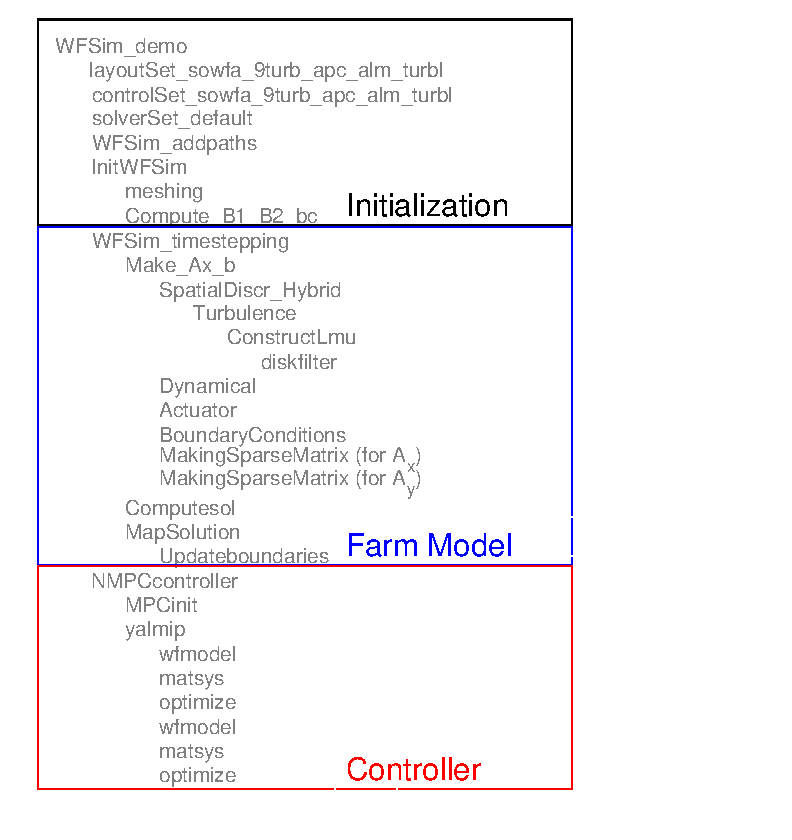
\includegraphics[width=\textwidth, trim=0mm 5mm 29.5mm 0.1mm, clip]{figures/figuresBlockDiagram_IFAC23/FlowchartInitCtrlPlant_1.eps}
        \end{minipage}
    } %\hfill 
    \subfloat[Modified program structure]{
        \begin{minipage}[b]{0.495\textwidth}
            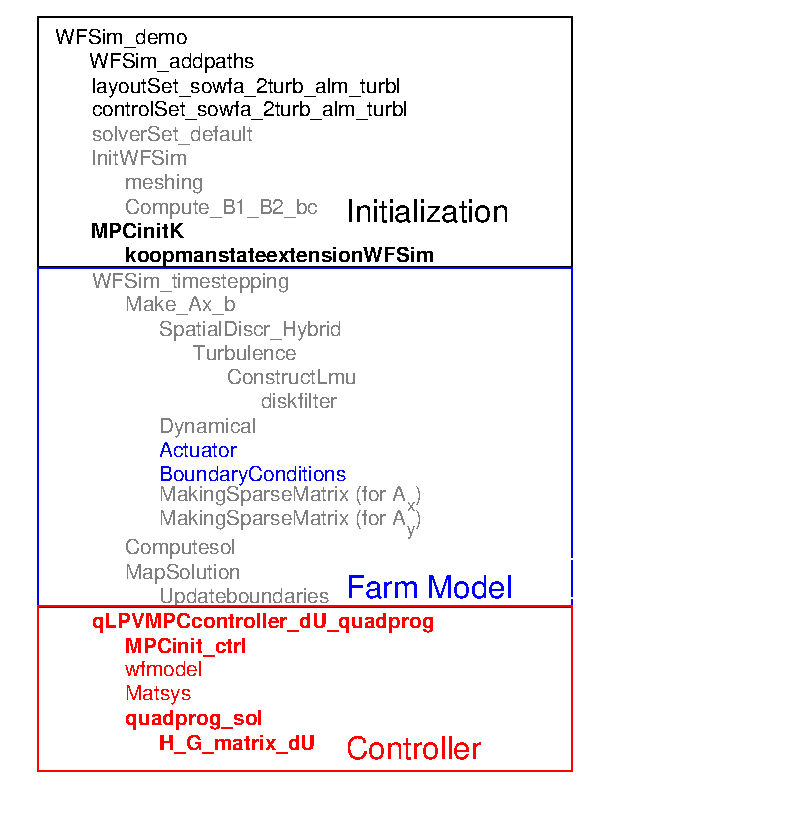
\includegraphics[width=\textwidth, trim=0mm 5mm 29.5mm 0.1mm, clip]{figures/figuresBlockDiagram_IFAC23/FlowchartInitCtrlPlant_2.eps}
        \end{minipage}
    }
    \caption[WFSim program structure diagram.]{WFSim program structure diagram. Initialization, wind farm model, and controller functions are enclosed in black, blue, and red boxes, respectively. Modified functions in (b) are highlighted in black, blue, and red within their respective sections, and functions added for Koopman MPC are indicated in bold.}
    \label{fig:WFSimFlow}
\end{figure}
The entry point to the simulation is the script \textit{WFSim\_demo.m}. Prior to the simulation loop, several initialization functions are called to define the environment and controller parameters as shown in Figure~\ref{fig:WFSimFlow}:

\begin{itemize}\item The script initializes the wind farm layout, setting the number of turbines and their positions, using functions with the naming pattern \textit{layoutSet\_sowfa\_...m}. It specifies the thrust and yaw control signals in \textit{controlSet\_sowfa\_...m}. For the open-loop data generation used to derive the Koopman models presented in \cite{sharan2022Koopman} and \cite{dittmer2022data}, custom signal sets are generated. On the other hand, for closed-loop studies, where only the initial control signal value is selected from the provided vectors and all consecutive control decisions are derived with the control algorithm, the existing files are selected for convenience.
    
    \item The simulation path is set via \textit{WFSim\_addpaths.m} and the solver settings are defined in \textit{solverSet\_default.m}. In the modified structure (Figure~\ref{fig:WFSimFlow}b), the path initialization is the first function to be called, as all commands handling the addition of functions to the executable MATLAB path are moved into this function for a cleaner program structure. It is also modified to ensure that all custom Koopman and QP-based functions can be executed.
    
    \item The function \textit{InitWFSim.m} initializes the wind field, while \textit{meshing.m} defines the computational grid and prepares the MATLAB structures for the simulation.
    
    \item The function \textit{Compute\_B1\_B2\_bc.m} computes the boundary conditions $\bm{b}^\mathrm{BC}$ and the associated matrices $B_1$ and $B_2$. The original implementation calls this function only once, resulting in static boundaries. The modified version calls it whenever the freestream wind changes, enabling non-stationary simulation runs \cite{dittmer2022data}.
    
    \item In the modified program flow, two new functions are added to the initialization phase: \textit{MPCinitK.m} and \textit{koopmanstateextensionWFSim.m}. These functions load the state space model containing the finite-dimensional representation of the Koopman operator, which are used for the subsequent MPC execution.
\end{itemize}
The changes to the turbine states, such as thrust and power, and the wind field at each mesh point are calculated within the simulation loop in \textit{WFSim\_timestepping.m}. The function \textit{Make\_Ax\_b.m} is the core of the WFSim simulation, assembling the system matrices through the following subfunctions:

\begin{itemize}\item In \textit{SpatialDiscr\_Hybrid.m}, a hybrid differencing scheme discretizes the convection terms of the NSE on the 2D mesh. It computes the convection coefficients in both the longitudinal and lateral directions, which are essential for solving the discretized fluid flow equations.
    
    \item The function \textit{Dynamical.m} adds the time-dependent terms of the NSE. It updates the discretization coefficients with unsteady contributions and builds the dynamic source terms representing mass and momentum storage effects based on the velocity field from the previous timestep.
    
    \item The function \textit{Actuator.m} models the actuator-disk representation of the wind turbines within the flow solver. It computes the thrust forces, wake deflection, and power extraction for each turbine. It inserts these forces into the momentum equations and updates turbine data, including power $P$, thrust $F_{T,r}$, yaw $\gamma$, and the coefficients $c_P$ and $c_F$. In \cite{dittmer2023koopman}, a lookup table is integrated into this function to dynamically adjust the power and thrust coefficients based on the yaw angle.
    
    \item In \textit{BoundaryConditions.m}, the boundary conditions for the discretized momentum equations are assigned, enforcing zero-gradient outflow and specific inflow conditions. As shown in the modified structure, this function is adapted in \cite{dittmer2022data} to account for a time-varying freestream wind.
    
    \item The function \textit{MakingSparseMatrix.m} creates the sparse matrix representation of the finite-volume discretization. It is called twice, once for the longitudinal and once for the lateral wind speed components, to construct the system matrices $A_x$ and $A_y$.
\end{itemize}
%
Following the matrix assembly, \textit{Computesol.m} solves the resulting system of equations to obtain the current wind speeds and pressure at the nodes as a vectorized solution. Finally, \textit{MapSolution.m} maps this vector back onto the 2D flow field and updates the boundary conditions for the subsequent simulation iteration.Figure~\ref{fig:WFSimFlow} illustrates the program structure diagram of the controller call within the red box, situated below the wind farm model functions (blue box). In the original code (Figure~\ref{fig:WFSimFlow}a), all controller information, including constant parameters, was re-initialized at every timestep using \textit{MPCinit.m}. In the versions developed in \cite{sharan2022Koopman}, \cite{dittmer2022data}, and \cite{dittmer2023koopman}, only the wind-dependent input matrices are updated, while all constant values are established during the initial setup. In the original implementation, the MATLAB-based modeling framework YALMIP \cite{lofberg2004yalmip} is then initialized to parse the optimization problem. The control signals, specifically the thrust and yaw commands, $C^{\prime}_T$ and $\gamma$, are calculated in the \textit{NMPCcontroller.m} function through three steps:

\begin{itemize}
    \item The individual system and input matrices for each turbine are computed in \textit{wfmodel.m}.
    \item In \textit{matsys.m}, these individual matrices are concatenated to form the global wind farm system and input matrices.
    \item The optimal control signals are obtained by solving the resulting MPC problem via \textit{optimize.m}.
\end{itemize}
%
In the modified structure (Figure~\ref{fig:WFSimFlow}b), this workflow is replaced by the \textit{qLPVMPCcontroller\_dU\_\allowbreak quadprog.m} function. This new controller utilizes matrices initialized in \textit{koopmanstateextensionWFSim.m} and initializes wind-dependent input matrices from \textit{MPCinit\_ctrl.m}. The functions \textit{wfmodel.m} and \textit{matsys.m} are modified to accommodate these changes and to construct the parameter-dependent Toeplitz-like matrices and boundary conditions for the QP formulation. These are passed to \textit{quadprog\_sol.m}, which calls the MATLAB solver \textit{quadprog.m}. While the original implementation performed two iterations to refine wind speed predictions, no clear benefit regarding tracking error minimization was observed in the studies forming the basis of this thesis when running the optimization twice. Consequently, the decision was made to calculate the farm control signal only once at each iteration. This further slightly streamlines the process, as less than 3\,ms are now used for each controller calculation. However, it should be noted that this reduction in complexity is secondary to the substantial computational gains achieved by the QP formulation itself.

The following section outlines the calculation of the wind field using the signals $C^{\prime}_T$ and $\gamma$ from \textit{Actuator.m}, the matrices $A_x$ and $A_y$ from \textit{MakingSparseMatrix.m}, and the boundary terms $B_1$, $B_2$, and $\bm{b}^\mathrm{BC}$ from \textit{Compute\_B1\_B2\_bc.m}.

\subsection{Physical Modeling Concepts in WFSim}
In WFSim, wake effects on air pressure and wind speed are modeled using the 2D NSE, which are defined in Equation~\eqref{eq:NSE2d} in Section~\ref{Subsection:WindFarmSimulationModels} and implemented in \textit{Make\_Ax\_b.m} and its subfunctions. For clarity, the NSE are restated here to directly link the physical concepts to their numerical implementation:  
\begin{align*} 
    \frac{\partial \bm{v}}{\partial t}+ (\bm{v}\cdot \nabla_H)\bm{v} + \nabla_H p + \nabla_H\cdot\bm{\tau}_h  - \bm{f} = \bm{0}_{2\times1},\quad  
    \nabla_H\cdot \bm{v} =  -\frac{\partial v_y}{\partial y}
\end{align*}
where $\bm{v} =[v_x\;\;v_y]^T$ consists of the wind components in the $x$- and $y$-directions, respectively. The horizontal gradient operator is $\nabla_H =[\partial/\partial x \;\; \partial/\partial y]^T$, and $p = p(x,y,z_h)$ is the normalized pressure at hub height $z_h$, scaled by air density $\rho_a$. The subgrid stress tensor for horizontal turbulence is denoted by $\bm{\tau}_h$, and $\bm{f}$ represents the turbine-induced forces acting on the flow. These terms are detailed in Section~\ref{Subsection:WindFarmSimulationModels}, which provides the physical background for the wind farm models.

The resulting two-dimensional aerodynamic force vector $\bm{f}_n$, which is applied to the flow field by turbine $n$, is calculated as:
\begin{align}\label{eq:forceNdim2}
    \bm{f}_n =  
    \begin{bmatrix}
        f_{x,n} \\
        f_{y,n}
    \end{bmatrix} 
    = \frac{1}{2} c_f C_{Tn}' \left(V_n \cos(\gamma_n)\right)^2
    \begin{bmatrix}
        \cos(\gamma_n + \phi) \\
        \sin(\gamma_n + \phi)
    \end{bmatrix} \in \mathbb{R}^{2\times 1},
\end{align}
where $C_{Tn}^{\prime}$ is the thrust control signal of turbine $n$ used to regulate axial induction. The variable $\gamma_n$ is the turbine yaw angle, and $\phi$ is the inflow wind direction. The scalar $V_n$ represents the magnitude of the effective wind speed at the rotor center of turbine $n$, and $c_f$ (kg/m) is a model calibration constant used to scale the applied thrust to match high-fidelity simulation or measurement data.

For the numerical implementation, the domain is discretized into an $n_p = n_x \cdot n_y$ grid of pressure cells. WFSim utilizes a staggered grid configuration: the longitudinal wind speed $v_x$ is stored on horizontal cell edges (normal to the vertical x-axis), and the lateral wind speed $v_y$ is stored on the vertical cell edges (normal to the horizontal y-axis). Note that in the WFSim matrix convention, the $x$-axis corresponds to the row index, i.e., the longitudinal direction, and the $y$-axis to the column index, the lateral direction.

This discretization yields $n_{v_x} = n_x \cdot (n_y+1)$ unknowns for the longitudinal velocity and $n_{v_y} = (n_x+1) \cdot n_y$ unknowns for the lateral velocity. Consequently, the 2D force components from Equation~\eqref{eq:forceNdim2} are mapped to the grid and assembled into the vector $\bm{f}$:
\begin{align}\label{eq:forceWFSim}
    \bm{f}_n \;\mapsto\; \bm{f} =
    \begin{bmatrix}
        \bm{f}_{x} \\[1mm]
        \bm{f}_{y}
    \end{bmatrix} \in \mathbb{R}^{(n_{v_x}+n_{v_y}) \times 1}, 
    \qquad 
    \bm{f}_{x} \in \mathbb{R}^{n_{v_x} \times 1}, \quad
    \bm{f}_{y} \in \mathbb{R}^{n_{v_y} \times 1}.
\end{align}
For the example utilized in this thesis, with $n_x = 50$ and $n_y = 25$, the dimensions are:
\begin{align*}
    n_{v_x} = 1300,\;  n_{v_y} = 1275, \;\text{and}\; n_{p} = 1250,
\end{align*}
which results in a total state dimension of $n_q = n_{v_x} + n_{v_y} + n_p = 3825$.

After spatial and temporal discretization, the system dynamics are described by the following differential equation:
\begin{align} \label{eq:WfsinGrid}
    E(q_k)q_{k+1} = Aq_k + \bm{b}(q_k, w_k)
\end{align}
where the system state vector $q_k \in \mathbb{R}^{\,n_q}$ contains the wind speed components and pressure at sample time $k$:
\[
q_k = 
\begin{bmatrix} 
    \bm{v}_x^T   & \bm{v}_y^T   & p^T   
\end{bmatrix}^T \in \mathbb{R}^{\,n_{q} \times 1}.
\]
The control input vector is defined as:
\[
w_k = 
\begin{bmatrix} 
    (\bm{C}_{T,k}^{\prime})^T   & \bm{\gamma}_k^T   
\end{bmatrix}^T   
\in \mathbb{R}^{\,2n_{\mathrm{WT}}\times 1},
\]
where $\bm{C}_{T,k}^{\prime}, \bm{\gamma}_k \in \mathbb{R}^{\,n_{\mathrm{WT}}}$ correspond to the thrust control signals and yaw angles of the $n_{\mathrm{WT}}$ turbines.

The matrices $E(q_k) \in \mathbb{R}^{\,n_{q} \times n_{q}}$ and $A \in \mathbb{R}^{\,n_{q} \times n_{q}}$ describe the interaction between the interior grid points, while $\bm{b}$ is the forcing vector combining boundary conditions and control inputs. Specifically, $E(q_k)$ and  $A$ are structured as
\begin{align} \label{eq:AGrid}
    E(q_k) =
    \begin{bmatrix}
        A_x(\bm{v_{x,k}},\bm{v_{y,k}}) & 0   & B_1 \\
        0   & A_y(\bm{v_{x,k}},\bm{v_{y,k}}) & B_2 \\
        B_1^T   & (2 B_2)^T   & 0
    \end{bmatrix} \text{ and } 
  A =
\begin{bmatrix}
    A_{11} & 0   & 0 \\
    0   & A_{22} &0 \\
    0   & 0   & 0
\end{bmatrix},
\end{align}
where $A_x \in \mathbb{R}^{\,n_{v_x} \times n_{v_x}}$ and $A_y \in \mathbb{R}^{\,n_{v_y} \times n_{v_y}}$ are the sparse discretization matrices for the longitudinal and lateral momentum equations.  The matrices $B_1 \in \mathbb{R}^{\,n_{v_x} \times n_p}$ and $B_2 \in \mathbb{R}^{\,n_{v_y} \times n_p}$ couple the pressure field to the momentum equations, while $B_1^T$ and $(2 B_2)^T$ represent the discrete continuity equation acting on the pressure term. The factor of 2 in the $(2B_2)^T$ term arises from a modeling heuristic used to approximate 3D flow effects within a 2D framework. By assuming the vertical flow divergence $\partial w / \partial z$ is approximately equal to the lateral divergence $\partial v / \partial y$, the continuity equation is modified to $\partial u / \partial x + 2\partial v / \partial y = 0$. This adaptation allows the model to simulate mass leakage into the third dimension, preventing the unphysical flow accelerations often seen in standard 2D wake models and providing a better fit to high-fidelity LES data. The diagonal blocks $A_{11} \in \mathbb{R}^{\,n_{v_x} \times n_{v_x}}$ and $A_{22} \in \mathbb{R}^{\,n_{v_y} \times n_{v_y}}$ describe the influence of the longitudinal and lateral velocities at the current time step on those in the next sample.

The forcing vector $\bm{b}(q_k, w_k) \in \mathbb{R}^{n_q\times 1}$ in Equation~\eqref{eq:WfsinGrid} is defined as:
\begin{align} \label{eq:bGrid}\bm{b}(q_k, w_k) =\begin{bmatrix}\bm{f}_x(q_k, w_k) + \bm{b}_x^\mathrm{BC} \\ \bm{f}_y(q_k, w_k) + \bm{b}_y^\mathrm{BC} \\ \bm{0}\end{bmatrix},\end{align}
where $\bm{f}_x$ and $\bm{f}_y$ are the discrete aerodynamic force contributions from the turbines—calculated via the actuator disk model—and $\bm{b}_x^\mathrm{BC}, \bm{b}_y^\mathrm{BC}$ represent the contributions from the velocity boundary conditions. The zero block corresponds to the continuity equation, which remains unforced as it represents the mass conservation constraint. Thus, $\bm{b}(q_k, w_k)$ encompasses all external inputs and boundary constraints driving the state evolution. Although the system state dimension $n_q$ is large, even for the two-turbine case, the matrices are highly sparse and structured due to the finite-volume discretization on the staggered grid. This sparsity allows Equation~\eqref{eq:WfsinGrid} to be solved efficiently using sparse linear algebra techniques.

In the following subsection, the specific wind farm layout and simulation parameters utilized for the studies in this thesis are detailed.
\subsection{WFSim Simulation Setup and Wind Farm Layout}
The simulation studies presented in this thesis, the adaptive AIC \cite{dittmer2022data} and the WRC-AIC \cite{dittmer2023koopman}, utilize an identical wind farm layout. This setup corresponds to the default two-turbine configuration in WFSim, which is also employed in the earlier study \cite{sharan2022Koopman}. The simulation parameters are summarized in Table~\ref{table:WfSim}. 
%
\begin{table}[ht]
    \centering
    \caption{WFSim simulation parameters for the two NREL 5MW turbine setup.}
    \label{table:WfSim}
    \begin{tabular}{l l l l} 
        \toprule
        Description & Symbol & Value & Unit\\
        \midrule
        Domain size &$L_x\times L_y$ & $1882\times 800$& $\text{m}^2$ \\
        Grid size  &$n_x\times n_y$ & $50\times 25$ & -\\
        Number of turbines& $n_{\text{WT}}$ & 2 & - \\
        Rotor diameter & $D$  & $126.4$& m \\
        Turbine spacing & $5D$ & 632 & m\\
        Sample time &$\Delta t$ & $1$ & s \\
        Longitudinal freestream wind &$v_{x,\infty}$&  $7 - 9$ & m/s \\
        Lateral freestream wind &$v_{y,\infty}$  & $0$ & m/s \\         
        Thrust controls & $C^{\prime}_{T,\text{min}}$, $C^{\prime}_{T,\text{max}}$ & 0.1, 2 & -\\
        Yaw angles &$\gamma_1$, $\gamma_2$ &  $0 - 25$, $0$ & deg\\
        \bottomrule
    \end{tabular}
\end{table}
%
The turbines are modeled after the NREL 5MW turbine, featuring a rotor diameter of $D = 126.4\,\text{m}$. They are spaced $632\,\text{m}$ apart, corresponding to a streamwise distance of five rotor diameters downstream ($5D$). The discrete simulation sample time is set to $1\,\text{s}$. Regarding wind conditions, the lateral freestream component is set to $0\,\text{m/s}$ for both studies. However, the longitudinal freestream wind speed $v_{x,\infty}$ differs: in the adaptive AIC study \cite{dittmer2022data}, it varies between $7\,\text{m/s}$ and $9\,\text{m/s}$, whereas in the WRC-AIC study \cite{dittmer2023koopman}, it is held constant at $8\,\text{m/s}$.

The thrust control inputs $C_T'$ are constrained within the range $[0.1, 2]$.  Both turbines face the wind directly ($\gamma = 0^{\circ}$) in the AIC algorithm. In the WRC-AIC application, the upstream turbine is permitted a maximum yaw misalignment of $25^{\circ}$.

With this simulation setup and the code modifications described in Section~\ref{sec:WFSim Program Structure and Code Modifications}, the adaptive qLMPC algorithm can be applied to the wind farm. The following section discusses the design and implementation of the AIC algorithm.

\section{Adaptive Wind Farm qLMPC with Thrust Control} \label{sec:AdaptiveWindFarmqLMPCforAIC}
Accurately describing the complex turbulence evolution caused by wakes using closed-form low-order ODEs is infeasible. Consequently, the standard MPC controller available in the open-source WFSim environment explicitly models only the turbine dynamics. Wake interactions are accounted for implicitly by utilizing the effective wind speeds at the turbines as inputs to the model. This architecture is illustrated in the block diagram in Figure~\ref{figBlockDiagramFarm}, presented in Section~\ref{Subsection:Windfarmcontrol}, which provides an overview of the WFSim MPC framework.

In this section, the data generation process for both open-loop training and closed-loop controller testing is described. This is followed by a discussion of the data handling procedures required to derive an Extended Dynamic Mode Decomposition (EDMD) model, along with a review of the resulting wind farm model and the MPC algorithm itself. Finally, simulation results for both open-loop wind estimation and closed-loop adaptive control are presented. These results demonstrate the capability of the adaptive algorithm to learn dynamics that were not present in the initial training data.

\subsection{Simulation Setup for Thrust Control}
Figure~\ref{fig:WFSimFlowAIC} visualizes the data flow of the qLMPC scheme for the two-turbine wind farm. The upstream turbine is denoted WT1 and the downstream turbine WT2. A key distinction from the original WFSim implementation is that the effective wind speeds of the turbines are not fed back directly to the controller. Instead, they are estimated using the EDMD-based model introduced in the previous work~\cite{sharan2022Koopman}. While the freestream wind speed was held constant in that study, in this work the longitudinal component $V_\infty = v_{x,\infty}$ is varied, while the lateral component $v_{y,\infty}$ remains zero.

\begin{figure}[htp]
    \centering
    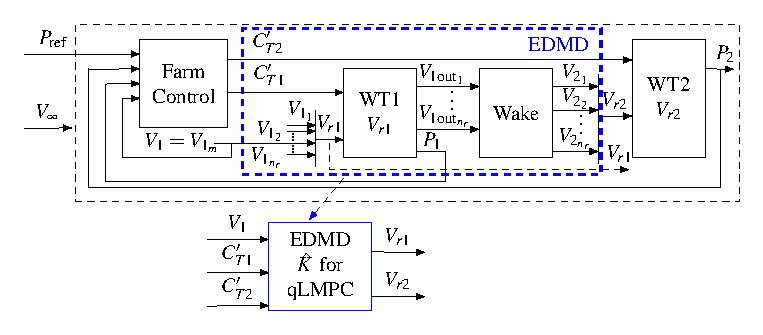
\includegraphics[width=1\textwidth,trim={0 0cm 0cm 0.3cm},clip]{figures/figuresBlockDiagram_IFAC23/farmCtrl16_P_multVthesis_EDMD.pdf}
    \caption[Block diagram of WFSim for AIC]{Block diagram of WFSim for AIC with farm control inputs $P_{\text{ref}}$, $P_1$, $P_2$, and $V_1 = V_{1_m}$, thrust control signals $C_{T1}^{\prime}$ and $C_{T2}^{\prime}$ and freestream wind $V_\infty$. Wind speeds directly in front and behind the turbine WT1 are $V_{1_1}$ to $V_{1_{n_r}}$ and $V_{1\text{out}_1}$ to $V_{1\text{out}_{n_r}}$. Wind speeds directly in front of the turbine WT2 are $V_{2_1}$ to $V_{2_{n_r}}$. The input to the EDMD model (dashed blue box in the closed-loop diagram and blue box below the diagram) are $V_1$, $C_{T1}^{\prime}$ and $C_{T2}^{\prime}$ and its output are the effective wind speeds $V_{r1}$ and $V_{r2}$.}
    \label{fig:WFSimFlowAIC}
\end{figure}

Given that the yaw angle of both turbines is fixed at $0^\circ$ for the AIC algorithm, the effective wind speed calculation, which is defined as the root mean square (RMS) of the wind speeds across the rotor, can be simplified relative to Equation~\eqref{eqEffWindSpdWT} by omitting the cosine term:
\begin{align} \label{eqEffWindSpdWTAIC}
    V_{ri} &=  \sqrt{\frac{1}{n_r} \sum_{j = 1}^{n_r} V_{i_j}^2},  
    \quad  V_{i_j} = v_{x,i_j},
\end{align}
where $v_{x,i_j}$ represents the wind speed component in the $x$-direction at the $j^{\text{th}}$ of $n_r$ mesh points in front of the $i^{\text{th}}$ turbine rotor.

The visualization in Figure~\ref{fig:WFSimFlowAIC} is adapted from the general WFSim diagram (Figure~\ref{figBlockDiagramFarm}) to explicitly distinguish between the local measured wind speed $V_{1_m}$ and the effective wind speed $V_{r1}$. To achieve this without overcrowding the diagram, the following modifications regarding signals and their visual representation as arrows are made:
\begin{itemize}
    \item In contrast to Figure~\ref{figBlockDiagramFarm}, where local wind speeds were summarized into vectors denoted $\bm{V}_{o1}$ and $\bm{V}_{o2}$, Figure~\ref{fig:WFSimFlowAIC} explicitly displays the individual wind speed signals $V_{1\text{out}_1}$ to $V_{1\text{out}_{n_r}}$ behind WT1. This visualization highlights the spatial signals involved in the wake interaction, while the corresponding signals behind WT2 are omitted, as they do not contribute to the MPC algorithm. Similarly to the rotor outflow, the rotor inflow velocities $V_{1_1}$ to $V_{1_{n_r}}$ and  $V_{2_1}$ to $V_{2_{n_r}}$ are visualized as arrows in Figure~\ref{fig:WFSimFlowAIC}.
    \item The turbine forces resulting from the effective wind speeds and control inputs are calculated within the standard WFSim MPC. However, since they are neither used in the cost function of that MPC scheme nor in the proposed scheme, they are omitted from Figure~\ref{fig:WFSimFlowAIC} to reduce visual clutter.
\end{itemize}
%
The signals depicted in Figure~\ref{fig:WFSimFlowAIC} are:
\begin{itemize}
    \item Freestream wind $V_\infty$: the freestream wind condition, consisting of a varying longitudinal component $v_{x,\infty}$ and a zero lateral component.
    \item Farm power reference $P_{\text{ref}}$: the reference power output for the entire wind farm.
    \item Measured wind $V_1$: the local wind speed at the rotor center of the upstream turbine (labeled $V_{1_m}$ in the figure).
    \item Rotor inflow $V_{1_1}$ to $V_{1_{n_r}}$: the array of local wind speeds at the $n_r$ grid points directly in front of the rotor of WT1.
    \item Effective wind $V_{r1}$: the RMS average of the inflow velocities $V_{1_1}$ to $V_{1_{n_r}}$ acting on WT1.
    \item Control signal $C_{T1}^{\prime}$: the thrust control signal applied to WT1.
    \item Power $P_1$: the electrical power generated by WT1.
    \item Rotor outflow $V_{1\text{out}_1}$ to $V_{1\text{out}_{n_r}}$: the local wind speeds at the grid points directly behind WT1.
    \item Rotor inflow $V_{2_1}$ to $V_{2_{n_r}}$: the array of local wind speeds directly in front of the rotor of WT2, which are affected by the wake of WT1.
    \item Effective wind $V_{r2}$: the RMS average of the inflow velocities $V_{2_1}$ to $V_{2_{n_r}}$ acting on WT2.
    \item Control $C_{T2}^{\prime}$: the thrust control signal applied to WT2.
    \item Power $P_2$: the electrical power generated by WT2.
\end{itemize}
Specific signals from this set are recorded during open-loop simulations to construct the linear EDMD models. The identified models utilize three inputs, the measured wind speed $V_1$ and the thrust control signals $C_{T1}^{\prime}$ and $C_{T2}^{\prime}$, to estimate two outputs, the effective wind speeds $V_{r1}$ and $V_{r2}$.

\subsection{Koopman-Based Identification of qLPV Models}
To derive a Koopman-based linear model for predicting the effective wind speeds, open-loop simulations are first performed to generate training data. Before applying EDMD, this data is lifted using nonlinear functions, following the fundamental principles of Koopman operator theory. This section summarizes the model identification procedure using EDMD and its adaptation for data-driven adaptive control. While the Koopman operator and its matrix representation are described in detail in Sections~\ref{KoopmanOperator} and~\ref{KoopmanIdentification}, key concepts are revisited here to establish the connection to the qLPV model utilized in the wind farm MPC algorithm.

\subsubsection{Koopman Matrix Creation}

Consider a linear system in the lifted space of the form:
\begin{align}
    \bm{\varphi}(k+1) &= \bm{A} \bm{\varphi}(k) + \bm{B} \bm{w}(k), 
    \quad \hat{\bm{x}}(k) = \bm{C} \bm{\varphi}(k), 
    \label{eq:linearPredictor}
\end{align}
where $\bm{\varphi} \in \mathbb{R}^{n_\varphi \times 1}$ is the lifted state vector containing $n_\varphi$ observables, and $\bm{w} \in \mathbb{R}^{n_w \times 1}$ denotes the input vector, which includes both control signals and measured disturbances. The vector $\hat{\bm{x}} \in \mathbb{R}^{n_x \times 1}$ represents the predicted output. The system dynamics are defined by the state matrix $\bm{A} \in \mathbb{R}^{n_\varphi \times n_\varphi}$, the input matrix $\bm{B} \in \mathbb{R}^{n_\varphi \times n_w}$, and the output matrix $\bm{C} \in \mathbb{R}^{n_x \times n_\varphi}$. The initial lifted state is given by $\bm{\varphi}(\bm{x}_0) = [g_{1}(\bm{x}_0)\;\; g_{2}(\bm{x}_0) \;\; \ldots\;\;g_{n_\varphi}(\bm{x}_0)]^T$.

In the proposed framework, the lifted state vector $\bm{\varphi}$ is structured such that its first $n_x$ elements correspond directly to the predicted output $\hat{\bm{x}}$, which are the effective wind speeds, followed by their quadratic and cubic terms:
\begin{align*}
    \bm{\varphi} &= [V_{r1} \quad V_{r2} \quad V^2_{r1} \quad V^2_{r2} \quad  V^3_{r1} \quad V^3_{r2}]^T   \in \mathbb{R}^{n_\varphi \times 1}, \\
    \hat{\bm{x}} &=  [V_{r1} \quad V_{r2}] ^T   \in \mathbb{R}^{n_x \times 1},
\end{align*}
with dimensions $n_\varphi = 6$ and $n_x = 2$. The input vector $\bm{w}$ contains the measured wind speed in front of the upstream turbine and the thrust control signals:
\begin{align*}
    \bm{w} = [V_1 \quad C^{\prime}_{T1} \quad C^{\prime}_{T2}]^T   \in \mathbb{R}^{n_w \times 1},
\end{align*}
with $n_w = 3$.

EDMD is employed to calculate the Koopman matrix, which approximates the infinite-dimensional Koopman operator $\mathcal{K}$ \cite{arbabi2018data}. To facilitate this, the extended lifted observables, which combine the nonlinear state observables and the inputs, are defined as:
\begin{align}\label{eq:extLiftObs}
    \bm{\tilde{\varphi}}(\bm{x},\bm{w}) = 
    \begin{bmatrix}
        \bm{g}(\bm{x}) \\ \bm{w}
    \end{bmatrix} \in \mathbb{R}^{(n_\varphi + n_w) \times 1}.
\end{align}
For the considered setup, this results in a total dimension of $n_\varphi + n_w = 9$. Here, $\bm{\varphi} = \bm{g}(\bm{x}) \in \mathbb{R}^{n_\varphi \times 1}$ denotes the vector of nonlinear state observables, and $\bm{w} \in \mathbb{R}^{n_w \times 1}$ is the input vector, which appears linearly in the lifted dynamics.

Given $n_o$ samples of state and input data collected in simulation runs, the data snapshot matrices are defined:
\begin{align} \label{eq:DataCollAIC}
    \bm{X} &= \bigl[ [\bm{x}(k)^T \quad \bm{w}(k)^T]^T \bigr]_{k=1}^{n_o-1} \in \mathbb{R}^{(n_x+n_w)\times (n_o-1)}, \\
    \bm{X}_{+} &= \bigl[ [\bm{x}(k+1)^T\quad \bm{w}(k+1)^T]^T \bigr]_{k=1}^{n_o-1} \in \mathbb{R}^{(n_x+n_w)\times (n_o-1)},
\end{align}
where the dimension of the combined state and input vector is $n_x + n_w = 5$. To ensure an accurate approximation of the system dynamics, the number of samples must be significantly larger than the dimension of the extended lifted space ($n_\varphi + n_w$). For the study presented here, a dataset of $n_o = 32987$ samples is utilized for identification.

The extended Koopman matrix $\tilde{\bm{K}}$ is obtained by solving the least-squares problem:
\begin{align}
    \min_{\tilde{\bm{K}}} \sum_{k=1}^{n_o-1} 
    \left\|  
    \begin{bmatrix} 
        \bm{g}(\bm{x}(k+1)) \\[1mm] 
        \bm{w}(k+1) 
    \end{bmatrix}   
    - \tilde{\bm{K}} 
    \begin{bmatrix} 
        \bm{g}(\bm{x}(k)) \\[1mm]
        \bm{w}(k) 
    \end{bmatrix} \right\|_2^2.
    \label{eq:ExtendedKoopmanMinimizationProblem}
\end{align}
This matrix possesses the block structure:
\begin{align}
    \tilde{\bm{K}} = \begin{bmatrix} 
        \bm{A}_{\hat{K}} & \bm{B}_{\hat{K}} \\ 
        \bm{A}_{w,\hat{K}} & \bm{B}_{w,\hat{K}} 
    \end{bmatrix},
\end{align}
where 
$\bm{A}_{\hat{K}} \in \mathbb{R}^{n_\varphi \times n_\varphi}$, 
$\bm{B}_{\hat{K}} \in \mathbb{R}^{n_\varphi \times n_w}$, 
$\bm{A}_{w,\hat{K}} \in \mathbb{R}^{n_w \times n_\varphi}$, 
and $\bm{B}_{w,\hat{K}} \in \mathbb{R}^{n_w \times n_w}$.

For controller design, only the system and input matrices $\bm{A}_{\hat{K}}$ and $\bm{B}_{\hat{K}}$ are required. Thus, problem~\eqref{eq:ExtendedKoopmanMinimizationProblem} simplifies to:
\begin{align}
    \min_{\bm{A}_{\hat{K}}, \bm{B}_{\hat{K}}} 
    \sum_{k=1}^{n_o-1} 
    \left\| \bm{g}(\bm{x}(k+1)) - \bm{A}_{\hat{K}} \bm{g}(\bm{x}(k)) - \bm{B}_{\hat{K}} \bm{w}(k) \right\|_2^2.
    \label{eq:ApproxKoopman}
\end{align}

With the data matrices defined as
\begin{align}\label{eq:G_Gplus_datamatrices}
    \bm{G} &= \bigl[ \bm{g}(\bm{x}(1)) \;\; \cdots \;\; \bm{g}(\bm{x}(n_o-1)) \bigr] \in \mathbb{R}^{n_\varphi \times (n_o-1)}, \\
    \bm{G}_{+} &= \bigl[ \bm{g}(\bm{x}(2)) \;\; \cdots \;\; \bm{g}(\bm{x}(n_o)) \bigr] \in \mathbb{R}^{n_\varphi \times (n_o-1)}, \\
    \bm{W} &= \bigl[ \bm{w}(1) \;\; \cdots \;\; \bm{w}(n_o-1) \bigr] \in \mathbb{R}^{n_w \times (n_o-1)},
\end{align}
the optimization problem can be equivalently rewritten in matrix form using the Frobenius norm:
\begin{align}
    \min_{\bm{A}_{\hat{K}}, \bm{B}_{\hat{K}}} 
    \left\| \bm{G}_{+} - \bm{A}_{\hat{K}} \bm{G} - \bm{B}_{\hat{K}} \bm{W} \right\|_F^2.
\end{align}
Defining the combined data matrix of lifted states and inputs as:
\begin{align}
    \bm{G}_w = \begin{bmatrix} \bm{G} \\ \bm{W} \end{bmatrix} \in \mathbb{R}^{(n_\varphi + n_w)\times (n_o-1)},
\end{align}
the analytical least-squares solution is given by:
\begin{align}\label{eq:Koop_G_Gplus_datamatrices}
    \hat{\bm{K}} = \begin{bmatrix} \bm{A}_{\hat{K}} & \bm{B}_{\hat{K}} \end{bmatrix} 
    = \bm{G}_{+}  \bm{G}_w^{\dagger}
    \in \mathbb{R}^{n_\varphi \times (n_\varphi + n_w)},
\end{align}
where ${}^\dagger$ denotes the Moore–Penrose pseudoinverse. Since the number of samples is significantly larger than the number of observables, i.e., $n_o \gg n_\varphi + n_w$, $\bm{G}_w$ has full row rank, and the pseudoinverse can be explicitly computed as:
\begin{align*}
    \bm{G}_w^{\dagger} = \bm{G}_w^T (\bm{G}_w \bm{G}_w^T)^{-1} \in \mathbb{R}^{(n_o-1) \times (n_\varphi + n_w)}.
\end{align*}
Substituting this into Equation~\eqref{eq:Koop_G_Gplus_datamatrices} confirms the dimensions:
\[
\underbrace{\hat{\bm{K}}}_{n_\varphi \times (n_\varphi + n_w)} = 
\underbrace{\bm{G}_{+}}_{n_\varphi \times (n_o-1)} \cdot 
\underbrace{\bm{G}_w^T}_{(n_o-1) \times (n_\varphi + n_w)} \cdot 
\underbrace{(\bm{G}_w \bm{G}_w^T)^{-1}}_{(n_\varphi + n_w) \times (n_\varphi + n_w)}.
\]
%
To utilize the identified matrix $\hat{\bm{K}}$ for linear model predictive control, it is partitioned into the system matrix $\bm{A}_{\hat{K}} \in \mathbb{R}^{n_\varphi \times n_\varphi}$ and the input matrix $\bm{B}_{\hat{K}} \in \mathbb{R}^{n_\varphi \times n_w}$. To account for the measured disturbance $V_1$ as an autonomous state within the prediction horizon, the input matrix is further split into $\bm{B}_d \in \mathbb{R}^{n_\varphi \times 1}$ for the disturbance and $\bm{B}_u \in \mathbb{R}^{n_\varphi \times (n_w-1)}$ for the control inputs $[C'_{T1} \;\; C'_{T2}]^T$. 

The final augmented Koopman matrix $\hat{\bm{K}}_{\text{aug}}$ is then constructed to include the disturbance dynamics. Assuming the disturbance remains constant over the prediction horizon, the augmentation is performed as follows:
\begin{align} \label{eq:AugmentedKoopmanMPC}
    \hat{\bm{K}}_{\text{aug}} = \left[\begin{array}{cc|c} 
        \bm{A}_{\hat{K}} & \bm{B}_d & \bm{B}_u\\ 
        \bm{0}_{1 \times n_\varphi} & 1 & \bm{0}_{1 \times (n_w-1)} 
    \end{array}\right] \in \mathbb{R}^{(n_\varphi+1) \times (n_\varphi+n_w)},
\end{align}
where the second row ensures the persistence of the measured wind speed disturbance throughout the prediction. This structure allows the MPC to treat the disturbance as a known, constant state during the optimization of the control sequence.

\subsubsection{Koopman Matrix Update}\label{subsec:koopmanOnlineUpdate}

The online update strategy employed here is based on the recursive least squares method proposed in \cite{cisneros2020data}. To minimize computational overhead and memory usage, the model is not updated continuously. Instead, an update is triggered only when the deviation between the measured outputs and the model predictions over a window of length $h$ exceeds a defined threshold $\nu$.

Let $\mathcal{X}_{\nu}$ denote the buffer containing the state and input vectors from the previous $h+1$ time instants:
\[
\mathcal{X}_{\nu} = \begin{bmatrix} x_{k-1}^T  & w_{k-1}^T  & \dots & x_{k-h-2}^T  & w_{k-h-2}^T  \end{bmatrix} \in \mathbb{R}^{1 \times (n_\varphi + n_w)(h+1)}.
\]
The triggering condition is formulated using the infinity norm, which allows the threshold $\nu$ to be interpreted in physical units independent of the window length $h$:
\begin{equation} \label{eq:add_data}
    \left\|
    \begin{bmatrix} 
        x_{k-h} \\ 
        x_{k-h+1} \\ 
        \vdots \\ 
        x_{k}
    \end{bmatrix}
    -
    \begin{bmatrix} 
        C\hat{K}\bm{\tilde{\varphi}}(z_{k-h-1}) \\[2mm] 
        C\hat{K}\bm{\tilde{\varphi}}\Big(
        \begin{bmatrix} 
            \hat{K}\bm{\tilde{\varphi}}(z_{k-h-1}) \\ 
            w_{k-h} 
        \end{bmatrix}
        \Big) \\[1mm] 
        \vdots \\[1mm]
        C\hat{K}\bm{\tilde{\varphi}}\Big(
        \begin{bmatrix}
            \hat{K}\bm{\tilde{\varphi}}\Big(
            \begin{bmatrix}
                \hat{K}\bm{\tilde{\varphi}}(\cdots) \\
                w_{k-2}
            \end{bmatrix}
            \Big) \\
            w_{k-1}
        \end{bmatrix}
        \Big)
    \end{bmatrix}
    \right\|_\infty \geq \nu,
\end{equation}
where the extended lifted observables $\bm{\tilde{\varphi}}$ are defined as in Equation~\eqref{eq:extLiftObs}, and $z_k = [x_k^T  \;\; w_k^T ]$ is a stacked vector selected from $\mathcal{X}_{\nu}$.

When this condition is met, the Koopman matrix is updated using data matrices $\mathbf{L}_u^+$ and $\mathbf{L}^+$. At initialization, $\mathbf{L}_u$ and $\mathbf{L}$ correspond to the correlation matrices derived from the original offline data matrices $\mathbf{G}_w$ and $\mathbf{G}_+$, see Equations~\eqref{eq:G_Gplus_datamatrices} to \eqref{eq:Koop_G_Gplus_datamatrices}. While \cite{cisneros2020data} utilizes only the current measurement, this work incorporates a batch of the last five measurement samples to provide low-pass filtering and reduced sensitivity noise. The batch data matrix is defined as:
\[
z_{k,5} = [z_{k-5} \;\; z_{k-4} \;\; \dots \;\; z_k]  \in \mathbb{R}^{ (n_x + n_w)\times 6}.
\]
The recursive updates are computed as a weighted sum of the existing correlation matrices $\mathbf{L}_u$ and $\mathbf{L}$ and the new data:
\begin{equation} \label{eq:GA_online}
    \begin{split}
        n_{\text{upd}}^+ &= n_{\text{upd}} + 1,\\
        \mathbf{L}_u^+ &= \frac{1}{n_{\text{upd}}^+} \Big( (n_{\text{upd}}^+-1)\mathbf{L}_u + \bm{\tilde{\varphi}}(z_{k,5}) \bm{\tilde{\varphi}}(z_{k,5})^T  \Big),\\
        \mathbf{L}^+ &= \frac{1}{n_{\text{upd}}^+} \Big( (n_{\text{upd}}^+-1)\mathbf{L} + \bm{\tilde{\varphi}}(z_{k,5}^+) \bm{\tilde{\varphi}}(z_{k,5})^T  \Big).
    \end{split}
\end{equation}
The counter $n_{\text{upd}}$ acts as a weighting factor. In \cite{cisneros2020data}, this counter monotonically increases. In contrast, the values $n_{\text{upd}}$ is reset to $1$ whenever the error norm falls below the threshold. This allows the model to adapt to changing dynamics rather than becoming rigid due to a large historical weight. Conversely, during active updates, the counter is incremented to integrate the new information.

Finally, accurate online identification requires sufficient spectral content in the input. Since standard control signals may not excite all dynamic modes, a low-amplitude band-limited white noise signal is superimposed on the control input during updates. %More details on the implementation of this excitation signal are provided in the results section.
%Future improvements may include explicit limits on $n_{\text{upd}}$ and the introduction of forgetting factors to balance recent and historical data, as suggested in \cite{zhang2019online}.
%Based on the theory in \cite{cisneros2020data}, a brief review on online update of koopman model is provided in this section. To avoid the memory management issues, we can only store $G$, $G_+$ and $U$ vectors at time $k$ ToDo: Make clear that Psi might be a matrix not a vector if more than one sample is included. Aso use our formulation  Phi*Phi' and X1 *Phi' where Phi= [x0;u0] 
% To do: Forgetting factors, weights between previous model and new data, 
% 'keep alert', find balance between new information
% add quotes (Zhang, Princeton, adaptive DMD) ,added several samples
% Differences to Pable: P initialized as 1, so offline identified model is used
% P is reset to 1 when no update is necessary (tuning knob -> future work to 
\subsection{qLMPC Design for Thrust Control}
The aim of wind farm control is good power reference tracking with minimal changes in control inputs, as discussed in, e.g., \cite{vali2019adjoint}, and our work on AIC proof of concept in WFSim, \cite{sharan2022Koopman, dittmer2022data}.

\subsubsection{Model Derivation and Cost Function}
As mentioned in Section~\ref{Subsection:Windfarmcontrol}, the main difference to the NMPC that ships with WFSim is that the effective wind speeds are estimated with a qLPV model. This has the advantage that for the first iteration of the MPC, the effective wind speeds are calculated using EDMD based on data acquired in open-loop WFSim simulations, thus adapting over the prediction horizon instead of being kept constant. Concretely, the model utilizes the wind speed in front of the first turbine $V_1$, the two thrust control signals $C_{T1}^{\prime}$ and $C_{T2}^{\prime}$, and the resulting effective wind speeds. Before applying EDMD, the data is modified with non-linear lifting functions, an idea inspired by Koopman theory, which applies the Koopman matrix as discussed in detail in Section~\ref{KoopmanIdentification}.

For the qLMPC design for adaptive AIC, the same discrete-time wind farm model is used as in the original WFSim NMPC algorithm described in Section~\ref{Subsection:Windfarmcontrol} in Equations~\ref{eqPowerWT} to~\ref{eqLinWF}. The procedure used to calculate the evolution of the wind farm power over a prediction horizon is repeated here for ease of understanding, with the only difference being that the yaw angle is fixed to zero. The state-space model of the $i^{\text{th}}$ turbine, assuming no yaw control or misalignment, is given by:
\begin{align} \label{eqPowerWTAIC_vector}
    \underbrace{
        \begin{bmatrix}
            P_i(k+1) \\[0.8mm]
            F_{T,ri}(k+1) \\[0.8mm]
            \hat{C}_{Ti}^\prime(k+1)
    \end{bmatrix}}_{\bm{x}_{\text{WT},i}(k+1) \in {\mathbb{R}}^{3\times 1}}
    &=
    \underbrace{(1-\tau)\,\bm{I}_{3\times3}}_{\bm{A}_{\text{WT},i} \in {\mathbb{R}}^{3\times 3}}
    \begin{bmatrix}
        P_i(k) \\[0.8mm]
        F_{T,ri}(k) \\[0.8mm]
        \hat{C}_{Ti}^\prime(k)
    \end{bmatrix}
    +
    \underbrace{\tau
        \begin{bmatrix}
            \tfrac{1}{2}\rho_a A_r V_{ri}^3 \\[0.8mm]
            \tfrac{1}{2}\rho_a A_r V_{ri}^2 \\[0.8mm]
            1
    \end{bmatrix}}_{\bm{B}_{\text{WT},i}(V_{ri}) \in {\mathbb{R}}^{3\times 1}} \, C_{Ti}^\prime(k),
\end{align}
where $k$ is the discrete sample time index and the constant $\tau$ is the discrete-time filter coefficient. The coefficient $\tau$ determines the weighting between the current state and the new input at each time step, thereby controlling the response speed of the turbine states. The state vector is defined as
\begin{align*}
    \bm{x}_{\text{WT},i} = [P_i \quad F_{T,ri} \quad \hat{C}_{Ti}^\prime]^T,
\end{align*}
where $P_i$ is the power, $F_{T,ri}$ is the thrust force of the $i^{\text{th}}$ turbine, and $\hat{C}_{Ti}^\prime$ is the filtered thrust control signal. 

The individual turbine models are concatenated into a qLPV system with the vector of all effective wind speeds $\bm{V}_r$ as the scheduling parameter vector:
\begin{align} \label{eqLinWFAIC}
    \bm{x}_{\text{WF}}(k+1) &= \bm{A}_{\text{WF}} \bm{x}_{\text{WF}}(k) + \bm{B}_{\text{WF}}(\bm{V}_r) \, \bm{C}_{T}^\prime(k),\\
    P_{\text{WF}}(k) & = \underbrace{\bm{1}_{1 \times n_{\text{WT}} } \otimes [1 \quad 0 \quad 0]}_{\bm{C}_{\text{WF}} \in {\mathbb{R}}^{1 \times 3n_\text{WT}}} \, \bm{x}_{\text{WF}}(k), \label{eqLinWFAIC2}
\end{align}
where $\bm{A}_{\text{WF}} \in {\mathbb{R}}^{3n_\text{WT} \times 3n_\text{WT}}$ is a block-diagonal matrix and $\bm{B}_{\text{WF}}(\bm{V}_r) \in {\mathbb{R}}^{3n_\text{WT} \times n_\text{WT}}$ is a vertical concatenation of the turbine input matrices. The wind farm power $P_{\text{WF}}$ is the sum of all individual turbine powers, $P_{\text{WF}} = \sum_{i=1}^{n_{\text{WT}}} P_i$.

The farm-level state and input vectors are defined as:
\begin{align*}
    \bm{x}_{\text{WF}} &= [\bm{x}_{\text{WT}1}^T \quad \bm{x}_{\text{WT}2}^T \quad \dots \quad \bm{x}_{\text{WT} n_{\text{WT}}}^T ]^T \in {\mathbb{R}}^{3n_\text{WT}},\\
    \bm{C}_{T}^\prime &= [C_{T1}^\prime \quad C_{T2}^\prime \quad \dots \quad C_{T n_{\text{WT}}}^\prime ]^T \in {\mathbb{R}}^{n_\text{WT}},\\
    \bm{V}_r &= [V_{r1} \quad V_{r2} \quad \dots \quad V_{r n_\text{WT}}]^T \in {\mathbb{R}}^{n_\text{WT}}.
\end{align*}
These vectors are used in combination with the parameter-dependent Toeplitz-like matrices built from $\bm{A}_{\text{WF}}$, $\bm{B}_{\text{WF}}$, and  $\bm{C}_{\text{WF}}$ to predict the farm power trajectory similarly to the approach discussed in Section~\ref{sec:qLMPCOptimizationAlgo} and Equation~\eqref{eq:nearlyToeplitzMat}.

The cost function $J(\bm{U})$ is formulated to minimize the tracking error $\bm{E}$ and control increments $\Delta \bm{U}$:
\begin{align} \label{eq:NMPCcostAIC}
    J(\bm{U}) = \underbrace{\bm{E}^T Q \bm{E}}_{J_Q (\bm{U})} + \underbrace{\Delta \bm{U}^T R \Delta \bm{U} }_{J_R ( \bm{U})},
\end{align}
with weighting matrices $Q = q \cdot \bm{I}_{n_h \times n_h}$ and $R = r \cdot \bm{I}_{n_{hu}\times n_{hu}}$. The tracking error trajectory $\bm{E}(k)$ is defined as:
\begin{equation}\label{eq:errortraject}
    \begin{aligned}
        \bm{E}(k) &= P_{\text{ref}}(k) \cdot \bm{1}_{n_h \times 1} - \bm{P}_{\text{WF}}(k) \\
        &= [ e(k) \quad e(k+1) \quad \dots \quad e(k + n_h-1) ]^T \in \mathbb{R}^{n_h \times 1},
    \end{aligned}
\end{equation}
where $e = P_{\text{ref}} - P_{\text{WF}}$. Assuming a constant power reference over the horizon, we define $\bm{P}_{\text{ref}} = P_{\text{ref}} \cdot \bm{1}_{n_h \times 1}$. The predicted power and control trajectories are given by:
\begin{equation} \label{eq:UandDUAIC} 
    \begin{aligned} 
        \bm{P}_{\text{WF}}(k) &= [ P_{\text{WF}}(k) \quad \dots \quad P_{\text{WF}}(k + n_h-1)]^T, \\
        \bm{U}(k) &= [ U^T (k) \quad \dots \quad U^T (k+n_h-1) ]^T \in \mathbb{R}^{n_{hu}\times 1}, \\
        \Delta \bm{U}(k) &= [ (U(k) - U(k-1))^T \quad \dots \quad (U(k+n_h-1) - U(k+n_h-2))^T ]^T,
    \end{aligned} 
\end{equation}
where $U = [C_{T1}^\prime \quad \dots \quad C_{Tn_{\text{WT}}}^\prime]^T$. For the two-turbine case with $n_h = 10$, this yields $\bm{E} \in \mathbb{R}^{10\times 1}$ and $\bm{U}, \Delta \bm{U} \in \mathbb{R}^{20\times 1}$.

Finally, the constrained optimization problem is stated as:
\begin{align} \label{eq:ObjFunAIC}
    \begin{array}{l} 
        \underset{\bm{U}(k)}{\text{minimize }} J(\bm{U}(k)) = \bm{E}(k)^T Q \bm{E}(k) + \Delta \bm{U}(k)^T R \Delta \bm{U}(k) \\
        \text{subject to }\\
        \bm{x}_{\text{WF}}(k+j+1) = \bm{A}_{\text{WF}} \bm{x}_{\text{WF}}(k+j) + \bm{B}_{\text{WF}}(\bm{V}_r) \bm{C}_{T}^\prime(k+j) \\
        P_{\text{WF}}(k+j) = \bm{C}_{\text{WF}} \bm{x}_{\text{WF}}(k+j), \quad j = 0, \dots, n_h-1.
    \end{array}
\end{align}

\subsubsection{QP Formulation and Gradient Derivation}
Note that, unlike the velocity-based wind turbine qLMPC described in Equation~\eqref{eq:ObjFunWT}, the optimization parameters are the elements of the control vector trajectory $\bm{U}$, and not their differences over time, i.e., $\Delta \bm{U}$. Consequently, the penalty term on the control input, $J_R$, must be reformulated to depend on the trajectory $\bm{U}$ rather than the differences $\Delta \bm{U}$.

Directly substituting the linear model into the terms of the tracking error and input trajectories yields
\begin{equation} \label{eq:cost_termsAIC} \begin{aligned} J_Q(\bm{U}(k)) &= \big(\bm{P}_{\text{ref}}(k) - (\tilde{L} \bm{x}_{\text{WF}}(k) + \tilde{S} \bm{U}(k))\big)^T  Q \big(\bm{P}_{\text{ref}}(k) - (\tilde{L} \bm{x}_{\text{WF}}(k) + \tilde{S} \bm{U}(k))\big), \\[1ex] J_R(\bm{U}(k)) &= \big(\mathcal{D} \bm{U}(k) + \mathcal{C} U(k-1)\big)^T  R \big(\mathcal{D} \bm{U}(k) + \mathcal{C} U(k-1)\big), \end{aligned} 
\end{equation}
with the matrices $\mathcal{D}$ and $\mathcal{C}$ providing the linear relation $\Delta \bm{U}(k) = \bm{\mathcal{D}} \bm{U}(k) + \bm{\mathcal{C}} U(k-1)$. The current state vector $\bm{x}_{\text{WF}}(k)$, which is used to initialize the trajectory, is calculated from the state and input at the previous sample time $k-1$. The optimal control input trajectory $\bm{U}(k)$ is found by solving a QP algorithm, similar to the one used for individual wind turbines.
%

The matrices $\tilde{L} \in \mathbb{R}^{n_h \times 3n_{\text{WT}}}$ and $\tilde{S} \in \mathbb{R}^{n_h \times n_{hu}}$ calculate the predicted power trajectory $\bm{P}_{\text{WF}}(k) = [P_{\text{WF}}(k+1), \dots, P_{\text{WF}}(k+n_h)]^T$ based on the state-space model:
\begin{equation} \label{eq:ltildeWF}
    \begin{aligned} 
        \tilde{L} &= 
        \begin{bmatrix} 
            C_{\text{WF}} A_{\text{WF}} \\ C_{\text{WF}} A_{\text{WF}}^2 \\ \vdots \\ C_{\text{WF}} A_{\text{WF}}^{n_h} 
        \end{bmatrix}, \quad 
        \tilde{S}(\bm{V}_r) &= 
        \begin{bmatrix} 
            C_{\text{WF}} B_{\text{WF}}(\bm{V}_r) & 0 & \cdots & 0 \\ 
            C_{\text{WF}} A_{\text{WF}} B_{\text{WF}} (\bm{V}_r)  & C_{\text{WF}} B_{\text{WF}}(\bm{V}_r)  & \cdots & 0 \\ 
            \vdots & \vdots & \ddots & \vdots \\ 
            C_{\text{WF}} A_{\text{WF}}^{n_h-1} B_{\text{WF}}(\bm{V}_r)  & C_{\text{WF}} A_{\text{WF}}^{n_h-2} B_{\text{WF}} (\bm{V}_r) & \cdots & C_{\text{WF}} B_{\text{WF}} (\bm{V}_r) 
        \end{bmatrix}.
    \end{aligned}
\end{equation}
The matrices $\bm{\mathcal{D}}$ and $\bm{\mathcal{C}}$ can be written in terms of the optimization variable $\bm{U}(k)$:
\begin{align*}
    \bm{\mathcal{D}} &= \bm{I}_{n_{hu} \times n_{hu}} - 
    \begin{bmatrix}
        \bm{0}_{n_u \times n_u(n_h-1)} & \bm{0}_{n_u \times n_u} \\ 
        \bm{I}_{n_u(n_h-1) \times n_u(n_h-1)} & \bm{0}_{n_u(n_h-1) \times n_u}
    \end{bmatrix}, \\
    \bm{\mathcal{C}} &= -\begin{bmatrix} \bm{I}_{n_u \times n_u} \\ \bm{0}_{n_u(n_h-1) \times n_u} \end{bmatrix}.
\end{align*} 
This block-shift structure ensures that each control increment is calculated as the difference between a turbine's current input and its input at the previous time step. For a wind farm with $n_u = 2$ and a horizon $n_h = 10$, the matrices $\bm{\mathcal{D}} \in \mathbb{R}^{20 \times 20}$ and $\bm{\mathcal{C}} \in \mathbb{R}^{20 \times 2}$ are defined as:
\begin{align*}
    \bm{\mathcal{D}} &= \begin{bmatrix} 
        1 & 0 & 0 & 0 & \cdots & 0 \\
        0 & 1 & 0 & 0 & \cdots & 0 \\
        -1 & 0 & 1 & 0 & \cdots & 0 \\
        0 & -1 & 0 & 1 & \cdots & 0 \\
        \vdots & \vdots & \ddots & \ddots & \ddots & \vdots \\
        0 & 0 & \cdots & -1 & 0 & 1
    \end{bmatrix}, \quad
    \bm{\mathcal{C}} = \begin{bmatrix} 
        -1 & 0 \\
        0 & -1 \\
        0 & 0 \\
        0 & 0 \\
        \vdots & \vdots \\
        0 & 0
    \end{bmatrix}.
\end{align*}
%In this structure, $\bm{\mathcal{D}}$ is an identity matrix with a negative identity block $\bm{-I}_{2 \times 2}$ starting at the $(3,1)$ position. This ensures that the difference is taken between the same turbine's control input at consecutive time steps.
%
In addition to the filtered matrices $\tilde{L}$ and $\tilde{S}(V_r)$, corresponding unfiltered matrices $L \in \mathbb{R}^{3n_h n_{\text{WT}} \times 3n_{\text{WT}}}$ and $S(V_r) \in \mathbb{R}^{3n_h n_{\text{WT}} \times n_{hu}}$ are defined. These matrices map the current state $\bm{x}_{\text{WF}}(k)$ and the control input trajectory $\bm{U}(k)$ to the predicted state trajectory over the horizon:
\begin{align*}
    \bm{X}_{\text{WF}}(k +1) = \begin{bmatrix} \bm{x}_{\text{WF}}(k+1) \\ \vdots \\ \bm{x}_{\text{WF}}(k+n_h) \end{bmatrix} = L \bm{x}_{\text{WF}}(k) + S(V_r) \bm{U}(k) \in \mathbb{R}^{3 n_h n_{\text{WT}} \times 1}.
\end{align*}
The unfiltered matrices are utilized for predicting the evolution of the effective wind speeds. Specifically, the future effective wind speeds are estimated via the filtered thrust control inputs, which are extracted from the predicted state trajectory $\bm{X}_{\text{WF}}$.

The cost function from Equation~\eqref{eq:ObjFunAIC} is reformulated as a sequence of quadratic sub-problems, following the approach in \cite{gonzalez2020nonlinear}. For a cost $J(\bm{U})$ subject to constraints $g(\bm{U}) \leq 0$, the quadratic sub-problem at the $l$-th iteration is:
\begin{equation} \label{eq:ObjFunAICapprox}
    \begin{aligned} 
        \underset{ \tilde{\bm{U}}} {\text{minimize}} \quad & \frac{1}{2}\tilde{\bm{U}}^T \nabla^2 J(\bm{U}^l) \tilde{\bm{U}} + \nabla J(\bm{U}^l)^T \tilde{\bm{U}} \\
        \text{subject to} \quad & \nabla g(\bm{U}^l) \tilde{\bm{U}} + g(\bm{U}^l) \leq 0,
    \end{aligned}
\end{equation}
where $\bm{U}^l$ is the current estimate and $\tilde{\bm{U}} = \bm{U} - \bm{U}^l$ is the optimization variable. The gradients of the cost terms are:
\begin{align*} 
    \nabla J_Q (\bm{U}) &= 2 \tilde{S}^T Q \left( (\tilde{L} \bm{x}_{\text{WF}}(k) + \tilde{S} \bm{U}^l) - \bm{P}_{\text{ref}}(k+1) \right), \\
    \nabla J_R(\bm{U}) &= 2 \bm{\mathcal{D}}^T R (\bm{\mathcal{D}} \bm{U}^l + \bm{\mathcal{C}} U(k-1)),
\end{align*} 
and the corresponding Hessians are constant:
\begin{equation*} 
    \nabla^2 J_Q = 2 \tilde{S}^T Q \tilde{S}, \quad \nabla^2 J_R = 2 \bm{\mathcal{D}}^T R \bm{\mathcal{D}}.
\end{equation*} 

The control trajectory is subject to the constraints $\bm{U}_{\min} \leq \bm{U} \leq \bm{U}_{\max}$, where $\bm{U}_{\min}$ and $\bm{U}_{\max}$ are vectors containing the limits $u_{\min} = 0.1$ and $u_{\max} = 2$ from Table~\ref{table:WfSim}. In standard QP form, these are expressed as $A_{\text{const}} \bm{U} \leq b_{\text{const}}$, with:
\[
A_{\text{const}} = \begin{bmatrix} I \\ -I \end{bmatrix}, \qquad b_{\text{const}} = \begin{bmatrix} \bm{U}_{\max} \\ -\bm{U}_{\min} \end{bmatrix}.
\]
For the sub-problem in $\tilde{\bm{U}}$, the constraints are shifted relative to the current estimate $\bm{U}^l$:
\[
A_{\text{const}} \tilde{\bm{U}} \le \underbrace{b_{\text{const}} - A_{\text{const}} \bm{U}^l}_{\bm{b}_{\text{shifted}}}.
\]%\[
%\bm{U}_{\min} \le \bm{U}_\ell \le \bm{U}_{\max},
%\]
%otherwise the QP problem will be infeasible.
The implementation of the controller is summarized in Algorithm~\ref{algo:qLPVMPCAIC}. 
\begin{algorithm} \caption{Adaptive qLMPC for AIC}\label{algo:qLPVMPCAIC}
    \begin{algorithmic}[1]
        \Procedure{qLMPC\_AIC}{$P_{\text{ref}}, V_1 (k), \bm{x}_{\text{WF}}(k), \bm{u}(k-1), \mathcal{X}_{\nu}$}
        \State Initialize farm model, weight matrices $\bm{Q}, \bm{R}$, and horizon $n_h$
        \State Initialize data matrices $\mathbf{L}_u$ and $\mathbf{L}_+$ from \eqref{eq:G_Gplus_datamatrices}
        \State $k \gets 0$
        \While{$k < T_{\text{end}}$}
        \State \textbf{Adaptive Model Update:}
        \If{$k > h$ \textbf{and} criterion \eqref{eq:add_data} exceeds $\nu$ using buffer $\mathcal{X}_{\nu}$}
        \State Update $\mathbf{L}_+$ and $\mathbf{L}_u$ with new data from $\mathcal{X}_{\nu}$
        \State $\hat{\bm{K}} \gets \mathbf{L}_+ (\mathbf{L}_u)^\dagger$ \Comment{Recalculate Koopman operator}
        \EndIf
        \State $l \gets 0$
        \While{stop criterion not met} \Comment{Successive QP iterations}
        \State Estimate $\bm{V}_r$ trajectory using $\hat{\bm{K}}$, $V_1(k)$, and $\bm{x}_{\text{WF}}(k)$
        \State Compute batch matrices $L, S, \tilde{L}, \tilde{S}$ based on estimated $\bm{V}_r$
        \State Solve QP \eqref{eq:ObjFunAICapprox} to obtain optimal trajectory $\bm{U}^l(k)$
        \State Predict $\bm{X}_{\text{WF}}^{l}(k+1) = L \bm{x}_{\text{WF}}(k) + S \bm{U}^l(k)$
        \State $l \gets l + 1$
        \EndWhile
        \State Apply first control $\bm{u}(k)$ from $\bm{U}^l(k)$ to the system
        \State \textbf{Update Buffer:}
        \State $\mathcal{X}_{\nu} \gets$ update with $\{\bm{x}_{\text{WF}}(k), \bm{u}(k)\}$ and slide window
        \State $k \gets k + 1$
        \EndWhile
        \EndProcedure
    \end{algorithmic}
\end{algorithm}

The primary distinction between this approach and the individual turbine control in Algorithm~\ref{algo:qLPVMPC} is the integration of the data-driven wind speed predictor. The Koopman-based model is updated online whenever the discrepancy between historical predictions and the actual states, defined by the criterion in \eqref{eq:add_data}, exceeds the threshold $\nu$.

At each sample time $k$, the controller requires a set of external signals and internally stored variables to compute the optimal control sequence:
\begin{enumerate}
    \item The reference power trajectory $\bm{P}_{\text{ref}}(k)$ and the current measured wind speed $V_{1}(k)$ at the upstream turbine must be provided.
    \item The algorithm utilizes the current state vector $\bm{x}_{\text{WF}}(k)$ and the previous control $\bm{u}(k-1)$. Additionally, it maintains the buffer $\mathcal{X}_{\nu}$ containing the most recent $h+1$ state-input pairs, which are mapped through the extended lifting $\bm{\tilde{\varphi}}$ to evaluate the discrepancy criterion in \eqref{eq:add_data}.
\end{enumerate}


%
% &= 2R [(\Delta U_1 - \Delta U_2),(\Delta U_3 - \Delta U_2),..., \Delta U_N]^T  
%  \nabla J(\bm{U}_l)&= 2 (\tilde{S} ^T   Q (\lambda \zeta_{d,k}+\tilde{S} \bm{U}_l - \bm{P}_{ref}) + \mathcal{D}^T   R (\mathcal{D}\bm{U}_l + \mathcal{C}) + R_{\gamma} \bm{U}_l) \text{ and }  H J_Q(\bm{U}_l) = 2(S^T  QS+\mathcal{D}^T  R\mathcal{D} + R_\gamma).


%\label{eq:Koop_G_Gplus_datamatrices}
%\hat{\bm{K}} = \begin{bmatrix} \bm{A}_{\hat{K}} & \bm{B}_{\hat{K}}   
    %$\mathbf{L}_u$ and $\mathbf{L}_+$ correspond to the original data matrices $\mathbf{G}_w$ and $\mathbf{G}_+$ introduced in Equations~\eqref{eq:G_Gplus_datamatrices} to~\eqref{eq:Koop_G_Gplus_datamatrices}.
    %Therefore, the matrices of the quadratic sub-problem constraints are \\
    %\begin{align*} \label{eqn:constraint}
    %    A_{const} = [I_{N\cdot n_T },- I_{N\cdot n_T }]^T  , \quad
    %    b_{const} = [-u_M \mathbf{1}^{1\times N\cdot n_T}, u_m \mathbf{1}^{1\times N\cdot n_T}]^T  
    %     \end{align*}
%In the EIODMD approach based on $\hat{K}_2$ the power $P_{\text{WF}}$ is estimated directly. The result is a linear MPC as this omits the effective wind speeds as scheduling parameters. For this second control algorithm, the stacked Toeplitz matrices $\Lambda_{K}$ and $S_{K}$ are based on the matrices $A_{K}$, $B_{K}$, $C_{K}$ and $D_{K}$ as
% {\scriptsize
    %}
%For EIODMD $P_{\text{WF}}$ is estimated directly, so there is $\tilde{L}_{K} = \Lambda_{K}$ and $\tilde{S}_{K} = S_{K}$.\\
%
\subsection{Results} \label{section:AICWindFarmControl}
The qLMPC described in the previous section is applied to a wind farm of two turbines implemented in WFSim as discussed above. Open-loop simulations are run to obtain data with and without a change in wind speed. In closed-loop simulation, a non-adaptive version of the algorithm and the described adaptive version are compared.

\subsubsection{Open-Loop Results}

For the data acquisition phase of this study, two simulations were performed to excite the turbines using open-loop thrust control signals provided in WFSim. Each simulation generated $n_o = 32,987$ samples. The first simulation was conducted under a constant freestream wind speed of $V_\infty = 7\,\mathrm{m/s}$. In the second simulation, the wind speed was initially set to $7\,\mathrm{m/s}$ and then subjected to a step increase to $9\,\mathrm{m/s}$ at $t = 5000\,\mathrm{s}$.

An offline-identified model, trained for a constant wind speed of $7\,\mathrm{m/s}$, is validated against data from the second simulation featuring a step change. As illustrated in Figure~\ref{fig:ValComp}(a), the offline-identified model fails to track the system states once the freestream wind speed deviates from the training condition. This discrepancy occurs because the Koopman operator identified at the lower wind speed cannot capture the altered aerodynamic sensitivity and wake dynamics present at the higher wind speed.

%\begin{figure}[ht]
%    \centering
%    \includegraphics[width=0.65\textwidth]{figures_CDC22/Fig01_OL_Update0_tex.eps}
%    \caption{Open-loop system identification validation using a non-adaptive Koopman model during a wind speed step change.}
%    \label{fig:Valoffline}
%\end{figure}

\begin{figure}[ht]
    \centering
    \subfloat[Non-adaptive model ($V_\infty = 7$\,m/s)]{
        \begin{minipage}[b]{0.485\textwidth}
            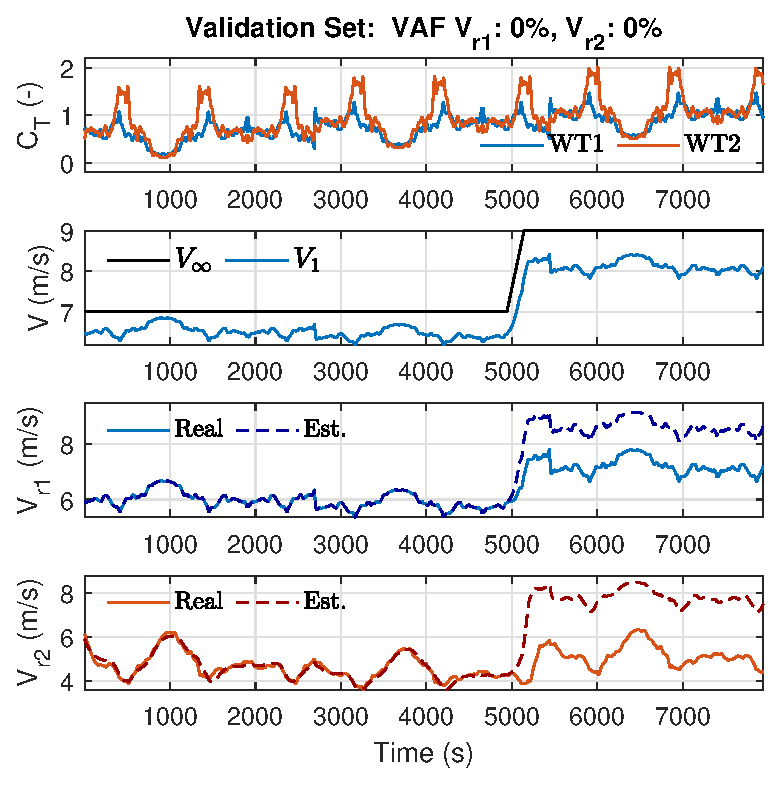
\includegraphics[width=\textwidth]{figures/figures_CDC22/Fig01_OL_Update0_tex.eps}
            \vspace{0.4cm} 
        \end{minipage}
    }\hfill 
    \subfloat[Online-updated model]{
        \begin{minipage}[b]{0.485\textwidth}
            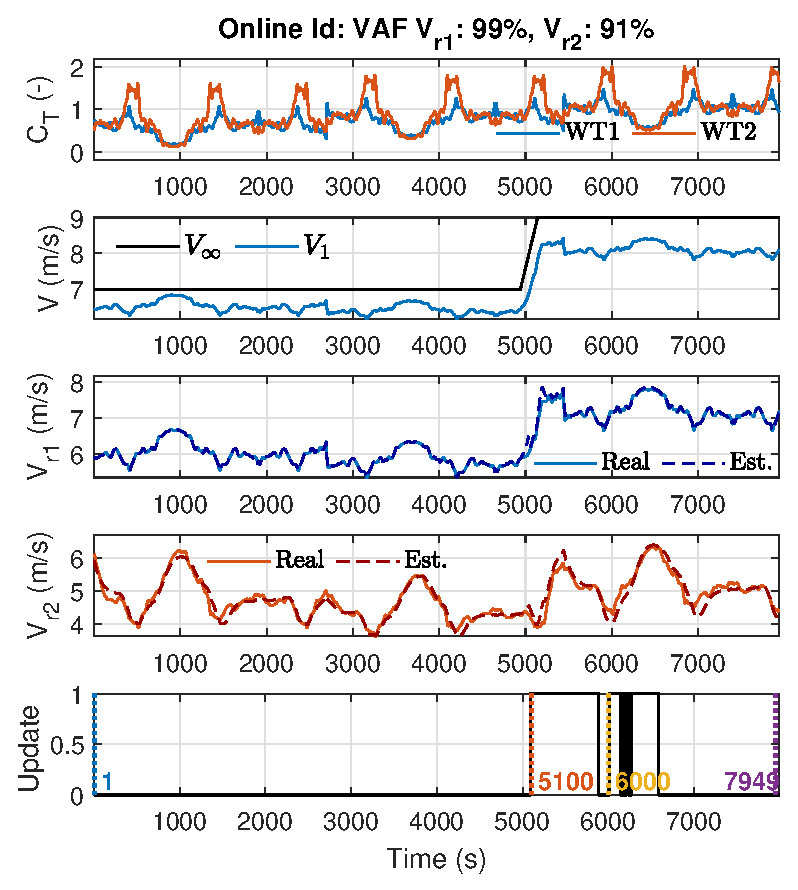
\includegraphics[width=\textwidth]{figures/figures_CDC22/Fig02_OL_Update1_tex.eps}
        \end{minipage}
    }
    \caption[Open-loop identification comparison during a wind speed step]{Open-loop identification comparison during a wind speed step at $t=5000$\,s. Subplots (top to bottom): thrust $C_T$; wind speeds $V_\infty$ (black) and $V_1$ (blue); and real vs. estimated effective wind $V_{r1}, V_{r2}$. Bottom plot in (b) shows the update signal (black). WT1/WT2 signals are blue/red; dashed lines denote estimates.}
    \label{fig:ValComp}
\end{figure}

To quantify the model's accuracy, the Variance Accounted For (VAF) is utilized to measure the similarity between the simulated and estimated effective wind speeds. This measure of how well the output signal variation is explained by the model is also used in previous studies on Koopman DMD, e.g., \cite{Cassamo.2020}, and is defined as:
\begin{equation}
    \text{VAF} = \max \left(0, \left( 1 - \frac{\operatorname{var}(\bm{X} - \hat{\bm{X}})}{\operatorname{var}(\bm{X})} \right) \right)  \cdot 100\%
\end{equation}
where $\bm{X}$ is the simulated or real signal, $\hat{\bm{X}}$ is the estimated signal, and $\operatorname{var}(\cdot)$ denotes the variance. 

The first subplot in Figure~\ref{fig:ValComp}(a) shows the thrust control signals (blue for Turbine WT1, red for Turbine WT2). The second plot shows the freestream wind speed in black and the wind measured directly in front of the first turbine in blue. The third and fourth plots display the simulated effective wind speeds as solid lines and the estimated values as dashed lines. Up to the wind speed change at $t = 5000\,\mathrm{s}$, the estimates follow the real data accurately. However, after the step, the model fails to predict the effective wind speed, resulting in a significant offset and an overall VAF of $0\%$ for both signals. In contrast, Figure~\ref{fig:ValComp}(b) presents the results from the online update scheme applied to the same dataset. With adaptation enabled, the estimated effective wind speeds $V_{r1}$ and $V_{r2}$ achieve VAFs of 99\% and 91\%, respectively. While the first four subplots display the same categories of signals as Figure~\ref{fig:ValComp}(a), the fifth subplot explicitly illustrates the update trigger logic. This plot indicates the instances where the model is updated because the discrepancy between the most recent five real and estimated data points exceeded the threshold $\nu$.

%\begin{figure}[ht]
%    \centering
%    \includegraphics[width=0.65\textwidth]{figures_CDC22/Fig02_OL_Update1_tex.eps}
%    \caption{Open-loop system identification using the online-updated Koopman model during a wind speed step change.}
%    \label{fig:Valonline}
%\end{figure}

Figure~\ref{fig:SingVal} depicts the maximum and minimum singular values of four linear Koopman models at different stages of the online update process. The black dashed line represents the result of a system identification performed offline using the complete dataset from the second open-loop simulation, which includes the wind speed step. The colored solid lines correspond to the singular values of specific update instances at sample index $k$, which are highlighted using matching colors in the fifth subplot of Figure~\ref{fig:ValComp}(b). The initial model (blue line) is calculated on the dataset of the first open-loop simulation that does not contain the wind speed step. Note that with a sampling interval of $t_k = 1$\,s, the index $k$ corresponds directly to the simulation time in seconds. Singular values represent the gain of a system over a frequency range, with the maximum and minimum singular values defining the bounds of the system's amplification of input signals. Investigating these trajectories allows for an assessment of how the identified dynamics evolve, as shifts in the singular values indicate that the model is successfully capturing the underlying system's frequency response under varying operating conditions.
\begin{figure}[ht]
    \centering
    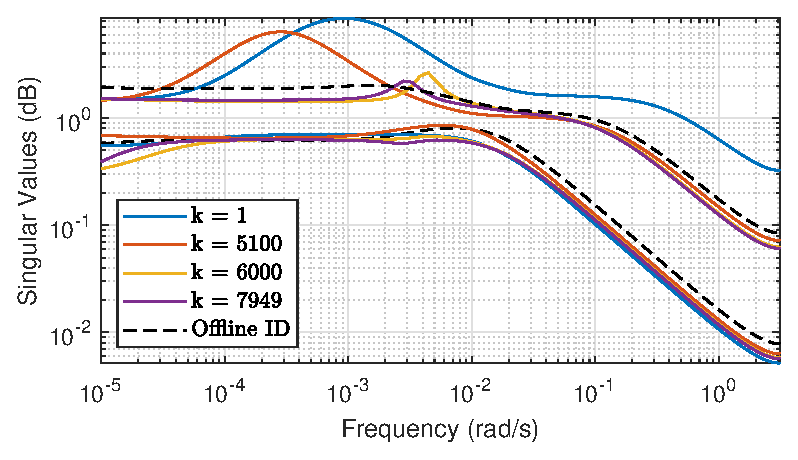
\includegraphics[width=0.65\textwidth]{figures/figures_CDC22/Fig03_OL_Bode_tex.eps}
    \caption[Maximum and minimum singular values of the Koopman models at various sample steps $k$ during online identification].{Maximum and minimum singular values of the Koopman models at various sample steps $k$ during online identification. The shift from the initial model (blue) to the final adapted model (purple) demonstrates the convergence of the model's frequency response toward the reference offline identification (dashed black) following the wind speed step change.}
    \label{fig:SingVal}
\end{figure}

\begin{itemize}
    \item The blue line ($k = 1$) represents the initial Koopman model identified at $V_{\infty} = 7\,\mathrm{m/s}$. Its frequency response differs significantly from the reference offline model (black dashed line). As this initial model was identified using data with a constant freestream wind speed, it lacks the low-frequency excitation necessary to capture steady-state gains. This results in a 'hump' at $10^{-3}$\,rad/s.
    \item The red line ($k = 5100$) shows the model immediately after the wind speed step at $5000\,\mathrm{s}$. Following the wind speed step, the identification process uses data with low-frequency content due to the change in freestream wind, causing the singular values to converge toward the low-pass behavior seen in the offline reference model. While the elevation in the low frequency range is still considerably visible in the red line, its decrease compared to the blue line indicates the adaptation to the new operating point.
    \item The yellow line ($k = 6000$) illustrates the model during the transition as more data from the $9\,\mathrm{m/s}$ regime is incorporated.
    \item The purple line ($k = 7949$) represents the final adapted model, showing a high degree of correlation with the reference offline model across the relevant frequency range.
\end{itemize}


The subsequent section presents closed-loop results obtained from WFSim using the adaptive Koopman model to provide effective wind speed estimates to the qLMPC controller. The value for the triggering condition $\nu$ was set to 0.15\,m/s which was found to be a good compromise between the number of updates and the accuracy of the estimation.

\subsubsection{Closed Loop Results}
A test case is implemented to demonstrate the benefits of the adaptive Koopman MPC algorithm versus the non-adaptive scheme. The simulation is run for $5000$\,s, resulting in a dataset of $5000$ samples. At sample $k = 2000$, the freestream wind $V_\infty$ increases from $7$\,m/s to $9$\,m/s with a ramp of $0.1$\,m/s per sample. The farm power reference $P_{\text{ref}}$ is increased in a step change from $1.72$\,MW to $2.58$\,MW at sample $k = 2500$. These values were selected to ensure the wind farm is physically capable of meeting the power demand at the given wind speeds.

The closed-loop performance is quantitatively evaluated using the Tracking Error (TE) and Actuator Activity (AA). While the Variance Accounted For (VAF) metric was previously used to validate the model's open-loop predictive accuracy, it is less suited for evaluating control success. In closed-loop operation, the primary objectives are to minimize the deviation from the power reference and reduce mechanical wear. Therefore, TE and AA are used as they directly correspond to the cost function terms minimized by the controller, as defined in Equation~\eqref{eq:NMPCcostAIC}. The specific weighting matrices $Q$ and $R$ used in the MPC cost function are provided in the title of Figure~\ref{fig:CL_Comparison}.

Figure~\ref{fig:CL_Comparison} compares the performance of the non-adaptive (a) and adaptive (b) Koopman MPC schemes.

\begin{figure}[ht]
    \centering
    % Subfigure (a): No online update
    \subfloat[Non-adaptive Koopman MPC]{
        \begin{minipage}[b]{0.485\textwidth}
            \centering
            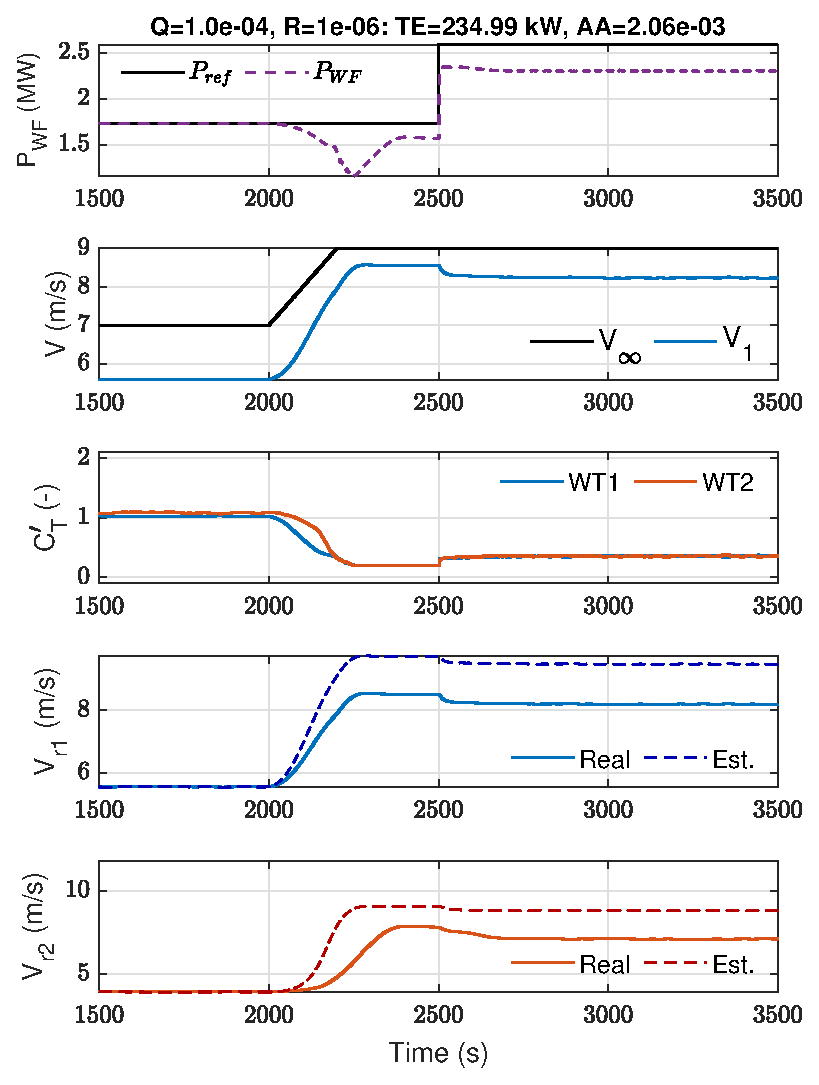
\includegraphics[width=\textwidth]{figures/figures_CDC22/Fig04_CL_Update0_tex.eps}
            \vspace{-0.35cm} 
        \end{minipage}
    }\hfill 
    % Subfigure (b): Online update
    \subfloat[Adaptive Koopman MPC with online updates]{
        \begin{minipage}[b]{0.485\textwidth}
            \centering
            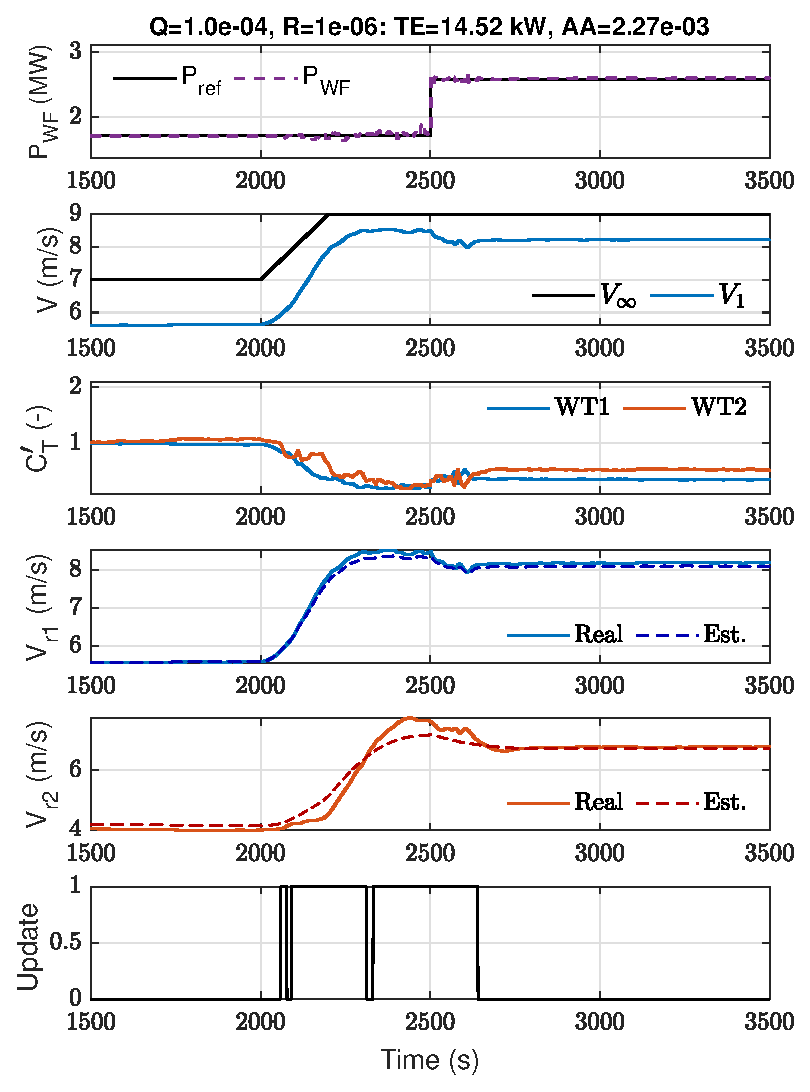
\includegraphics[width=\textwidth]{figures/figures_CDC22/Fig05_CL_Update1_tex.eps}
        \end{minipage}
    }
    \caption[Closed-loop tracking comparison during a wind speed ramp and power reference step.]{Closed-loop tracking comparison during a wind speed ramp and power reference step. Subplots (top to bottom): reference $P_{\text{ref}}$ (black) and total power $P_{\text{WF}}$ (purple dashed); wind speeds $V_\infty$ (black) and $V_1$ (blue); thrust $C_T$; and real vs. estimated effective wind $V_{r1}, V_{r2}$. Bottom plot in (b) shows the update signal (black). WT1/WT2 signals are blue/red; dashed lines denote estimates.}
    \label{fig:CL_Comparison}
\end{figure}

The top subplots illustrate the farm-level power yield $P_{\text{WF}}$ (purple) relative to the reference signal $P_{\text{ref}}$ (black). The subsequent subplots display the freestream wind speed $V_{\infty}$ alongside the local wind speed $V_1$ measured at turbine WT1, followed by the thrust control inputs $C_{T1}$ and $C_{T2}$. Consistent with the previous identification plots, signals for WT1 are shown in blue and WT2 in red. The fourth and fifth rows compare the true effective wind speeds $V_{r1}, V_{r2}$ with their estimates, while the final subplot in Figure~\ref{fig:CL_Comparison}(b) indicates the specific instances where the Koopman model was updated online.

As shown in the first subplot of Figure~\ref{fig:CL_Comparison}(a), the non-adaptive scheme significantly overestimates the effective wind speeds following the transition. This leads to insufficient thrust coefficients $C_{T1}$ and $C_{T2}$, resulting in a large power tracking offset of $234.99$\,kW. In contrast, the online-updated model in Figure~\ref{fig:CL_Comparison}(b) reduces this offset to $14.52$\,kW. The adaptive scheme successfully tracks the effective wind speed despite changes in both the disturbance signal ($V_{\infty}$) and the power reference ($P_{\text{ref}}$).

However, a small increase in actuator activity is observed in the adaptive case. This is due to a persistent excitation signal added to the thrust coefficient to ensure the data remains informative for online identification. When the update condition is triggered, white noise is added to the control signal, updated every five samples. This augmented signal is a weighted sum of the optimal control input and the noise (weighted $0.99$ and $0.01$, respectively), ensuring that power tracking quality is maintained while satisfying the requirements for efficient online adaptation.

It should be noted that the highly precise and nearly instantaneous power tracking achieved by the adaptive Koopman MPC is partly attributable to the simplified modeling assumptions within the WFSim environment. Specifically, the simulation does not account for internal structural mechanics, rotational inertia, or actuator dynamics, instead representing the wind turbines as controlled energy sinks. In a higher-fidelity setup that incorporates these physical properties, the tracking response would likely be more restricted by mechanical time constants and the structural load limitations of the turbine hardware. Consequently, while these results demonstrate the superior adaptive capabilities of the Koopman-based approach, further validation using aeroelastic tools would be necessary to assess performance under realistic mechanical constraints.

 Nonetheless, this adaptive Koopman approach demonstrates that effective wind speeds in highly nonlinear wake environments can be accurately estimated and tracked online. By selectively updating the model only when new information is present, the framework maintains high estimation accuracy, with VAF values consistently around 90\% in both open- and closed-loop scenarios. In the closed-loop tracking case, the adaptive strategy significantly outperforms the non-adaptive scheme, reducing power tracking error while maintaining acceptable actuator activity. These results validate the use of adaptive Koopman models as a solid foundation for wind farm control under varying freestream conditions. The following section builds upon this framework by integrating yaw control, exploring how WRC can be used alongside thrust control to further optimize total farm yield.



% This adaptive Koopman based approach for modelling highly
%nonlinear wakes hence estimates effective wind speed acting
%on wind turbines in a wind farm. An update rule is
%presented to enable online learning only when discrepancies between measurements and model estimates show that
%new measurements contain new information. Additionally,
%to provide sufficient information for the online update a
%small excitation test signal is superimposed on the control
%input if the update of the Koopman model is triggered. The
%WFSim environment was enhanced to support the use of
%changes in wind speed and used to generate test signals
%for open loop identification as well as a test environment
%for the designed controller. High VAF accuracies of wind
%estimations, around 90\%, were observed both in open and
%in closed loop. 
%In closed loop, the adaptive online-update strategy tracked the reference farm power well, outperforming recently presented non-adaptive schemes. Building on these promising results of applying adaptive Koopman models for wind farm control, possible future research directions are employing more realistic wind scenarios, including wind direction variations and the integration of yaw control. The next section discusses the inclusion of yaw control, as wake redirection control (WRC) represents a promising method to further increase overall wind farm yield.

\section{Wind Farm MPC with Combined Yaw and Thrust Control} 
\label{sec:WindFarmLinearMPCforWRC-AIC}

The control design presented in Section~\ref{sec:AdaptiveWindFarmqLMPCforAIC} is extended to include yaw control in addition to thrust control. Two data-driven WRC-AIC wind farm control approaches based on Koopman model predictive control are proposed and compared to a baseline AIC scheme. These WRC-AIC algorithms combine thrust and yaw control for power reference tracking and yield optimization:
\begin{enumerate}
    \item \textbf{Koopman wind estimation:}  
    The upstream turbine's yaw angle is computed to maximize power yield, while the thrust control signals of both turbines are determined via quasi-linear model predictive control (qLMPC) to minimize power tracking error and thrust variations. Both control actions are based on estimated effective wind speeds obtained from a Koopman model identified from open-loop WFSim data, using the control signals as inputs and the two effective wind speeds as outputs, as described in Section~\ref{sec:AdaptiveWindFarmqLMPCforAIC}.
    
    \item \textbf{Koopman farm power estimation:}  
    The upstream turbine's yaw angle and thrust coefficients are optimized simultaneously via linear MPC to minimize power tracking error as well as variations in thrust and yaw. In this case, the controller operates directly on the estimated total farm power, which is derived from a separate Koopman model identified with the same inputs as the first model but with the total wind farm power as the output.
\end{enumerate}
The first approach follows the concept introduced in \cite{boersma2017tutorial}. It verifies whether the power reference exceeds the so-called greedy power of the wind farm, defined as the power obtained when both turbines operate without yaw misalignment and at maximum thrust. If this condition is met, the yaw angle is gradually increased to an offline-calculated value that maximizes the overall wind farm yield. The second approach investigates whether smoother control signals can be achieved by jointly optimizing all available control inputs.

The test case corresponds to the same wind farm setup consisting of two turbines introduced in Section~\ref{sec:WindFarmSimulationWFSim} and used in Section~\ref{sec:AdaptiveWindFarmqLMPCforAIC}, with the wind direction aligned with the main axis of the farm. The two Koopman MPC designs leveraging combined WRC-AIC significantly reduce the tracking error compared to the previously presented baseline AIC algorithm. It is also demonstrated that this improvement can be achieved with relatively small yaw angles, thereby avoiding excessive mechanical loads on turbines operating with yaw misalignment. This makes the proposed approach a promising candidate for further investigation in three-dimensional medium- and high-fidelity simulation environments.

%
\subsection{Simulation Setup for Combined Yaw and Thrust Control} \label{WakeModel} 
As before, WFSim is used to obtain open-loop data and for closed-loop controller testing. This section provides an overview of the WFSim environment and describes the specific test cases utilized for Koopman system identification in this context.

Figure~\ref{fig:BlockDiagramFarm} illustrates the underlying concept for the WRC-AIC strategies applied to the two-turbine wind farm. Note that the primary difference from the setup in Section~\ref{sec:AdaptiveWindFarmqLMPCforAIC} is that the yaw control signal of the upstream turbine WT1, $\gamma_1$, is now an active control variable.

\begin{figure}[h]
    \centering
    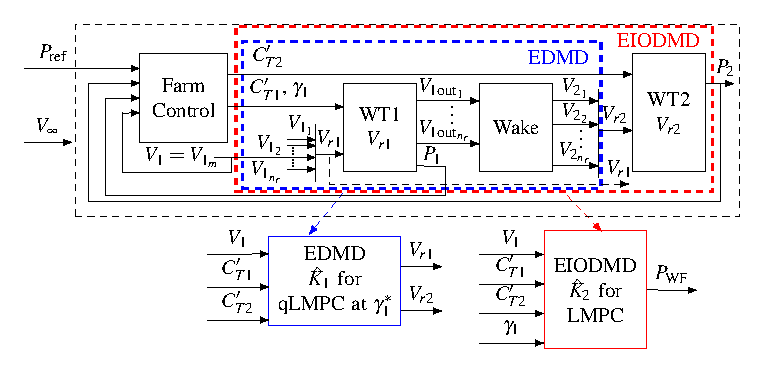
\includegraphics[width=0.9\textwidth]{figures/figuresBlockDiagram_IFAC23/farmCtrl17_P_multVthesis_WRCAIC_EIODMD.pdf}
    \caption[Block diagram of WFSim for WRC-AIC]{Block diagram of WFSim for WRC-AIC with farm control inputs $P_{\text{ref}}$, $P_1$, $P_2$, and $V_1 = V_{1_m}$, control signals $C_{T1}^{\prime}$, $C_{T2}^{\prime}$, $\gamma_1$, and freestream wind $V_\infty$. Local wind speeds upwind and downwind of WT1 are $V_{1_1} \dots V_{1_{n_r}}$ and $V_{1\text{out}_1} \dots V_{1\text{out}_{n_r}}$. Wind speeds upwind of WT2 are $V_{2_1} \dots V_{2_{n_r}}$. The input to the EDMD model (blue) are $V_1, C_{T1}^{\prime}, C_{T2}^{\prime}$ with effective wind outputs $V_{r1}, V_{r2}$. The input to the EIODMD model (red) are $V_1, C_{T1}^{\prime}, C_{T2}^{\prime}, \gamma_1$ with farm power output $P_{\text{WF}} = P_1 + P_2$.}
    \label{fig:BlockDiagramFarm}
\end{figure}

The signals are defined as in previous sections, with the exceptions that the freestream wind speed is kept constant and $\gamma_1$ is commanded by the farm controller. This results in the following signal configuration:
\begin{description}
    \item[-] The freestream wind $V_\infty$ is constant at $8$\,m/s and aligned perpendicular to the turbines for all simulations in this section.
    \item[-] The farm power reference $P_{\text{ref}}$.
    \item[-] The measured wind $V_1$ at WT1, used as a controller input as established in Section~\ref{sec:AdaptiveWindFarmqLMPCforAIC} and the underlying study~\cite{dittmer2022data}.
    \item[-] The thrust control signal $C_{T1}^{\prime}$ and yaw $\gamma_1$ of WT1, with the latter being a variable here, while it was fixed at $0$\,deg in Section~\ref{sec:AdaptiveWindFarmqLMPCforAIC}.
    \item[-] The effective wind speed $V_{r1}$ (mean wind speed over the rotor disk) and power $P_1$ of WT1.
    \item[-] Corresponding input and output signals for turbine WT2.
\end{description}
The farm layout and turbine parameters follow Table~\ref{table:WfSim}. For EDMD, estimates $\Tilde{U}_{ri}$ are calculated from $P_i$ assuming a known power coefficient $c_p$.

Previous publications utilizing WFSim~\cite{boersma2017tutorial,doekemeijer2018online, sharan2022Koopman, dittmer2022data} focused on thrust control $C_T^{\prime}$ for AIC, resulting in $n_u = n_{\text{WT}}$ control inputs. However, WFSim also supports yaw control $\gamma$ for wake redirection. In a two-turbine scenario, this could result in $2n_{\text{WT}}$ inputs; however, for this proof of concept, only the yaw of the first turbine is varied. Since the second turbine has no downstream neighbors, its optimal orientation remains $\gamma_2 = 0$\textdegree{}, resulting in $n_u = 3$ control inputs for this study.

Open-loop data is acquired from a WFSim simulation of $n_o = 28000$ samples, where one sample $k$ corresponds to $1$\,s. The thrust signals $C_{T1}^{\prime}$ and $C_{T2}^{\prime}$ are constructed from white noise (mean 1.7, variance 0.3, lower and upper limits 0.1 and 2.0, respectively) held constant for $5$\,samples. The yaw signal $\gamma_1$ is stepped by $5$\textdegree{} every $4000$\,samples from $0$\textdegree{} to $30$\textdegree{} and augmented with zero-mean band-limited noise (variance $0.5$\textdegree{}). These signals ensure data excitation across all relevant frequencies and control input combinations.

The matrices $\bm{X}_{\text{EIODMD}}$ and $\bm{X}_{\text{EIODMD},+}$ are constructed from input, state and output samples:
\begin{equation}
    \bm{w}(k) = \begin{bmatrix} C_{T1}'(k) \quad C_{T2}'(k) \quad \gamma_1(k) \end{bmatrix}^T, \quad \bm{x} = [V_{r1} \;\; V_{r2}]^T,  \quad 
    \bm{y}(k) = P_{\text{WF}}(k).
\end{equation}
and are assembled by stacking snapshots as follows:
\begin{align}
    \bm{X}_{\text{EIODMD}} &= \bigl[ [\bm{x}(k)^T \quad \bm{w}(k)^T]^T \bigr]_{k=1}^{n_o-1}, \\
    \bm{X}_{\text{EIODMD},+} &= \bigl[ [\bm{x}(k+1)^T \quad \bm{y}(k)^T]^T \bigr]_{k=1}^{n_o-1},
\end{align}

These matrices are used to construct two Koopman matrices, $\hat{K}_1$ (EDMD) and $\hat{K}_2$ (EIODMD), for the respective MPC designs. The system dynamics are of $6^{\text{th}}$ order with:
\begin{description}
    \item[-] Lifted states $\bm{\varphi} = [\bm{x}^T \;\; (\bm{x}^2)^T \;\; (\bm{x}^3)^T]^T$. The quadratic and cubic terms reflect the relationship between wind, force and power.
    \item[-] Inputs $w_{K1} = [C_{T1} \;\; C_{T2} \;\; V_1]^T$ and $w_{K2} = [C_{T1} \;\; C_{T2}'\;\; V_1\;\; \gamma_1]^T$.
    \item[-] EDMD outputs $\bm{y}_{K1} = [V_{r1} \;\; V_{r2}]^T$ and EIODMD outputs $\bm{y}_{K2} = P_{\text{WF}}$.
\end{description}

The matrix $\hat{K}_{w2} \in \mathbb{R}^{7\times11}$ is reordered to separate the contributions of the system states via the matrices $A_w \in \mathbb{R}^{6\times6}$ and $C_w \in \mathbb{R}^{1\times6}$, control inputs via $B_u \in \mathbb{R}^{6\times3}$ and $D_u \in \mathbb{R}^{1\times3}$, and the measured disturbance input $V_1$ via $B_d \in \mathbb{R}^{6\times1}$ and $D_d \in \mathbb{R}^{1\times1}$. To account for the disturbance as a state in the linear MPC, the matrices are augmented, resulting in the state-space matrices $A_{\hat{K}2} \in \mathbb{R}^{7\times7}$, $B_{\hat{K}2} \in \mathbb{R}^{7\times3}$, $C_{\hat{K}2} \in \mathbb{R}^{1\times7}$, and $D_{\hat{K}2} \in \mathbb{R}^{1\times3}$. The relationship to the original matrices obtained from EIODMD is given by:

\begin{align*} 
    \hat{K}_{w2} = \left[\begin{array}{c|cc} 
        A_w & B_d & B_u\\ 
        \hline 
        C_w & D_d & D_u 
    \end{array}\right] \implies
    \hat{K}_{2} = \left[\begin{array}{cc|c} 
        A_w & B_d & B_u\\ 
        \bm{0}_{1\times6} & 1 & \bm{0}_{1\times3}\\
        \hline 
        C_w & D_d & D_u 
    \end{array}\right].
\end{align*}

The specific formulation and implementation of the qLMPC (based on $\hat{K}_1$) and linear Koopman MPC (based on $\hat{K}_2$) are detailed in Section~\ref{qLMPCDesign}.
%with state vector $\bm{x} = [V_{r1}\;\;V_{r2}]^T  $, input vector  $\bm{w} = [V_{r1}\;\;V_{r2}]^T  $
%The collected WFSim simulation signals are then used to calculate a Koopman matrix $\hat{K}_w$ via EIODMD,  as bases for the the MPC design. The system dynamics of the identified systems are of 6$^{th}$ order with 
%\begin{itemize}
%\begin{description}
%\item[-] inputs $w_{K1}$ as controls $C_{T1}^{\prime}$ and $C_{T2}^{\prime}$ and disturbance $V_1$, inputs $w_{K2}$ as all inputs $w_{K1}$ and additional control input $\gamma_1$
%\item[-] inputs $\bm{w}$ as control inputs $C_{T1}^{\prime}$, $C_{T2}^{\prime}$ and $\gamma_1$ and disturbance wind $V_1$,
%    \item[-] outputs of the EDMD wind estimation model as effective wind speeds, i.e. $y_{K1} = x = [V_{r1},V_{r2}]$
%\item[-] and outputs of the EIODMD power estimation model as farm power $y_{K2} = P_{\text{WF}} = P_1 + P_2$.
%\end{description}
%The values in the identified matrix $\hat{K}_w \in \mathbb{R}^{7\times10}$ are reordered to find the optimal three control inputs given measured wind $V_1$ and a power reference, both assumed constant over the prediction horizon. Hence, there is one additional disturbance state and three control inputs, resulting in augmented state $ \zeta_d = [\zeta^T  , V_1]^T   $ and matrices $\hat{K} \in \mathbb{R}^{8\times10}$, $A_{\hat{K}} \in \mathbb{R}^{7\times7}$, $B_{\hat{K}}\in \mathbb{R}^{7\times3}$, $C_{\hat{K}}\in\mathbb{R}^{1\times7}$, and $D_{\hat{K}}\in\mathbb{R}^{1\times3}$:


%$[\dot{x}_{K2},\dot V_1] = [A,B_d;0^{1\times7}] [x_{K2}, V_1]^T   + B_{K2} w $
%The matrix $Tilde(K)_2$, the result of the system identification with inputs $w_{K2}$ and output $$
\subsection{MPC Design for Combined Yaw and Thrust Control} \label{qLMPCDesign} 
Similar to the previously discussed AIC algorithm, the objective of the WRC-AIC wind farm controllers is to achieve accurate power reference tracking while minimizing changes in the control inputs. The WRC-AIC extends the previous approach by including the yaw of the first turbine as an additional control input, alongside the already used thrust control signals, which requires adjustments to the objective function and control algorithm. The main benefit of incorporating yaw, which is an increase in the achievable wind farm power output, will be demonstrated in the results presented in Section~\ref{SimResults}. In this section, the cost function to be optimized is defined, and the two MPC designs based on the Koopman matrices $\hat{K}_1$ and $\hat{K}_2$ are discussed.

The cost function $J(\bm{U})$ for both WRC-AIC schemes is formulated identically to the AIC algorithm, as given in Equation~\eqref{eq:errortraject}. It is based on the trajectories of the tracking error $\bm{E}$ and the changes in the control input $\Delta \bm{U}$:
\begin{align*} 
    J(\bm{U}) = \underbrace{\bm{E}^T \bm{Q} \bm{E}}_{J_Q (\bm{U})} + \underbrace{\Delta \bm{U}^T \bm{R} \Delta \bm{U}}_{J_R (\bm{U})},
\end{align*}
over a prediction horizon of $n_h$ sample steps. The weighting matrices are based on the scalar weights $Q$ and $R$, with the weight on the power error derived as $\bm{Q} = Q \bm{I}^{n_h \times n_h}$, as before. The weight on the control input changes is defined as
\begin{align*}
    \bm{R} = R \cdot \mathrm{diag}(R_{u1}, R_{u2}, \dots, R_{n_u}) \otimes \bm{I}^{n_h \times n_h},
\end{align*}
allowing differentiation of the penalty on changes in the different control inputs.

Correspondingly, the future error trajectory is $\bm{E}_k = \bm{P}_{\text{ref},k} - \bm{P}_{\text{WF},k}$, which is based on the total wind farm power. The change in control inputs is calculated as in Equation~\eqref{eq:UandDUAIC}.

For the two turbines considered and the default WFSim setting $n_h = 10$, the dimension of the control trajectory differs between the two approaches:
\begin{itemize}
    \item qLMPC approach ($\hat{K}_1$): The yaw angle $\gamma_1$ is optimized offline and kept as a static parameter during the control interval. Thus, only the two thrust signals are active control inputs, i.e., $n_u = 2$. This results in a trajectory $\Delta \bm{U}_{K1} \in \mathbb{R}^{20}$, as 2 inputs are optimized over 10 prediction trajectory steps.
    \item Linear MPC approach $\hat{K}_2$): The yaw angle $\gamma_1$ is included as a third active control input, resulting in $n_u = 3$. This yields a trajectory $\Delta \bm{U}_{K2} \in \mathbb{R}^{30}$ with 3 inputs set for 10 steps, with the control trajectory defined as:
    \begin{align*} 
        \bm{U}_{K2}(k) &= \begin{bmatrix} 
            C_{T1}^\prime(k) & C_{T2}^\prime(k) & \gamma_1(k) & \dots & \gamma_1(k+n_h-1) 
        \end{bmatrix}^T \in \mathbb{R}^{30 \times 1}.
    \end{align*}
\end{itemize}

For both designs, the cost function summands can be written as:
\begin{align*} 
    J_Q (\bm{U}) &= \big(\bm{P}_{\text{ref}} - (\tilde{\bm{L}} \bm{x}_0 + \tilde{\bm{S}} \bm{U})\big)^T \bm{Q} \big(\bm{P}_{\text{ref}} - (\tilde{\bm{L}} \bm{x}_0 + \tilde{\bm{S}} \bm{U})\big),\\
    J_R (\bm{U}) &= \Delta \bm{U}^T \bm{R} \Delta \bm{U},
\end{align*}
where the initial state $\bm{x}_0 \in \mathbb{R}^{3 n_T}$ is the state from the last sample, and the matrices $\tilde{\bm{L}} \in \mathbb{R}^{n_h \times 3 n_T}$ and $\tilde{\bm{S}} \in \mathbb{R}^{n_h \times n_h n_u}$ are used to calculate the expected future trajectory of the wind farm power $\bm{P}_{\text{WF}}$.

In the EDMD approach using $\hat{K}_1$, the original WFSim qLPV farm model is employed. The optimal yaw $\gamma_1^*$ is computed using the Gaussian wake model from~\cite{bastankhah2016experimental}, ensuring results are comparable to~\cite{boersma2019constrained}. The matrices $\tilde{\bm{L}}_{\hat{K}1}$ and $\tilde{\bm{S}}_{\hat{K}1}$ are calculated from $\bm{A}_{\text{WF}}$ and $\bm{B}_{\text{WF}}(\bm{V}_r)$.

In the EIODMD approach based on $\hat{K}_2$, the wind farm power $\bm{P}_{\text{WF}}$ is estimated directly. This results in a linear MPC, as effective wind speeds are no longer used as scheduling parameters. The stacked Toeplitz matrices $\bm{\Lambda}_{\hat{K}2}$ and $\bm{S}_{\hat{K}2}$ are constructed from the augmented matrices $\bm{A}_{\hat{K}2}, \bm{B}_{\hat{K}2}, \bm{C}_{\hat{K}2}, \bm{D}_{\hat{K}2}$ as:
\begin{align*}
    \bm{\Lambda}_{\hat{K}2} &= \begin{bmatrix}
        \bm{C}_{\hat{K}2} \\
        \bm{C}_{\hat{K}2} \bm{A}_{\hat{K}2} \\
        \vdots \\
        \bm{C}_{\hat{K}2} \bm{A}_{\hat{K}2}^{n_h-1}
    \end{bmatrix}, \quad
    \bm{S}_{\hat{K}2} =
    \begin{bmatrix}
        \bm{D}_{\hat{K}2} & \bm{0} & \dots & \bm{0}\\
        \bm{C}_{\hat{K}2} \bm{B}_{\hat{K}2} & \bm{D}_{\hat{K}2} & \dots & \bm{0}\\
        \vdots & \vdots & \ddots & \vdots \\
        \bm{C}_{\hat{K}2} \bm{A}_{\hat{K}2}^{n_h-2} \bm{B}_{\hat{K}2} & \dots & \dots & \bm{D}_{\hat{K}2}
    \end{bmatrix}.
\end{align*}
Since $\bm{P}_{\text{WF}}$ is the direct output of the EIODMD model, there is $\tilde{\bm{L}}_{\hat{K}2} = \bm{\Lambda}_{\hat{K}2}$ and $\tilde{\bm{S}}_{\hat{K}2} = \bm{S}_{\hat{K}2}$. Note that the inclusion of non-zero elements in the $\bm{D}_{\hat{K}2}$ matrix is a direct consequence of the simplified modeling approach used in WFSim. EIODMD is employed to map control signals directly to farm power without the intermediate scheduling parameter effective wind speed, which was used before. In this case, the relationship between the output power and thrust and yaw inputs is captured including a feedthrough term. This non-zero direct feedthrough reflects the absence of explicit turbine dynamics in the turbine power extraction model.

The next section presents simulation results obtained in WFSim both in open-loop and in closed-loop, using an AIC MPC baseline controller as well as the two MPC controller designs presented above.
%b_{KMPMC2,const} = [b_{const}, \delta u_M \mathbf{1}^{1\times N\cdotn_T}, -\delta u_m \mathbf{1}^{1\times N\cdot n_T}]^T  

%As the cost function is quadratic a reformulation of it as a QP problem gives a perfect reconstruction. Hence, we could show in \cite{adki2021MPC} that we get exactly the same results previously reported regarding power reference tracking performance in \cite{vali2019adjoint}, but with a 15 times speed-up.\\
%The excellent tracking performance is obtained in both \cite{vali2019adjoint} and \cite{adki2021MPC} by providing the effective wind speed of all turbines to the centralized farm controller. As mentioned previously, wind speeds might not be available for all wind turbines of a wind farm. In section \ref{SimResults} it is demonstrated that leveraging only wind estimated via the Koopman model good tracking performance can be achieved without wind measurements using a physically motivated identified model.
%The bounds of the first yaw angle, $u_{m,\gamma} = 0$ and $u_{M,\gamma} = 25$ are included in the vectors $u_m$ and $u_M$ that are used to form the input constraints $A_{c0,K2}$ and $B_{c0,K2}$, otherwise identically to $A_{c,K1}$ and $B_{c,K1}$.
%Moreover, the rate limits $\delta u$ of the rates are included via calculating the differences in rates with $\Delta_R$ with all values of the diagonal set to 1 and all values of the third supra-diagonal set to -1 to subtract the next value of the prediction horizon. In the current design $U^l$ is constant. Hence, the difference between the values of $\tilde{U}$ and $U$ is identical. Therefore, the new constraint matrices are: %for the MATLAB function \textit{quadprog} with linear constraints $A_{c} x < b_{c}$:
%\begin{align*} %\label{eqn:constraint}
%A_{c,K2} &= [ A_{c0,K2}, \Delta_R^T  , -\Delta_R^T  ]^T  \\
%B_{c,K2} &= [ B_{c0,K2},  \mathbf{1}^{1\times N\cdot n_T} \otimes (\delta u_M)^T  , \mathbf{1}^{1\times N\cdot n_T} \otimes (-\delta u_m)^T  ]^T  
%\end{align*}
%\begin{align*}
%[U,\Delta U]^T   - [u_M,u_{r,M}]^T   \le 0 \iff 
% [\tilde{U},\Delta_R \tilde{U}]^T   \le [-U^l,0]^T    + [u_M,u_{r,M}]^T    \\
%- [\tilde{U},\Delta_R \tilde{U}]^T   \le [U^l,0]^T    - [u_m,u_{r,m}]^T   %\\
% -U + u_m \le 0 \iff
%-\tilde{U} \le U^l  - u_m 
%\\&\iff -U\le -u_m 
%U- u_m \ge 0 -U-\left({-u}_M \right)\ge 0\\
% \end{align*}
%with rate limits $u_{r,M}$ and $u_{r,m}$ 

\subsection{Results} \label{SimResults}
Open-loop simulations are used to investigate the potential power increase from WRC and to confirm the consistency between the results from the 2D NSE and the Gaussian wake model. Subsequently, closed-loop simulations are performed to evaluate power reference tracking performance.


\subsubsection{Open-Loop Results}
Open-loop WFSim simulation results to quantify the effect of wake misalignment are obtained for a step-sweep of the yaw angle $\gamma_1$ from 0\textdegree{} to 35\textdegree{} with consecutive increases of 5\textdegree{} every 500 samples, resulting in a total of 4000 samples. During this sweep, the thrust control signals are set to their maximum value of 2 and the freestream wind is held constant at 8\,m/s.

Figure~\ref{fig:WFSimgamma0} visualizes the simulated longitudinal wind in steady state. The WFSim results are overlaid with the Gaussian wake model from \cite{bastankhah2016experimental}, with the centerline plotted as a blue dotted line and the far-field wake expansion as a blue dash-dotted line. The match of the wake expansion at the rotor disc is reasonable. While the deflection angle of the Gaussian wake model in the far-wake region is slightly smaller than that of the 2D NSE model, the main area of speed deficit is nearly identical between the two. 
It should be noted that the wake centerline of a yawed turbine is curled in the near-wake region; therefore, modeling the centerline as a straight line in this region necessarily leads to discrepancies. This effect is addressed in more recent models such as the curled wake model from \cite{martinez2019aerodynamics}  or the Gaussian-Curl-Hybrid model \cite{king2020controls}, but the standard Gaussian wake model is chosen here for its simplicity and to maintain comparability with \cite{boersma2019constrained}. 

Figure~\ref{fig:PowerPerYaw} shows the farm power $P_{\text{WF}}$ as a function of the yaw angle $\gamma_1$ for both the WFSim simulation and the Gaussian wake model.
%
\begin{figure}[ht]
\centering
\subfloat[Longitudinal wind field for $\gamma_1$ at 0\textdegree{} and 20\textdegree{}.]{
    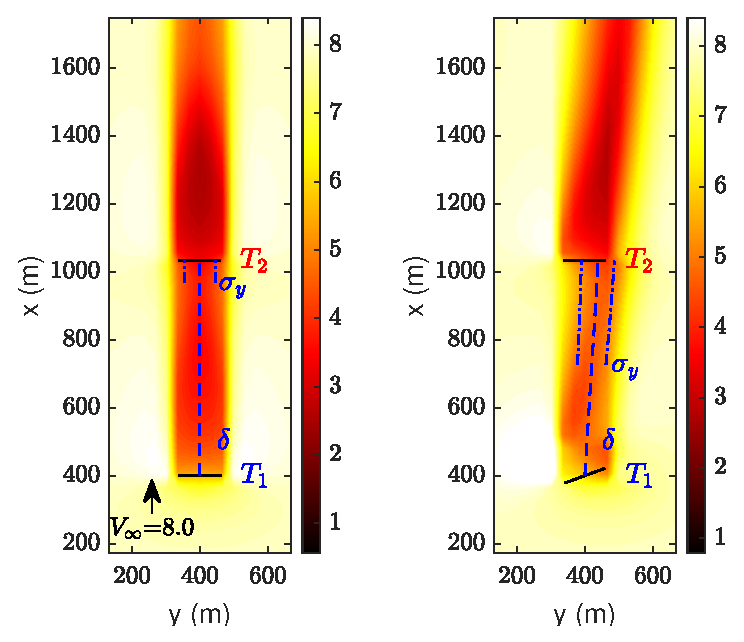
\includegraphics[width=0.48\textwidth]{figures/figures_IFAC23/03FigAngle0_20_tex.eps}
    \label{fig:WFSimgamma0}
}
\hfill
\subfloat[Power $P_{\text{WF}}$ as a function of yaw angle $\gamma_1$.]{
    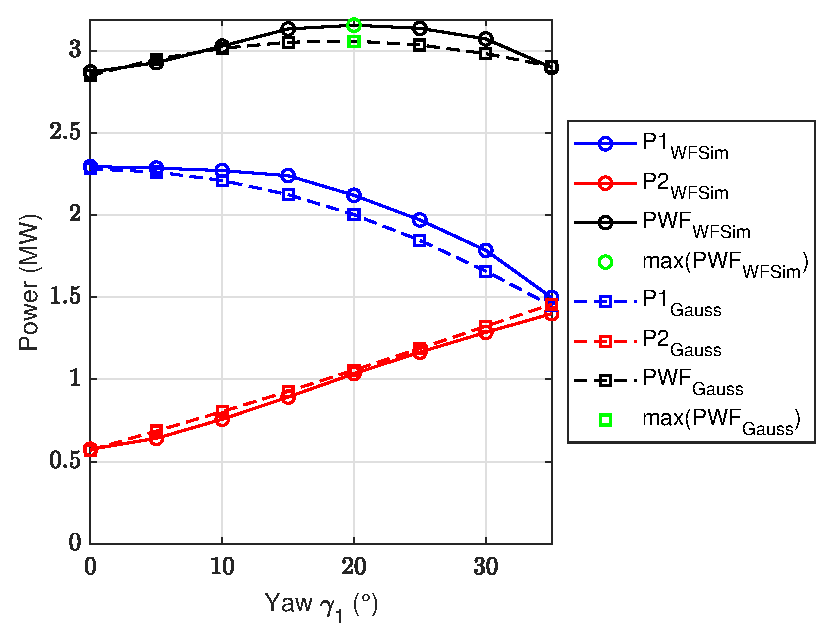
\includegraphics[width=0.48\textwidth]{figures/figures_IFAC23/01FigPwrVsYaw_tex.eps}
    \label{fig:PowerPerYaw}
}
\caption[Open-loop validation of the Gaussian wake model against WFSim.]{Open-loop validation of the Gaussian wake model against WFSim: (a) steady-state longitudinal wind field with Gaussian wake centerline $\delta$ and expansion $\sigma_y$ as blue dashed and dash-dotted lines; (b) power output comparison where WFSim results are marked with circles and the Gaussian model with squares: WT1 (blue), WT2 (red), total wind farm (black), and maximum power point (green)}
\label{fig:OpenLoopResultsCombined}
\end{figure}

The power of the upstream turbine (blue) decreases as the yaw angle increases. This reduction is attributed to the reduced effective rotor area facing the wind and the inherent decrease in aerodynamic efficiency during yawed operations. These effects are analyzed in a comparative study of various yaw models \cite{sant2016comparing} and are further supported by recent field evaluations \cite{hulsman2022turbine}. 

As shown in Figure~\ref{fig:PowerPerYaw}, the simulated power for the first turbine still slightly exceeds the Gaussian wake model predictions between 10\textdegree{} and 30\textdegree{}. Specifically, the farm power increase due to WRC is 10\% in the 2D NSE simulation, compared to 6\% as predicted by the Gaussian model. While this difference in maximum increase is non-negligible, the curves remain in close agreement and both models identify a maximum wind farm yield (green marker on the black curve) at approximately 20\textdegree{} yaw. The fact that the peak occurs at the same angle and that the general curve forms are similar confirms that the Gaussian wake model serves as a computationally efficient and reasonable approximation of the 2D NSE for controller design. % in the qLMPC controller design based on the Koopman model for estimated winds speeds, $Mdl_{K1}$.\\
%It is also worth noting that wake models more recently published then the Gaussian model, namely the curled wake model from  \cite{martinez2019aerodynamics} or the Gaussian-Curl-Hybrid model from \cite{king2020controls} have been demonstrated to yield a better fit to large-eddy simulations and that the Gaussian model underestimating the improvement in power is also reported in these publications. However, the decision was made to use the Gaussian model in this work due to its application to a combination of thrust and yaw control in \cite{boersma2018control}. \cite{boersma2019constrained}
% the deduction from the simulated wind fields

\subsubsection{Closed-Loop Results}
Figure~\ref{fig:ClosedLoopComparison} shows the results of the closed-loop simulations run to evaluate the performance of the baseline AIC controller against the two WRC-AIC designs from Section~\ref{qLMPCDesign}, which incorporate combined yaw and thrust control.
\begin{figure}[h!]
\centering
\subfloat[Baseline AIC ($n_u = 2$) with fixed yaw ($\gamma_1 = 0^\circ$).]{
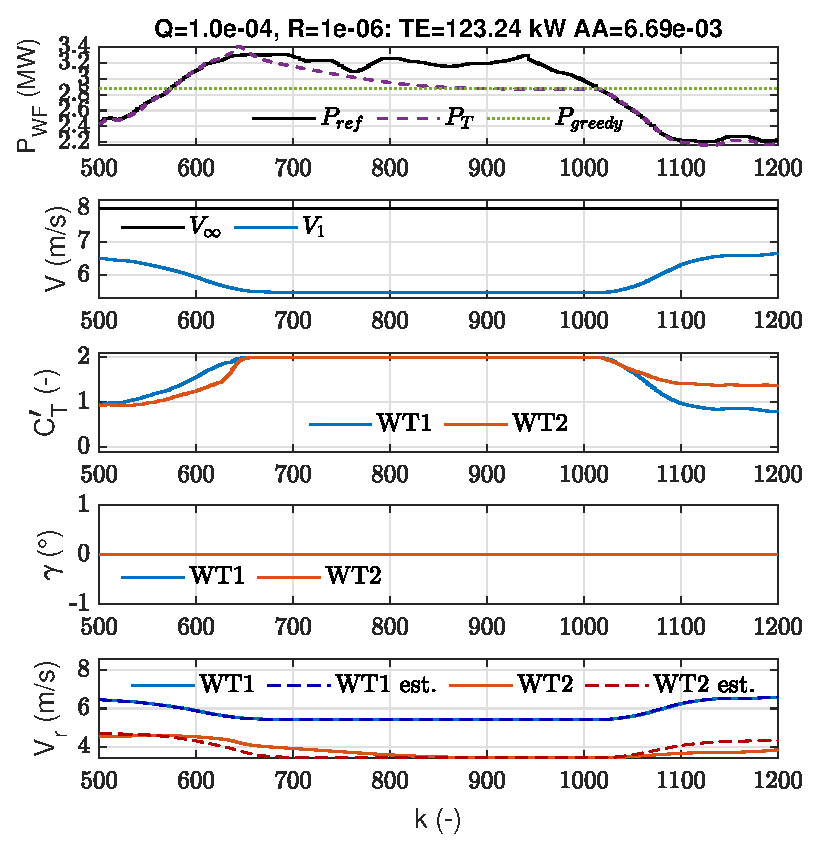
\includegraphics[width=0.48\textwidth]{figures/figures_IFAC23/04FigTimeSeries0_tex.eps}
\label{fig:CLbaseline}
}
\hfill
\subfloat[AIC ($n_u=2$) with pre-optimized yaw ($\gamma_1^* = 18^\circ$) based on Gaussian wake model.]{
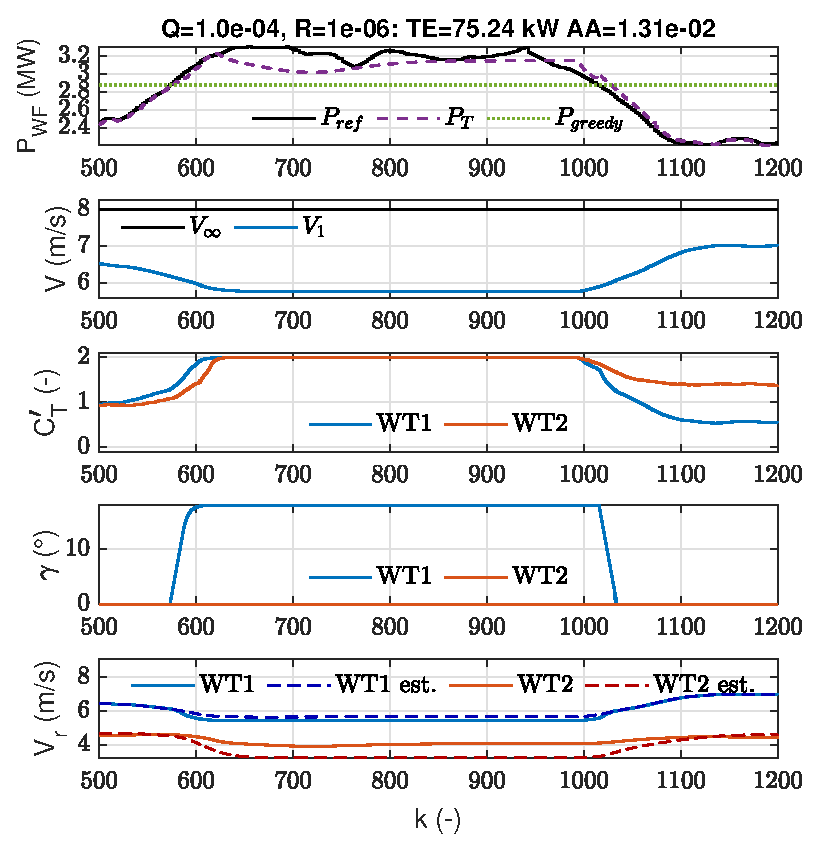
\includegraphics[width=0.48\textwidth]{figures/figures_IFAC23/05FigTimeSeriesQLMPC_tex.eps}
\label{fig:CLMPC1}
}

\vspace{0.5cm} 

\subfloat[WRC-AIC ($n_u=3$): Thrust and yaw controls simultaneously optimized.]{
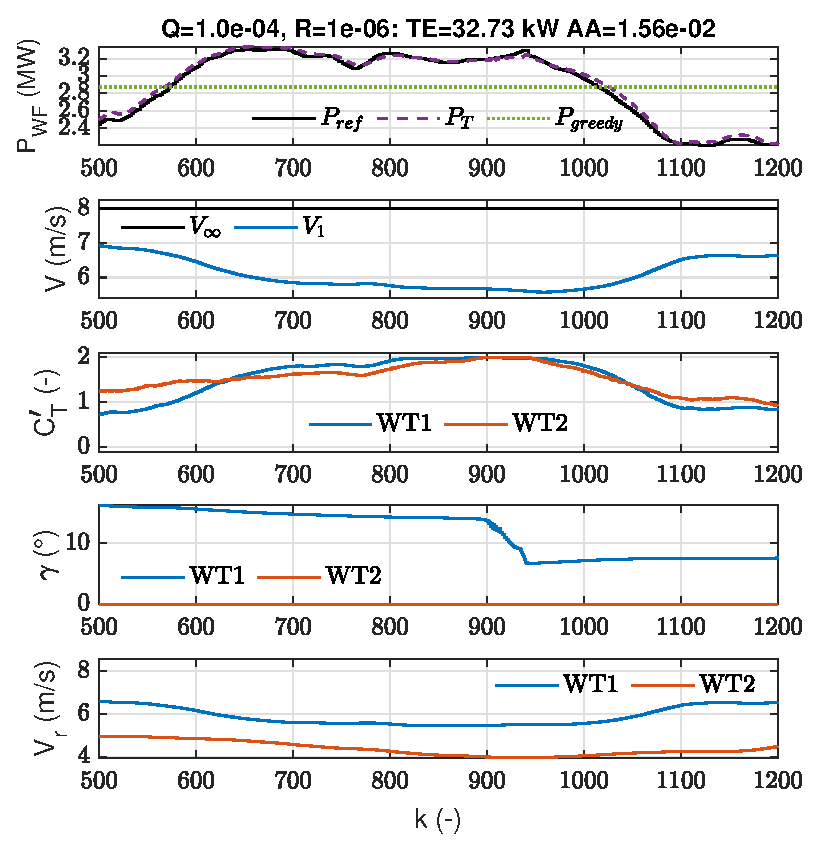
\includegraphics[width=0.48\textwidth]{figures/figures_IFAC23/06FigTimeSeriesLinMPC_tex.eps} 
\label{fig:CLMPC2}
}

\caption[Closed-loop performance comparison baseline AIC and the two WRC-AIC algorithms]{Closed-loop performance comparison baseline AIC and the two WRC-AIC algorithms. Subplots (top to bottom): reference $P_{\text{ref}}$ (solid black) and total power $P_{\text{WF}}$ (purple dashed); wind speeds $V_\infty$ (black) and $V_1$ (blue); thrust $C_T$; yaw $\gamma$; and real vs. estimated effective wind $V_{r1}, V_{r2}$. WT1/WT2 signals are blue/red; dashed lines denote estimates. Weighting parameters: $Q$ and $R$ as provided in subplot titles, $R_{u1}=R_{u2}=1$, and $R_{u3}=0.1$.}
\label{fig:ClosedLoopComparison}
\end{figure}

The controllers are tasked with tracking a dynamic power reference signal, defined as:
\begin{align*}
P_{\text{ref},k} = \big(a_{\text{const}} + a_{\delta} \, \delta P_k \big) P_{\text{greedy}},
\end{align*}
where $P_{\text{greedy}}$ represents the maximum power production of the farm when both turbines operate at maximum thrust ($C_T' = 2$) and zero yaw ($\gamma = 0^\circ$). The reference signal is adapted from the stochastic variation model used in \cite{sharan2022Koopman}. While the original parameters in that study were set to $a_{\text{const}} = 0.8$ and $a_{\delta} = 0.35$, the present work utilizes $a_{\text{const}} = 0.9$ and $a_{\delta} = 0.2$, and the vector $\delta P$ has been resampled to update only every second time step. These modifications are implemented to obtain a reference trajectory that exceeds the greedy power for longer durations, thereby increasing the importance of wake steering for successful trajectory tracking. To ensure the performance metrics are not skewed by initialization artifacts, the evaluation begins at sample $k=240$.

The closed-loop performance is evaluated using the tracking error (TE) and actuator activity (AA) metrics previously introduced in Section~\ref{section:AICWindFarmControl}. These metrics correspond to the weighted components of the cost function in Equation~\eqref{eq:NMPCcostAIC}, where the scalar weights $Q$ and $R$ are specified in the subplot titles of Figure~\ref{fig:ClosedLoopComparison}. 
For the combined control cases, the input-specific weighting factors are set to $R_{u1} = R_{u2} = 1$ for the thrust control inputs $\Delta C_{T1}^\prime$ and $\Delta C_{T2}^\prime$, and $R_{u3} = 0.1$ for the yaw input $\Delta \gamma_1$. Both TE and AA are computed as mean values over the evaluation period (starting at $k=240$), with the AA incorporating the respective weighting factors from the matrix $\bm{R}$. 

Figure~\ref{fig:ClosedLoopComparison}(a) shows the performance of the baseline controller with the yaw angle fixed at zero. Figure~\ref{fig:ClosedLoopComparison}(b) displays results obtained with the first Koopman MPC algorithm ($n_u=2$), which utilizes an optimal yaw setpoint derived from the Gaussian wake model. Finally, Figure~\ref{fig:ClosedLoopComparison}(c) displays the results of the second Koopman MPC algorithm ($n_u=3$), which performs integrated optimization of both thrust and yaw. The first plot in each subfigure shows the power yield at the wind farm level, with the power reference signal $P_{\text{ref}}$ depicted as a solid black line and the power yield $P_{\text{WF}}$ as a dashed purple line. The power $P_{\text{greedy}}$ is depicted as a dashed green line. 

Note in Figure~\ref{fig:ClosedLoopComparison}(a) that when using the thrust coefficient as the only actuator, the power yield initially exceeds the greedy power output if the reference demands it. However, it falls back to the greedy power once the wind speed deficit from the first turbine's maximum thrust reaches the second wind turbine. In Figure~\ref{fig:ClosedLoopComparison}(b), the yaw is increased if the reference power exceeds the greedy power, reducing the tracking error by a factor of 1.8.

In Figure~\ref{fig:ClosedLoopComparison}(c), the tracking error is further reduced from 116\,MW to 33\,MW by including the yaw angle as a third control input. The actuator activity, i.e., the actuator rate, is slightly increased compared to the EDMD design as the overall yaw rate increases. However, the control actuators of the Koopman MPC based on EIODMD result in both smaller thrust coefficient values and a smaller yaw angle value. This is desirable, as it also decreases the forces acting on the tower and blades. 

These results demonstrate that the Koopman-basedWRC-AIC MPC effectively coordinates yaw and thrust to overcome the physical limitations of AIC alone. The following section concludes the chapter by summarizing the key results and discussing the limitations and future research directions for Koopman-based wind farm control.


\section{Conclusions}
This chapter presented and analyzed three applications of DMD using Koopman lifted functions
for wind farm control. The first part discussed the modifications required in the WFSim simulation
environment to enable adaptive control testing and to investigate the influence of intentional yaw
misalignment through a yaw-angle-dependent power coefficient. This was followed by the design,
implementation, and evaluation of an adaptive AIC controller, and subsequently, two WRC-AIC
controllers combining wake redirection and axial induction control.

Table~\ref{tab:WindFarmSummary} summarizes the quantitative evaluation criteria of the
closed-loop simulation runs. The focus of this study was to improve the tracking error, i.e., the
mean difference between the grid demand and the farm power output. The weighted square of
this error is also the first summand of the MPC optimization function. However, the weighting
function also contained the weighted square of the actuator rate. As the original weights from
the simulation environment were not changed, the actuator rate penalty was small relative to
the tracking error weight, allowing rapid thrust changes without penalizing actuator activity.
This results in an increase in actuator activity, i.e., the thrust rate of the rotors increases,
which is most pronounced in the WRC-AIC case. Future research might look into finding a
more balanced approach between decreasing tracking error and limiting actuator activity.

\begin{table}[h]
    \centering
    \caption[Wind farm controller evaluation criteria: Tracking error and
    actuator activity for adaptive AIC (wind speed change) and AIC vs two WRC schemes (challenging power reference).]{Wind farm controller evaluation criteria.
        Tracking error (TE) and actuator activity (AA) for the adaptive AIC
        ( Section~\ref{sec:AdaptiveWindFarmqLMPCforAIC}, wind speed change $V_\infty = 7$--$9$\,m/s)
        and the WRC-AIC algorithms
        (Section~\ref{sec:WindFarmLinearMPCforWRC-AIC}, challenging power reference $V_\infty = 8$\,m/s).
        Results are not directly comparable across sections due to different
        test cases ($Q = 10^{-4}$, $R = 10^{-6}$).}
    \label{tab:WindFarmSummary}
    \begin{tabular}{ll rr}
        \toprule
        Section & Controller & TE (kW) & $\text{AA} / 10^{-3}$\,(-) \\
        \midrule
        \multirow{2}{*}{AIC}
        & Baseline, non-adaptive AIC  & 234.99 & $2.06$ \\
        & Adaptive AIC                &  14.52 & $2.27$ \\
        \midrule
        \multirow{3}{*}{WRC-AIC}
        & Baseline AIC ($\gamma_1 = 0^\circ$)              & 123.24 & $6.69$ \\
        & AIC + Gaussian yaw ($\gamma_1^* = 18^\circ$)     &  75.24 & $13.1$ \\
        & WRC-AIC EIODMD ($n_u = 3$)                       &  32.73 & $15.6$ \\
        \bottomrule
    \end{tabular}
\end{table}

The results highlight several important findings. Physics-informed lifting functions were shown
to effectively capture both the relationship between control inputs and effective wind speeds and
the mapping from control inputs to power outputs. Furthermore, it was demonstrated that
Koopman-based estimation models can be updated online in real time, enabling adaptive control
under non-stationary wind conditions. The inclusion of WRC led to a notable increase in total
farm power output---exceeding 5\%. Specifically, the Bastankhah analytical wake model predicted
an improvement of approximately 6\%, while the WFSim simulation indicated an increase of
around 10\%. These results are consistent with trends reported in related literature. Both the
Bastankhah and the Navier--Stokes-equation-based WFSim models showed good agreement in
terms of wake expansion and power prediction. The combination of increased power yield and
accurate model representation resulted in excellent power reference tracking, even for reference
signals exceeding the greedy power. This outcome underscores the potential of Koopman-based
WRC-AIC control strategies to enhance wind farm efficiency and support grid stability through
more flexible and responsive power delivery.


    \chapter{Conclusions and Outlook} \label{Conclusions}

\section{Conclusions}
This dissertation develops qLPV and structured low-order control schemes, as well as data-driven control approaches, for the optimization of wind energy conversion systems at both the individual turbine and wind farm levels. The overarching challenge addressed is the mitigation of potentially damaging mechanical loads and the maximization of power yield in the context of increasingly larger and slimmer turbine structures and dense wind farm layouts. This work proposes velocity-based qLMPC for turbine control and MPC algorithms based on Koopman operator theory, to manage the challenges due to non-linearity of wind turbine models and the high dimensionality of ODE approximating wake interaction in wind farms. The aim for both turbine and farm control is to minimize the Levelized Cost of Energy (LCoE) by balancing control efficiency with structural integrity. All control algorithms in this work are real-time capable, converging well below the sample time of turbine controllers, which is typically around 10\,ms.

A central contribution of this thesis is the derivation and validation of qLPV wind turbine models that achieve a high level of fidelity relative to the widely used FAST simulation environment. Two specific model architectures were investigated: a model capturing rotor speed and tower movement, and an augmented version incorporating blade out-of-plane, generator and slip angle states. While the latter demonstrated superior open-loop fit in single-axis comparisons, closed-loop evaluations revealed only marginal performance gains. Nevertheless, the more complex model was selected for the final MPC synthesis, as its implementation did not incur a measurable computational penalty and provided a more suitable foundation for adapting a velocity-based qLMPC design from established literature.

In the individual turbine control domain, a velocity-based MIMO qLMPC design was benchmarked against a collective pitch and torque SISO baseline. The investigation further extended to modern load alleviation techniques, incorporating Individual Pitch Control (IPC) and aerodynamically modeled Trailing Edge Flap Control (TEFC). The results demonstrate that all configurations maintain identical power yields and lower the mechanical Damage Equivalent Loads (DELs) acting on the tower and blades compared to the baseline. However, the qLMPC approach shows the most significant DEL reductions and is the only approach to also significantly lower the power standard deviation. Another result is that qLMPC achieves a higher degree of DEL reduction for the same level of actuator activity compared to augmented baseline schemes, underlining the potential of this algorithm.

At the wind farm level, this thesis introduces an adaptive control framework within the WFSim environment to manage wake interactions. The transition to farm-level control necessitated the development of a data-driven algorithm based on Dynamic Mode Decomposition (DMD) and Koopman-inspired lifting functions. A data-driven, adaptive Axial Induction Control (AIC) allows the controller to estimate effective wind speeds and track power references that were unattainable for a non-adaptive scheme trained on the same data set that was deliberately chosen not to cover the whole operating range. By selectively updating the model only when significant discrepancies are detected, the framework maintains a high Variance-Accounted-For (VAF) of approximately 90\% in both open- and closed-loop scenarios.

Furthermore, the integration of WRC was explored through two distinct methodologies. The first approach leverages the analytical Bastankhah-Gaussian wake model to pre-optimize yaw misalignment, while the second utilizes a combined WRC-AIC Koopman MPC to simultaneously optimize thrust and yaw in a unified multivariable formulation. This simultaneous optimization proved particularly effective in simulations, demonstrating that data-driven models can accurately capture the effects of induction and redirection to optimize total farm yield.

\section{Outlook}
Despite the promising results, several idealized assumptions within the simulation framework 
must be addressed to transition toward real-world application. The individual turbine 
simulations were conducted under the assumption that the wind at the turbine is perfectly 
known. While wind estimators are routinely used in industry, their accuracy is inherently 
sensitive to turbine parameters that inevitably change as the system ages. The integration 
of sensors such as spinner anemometers and lidar offers an alternative, and 
future work should explore lidar-based wind preview to enhance both CPC and IPC MPC schemes, 
particularly for gust alleviation. Both pitch and generator 
torque dynamics were modeled using first-order transfer functions with constant parameters. 
In practice, these mechanical responses are subject to degradation over time, suggesting 
that learning and adapting to changed actuator behavior is a necessary research extension.

The study focused primarily on wind steps and normal turbulent conditions. The results 
presented in~\cite{dittmer2026koopman} extend the WFSim environment to support turbulent 
inflow using the Kaimal Normal Turbulence Model, demonstrating that while turbulence reduces 
the potential gains from WRC compared to steady-state predictions, the 
combined WRC-AIC scheme still outperforms baseline AIC, reducing power tracking error 
considerably under realistic, time-varying wind conditions. However, gust alleviation and 
load evaluation under WRC-induced yaw misalignment remain open problems, and the use of 
WFSim's quasi-static turbine representation obscures the dynamic behavior required to fully 
evaluate power demand following and structural fatigue. Transitioning to environments such 
as FAST.Farm would allow for the inclusion of dynamic turbine behavior, a comprehensive 
evaluation of loads during WRC, and the investigation of Dynamic Induction Control~(DIC) 
alongside AIC and WRC. To prove industrial validity, the framework should ultimately be 
tested on a higher number of turbines under realistic, varying wind directions using either 
measurement data or high-fidelity simulations.

A significant research opportunity lies in defining a concrete financial advantage for load 
alleviation against the disadvantage of increased actuator wear. Quantifying this trade-off 
is essential for determining the optimal LCoE in a commercially viable controller.

On the modeling side, the physically motivated lifting functions selected in this thesis 
were shown to yield accurate Koopman models for wind farm control. Subsequent 
work~\cite{sharan2024autoencoder, sharan2026tcn}, to which the author contributed, has 
explored neural network-based lifting functions as an alternative, suggesting that learned 
observables can outperform manually selected polynomial functions, particularly under varying 
operating conditions. This direction is promising for larger farms and more complex inflow 
scenarios, where the physical relationships underpinning the polynomial observables used 
here become harder to specify a priori.

The proposed methodologies reveal a great potential for data-driven multivariable control to solve the increasingly complex trade-offs in modern wind energy production. By interpreting these control laws as a combination of structured low-order loops and high-level predictive optimization, the path toward an industrial-scale implementation of model predictive wind turbine and farm control becomes clearer and more computationally accessible.
    \appendix
    \chapter{Turbine and Controller Parameters} \label{appendixA}
%\section{NREL 5MW Parameters}
\begin{table}[htbp]
    \centering
    \caption{NREL 5MW Parameters from FAST documentation \protect\cite{jonkman2009definition}}
    \label{table:1}
    %\small % Slightly smaller font to guarantee it stays on one page
    \begin{tabular}{l l r l l}
        \toprule
        Description & Parameter & Value & Unit & Source \\
        \midrule
        Generator inertia & $J_{g}$ & 534.116 & kg m$^2$ & Table 5-1\\
        Gearbox ratio & $N_g$ & 97 & - & Table 5-1 \\
        Transmission damping & $B_s$ & 6,215,000 & Nm/rad/s & Table 5-1\\
        Transmission stiffness & $K_s$ & 867,637,000 & Nm/rad$^2$ & Table 5-1\\
        Rotor inertia & $J_{r}$ & 35,443,926 & kg m$^2$ & ED sum file\\
        Rotor radius & $R_{r}$ & 63 & m & Table 1-1 \\
        Dist. hub to aero. center & $r_{b}$ & 47.25 & m & $0.75 R_{r}$ \\
        Blade weight & $m_{\text{blade}}$ & 17,740 & kg & Table 2-2\\ 
        Blade modal mass & $m_b$ & 4,435 & kg & $0.25 M_b$\\ 
        Blade damping ratio & $\zeta_b$ & 0.477465 & \% & Table 2-2 \\
        1$^{\text{st}}$ Blade flap frequency & $f_{nb}$ & 0.6993 & Hz & Table 9-1\\ 
        Blade damping & $B_{b}$ & 186.0838 & kg/s & $2\zeta_b (2 \pi f_{nb}) m_b$ \\ 
        Blade stiffness & $K_{b}$ & 85,621.024 & kg/s$^2$ & $(2 \pi f_{nb})^2 m_b$ \\
        Rotor weight & $m_{\text{rotor}}$ & 110,000 & kg & Table 1-1 \\ 
        Nacelle weight & $m_{\text{nacelle}}$ & 240,000 & kg & Table 1-1 \\     
        Tower weight & $m_{\text{tower}}$ & 347,460 & kg & Table 1-1 \\ 
        Tower modal mass & $m_t$ & 436,865 & kg & Calc. note* \\
        Tower damping ratio & $\zeta_t$ & 1 & \% & Table 6-2\\
        1$^{\text{st}}$ Tower FA frequency & $f_{nt}$ & 0.324 & Hz & Table 9-1\\
        Tower FA damping & $B_{t}$ & 17,786.9763 & kg/s & $2\zeta_t(2 \pi f_{nt}) m_t$ \\ 
        Tower FA stiffness & $K_{t}$ & 1,810,493.6635 & kg/s$^2$ & $(2 \pi f_{nt})^2 m_t$ \\  
        1$^{\text{st}}$ Tower SS frequency & $f_{nt,\text{sw}}$ & 0.312 & Hz & Table 9-1\\
        Tower SS damping & $B_{t,\text{sw}}$ & 17,128.1994 & kg/s & $2\zeta_t(2 \pi f_{nt,\text{sw}}) m_t$ \\ 
        Tower SS stiffness & $K_{t,\text{sw}}$ & 1,678,866.5521 & kg/s$^2$ & $(2 \pi f_{nt,\text{sw}})^2 m_t$ \\  
        Hub height & $H_t$ & 90 & m & Table 1-1\\
        \bottomrule
        \specialrule{0pt}{1pt}{1pt}
        \multicolumn{5}{l}{\footnotesize * $0.25m_{\text{tower}} + m_{\text{rotor}} + m_{\text{nacelle}}$}
    \end{tabular}
\end{table}
\begin{table}[htbp]
    \centering
    \caption{FASTTool controller parameters for the NREL 5-MW \cite{mulders2020wind}}
    \label{table:pitch_ctrl}
    \setlength{\aboverulesep}{1pt}
    \setlength{\belowrulesep}{1.2pt}
    \begin{tabular}{l l r l}
        \toprule
        Description & Parameter & Value & Unit \\
        \midrule
        \multicolumn{4}{l}{\textit{Generator torque parameters}} \\
        \midrule
        Rated generator torque    & $T_{g,\text{rated}}$  & 43{,}529   & Nm \\
        
        Torque limit              & $T_{g,\text{lim}}$    & 47{,}403   & Nm \\
        Torque slew rate          & $\Delta{T}_{g,\text{max}}$ & 20{,}000 & Nm/s \\
        Optimal gain ($k\omega^2$)& $K^*$                 & 2.3323     & Nm\,s$^2$/rad$^2$ \\
        Minimum torque            & $T_{g,\text{min}}$    & 200        & Nm \\
        Low-pass cutoff frequency & $f_{\text{LP}}$       & 3          & rad/s \\
        \midrule
        \multicolumn{4}{l}{\textit{Generator speed breakpoints}} \\
        \midrule
        Region I\,1/2 lower speed & $\omega_{g,A}$ & 670  & rpm \\
        Region II lower speed     & $\omega_{g,B}$ & 871  & rpm \\
        Region II\,1/2 lower speed& $\omega_{g,B2}$& 1{,}136 & rpm \\
        Rated speed               & $\omega_{g,C}$ & 1{,}162 & rpm \\
        \midrule
        \multicolumn{4}{l}{\textit{Blade pitch parameters)}} \\
        \midrule
        Fine pitch angle          & $\beta_{\text{fine}}$        & 0.106    & rad \\
        Minimum pitch angle       & $\beta_{\min}$               & $-2$     & deg \\
        Maximum pitch angle       & $\beta_{\max}$               & 90       & deg \\
        Minimum pitch rate        & $\Delta{\beta}_{\min}$         & $-13$    & deg/s \\
        Maximum pitch rate        & $\Delta{\beta}_{\max}$         & 13       & deg/s \\
        Proportional gain (fixed) & $K_P$                        & $-0.003$ & -- \\
        Integral gain (fixed)     & $K_I$                        & $-0.001$ & -- \\
        Gain scheduling enabled   & --                           & yes      & -- \\
        Low-pass filter order     & --                           & 1        & -- \\
        Low-pass cutoff frequency & $f_{\text{LP}}$              & 3        & rad/s \\
        Startup pitch angle       & $\beta_{\text{start}}$       & 45       & deg \\
        Startup pitch rate        & $\dot{\beta}_{\text{start}}$ & 1        & deg/s \\
        Startup speed             & $\omega_{\text{start}}$      & 0.25     & rad/s \\
        \midrule
        \multicolumn{4}{l}{\textit{PI gain-scheduled values (14 operating points)}} \\
        \midrule
        Scheduled pitch angles & $\beta_{\text{GS}}$ &
        \makecell[r]{0.0706, 0.1168, 0.1524,\\
            0.183, 0.2116, 0.2385,\\
            0.263, 0.286, 0.308,\\
            0.3284, 0.3488, 0.3691,\\
            0.3895, 0.4083} & rad \\[6pt]
        Scheduled prop.\ gains & $K_{P,\text{GS}}$ &
        \makecell[r]{$-$0.0164, $-$0.0107, $-$0.0083,\\
            $-$0.0068, $-$0.0057, $-$0.0049,\\
            $-$0.0043, $-$0.0037, $-$0.0033,\\
            $-$0.0028, $-$0.0026, $-$0.0023,\\
            $-$0.0020, $-$0.0017} & -- \\[6pt]
        Scheduled int.\ gains  & $K_{I,\text{GS}}$ &
        \makecell[r]{$-$0.0027, $-$0.0027, $-$0.0026,\\
            $-$0.0025, $-$0.0024, $-$0.0024,\\
            $-$0.0024, $-$0.0023, $-$0.0023,\\
            $-$0.0023, $-$0.0023, $-$0.0023,\\
            $-$0.0023, $-$0.0023} & -- \\
        \bottomrule
        \specialrule{0pt}{1pt}{1pt}
        \multicolumn{4}{l}{\footnotesize All notch filter parameters ($\beta_{1}$,
            $\beta_{2}$, $\omega_n$) are zero and omitted.}\\
        \multicolumn{4}{l}{\footnotesize Low-pass cutoff frequency is constant
            across all operating points ($f_{\text{LP},\text{GS}} = 3$\,rad/s).}
    \end{tabular}
\end{table}


% \chapter{Wind Turbine Coordinate Systems}
% \label{appendixB}
% Several coordinate systems are used to describe the signals used for wind turbine control. The FAST User Guide \cite{jonkman2005fast} lists, among others, the Inertial Frame Coordinate System, Tower-Base Coordinate System, Tower-Top/Base-Plate Coordinate System, Nacelle/Yaw Coordinate System, Coned Coordinate Systems, and Blade Coordinate Systems. For IPC, measurements have to be converted from the rotating to the fixed coordinate system with the Coleman transformation. Note that the sensors for the blade root moments are mounted on the blades and rotate with them. To convert moments measured in the blade coordinate system into the rotor coordinate system for wind turbines and helicopters, the following conventions are followed.
% %
% The rotating Blade Coordinate System is a local coordinate system fixed to each blade, with axes typically defined as follows:
% \begin{description}[itemsep=0.25em, parsep=0em]
    %     \item[-] $x_b$: Perpendicular to the blade and orthogonal to the other axes resulting in an edgewise moment
    %     \item[-] $y_b$: On the blade surface resulting in a flapwise moment, pointing towards the trailing edge of the 
    %     blade and parallel to the blade chord 
    %     \item[-] $z_b$: pitch axis along the blade length (from blade root towards
    %     the blade tip (pitching moments).
    % \end{description}
% The rotating Rotor Coordinate System is a coordinate system fixed to the rotor hub, with axes typically defined as follows:
% \begin{description}[itemsep=0.25em, parsep=0em]
    %     \item[-] $x_r$: Perpendicular to the rotor plane nd orthogonal to the other axes, resulting in in-plane moment.
    %     \item[-] $y_r$: Pointing towards the trailing edge of the blades for zero-pitch and zero-twist , resulting in  out-of plane moments
    %     \item[-] $z_r$: Pitching moments, same moment in both coordinate system.
    % \end{description}
% 
% The transformation between the blade coordinate system and the rotor coordinate system involves using either a rotation matrix based on Euler angles or quaternions. For simplicity and intuitiveness, the use of Euler angles as a transformation matrix are given below. The blade coordinate system is offset from the rotating rotor coordinate system by the blade pitch angle $\beta$. The blade pitch angle is defined as the angle between the chord line of a blade (an imaginary line between the leading and trailing blade edges) and the rotor plane (the plane in which the rotor blades rotate). This results in a matrix that rotates the blade coordinate system about the \(z_r\)-axis:
% 
% \[ R(\beta) = \begin{bmatrix}
    %     \cos(\beta) & \sin(\beta) & 0 \\
    %     -\sin(\beta) & \cos(\beta) & 0 \\
    %     0 & 0 & 1
    % \end{bmatrix} \]
% 
% The moments are then transformed by multiplication: with \(\mathbf{M}_b\) being the moment vector in the blade coordinate system \([M_{xb}, M_{yb}, M_{zb}]^T\), the moment vector in the rotor coordinate system \(\mathbf{M}_r\) is obtained by:
% 
% \[ \mathbf{M}_r = R(\beta) \cdot \mathbf{M}_b \]
% 
% Note that in FAST, the rotor-based moments of the coned Coordinate system, called in-plane and out-of plane moments, are available and are used in this work, thus making this specific transformation unnecessary. However, for sensor measurements of sensors attached to the blade, this transformation would be needed to transform the blade-fixed flapwise and edgewise moment into the in- and out-of plane moments of the coned coordinate system.
% 
\chapter{WFSim Profiler Results}
\label{appendixC}

Tables~\ref{tab:profile_nmpc} and~\ref{tab:profile_qlmpc} show the top eight functions from the MATLAB profiler output after simulating the test case defined in \texttt{controlSet\_\allowbreak sowfa\_\allowbreak 2turb\_\allowbreak alm\_\allowbreak turbl.m}. Both runs were conducted in MATLAB R2023a on a laptop equipped with an 11th Gen Intel(R) Core(TM) i7-11850H @ 2.50\,GHz processor. %The data confirm that the transition to a QP-based formulation eliminated the significant overhead caused by redundant solver re-initializations, e.g., \texttt{sdpsettings}). This optimization reduced the controller's share of the total simulation time from roughly 86\% to 19\%.

\begin{table}[htbp]
    \centering
    \caption{Profiling results for the original NMPC implementation.}
    \label{tab:profile_nmpc}
    \begin{tabular*}{\textwidth}{@{\extracolsep{\fill}}l r r r}
        \toprule
        \textbf{Function Name} & \textbf{Calls} & \textbf{Total Time (s)} & \textbf{Self Time (s)} \\ 
        \midrule
        \texttt{WFSim\_demo}                      & 1      & 177.204 & 0.226 \\
        \texttt{\textbf{NMPCcontroller}}          & 1200   & $\bm{152.566}$ & 2.455 \\
        \texttt{sdpsettings}                      & 2400   & 83.404  & 3.234 \\
        \texttt{sdpsettings>appendOptionNames}    & 163200 & 49.843  & 10.286 \\
        \texttt{sdpsettings>recursivefieldnames}  & 175200 & 39.028  & 26.950 \\
        \texttt{optimize}                         & 2400   & 33.979  & 0.100 \\
        \texttt{solvesdp}                         & 2400   & 33.879  & 1.490 \\
        \texttt{WFSim\_timestepping}              & 1201   & 23.741  & 0.104 \\
        \bottomrule
    \end{tabular*}
\end{table}

\begin{table}[htbp]
    \centering
    \caption{Profiling results for the optimized qLMPC implementation.}
    \label{tab:profile_qlmpc}
    \begin{tabular*}{\textwidth}{@{\extracolsep{\fill}}l r r r}
        \toprule
        \textbf{Function Name} & \textbf{Calls} & \textbf{Total Time (s)} & \textbf{Self Time (s)} \\ 
        \midrule
        \texttt{WFSim\_demo}               & 1      & 26.197 & 0.166 \\
        \texttt{WFSim\_timestepping}       & 1201   & 20.159 & 0.079 \\
        \texttt{Computesol}                & 1201   & 14.493 & 14.493 \\
        \texttt{Make\_Ax\_b}               & 1201   & 5.354  & 0.475 \\
        \texttt{\textbf{qLMPCcontroller}}  & 1200   & $\bm{5.041}$  & 0.510 \\
        \texttt{MakingSparseMatrix}        & 2402   & 3.122  & 0.214 \\
        \texttt{spdiags}                   & 12014  & 2.897  & 0.078 \\
        \texttt{spdiags>makeSparseGeneral} & 12014  & 2.819  & 2.819 \\
        \bottomrule
    \end{tabular*}
\end{table}

%The angle hence determines the angle of attack of the blade with respect to the incoming wind. 
    
    
    \bibliography{chapters/myLiterature_with_dois}
\end{document}          
